\documentclass[12pt,a4paper,openright,twoside]{book}
\usepackage{mathtools}
\RequirePackage[utf8]{inputenc}
\RequirePackage{phd-thesis}
\addbibresource[label=biblio]{phd-thesis.bib}

\mainlinespacing{1.241} % line spacing in mainmatter, comment to default (1)

\begin{document}
	
\frontmatter
%!TeX root = phd-thesis.tex
\title{Title}
\author{Candidate Name Here}
\date{\today}

\newgeometry{margin=0.8in}
\begin{titlepage}
	\begin{center}
		% \vspace*{0.2cm}

		\large
		\textbf{ALMA MATER STUDIORUM -- UNIVERSITÀ DI BOLOGNA \\ DISI Dipartimento di Informatica: Scienza e Ingegneria}
		\\
		\noindent\hrulefill
		\vspace{0.4cm}

		\Large
		Dottorato di Ricerca in \\
		Computer Science and Engineering

		\vspace{0.4cm}

		Ciclo XXXVIII

		\vspace{0.4cm}

		Settore Scientifico Disciplinare: ING-INF/05

		Settore Concorsuale: 09/H1

		\Huge
		\vspace{3cm}
		\textbf{
			Your Fancy Title Here
		}

		{\Large{
		\vspace{3cm}

		\textit{Candidato:\\}
		\centering
		Dott. Matteo Magnini}
		\\}
		\large
		\vspace{2.5cm}
		\begin{minipage}[t]{0.64\textwidth}
			\begin{flushleft}
				\textit{Coordinatrice Dottorato:}
				\\
				\textbf{Prof.ssa Ilaria Bartolini}
			\end{flushleft}
		\end{minipage}
		\begin{minipage}[t]{0.34\textwidth}
			\begin{flushright}
				\textit{Supervisore:}
				\\
				\textbf{Prof.} \textbf{Andrea Omicini}
				\\
				\vspace{0.4cm}
				\textit{Co-supervisore:}
				\\
				\textbf{Prof.} \textbf{Enrico Denti}
			\end{flushright}

		\end{minipage}\\

		\vfill
		\noindent\hrulefill
		\vspace{0.3cm}
		\Large

		Esame finale anno 2025
	\end{center}
\end{titlepage}
\restoregeometry

\begin{abstract}
    %
    \Gls{AI} represents one of humanity's most transformative technological advancements, with roots in the mid‑20th century and rapidly growing societal impact.
    %
    Over the past decade, the field of \gls{NeSy} \gls{AI} -- which seeks to integrate \emph{symbolic} and \emph{sub-symbolic} approaches -- has gained increasing prominence as a promising paradigm for building intelligent systems.
    %
    By combining the structured reasoning capabilities of symbolic \gls{AI} with the adaptability and scalability of sub-symbolic methods, \gls{NeSy} aims to overcome the inherent limitations of each paradigm, paving the way for more robust and interpretable systems.

    Within this broad and multifaceted landscape, this thesis focuses on two complementary subfields of \gls{NeSy}: \gls{SKI} and \gls{SKE}.
    %
    These two areas, often seen as \emph{two sides of the same coin}, provide foundational mechanisms for the development of hybrid intelligent systems.
    %
    \Gls{SKI} enables the injection of structured domain knowledge into sub-symbolic models, guiding their behavior, improving generalization, and enhancing trustworthiness.
    %
    \Gls{SKE}, conversely, facilitates the extraction of symbolic, human-understandable information from these models, bridging the gap between opaque internal representations and interpretability.
    %
    Together, \gls{SKI} and \gls{SKE} form a synergistic loop: while \gls{SKI} influences learning by introducing external structure, \gls{SKE} enables inspection, verification, and refinement of that structure, contributing to the creation of systems that are explainable, reliable, and adaptable to real-world complexity.

    This thesis explores the challenges and opportunities of \gls{NeSy} \gls{AI}, with a particular focus on \gls{SKI}, \gls{SKE}, and their role in the engineering of intelligent systems.
    %
    After an overview of the background and state of the art, we identify key challenges in integrating symbolic and sub-symbolic paradigms.
    %
    We then present original contributions in the form of methodologies, algorithms, and tools designed to advance the capabilities of \gls{NeSy} systems.

    The advent of \glspl{LLM} has further transformed the landscape of \gls{AI}, offering unprecedented capabilities for understanding and generating natural language.
    %
    This thesis investigates how \glspl{LLM} can augment \gls{SKI} and \gls{SKE}, providing new avenues for designing systems that learn and adapt autonomously.
    %
    By leveraging these models, we demonstrate how hybrid approaches can address complex challenges -- such as fairness and decision-making in healthcare -- while ensuring interpretability and alignment with ethical principles.

    Finally, we discuss how these advancements align with the broader vision of \gls{NeSy}, while also contributing to the specific goal of this thesis: enabling the development of systems capable of fully autonomous learning.
    %
    These systems integrate the structured reasoning of symbolic \gls{AI}, the adaptability of sub-symbolic models, and the transformative potential of \glspl{LLM}, opening pathways toward more versatile and intelligent applications.
    %
    Such progress not only advances the field but also brings us closer to the distant horizon of general \gls{AI}, where machines can learn, reason, and adapt autonomously.

    \sloppypar
    \textbf{Keywords} -- \emph{\acrlong{AI}, \acrlong{NeSy} \gls{AI}, \acrlong{SKI}, \acrlong{SKE}, \acrlong{LLM}, Intelligent Systems, Autonomous Learning.}
\end{abstract}




\begin{dedication} % this is optional
    %
    ``The work of each individual contributes to a totality, and so becomes an undying part of the totality.
    %
    That totality of human lives -- past and present and to come -- forms a tapestry that has been in existence now for many tens of thousands of years and has been growing more elaborate and, on the whole, more beautiful in all that time.
    %
    % Even the Spacers are an offshoot of the tapestry and they, too, add to the elaborateness and beauty of the pattern.
    %
    [\dots] An individual life is one thread in the tapestry and what is one thread compared to the whole?
    %
    Daneel, keep your mind fixed firmly on the tapestry and do not let the trailing off of a single thread affect you.''

    ---Isaac Asimov, \emph{Robots and Empire}
    %
\end{dedication}

\begin{acknowledgements} % this is optional

\end{acknowledgements}

%----------------------------------------------------------------------------------------
\dominitoc
\tableofcontents   
\listoffigures     % (optional) comment if empty
\listoftables      % (optional) comment if empty
\lstlistoflistings % (optional) comment if empty
%\printglossaries
%----------------------------------------------------------------------------------------

\mainmatter
\glsresetall

%! Author = matteomagnini
%! Date = 05/03/25

\begin{refsection}

%----------------------------------------------------------------------------------------
\minitoc
\chapter{Introduction}
\label{ch:introduction}
\mtcaddchapter
\minitoc
%----------------------------------------------------------------------------------------

\section{Research background and context}
\label{sec:research-background-and-context}
%
Through the course of history, humanity has experienced several socio-technological revolutions that have changed the way we live.
%
From the first industrial revolution that initiated the automation of manual labor, to the world-wide spread of computers that started the automation of processes and decision-making \sidenote{cite/talk about expert systems(?)}, we are now witnessing the \gls{AI} revolution.
%
The advent of \gls{AI} has already successfully automated cognitive tasks \sidenote{add citation to image recognition and similar}, and it is expected to go further by reaching -- and possibly surpassing -- \emph{human-level intelligence}.
%
\Gls{AI} is not a recent invention, it has been around since the 1950s.
%
The reasons why only now (in the last decade to be more precise) \gls{AI} has become ubiquitous are the presence of crucial ingredients that were missing in the past.
%
Thanks to
%
\begin{inlinelist}
    \item the enormous amount of \emph{data},
    %
    \item the improvement of \emph{memory} and \emph{computational power} -- that still follows the Moore's law --, and
    %
    \item the affordability of huge quantity of \emph{energy},
    %
\end{inlinelist}
%
\gls{AI} finally flourished again.


The first kind of \gls{AI} that was developed is \emph{symbolic}.
%
Symbolic means that there are \emph{symbols} with specific \emph{meanings} that are manipulated by algorithms.
%
Symbolic \gls{AI} follows the \emph{deductive} process of reasoning, where the system starts from a set of axioms and applies rules.
%
These kinds of \gls{AI} programs are pretty effective in well-defined domains where there are clear rules that always hold, e.g., board games,~\gls{TSP},~\gls{BWP}, etc.
%
\emph{Sub-symbolic} \gls{AI} is based on the \emph{inductive} process of reasoning.
%
Conversely to symbolic \gls{AI}, sub-symbolic \gls{AI} does not rely on symbols that have meanings for humans, but on data \emph{patterns}.
%
Programs that uses sub-symbolic \gls{AI} to solve a certain task are said to perform \gls{ML}, because a model needs to first learn from examples before being able to generalize to unseen data.
%
Sub-symbolic models like \glsplural{NN} can reach \emph{super-human performance} in pre-defined tasks like image recognition, natural language processing, etc., but they require a huge amount of data and hardware resources to be trained.


The natural evolution in \gls{AI} research is to use both symbolic and sub-symbolic approaches together in order to increase the performance and face more challenging tasks.
%
This is the idea behind \emph{\gls{NeSy} \gls{AI}}, where the deductive reasoning of symbolic \gls{AI} is combined with the inductive learning of sub-symbolic models, especially \glsplural{NN}.
%
This branch of \gls{AI} is relatively young; the first works that combined logic rules within a \gls{NN} date back to the 90s~\cite{DBLP:conf/aaai/TowellSN90,DBLP:journals/ai/TowellS94}.
%
The last past years have been quite prolific both in the design of new \gls{NeSy} techniques and in the development of intelligent systems that use them~\cite{DBLP:journals/csur/CiattoSAMO24}.


Finally, the advent of \glsplural{LLM} has further transformed the landscape of \gls{AI}, offering unprecedented capabilities for natural language (and also multimodal data) generation.
%
\Glsplural{LLM} are huge \gls{NN} models up to \emph{hundreds of billions} of parameters that are trained on a large corpus of text data.
%
Despite the outstanding performance that \glsplural{LLM} have achieved in many tasks, their output is just a probability distribution over the vocabulary, therefore it is subject to errors (e.g., \emph{hallucinations}) and biases (e.g., from training data, from prompt engineering).
%
\Glsplural{LLM} are still a great resource for \gls{NeSy} \gls{AI} because of their performance, versatility and customizability.
%
Ultimately, the rapid progress in \gls{NeSy} \gls{AI} and the dazzling evolution of \glsplural{LLM} are significantly changing our world, leading to more and more intelligent systems, and possibly to the advent of the \emph{singularity}~\cite{shanahan2015technological}.


\section{Overview and contributions}
\label{sec:overview-and-contributions}
%
Engineering \gls{AI} systems with characteristics approaching (super-)human intelligence remains an open and multifaceted challenge.
%
Humans exhibit a wide range of cognitive capabilities: they can perform \emph{deductive} and \emph{inductive reasoning}, \emph{plan}, \emph{adapt} to changing conditions, \emph{collaborate} with others, \emph{self-organize}, and \emph{acquire new knowledge} autonomously.
%
Each of these skills contributes to what we broadly refer to as intelligence.
%
Hence, a truly intelligent \gls{AI} system -- particularly one aiming toward \gls{AGI} -- must exhibit at least a subset of these abilities, with the capacity to learn autonomously being among the most fundamental.


To advance toward this long-term goal, we adopt a strategy based on the progressive decomposition of the overarching challenge into concrete, tractable sub-problems.
%
These include acquiring and applying domain knowledge, reasoning under uncertainty, adapting to new tasks, and ensuring interpretability and trustworthiness, among others.
%
Rather than attempting to solve \gls{AGI} in a monolithic way, we aim to address specific foundational problems that are critical building blocks for more general intelligence.


A key insight guiding this thesis is that many aspects of intelligent behavior rely on the interplay between two complementary paradigms: symbolic and sub-symbolic \gls{AI}.
%
Sub-symbolic models -- such as those developed through \gls{ML}, including \glsplural{NN} -- excel at learning from raw data and generalizing inductively.
%
Symbolic approaches, in contrast, are grounded in explicit, human-readable structures such as logic rules or ontologies, and support deductive reasoning.
%
Humans seamlessly integrate both: they learn from examples and experience, but also reason with abstract, structured knowledge.


Bridging these two paradigms is the central objective of \gls{NeSy} \gls{AI}.
%
In this context, two processes are particularly crucial: \gls{SKI} and \gls{SKE}.
%
\Gls{SKI} refers to the \emph{injection} of symbolic knowledge into sub-symbolic models, enabling them to benefit from prior domain expertise, improve generalization, enforce constraints, and operate more reliably under limited data regimes.
%
Conversely, \gls{SKE} is the process of \emph{extracting} symbolic knowledge from trained sub-symbolic models, thus making their learned internal representations accessible, inspectable, and reusable in downstream reasoning tasks.
%
Together, \gls{SKI} and \gls{SKE} form the foundational pillars of advanced \gls{NeSy} systems, enabling a virtuous cycle in which knowledge can flow in both directions -- into and out of learning systems -- fostering transparency, adaptability, and autonomy.


This thesis investigates both theoretical and practical aspects of \gls{SKI} and \gls{SKE}, proposing new methodologies, tools, and experimental frameworks to extend their applicability.
%
By exploring how these techniques can be embedded in real-world \gls{AI} systems, including in high-stakes domains such as healthcare, we aim to contribute toward the broader objective of constructing intelligent systems that learn and reason in a human-like, autonomous, and interpretable manner.



\subsection*{Research questions}
%
\begin{questions}
    \item \emph{Are \gls{SKI} and \gls{SKE} relevant in the context of modern \gls{AI}?}

    The increasing complexity and opacity of sub-symbolic models raise urgent needs for systems that are not only accurate, but also interpretable, robust, and adaptable.
    %
    \Gls{SKI} and \gls{SKE} address these needs by enabling, respectively, the integration of prior knowledge into learning systems and the extraction of insights from them.
    %
    This research investigates the relevance and impact of these techniques in real-world scenarios, and evaluates how they contribute to broader \gls{AI} goals such as trustworthiness, efficiency, and autonomy.
    %
    \label{itm:rq0}

    \item \emph{What are the characteristics of \gls{SKI} and \gls{SKE} techniques?}

    There are different ways to perform \gls{SKI} and \gls{SKE}, depending on multiple dimensions.
    %
    From these dimensions -- such as the kind of supported sub-symbolic models, the formalism of the symbolic knowledge, the ways to inject/extract the knowledge, etc. -- it is possible to refine the main research question into more detailed sub-questions.
    %
    Ultimately, from the answers to these research questions it would be possible to define a comprehensive taxonomy of \gls{SKI} and \gls{SKE} techniques.
    %
    \label{itm:rq1}

    \item \emph{How can the effects of \gls{SKI} and \gls{SKE} be measured?}

    Accuracy and other popular metrics in \gls{ML} are not the only ones that should be considered when evaluating \gls{SKI} and \gls{SKE} techniques.
    %
    There are many other aspects that a scientist or the final user of the technology wants to know.
    %
    For instance,
    %
    how robust is the model with injected knowledge to data degradation,
    %
    how well the extracted knowledge aligns with the actual behavior of the model,
    %
    whether it is possible to reduce the size of the model by injecting knowledge without losing performance, and so on.
    %
    \label{itm:rq2}

    \item \emph{When and where should \gls{SKI} and \gls{SKE} be used?}

    Traditionally, \gls{SKE} originates from the context of \gls{XAI}, where the objective is to provide a human-understandable explanation of the model's behavior.
    %
    \Gls{SKI}, on the other hand, was introduced primarily to improve model performance.
    %
    However, both techniques have many other possible applications that deserve systematic investigation.
    %
    \label{itm:rq3}

    \item \emph{How to design and develop \gls{NeSy} \gls{AI} systems that leverage \gls{SKI} and \gls{SKE}?}

    The use of \gls{SKI} and \gls{SKE} enables a variety of new applications and research directions.
    %
    These new possibilities must be explored taking into account all the consequences and implications of the use of these techniques.
    %
    \label{itm:rq4}
\end{questions}



\subsection*{Contributions}
%
The thesis mainly contributes to the field of \gls{NeSy} \gls{AI} and software engineering.
%
In particular, it focuses on \gls{SKI} and \gls{SKE} methods and on the development of \gls{AI} systems that leverage them.
%
The \textit{fil rouge} that binds all the contributions is the goal to design and develop intelligent systems, ultimately with capabilities of \emph{autonomous learning}.
%
The contributions are manifold, and they cover different aspects of \gls{NeSy} \gls{AI} including: \gls{SKI} and \gls{SKE}, software engineering, and social-technical systems.
%
In this thesis, we present the following contributions:
%
\begin{enumerate}[label=\emph{(\roman*)}]
    \item \textbf{\gls{SKI} and \gls{SKE}}

    \begin{enumerate}[label=\emph{(\arabic*)},resume]
        %
        \item we systematically collect and organise into a taxonomy \gls{SKI} and \gls{SKE} methods and technologies (\Cref{itm:rq0,itm:rq1});
        %
        \item we design, implement and validate new \gls{SKI} and \gls{SKE} methods (\Cref{itm:rq1,itm:rq3});
        %
        \item we define new metrics to evaluate the performance of \gls{SKI} techniques (\Cref{itm:rq2,itm:rq3}).
        %
    \end{enumerate}
    %
    \item \textbf{Software engineering}

    \begin{enumerate}[label=\emph{(\arabic*)},resume]
        %
        \item we design and develop software libraries to support the development and integration of \gls{SKI} and \gls{SKE} methods in \gls{AI} systems (\Cref{itm:rq4});
        %
        \item we design and develop \gls{NeSy} \gls{AI} systems that leverage \gls{SKI} and \gls{SKE} techniques in real-world scenarios (\Cref{itm:rq0,itm:rq3,itm:rq4});
        %
    \end{enumerate}
    %
    \item \textbf{Social-technical systems}

    \begin{enumerate}[label=\emph{(\arabic*)},resume]
        %
        \item we investigate how \gls{SKI} techniques can be used to mitigate the risk of bias in \gls{AI} systems (\Cref{itm:rq0,itm:rq3,itm:rq4});
        %
    \end{enumerate}
    %
\end{enumerate}


\section{Structure of the thesis}
\label{sec:structure-of-the-thesis}
%
This thesis is structured as follows.
%
\Cref{ch:introduction} sets the table, providing the background and context of the research, the research questions, and the contributions.
%
It also provides an overview of how the thesis is organised.


\Cref{part:background} gives the background necessary to understand all aspects of the research.
%
In \Cref{ch:intelligent-systems} where we introduce the broad topic of \emph{intelligence}, starting from its declinations in living beings and then going deep into machines.
%
A considerable part of the chapter is dedicated to \emph{symbolic} and \emph{sub-symbolic} \gls{AI} (\Cref{subsec:symbolic-ai,subsec:sub-symbolic-ai}), which is one of the main focus of this thesis.
%
\Cref{ch:nesy-ai} follows with a presentation of \gls{NeSy} \gls{AI}, with particular focus to \gls{SKI} and \gls{SKE} by providing a comprehensive taxonomy of the existing methods (\Cref{subsec:ski,subsec:ske}).


\Cref{part:engineering-of-ski-ske} presents one of the main contributions of the thesis.
%
\Cref{ch:ski-methods-and-contributions} introduces new \gls{SKI} methods that we designed and implemented.
%
\Cref{ch:psyki} presents \gls{PSyKI}, a software library that we developed to support the design and development of \gls{NeSy} \gls{AI} systems that leverage \gls{SKI} techniques.
%
\Cref{ch:fairness-through-ski} investigates how \gls{SKI} techniques can be used to mitigate bias in \gls{AI} systems, thus contributing to the development of \gls{TAI}.


\Cref{part:engineering-of-intelligent-systems} presents \gls{NeSy} \gls{AI} systems that leverage \gls{SKI} and \gls{SKE} techniques.
%
\Cref{ch:nesy-ai-for-real-world-applications} presents three applications of \gls{NeSy} \gls{AI} systems that we designed and developed.
%
In \Cref{ch:autonomous-learning-systems} we discuss how \gls{SKI} and \gls{SKE} techniques can be used to design and develop \gls{AI} systems with capabilities of \emph{autonomous learning}, thus contributing to the long-term goal of \gls{AGI}.

Finally, in \Cref{ch:conclusions} we summarise the main findings of the research, discuss its limitations, and outline directions for future work.



\printbibliography[title=Reference,heading=bibintoc]

\end{refsection}

%----------------------------------------------------------------------------------------
%--------------------------------------- PART I -----------------------------------------
%----------------------------------------------------------------------------------------

\part{Background}
\label{part:background}

\begin{refsection}
%! Author = matteomagnini
%! Date = 05/03/25

%----------------------------------------------------------------------------------------
\chapter{Intelligent Systems}
\label{ch:intelligent-systems}
\mtcaddchapter
\minitoc
%----------------------------------------------------------------------------------------

\section{What is intelligence?}\label{sec:what-is-intelligence}

Intelligence is a concept that encompasses a wide range of abilities and characteristics of single \emph{individuals} or \emph{groups}.
%
From an \emph{evolutionary} perspective, intelligence characterises some animal species -- and organisms belonging to other biological kingdoms -- from simple forms of life.
%
In the history of our planet, carbon-based life evolved from unicellular organisms to multicellular organisms, and ultimately to complex organisms with specialized cells and tissues.
%
Some of these organisms (e.g., insects) developed skills -- such as \emph{navigation}, \emph{communication}, \emph{self-organisation}, \emph{adaptation}, and so on -- that \emph{are perceived} as intelligent abilities.
%
More evolved individuals (e.g., mammals) developed even more complex forms of intelligence, such as \emph{planning}, \emph{reasoning}, \emph{learning}, etc.


In much more recent history, the carbon-based life was not the only one to ``manifest'' intelligent behaviours.
%
With the invention of the computer, also machines can perform tasks that we consider intelligent.
%
To distinguish between the intelligence of living beings and that of machines, we refer to the former as \emph{natural intelligence} and to the latter as \emph{\gls{AI}}.


Intelligence originally emerged as a result of the evolutionary process and from the interaction of organisms with each others and their environment.
%
Later, we built machines that can perform tasks that require some sort of intelligent ability.
%
However, it is us -- as humans -- \emph{to attribute} the label of intelligent to someone or something and not to others.
%
Indeed, it is said that \emph{``intelligence is in the eye of the beholder''}.
%
In this sense, we can say that intelligence is not an absolute concept, but it should be considered under a relative perspective.


Giving a rigorous definition of intelligence is not a trivial task.
%
Furthermore, there is not one single shape of intelligence, but it can be declined in many different ways (e.g., \emph{emotional intelligence}, \emph{social intelligence}, \emph{spatial intelligence}, etc.).
%
In this thesis we do not stay strictly to a specific definition of intelligence, nevertheless we give a broad definition to help the reader to get more familiar some concepts that will be introduced later.
%
We adopt a definition inspired by a notorious satirical essay by Carlo Cipolla~\cite{cipolla2013allegro}.
%
In \emph{``The basic laws of human stupidity''}, the author classifies individuals into four categories based on the result of their actions:
%
\begin{itemize}
    \item \textbf{Stupid} $\rightarrow$ losses for others and for themselves;
    \item \textbf{Helpless} $\rightarrow$ benefits for others and losses for themselves;
    \item \textbf{Bandit} $\rightarrow$ losses for others and benefits for themselves;
    \item \textbf{Intelligent} $\rightarrow$ benefits for others and for themselves.
\end{itemize}
%
Now, what is a \emph{loss} or a \emph{benefit}?
%
We can see losses and benefits as the failure or success in -- fully or partially -- achieving a certain \emph{goal}.
%
With this respect we can state that:
%
\begin{definition}[Intelligent behaviour]
    \label{def:intelligence}
    an individual (or a group) has an intelligent behaviour if it is able to \textbf{perform actions} that lead to the \textbf{achievement} of a given \textbf{goal}.
\end{definition}


In this chapter, we briefly talk about intelligence in animals and humans (\Cref{subsec:intelligence-in-animals,subsec:intelligence-in-humans}).
%
Then, we introduce \gls{AI} with a focus on reasoning and learning (\Cref{sec:intelligence-in-computer-science}).
%
Finally, we focus on the core topic of this thesis: \emph{learning} and \emph{autonomous learning} (\Cref{sec:intelligence-in-computer-science,sec:autonomous-learning}).


\subsection{Intelligence in animals}\label{subsec:intelligence-in-animals}

In order to survive in their environment, animals -- but also other organisms of different kingdoms such as plants or fungi -- have developed a set of abilities and some of them are perceived as intelligent.
%
For the sake of simplicity, we will consider just to animals, but many of the concepts we will talk about can be extended to other organisms.
%
Animals have a \emph{body}, and they are \emph{situated} in the physical world.
%
Through sensory organs, they can \emph{perceive} the environment and with muscles they can \emph{interact} with it.
%
They are \emph{autonomous} individuals, i.e., they are able to perform actions without the need of an external controller.


All animals are able to keep themselves alive (\emph{self-sufficiency}) until natural death or an accident occurs.
%
In addition to self-sufficiency, animals contribute to the survival of their species generating offspring.
%
To do so, they need to navigate the environment, find food, avoid predators, reproduce, and so on.
%
\note{TODO: add more and also examples}


\subsection{Intelligence in humans}\label{subsec:intelligence-in-humans}

Humans have developed two main characteristics about intelligence that are no match for any other animals: \emph{reasoning} and \emph{learning}.

\subsubsection{Reasoning}\label{subsubsec:reasoning}
%
Logical reasoning, or simply reasoning, is a process of drawing conclusions from premises.
%
There exists three main ways of reasoning:
%
\begin{itemize}
    %
    \item \textbf{Deductive reasoning} $\rightarrow$ it is a top-down approach that starts from a general statement and derives specific conclusions.
    %
    For example, if we know that \emph{all humans are mortal} and \emph{Socrates is a human}, we can conclude that \emph{Socrates is mortal}.
    %
    Deductive reasoning can be compared to what Kahneman calls \emph{System 2} in his book \emph{Thinking, Fast and Slow}~\cite{kahneman2011thinking}.
    %
    Kahneman describes the second system as \emph{slow thinking}, which is deliberate, effortful, logical and more rational.
    %
    \item \textbf{Inductive reasoning} $\rightarrow$ it is a bottom-up approach that starts from specific observations and derives general conclusions.
    %
    For example, if we observe that \emph{the sun rises every day}, we can conclude that \emph{the sun will rise tomorrow}.
    %
    Inductive reasoning can be mapped in the \emph{System 1} -- i.e., \emph{fast thinking} -- of Kahneman, which is automatic, effortless, intuitive and emotional.
    %
    \item \textbf{Abductive reasoning} $\rightarrow$ it is a form of reasoning that starts from an observation and seeks the simplest and most likely explanation (i.e., \emph{Occam's razor}).
    %
    For example, if we observe that \emph{the grass is wet}, we can conclude that \emph{it rained last night}.
    %
    This kind of reasoning is the same that is adopted by detectives to solve crimes.
    %
    Abduction also requires the use of statistics and probabilities, and therefore it deals with uncertainty (\emph{``Once you eliminate the impossible, whatever remains, no matter how improbable, must be the truth''---Arthur Conan Doyle}).
\end{itemize}

\subsubsection{Learning}\label{subsubsec:learning}
%
\note{TODO: talk about Learning. Experience, reinforcement, share of knowledge.}



\section{Intelligence in computer science}\label{sec:intelligence-in-computer-science}

Since the automation of computation with the invention of the computer, intelligence has always been a central topic in computer science.
%
Officially, the field of \gls{AI} was born in 1956 at the Dartmouth Conference, where a group of researchers gathered to discuss the possibility of \emph{computing towards intelligence}.
%
In this section, we present how machines can perform intelligent tasks, focussing in particular on reasoning and learning.

\subsection{Reasoning}\label{subsec:reasoning}
%
\note{TODO: fill the section}

\subsection{Learning}\label{subsec:machine-learning}
%
The learning process performed by machines is called \gls{ML}.
%
\gls{ML} is a wide umbrella term that encompasses a variety of different ways of learning and different learning tasks.
%
A widely adopted definition of \gls{ML} is the one given by Tom Mitchell in 1997~\cite{DBLP:books/daglib/0087929}:
%
\begin{quote}
    \emph{``A computer program is said to learn from experience $E$ with respect to some class of tasks $T$ and performance measure $P$ if its performance at tasks in $T$, as measured by $P$, improves with experience $E$''}.
\end{quote}
%
The software component deputed to learning is referred as \emph{model}, \emph{learner} or \emph{predictor} (and possibly other names).
%
The experience $E$ can be represented as a given dataset, i.e., a collection of input data, but there could be other ways (e.g., \Cref{subsubsec:rl}).
%
The input can come in different shapes, e.g., \emph{tabular data}, \emph{images}, \emph{text}, etc.
%
Each input type is represented in different ways to be interpreted by a machine: an entry in a table is represented as a vector of features, an image is usually represented as a matrix, or a tensor, and a text can be represented as a vector of word embeddings.
%
There can be a variety of different tasks $T$ and performance measures $P$.
%
In the rest of this section, we will provide a brief overview of the most common tasks and performance measures.


The most common macro \gls{ML} tasks are:
%
\begin{itemize}
    \item \textbf{Classification} $\rightarrow$ given the input data $X={x_1, x_2, \dots, x_n}$, the task is to predict a label $y$ (a.k.a., output) from a finite set of labels $Y=\{y_1, y_2, \dots, y_m\}$.
    %
    The input is made of numerical features $x_i$ that can either be binary, categorical, or continuous.
    %
    Ultimately, the goal is to learn a prediction function $\pi^{*}: X \rightarrow Y$;
    %
    \item \textbf{Regression} $\rightarrow$ the task consists in predicting a continuous value $y$ from the input data $X$.
    %
    Similarly to classification, the goal is to learn the optimal predictor that maps the input $X$ to the output $Y$ (usually $Y=\mathbb{R}$);
    %
    \item \textbf{Clustering} $\rightarrow$ the task is to group the input data $X$ into $k$ clusters according to some strategy (e.g., usually a distance function).
    %
    A cluster is a subset of the input data $X$ that is \emph{similar to each other} and \emph{dissimilar from the data in other clusters}.
    %
    Clustering predictors can be considered as classifiers upon anonymous classes.
    %
\end{itemize}
%
To approximate $\pi^{*}$, a learning algorithm is used.
%
Depending on the type of learning algorithm, the learning process can be \emph{supervised}, \emph{unsupervised}, or \emph{reinforcement} (see \Cref{subsubsec:supervised,subsubsec:unsupervised,subsubsec:rl}).
%

\subsubsection{Supervised}\label{subsubsec:supervised}
%
A \gls{ML} process is \emph{supervised} if it is trained on a labelled dataset.
%
The training set is made of pairs $(x_i, y_i)$, where $x_i$ is the input data and $y_i$ is the corresponding label.
%
The goal of the learning process is to learn a function $f$ that maps the input data $x_i$ to the corresponding label $y_i$.
%
The function $f$ is usually a mathematical model that is trained on the training set.
%


\subsubsection{Unsupervised}\label{subsubsec:unsupervised}

\subsubsection{\Glsentrylong{RL}}\label{subsubsec:rl}

\subsection{Agents}\label{subsec:agents}
%
We will use the term software \emph{agent} (just \emph{agent} for simplicity) from now on to refer to a software process that has particular characteristics.
%
One of these is \emph{autonomy}.
%
Autonomy is the ability of an agent to act without the direct control of humans or other agents.
%
Technically speaking, an agent encapsulates its own thread of control.
%
Autonomy is not absolute, but it is a matter of degree; e.g., self-sufficiency increases the degree of autonomy of an agent.
%
Autonomy -- \emph{per se} -- does not imply intelligence.
%
For example, from a biological perspective, a cell has some degree of autonomy (e.g., it has boundaries, it interacts with the environment, etc.), but certainly we do not consider it an intelligent entity.
%
However, it is a fundamental trait of living systems and life evolved towards more and more autonomous systems.


A \emph{robot} -- i.e., an \emph{embodied agent} -- that is able to recognise when its battery is low and to recharge itself is more autonomous than a robot that needs to be recharged by a human.


\section{Autonomous learning}\label{sec:autonomous-learning}

\subsection{Intelligent agent}\label{subsec:intelligent-agent}

\subsection{\Glsentrylongpl{MAS}}\label{subsec:mas}

\subsection{Swarm intelligence}\label{subsec:swarm-intelligence}

% \subsection{\Glsentrylong{MARL}}\label{subsec:marl}

\subsection{General learning}\label{subsec:general-learning}

%! Author = matteomagnini
%! Date = 05/03/25

%----------------------------------------------------------------------------------------
\chapter[Artificial Intelligence]{\Glsentrylong{AI}}
\label{ch:ai}
\minitoc
%----------------------------------------------------------------------------------------

\section{Overview}\label{sec:ai-overview}
%
The wide range of \gls{AI} techniques used to be divided into two main categories: \emph{symbolic} and \emph{sub-symbolic} \gls{AI}.
%
The thing that distinguishes the two categories is the way they \emph{represent knowledge} and how they process it.
%
No intelligence can exist without knowledge and no computation can occur in lack of representation.
%
In the rest of the thesis, we will use the term symbolic (resp., sub-symbolic) \gls{AI} and symbolic (resp., sub-symbolic) \gls{KR} almost interchangeably.
%
Symbolic \gls{AI} is based on \emph{symbols}, which come with a \emph{meaning} and could be manipulated according to the formalism and rules of a given \gls{AI} system.
%
On the other hand, sub-symbolic \gls{AI} is based on a numerical representation -- a.k.a., sub-symbolic -- where the numbers are not directly interpretable.
%
Numbers are technically symbols, but numbers, arrays and their functions are not recognised as means for symbolic \gls{KR}.
%
According to Van Gelder~\cite{DBLP:conf/ogai/Gelder90}, in order to be considered symbolic, \gls{KR} approaches must:
%
\begin{requirements}
    %
    \item \label{itm:symbolic-req-1} involve a set of symbols;
    %
    \item \label{itm:symbolic-req-2} the symbols can be combined following a set of grammatical rules;
    %
    \item \label{itm:symbolic-req-3} elementary symbols and combinations of symbols can be assigned a meaning.
    %
\end{requirements}


\paragraph{Local vs. distributed}
%
Multidimensional arrays are the fundamental building block of sub-symbolic data representation.
%
Formally, a $D$-order array is an ordered container of real numbers, where $D$ indicates the number of indices required to access each element.
%
We refer to 1-order arrays as \emph{vectors}, 2-order arrays as \emph{matrices}, and arrays of order greater than two as \emph{tensors}.
%
In sub-symbolic tasks based on arrays, information is typically conveyed both by the values stored in the array and their position within it.
%
The dimensions of the array -- denoted as $(d_1 \times \dots \times d_D)$ -- also play a crucial role, as sub-symbolic systems are usually designed to operate on arrays of fixed shape.
%
That is, the values of $d_1, \dots, d_D$ are chosen at design time and remain unchanged thereafter.
%
This violates \Cref{itm:symbolic-req-2} above; accordingly, we define sub-symbolic \gls{KR} as the task of encoding information into rigid numeric arrays.
%
\emph{Local} and \emph{distributed} representations are two key modes for encoding data into such arrays.
%
In local representations, each entry in the array corresponds to a well-defined concept from the target domain---its semantic meaning is clear and independent.
%
In distributed representations, by contrast, individual values carry little or no standalone meaning: their interpretation depends on the configuration of values across a neighbourhood in the indexing space.
%
Consequently, while the exact location of values is largely irrelevant in local representations, it becomes essential in distributed ones.
%
Notably, distributed representations violate \Cref{itm:symbolic-req-3}, and for this reason, recent literature often labels as \emph{sub-symbolic} those predictors that rely on distributed encoding of data.


\section{Symbolic \Gls{AI}}\label{sec:symbolic-ai}
%
Symbolic \gls{AI} has been regarded as crucial since \gls{AI}'s inception.
%
Symbolic \gls{KR} offers enhanced flexibility, expressiveness, and intelligibility, being interpretable both by machines and by humans.

\paragraph{Intentional vs. extensional}
%
In formal logic, one may define concepts either \emph{extensionally} or \emph{intensionally}.
%
Extensional definitions are direct representations of data.
%
For example, the set of square numbers admits the extensional definition $\{0,1,4,9,16,\dots\}$ by listing every member explicitly.
%
Conversely, an \emph{intensional} definition is an indirect representation of data.
%
In \gls{FOL}, this corresponds to defining a relation via a formula; for instance, the set of square numbers can be defined as $\{\,x\mid \exists n\in\mathbb{Z}\,(x = n^2)\}$ which succinctly encodes an infinite extension with a single schema.
%
Recursive intensional predicates further enhance expressivity: for example, the ancestor relation can be axiomatized by $\mathit{Ancestor}(x,y)\;\Leftrightarrow\;\mathit{Parent}(x,y)\;\lor\;\exists z\,[\,\mathit{Parent}(x,z)\wedge\mathit{Ancestor}(z,y)\,]$ allowing a compact representation of an infinite set of pairs with a finite rule.
%
In formal logic, intensional definitions are prized for their ability to model potentially unbounded domains within finite logical formalisms.


\paragraph{Expressiveness vs. tractability}
%
\begin{SCfigure}
    \centering
    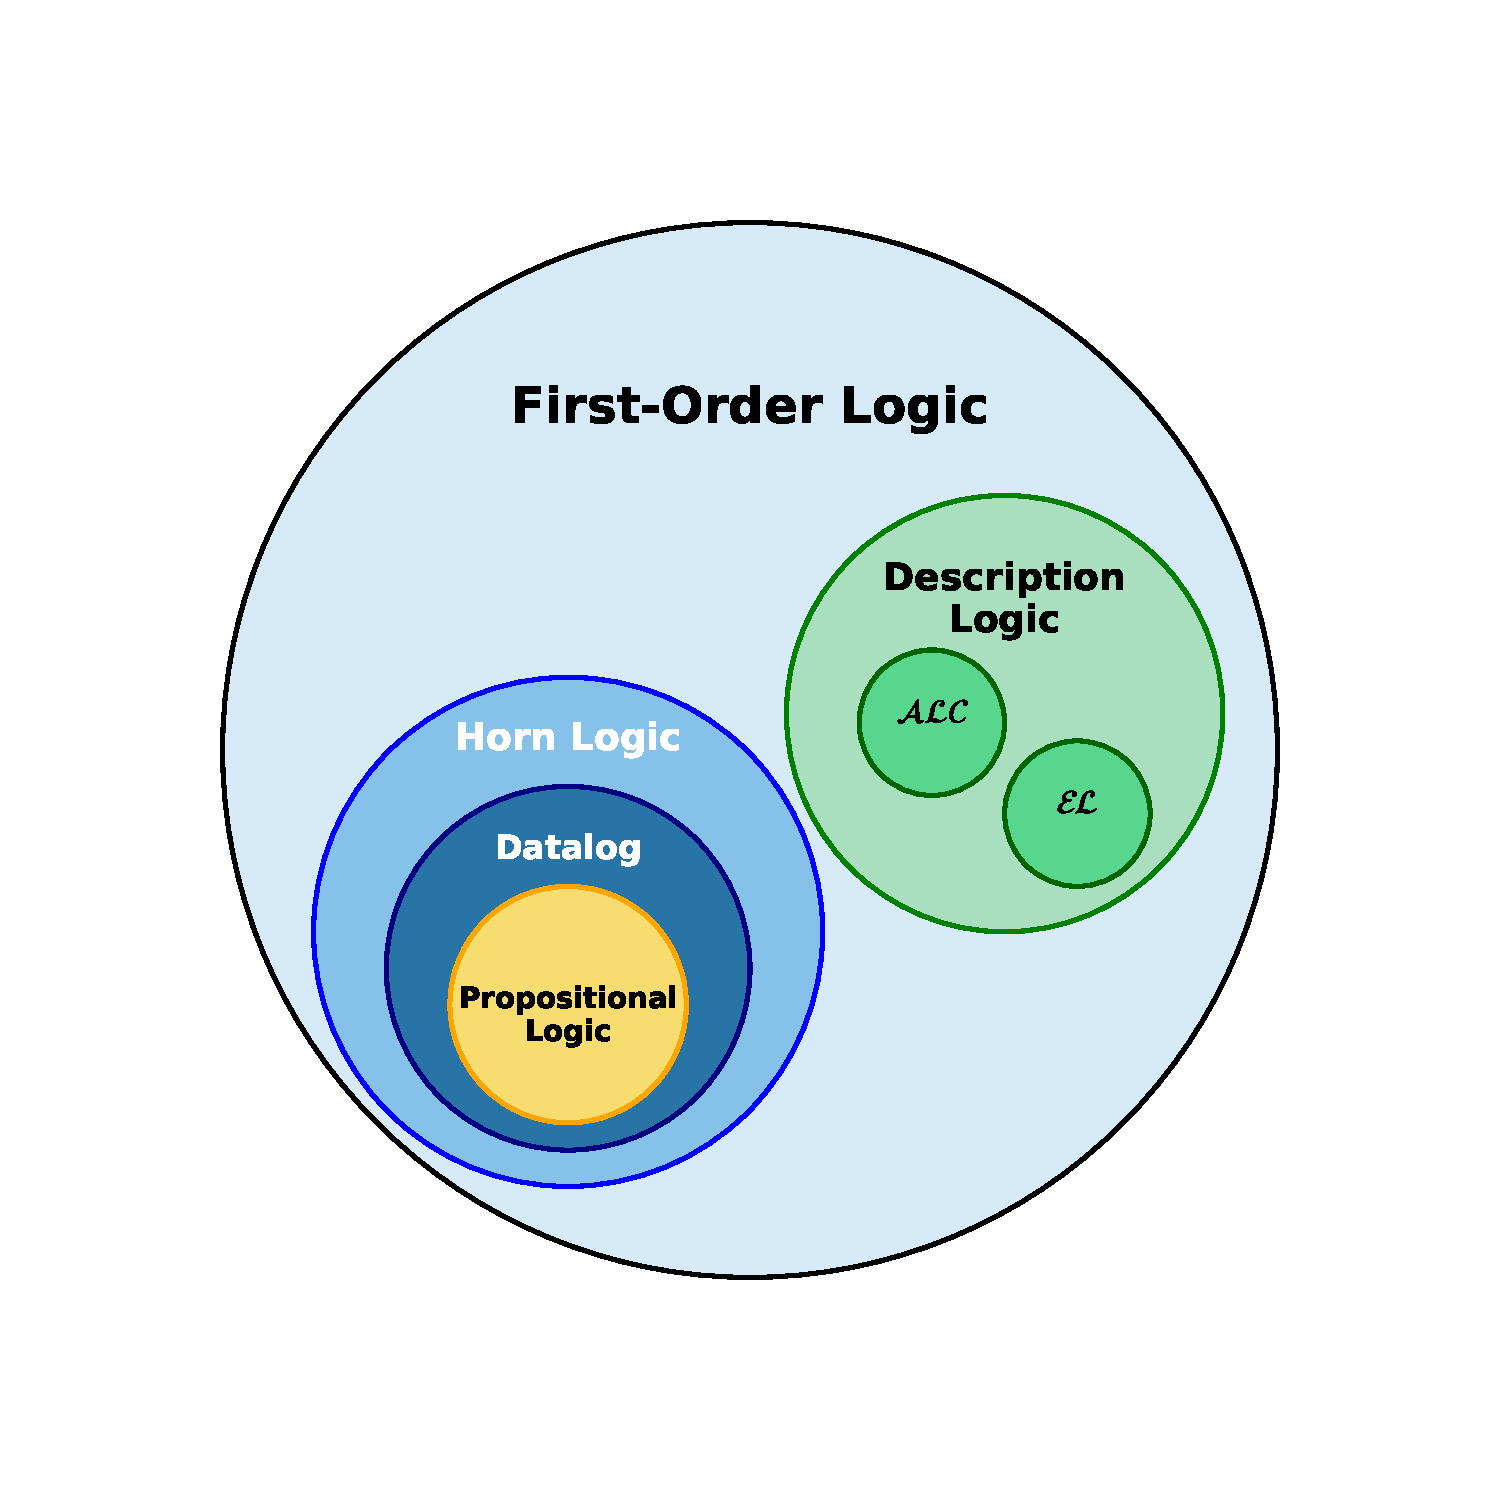
\includegraphics[width=0.58\textwidth]{figures/venn_diagram_logics}
    \caption[Venn diagram of different logic families]{
        %
        Venn diagram of different logic families, illustrating the trade-off between expressiveness and tractability.
        %
        \Gls{FOL} is the most expressive logic -- not the most expressive logic in general -- encompassing all others.
        %
        On the other hand, propositional logic is the least expressive, as it can only represent atomic propositions and their combinations.
        %
        All the other logics fall somewhere in between, with varying degrees of expressiveness and tractability.
    }
    \label{fig:venn-diagram-logics}
\end{SCfigure}

%
Tractability addresses the theoretical question of whether a logic reasoner can determine the truth of a given formula within feasible time and space bounds.
%
The answer is deeply tied to the specific reasoning algorithm and the logic's formal properties.
%
Depending on the features a logic provides -- such as quantifiers, function symbols, or recursive definitions -- it may be more or less expressive.
%
The higher the expressiveness, the more complex the problems that can be represented and reasoned about, but this also increases the computational burden.
%
This well-known phenomenon is often referred to as the expressiveness/tractability trade-off~\cite{DBLP:journals/jlp/CadoliS93,BRACHMAN2004327,DBLP:journals/ci/LevesqueB87}.
%
In practice, highly expressive logics make it easier for human users to model rich domains, often requiring fewer and more concise formulas.
%
However, this comes at the cost of automated inference, which may become computationally intractable, undecidable, or non-terminating in the general case.
%
To mitigate this issue, various fragments and extensions of \gls{FOL} have been identified, each providing different tradeoffs between what can be expressed and what can be decided efficiently.
%
\Cref{fig:venn-diagram-logics} illustrates the relationships among different logic families, highlighting the trade-off between expressiveness and tractability.


\subsection{\Glsentrylong{FOL}}\label{subsec:first-order-logic}
%
\Gls{FOL} is a general-purpose formalism that underpins most symbolic \gls{KR} systems.
%
It enables both human and computational agents to model entities and their interrelations through predicates and terms within a defined domain of discourse.
%
Its syntax comprises variables (quantified explicitly or implicitly), constants, function symbols, and predicate symbols, which are combined via logical operators such as conjunction (\(\wedge\)), disjunction (\(\vee\)), implication (\(\rightarrow\)), and equivalence (\(\leftrightarrow\)).
%
\Gls{FOL} allows for both \emph{extensional} and \emph{intensional} definitions.
%
Recursive intensional definitions, in particular, are powerful, enabling finite representations of infinite sets.
%
Despite its flexibility, \gls{FOL} is semi-decidable in general: there is no algorithm that can determine the truth of every \gls{FOL} formula in finite time, which limits its use in systems requiring guaranteed termination~\cite{DBLP:conf/dlog/2003handbook}.


\subsection{Horn logic}\label{subsec:horn-logic}
%
Horn logic is a significant subset of \gls{FOL}, offering a balanced trade-off between theoretical expressiveness and practical tractability~\cite{DBLP:journals/jcss/Makowsky87}.
%
It is built around the concept of \emph{Horn clauses}~\cite{DBLP:journals/jsyml/Horn51}, which are formulas in \gls{FOL} that exclude quantifiers and consist of a disjunction of predicates, with at most one non-negated literal.
%
Alternatively, a Horn clause can be expressed as an implication where the consequent is a single predicate and the antecedent is a conjunction of predicates: \(h \gets b_1, \dots, b_n\).
%
Here, \(\gets\) denotes logical implication (from right to left), commas represent logical conjunctions, and \(b_i\) as well as \(h\) are predicates of arbitrary arity, potentially containing \gls{FOL} terms such as variables, constants, or functions.

Horn clauses can be interpreted as \emph{if-then} rules written in reverse order, where only conjunctions of predicates are allowed in the antecedent.
%
In essence, Horn logic is a constrained subset of \gls{FOL} characterized by the following limitations:
%
\begin{inlinelist}
%
    \item formulas are reduced to clauses, containing only predicates, conjunctions, and a single implication operator;
    %
    \item operators such as \(\lor\), \(\leftrightarrow\), or \(\neg\) (negation) are not allowed;
    %
    \item variables are implicitly quantified; and
    %
    \item terms behave as they do in \gls{FOL}.
    %
\end{inlinelist}


\subsection{Datalog}\label{subsec:datalog}
%
Datalog is a declarative query language and a restricted subset of \gls{FOL}, designed for deductive databases and knowledge representation~\cite{DBLP:journals/jcss/AjtaiG94}.
%
It represents knowledge using function-free Horn clauses, as defined in \Cref{subsec:horn-logic}.
%
This restriction eliminates the use of function symbols, thereby forbidding structured terms such as recursive data structures.
%
As a result, Datalog is well-suited for applications requiring finite and decidable reasoning, as the absence of function symbols ensures termination of inference algorithms.
%
Similar to Horn logic, Datalog’s knowledge bases consist of sets of function-free Horn clauses, which are interpreted as rules and facts.
%
Rules in Datalog follow the form \(h \gets b_1, \dots, b_n\), where \(h\) is the head of the rule and \(b_1, \dots, b_n\) are the body predicates.
%
Unlike general \gls{FOL}, Datalog does not allow disjunctions, negations, or explicit quantifiers, as variables are implicitly universally quantified.
%
Datalog is widely used in areas such as \glspl{KG}, semantic web technologies, and database systems, where efficient reasoning over large datasets is required.
%
Its simplicity and computational efficiency make it a practical choice for symbolic \gls{AI} tasks that demand tractable reasoning.


\subsection{\Glsentrylong{DL}}\label{subsec:dl}
%
\Gls{DL} are a family of subsets of \gls{FOL}, typically involving limited or no quantifiers, no structured terms, and no \textit{n}-ary predicates where \(n \geq 3\)~\cite{DBLP:books/daglib/0041477}.
%
In essence, \gls{DL} represents knowledge using constants and variables, along with atomic, unary, and binary predicates.


The differences among specific variants of \gls{DL} lie in the set of supported logical connectives and whether negation is allowed.
%
The wide variety of \gls{DL} stems from the well-known trade-off between expressiveness and tractability.
%
Depending on the application, one may prefer a more expressive \gls{DL} variant, which offers richer features at the cost of reduced tractability or even decidability of algorithms manipulating the knowledge, or vice versa.


In \gls{DL}, it is common practice to use specific terminology for different elements of knowledge representation:
%
\begin{itemize}
    %
    \item Constant terms are referred to as \textit{individuals}, as each constant represents a single entity within a domain.
    %
    \item Unary predicates are called \textit{classes} or \textit{concepts}, grouping sets of individuals for which the predicate holds true.
    %
    \item Binary predicates are referred to as \textit{properties} or \textit{roles}, connecting pairs of individuals.
    %
\end{itemize}
%

Using this nomenclature, knowledge in \gls{DL} can be represented by associating entities with constants (e.g., URLs) and defining concepts and properties accordingly.
%
Binary predicates are particularly significant as they enable the connection of pairs of entities.
%
This is typically achieved through subject–predicate–object triplets, represented as ground binary predicates of the form \(\langle a \, f \, b\rangle\) or \(f(a, b)\), where \(a\) is the subject, \(f\) is the predicate, and \(b\) is the object.

Collections of such triplets form \glspl{KG}, which are directed graphs where vertices represent individuals and arcs represent binary properties connecting these individuals.
%
\glspl{KG} may explicitly or implicitly instantiate a specific ontology, which is a formal description of classes characterizing a domain, their relationships (e.g., inclusion, exclusion, intersection, equivalence), and the properties they must or must not include.


\glspl{DL} are widely used in applications such as semantic web~\cite{DBLP:conf/coopis/GangemiM03} and ontology engineering~\cite{DBLP:books/ios/HGJKP2016}, where efficient reasoning and knowledge representation are essential.
%
Their ability to balance expressiveness and computational efficiency makes them a cornerstone of symbolic reasoning systems.


\subsection{Ontologies and \glsentrylong{KG}}\label{subsec:ontologies-and-kg}
%
An ontology is a formal and explicit specification of a shared conceptualisation of a domain~\cite{DBLP:books/daglib/p/Grimm10}.
%
It provides a structured vocabulary to describe the entities relevant in that domain, along with their attributes and the relationships among them.
%
This organisation enables both human understanding and machine-based reasoning.

Ontologies are typically expressed using \glspl{DL}, a family of logic-based formalisms for knowledge representation.
%
\Glspl{DL} define three main components:
%
\begin{inlinelist}
    %
    \item\emph{concepts} (or \emph{classes}), which group entities sharing similar features;
    %
    \item\emph{individuals} (or \emph{instances}), which are the concrete elements of the domain;
    %
    \item\emph{roles} (or \emph{properties}), which describe binary relationships between individuals.
    %
\end{inlinelist}
%
Different \glspl{DL} vary in their expressive power: for example, \gls{EL} supports only conjunction and existential quantification to ensure efficient reasoning, while more expressive DLs like \gls{ALC} allow for full Boolean operators and universal quantification.

Concepts are typically denoted using capital italic letters, such as $\mathit{Animal}$ or $\mathit{Cat}$.
%
These can be combined using logical constructors like intersection ($\sqcap$), union ($\sqcup$), or negation ($\lnot$) to form more complex classes.
%
A statement like $\mathit{Cat} \sqsubseteq \mathit{Animal}$ expresses that all cats are animals.

Individuals are constants representing specific entities in the domain and are usually written in monospaced lowercase, for example \texttt{tom}.
%
Membership of an individual in a concept is denoted using the ``is-a'' relation, written as \texttt{tom}~:~$\mathit{Cat}$, meaning ``Tom is a cat.''
%
Each individual may belong to multiple concepts.

Roles represent binary relations between individuals and are written in lowercase sans-serif font, such as \textsf{eats}.
%
They connect pairs of individuals, and their domain and range can be restricted using expressions such as $\textsf{eats} \sqsubseteq \mathit{Animal} \times \mathit{Edible}$.
%
Assertions like $\textsf{eats}(\texttt{tom}, \texttt{mouse})$ state that Tom eats the mouse.

The subsumption relation ($\sqsubseteq$) is used to express inclusion between concepts or roles.
%
For instance, $\mathit{Cat} \sqsubseteq \mathit{Animal}$ means that every cat is also an animal, and $\textsf{predatorOf} \sqsubseteq \textsf{eats}$ means that every predator-prey relationship implies eating.
%
Special concepts such as $\top$ and $\bot$ are used to denote the most general and the most specific concepts, respectively.

Collections of such axioms form an ontology.
%
\Gls{TBOX} define concepts and roles and their interrelations, while \gls{ABOX} specify which individuals belong to which concepts or are related via which roles.

\Glspl{KG} also provide a structured way to represent knowledge as graphs.
%
They consist of triplets (or \emph{facts}) of the form $(s, p, o)$, where $s$ is the subject, $p$ is the predicate (or property), and $o$ is the object.
%
These triplets form a directed graph where nodes represent individuals and edges represent relationships.

Unlike ontologies, KGs do not necessarily impose formal constraints on the structure or semantics of the triplets.
%
This flexibility allows for representing heterogeneous and incomplete data.
%
However, some \glspl{KG} are explicitly grounded in an ontology, and may follow its vocabulary and logical constraints.

In summary, ontologies and knowledge graphs both aim to formally capture structured knowledge.
%
Ontologies provide formal semantics and enable logical reasoning, while knowledge graphs emphasise scalability and flexibility in representing factual data.


\subsection{Propositional Logic}\label{subsec:propositional-logic}
%
Propositional logic is a restricted subset of \gls{FOL} in which quantifiers, terms, and non-atomic predicates are absent.  
%
Its language consists solely of atomic propositions—also called 0-ary predicates—combined using standard logical connectives such as conjunction ($\land$), disjunction ($\lor$), negation ($\lnot$), and implication ($\rightarrow$).  
%
Each proposition can be interpreted as a Boolean variable that takes a truth value in \{\texttt{true}, \texttt{false}\}.  
%
The semantics of propositional logic aligns with Boolean algebra, making it straightforward to evaluate the truth of a formula given the truth values of its atomic components.

For example, a propositional formula such as $p \land \lnot q \rightarrow r$ can be interpreted as follows:  
%
$p$ might stand for the proposition ``it is raining,'' $q$ for ``there is a roof,'' and $r$ for ``the floor is wet.''  
%
In this case, the formula asserts that if it is raining and there is no roof, then the floor will be wet.

Compared to \gls{FOL}, propositional logic is significantly less expressive.  
%
The absence of quantifiers means that general statements over a domain cannot be made.  
%
Similarly, the lack of terms prevents direct reference to entities in the domain.  
%
As a consequence, each relevant aspect of a scenario must be explicitly encoded as an individual proposition.

This limitation in expressiveness has important computational implications.  
%
In particular, determining the satisfiability of a propositional formula is a decidable problem.  
%
This makes propositional logic attractive in scenarios where tractable reasoning is required.

Despite its apparent simplicity, propositional logic can model a surprising range of situations.  
%
Expressions involving numerical constants, variables, and comparisons (e.g., $x > 5$ or $y = 3$) can be encoded propositionally by introducing a distinct Boolean variable for each comparison.  
%
This reduction allows the use of propositional logic in settings where the original problem does not explicitly involve logical variables or quantifiers, but can be decomposed into atomic truth conditions.


\subsection{Limits of symbolic \Gls{AI}}\label{subsec:limits-of-symbolic-ai}
%



\section{Sub-symbolic \Gls{AI}}\label{sec:sub-symbolic-ai}
%
Sub-symbolic \gls{AI} encompasses a wide range of techniques that rely on numerical representations.
%
Contributions come from varius fields, including \gls{ML}, statistical learning, and data mining.
%
The huge number of approaches is also motivated by the well known \gls{NFL} theorem~\cite{DBLP:journals/tec/DolpertM97} that states that no single learning algorithm can outperform all others across all possible tasks.
%
The most common predictor families are linear models, \glspl{DT}, \glspl{RF}, \glspl{SVM}, \glspl{NN} (including \glspl{LLM}), and many others.


\paragraph{Predictive performance vs. interpretability}
%
\begin{figure}[h]
    \centering
    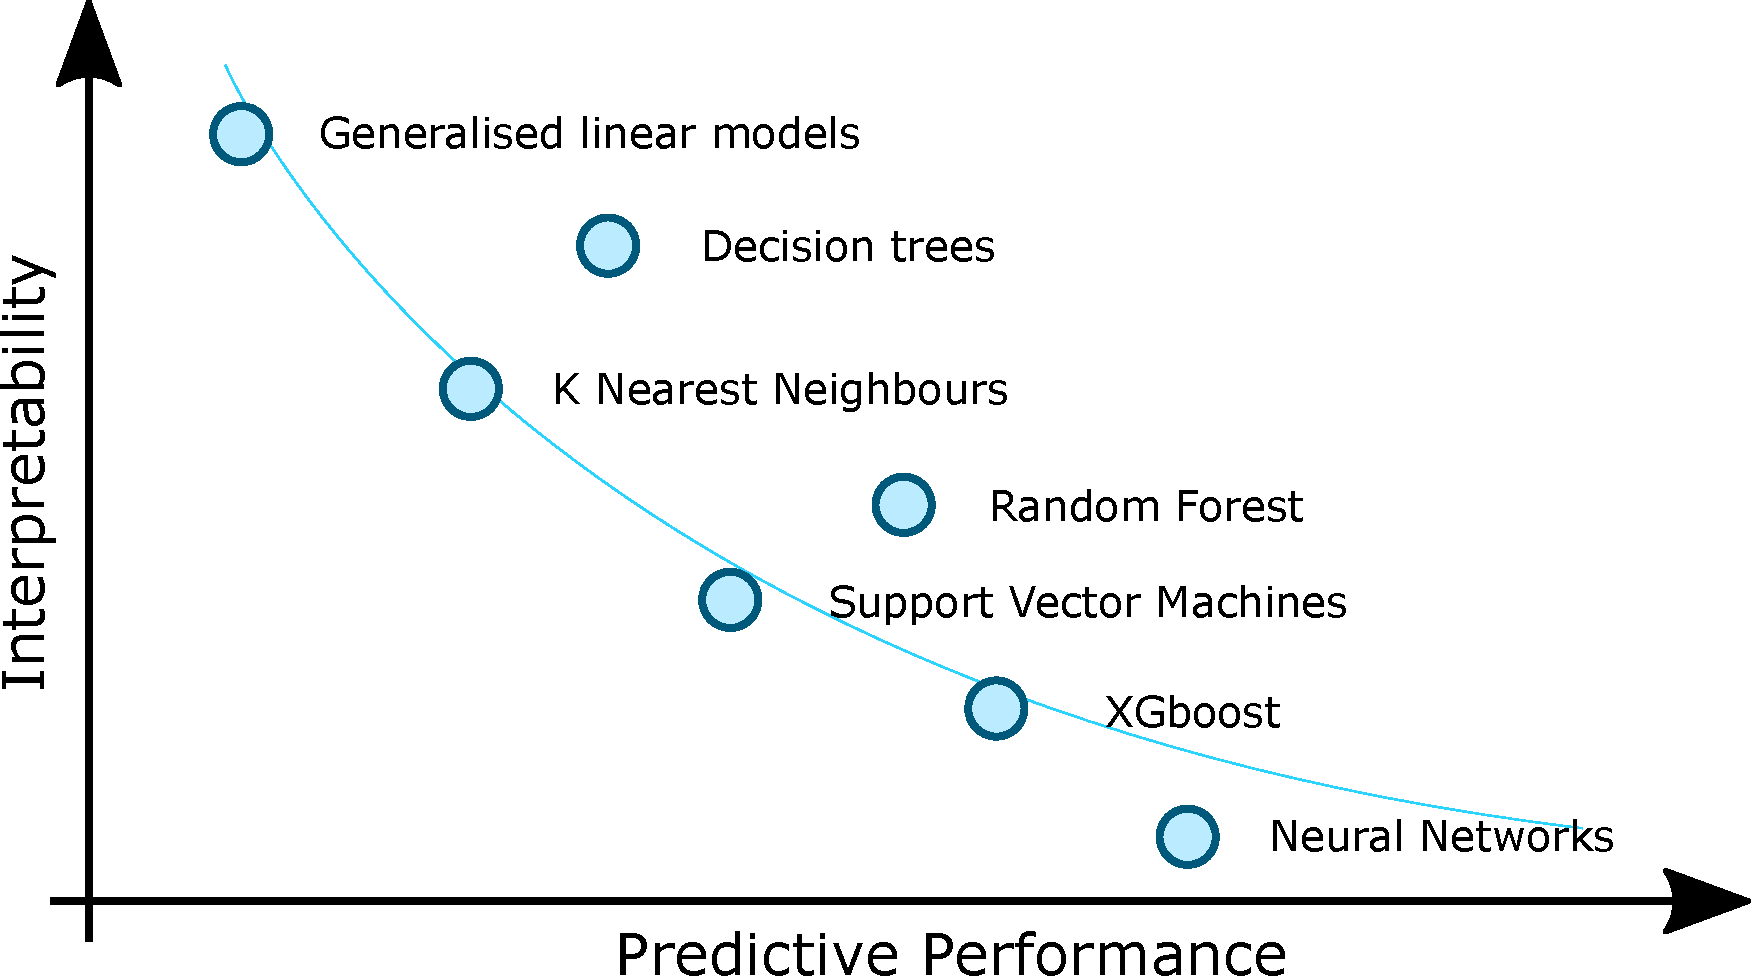
\includegraphics[width=0.9\textwidth]{figures/interpretability-performance-tradeoff}
    \caption[Performance vs. interpretability trade-off]{
        %
        Trade-off between predictive performance and interpretability in common sub-symbolic predictors.
        %
        The figure illustrates how different predictor families balance these two aspects, with simpler models being more interpretable but potentially less accurate.
        %
    }
    \label{fig:performance-vs-interpretability}
\end{figure}
%
The \emph{complexity} of a sub-symbolic predictor can vary significantly.
%
By complexity we mean the overall structure of the model, including the number of parameters, the operations that are performed, and possibly the way the model is trained.
%
\Glspl{DT}, for example, are relatively simple models that can be easily interpreted by humans.
%
The downside of \glspl{DT} is that they make predictions by linearly partitioning the input space, which can lead to poor generalisation on unseen data.
%
On the other hand, \glspl{NN} can be extremely complex, with millions of parameters and intricate architectures that are difficult to interpret.
%
However, \glspl{NN} can capture highly non-linear relationships in the data, often leading to superior predictive performance compared to simpler models.
%
The definition of interpretability is not univocal, and it lacks measures that are widely accepted~\cite{DBLP:journals/natmi/Rudin19}.
%
Despite that, \Cref{fig:performance-vs-interpretability} illustrates in an informal way the trade-off between predictive performance and interpretability in sub-symbolic predictors.


\subsection{\Glsentrylongpl{DT}}\label{subsec:decision-trees}

\subsection{\Glsentrylongpl{RF}}\label{subsec:random-forests}

\subsection{\Glsentrylongpl{SVM}}\label{subsec:svm}

\subsection{\Glsentrylongpl{NN}}\label{subsec:neural-networks}

\subsection{Limits of sub-symbolic \Gls{AI}}\label{subsec:limits-of-sub-symbolic-ai}
%! Author = matteomagnini
%! Date = 05/03/25

%----------------------------------------------------------------------------------------
\chapter{Neuro-symbolic AI}
\label{ch:nesy-ai}
\minitoc
%----------------------------------------------------------------------------------------

\section[Symbolic knowledge injection]{\Glsentrylong{SKI}}\label{sec:ski}
%
\Gls{SKI} is a wide sub-field of \gls{NeSy}, which encompasses all the methods that in some way \emph{inject} symbolic knowledge into sub-symbolic predictors.
%
More precisely, we define \gls{SKI} as:
%
\begin{definition}[\gls{SKI}]
    \label{def:ski}
    any algorithmic procedure affecting how sub-symbolic predictors draw their inferences in such a way that predictions are either \textbf{computed} as a function of, or \textbf{made consistent} with, some given symbolic knowledge~\cite{DBLP:journals/csur/CiattoSAMO24}.
\end{definition}
%
We adopt this broad definition because the amount of works in the literature is vast and varied, furthermore the contributions come from different communities (e.g., \gls{ML}, \gls{AI}, \gls{NLP}, \gls{XAI}, logics, etc.), and they often use different terminologies.


\subsection{Motivations and goals}\label{subsec:ski-motivations-and-goals}
%
\Gls{SKI} can be used for several reasons, such as:
%
\begin{inlinelist}
    %
    \item \label{itm:prediction}\emph{improving the model's predictive performance}, by leveraging symbolic knowledge to guide their learning or inference;
    %
    \item \label{itm:interpretability}\emph{improving the model's interpretability}, by making their predictions consistent with symbolic knowledge;
    %
    \item \label{itm:robustness}\emph{increase the robustness} of sub-symbolic predictors, by making them less sensitive to data perturbations (e.g., noise, data scarcity, etc.);
    %
    \item \label{itm:complexity}\emph{reduce the model complexity} of the models, by shaping their structure or by constraining their parameters;
    %
    \item and possibly many more.
    %
\end{inlinelist}


\Cref{itm:prediction} is one of the most common motivations for \gls{SKI}.
%
The idea is simple: if there is already some (symbolic) knowledge about a particular domain or task, then it is reasonable to expect that the predictor can benefit from it.
%
In this way the model learns both from the data -- inductively -- and from the symbolic knowledge---mimicking deductive reasoning.


Another common reason to use \gls{SKI} is to increase the \emph{interpretability} of the model, as stated in \Cref{itm:interpretability}.
%
In the context of \gls{XAI}, this is usually referred as \gls{XAI} \emph{by design} (\Cref{par:xai-by-design}).
%
The intuition is simple: the model is made to be consistent -- up to a certain extent -- with the symbolic knowledge, which is usually more interpretable than the model itself.
%
This can be done in two ways: either by using \emph{symbols as constraints} or by \emph{transparent box design}.
%
More details about these two approaches are provided in \Cref{subsec:learning} and \Cref{subsec:structuring}, respectively.


Predictive performances and \gls{XAI} are the main motivations for \gls{SKI}, but not the only ones.
%
The \emph{robustness} (\Cref{itm:robustness}) of a predictive model is another important challenge~\cite{DBLP:conf/eccv/LiuCZH18}, and it relates to predictors' ability to maintain performance despite the presence of input perturbations.
%
A metric of robustness in the context of \gls{SKI} is defined in the work ``An Empirical Study on the Robustness of Knowledge Injection Techniques Against Data Degradation''~\cite{DBLP:conf/woa/RafanelliMACO24}.
%
The content of the paper is presented in~\Cref{subsec:empirical-study-on-the-robustness-of-ski-methods}.
%
Along with robustness, there are other metrics -- often neglected -- that play a crucial role in the design of intelligent systems, such as \emph{memory footprint} (\Cref{itm:complexity}), \emph{latency}, data efficiency, and so on.
%
These \gls{QoS} metrics are presented in the work ``Symbolic Knowledge Injection Meets Intelligent Agents: QoS metrics and experiments''~\cite{DBLP:journals/aamas/AgiolloRMCO23}, which is discussed in~\Cref{subsec:ski-meets-intelligent-agents}.


\subsection{What to inject}\label{subsec:what-to-inject}
%
\begin{SCfigure}
    \centering
    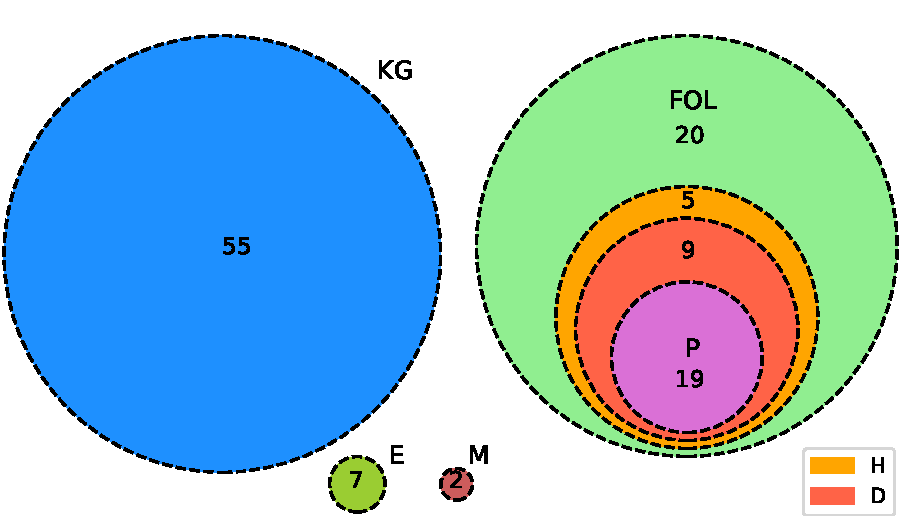
\includegraphics[width=.4\linewidth]{figures/ski-logic}
    \caption[Venn diagram categorising SKI methods]{
        Venn diagram categorising SKI methods w.r.t.\ the \emph{input knowledge} type: knowledge graphs (KG), propositional logic (P), first-order logic (FOL), expert knowledge (E), Datalog (D), Horn logic (H), or modal logic (M).
        %
        The image is taken from~\cite{DBLP:journals/csur/CiattoSAMO24} and it refers to 117 surveyed \gls{SKI} methods.
    }
    \label{fig:pie-ski-logic}
\end{SCfigure}

%
A key distinction in \gls{SKI} methods lies in whether the chosen formalism is \emph{machine interpretable}, \emph{human interpretable}, or both.
%
\Gls{SKI} methods can be categorized into two primary groups based on the formalism used to represent input knowledge~\cite{DBLP:journals/csur/CiattoSAMO24}:
%
\begin{itemize}
    \item \textbf{Logic formulas or \glspl{KB}:} These adhere to \gls{FOL} or its subsets, making them interpretable by both humans and machines.
    %
    The sub-categories, ordered by decreasing expressiveness, include:
    %
    \begin{itemize}
        %
        \item \emph{\gls{FOL} formulas:} These encompass recursive terms, variables, predicates of any arity, and various logic connectives, potentially expressing definitions.
        %
        \item \emph{Horn logic:} Often referred to as Prolog-like logic, this formalism consists of head–body rules involving predicates and terms of any kind.
        %
        \item \emph{Datalog:} A restricted subset of Horn logic that excludes recursive terms, allowing only constants or variables as terms.
        %
        \item \emph{Modal logics:} These extend the above logics with modal operators (e.g., \(\square\) and \(\lozenge\)), which express modalities such as necessity or possibility.
        %
        \item \emph{Knowledge graphs:} A practical application of description logics designed to represent entity–relation graphs.
        %
        \item \emph{Propositional logic:} This involves Boolean variables and logical connectives, offering a simpler yet effective formalism.
    \end{itemize}
    %
    \item \textbf{Expert knowledge:} This category includes human-interpretable knowledge that is not inherently machine-readable.
    %
    Examples include physics equations, syntactical rules, or domain-specific expertise.
    %
    Since expert knowledge is not directly machine interpretable, it often requires transformation into tensorial form through data generation, a process that typically involves human engineers and can be labor-intensive.
\end{itemize}
%
\Cref{fig:pie-ski-logic} illustrates the distribution of surveyed \gls{SKI} methods based on their formalism of choice.
%
\Glspl{KG} emerge as the most prevalent category, representing nearly half of the surveyed methods.
%
In contrast, modal logics constitute the smallest group.
%
Methods based on \gls{FOL} or its subsets (excluding \glspl{KG}) form another significant cluster, with propositional logic being particularly prominent due to its relative simplicity and widespread use.
%
The specific logic formalism employed in the surveyed papers is reported where available.
%
However, this information is rarely explicitly stated by the authors.
%
Instead, the logic is often inferred from the constraints and descriptions provided in the respective works.

Practical examples of symbolic knowledge that can be injected into sub-symbolic predictors are the public health guidelines on type-2 diabetes of the National Institute of Diabetes and Digestive and Kidney Diseases\footnote{\url{https://www.niddk.nih.gov/health-information/diabetes/}}.
%
These guidelines have been encoded into logic formulas~\cite{DBLP:conf/pkdd/KunapuliBSMS10} and used in works related to \gls{SKI}~\cite{Magnini-telmed2025}.
%
The first guideline state that if a patient has a glucose value greater or equal to 125 mg/dL and a \gls{BMI} greater or equal to 30, then the patient is considered diabetic.
%
The second one says that if a patient has a glucose value lower or equal to 100 mg/dL and a \gls{BMI} lower or equal to 25, then the patient is considered non-diabetic.
%
In \gls{FOL}, the first statement can be encoded as:
%
\begin{equation}\label{eq:rule-diabetic}
  \forall x . ( \text{glucose}(x) \geq 125 \land \text{bmi}(x) \geq 30 \rightarrow \text{Diabetic}(x))
\end{equation}
%
whereas the second statement can be encoded as:
%
\begin{equation}\label{eq:rule-not-diabetic}
  \forall x . ( \text{glucose}(x) \leq 100 \land \text{bmi}(x) \leq 25 \rightarrow \neg \text{Diabetic}(x))
\end{equation}


\subsection{How to inject}\label{subsec:how-to-inject}
%



\subsection{Structuring}\label{subsec:structuring}

\subsection{Learning}\label{subsec:learning}

\subsection{Embedding}\label{subsec:ski-embedding}

\subsection[Limitations and challenges of SKI]{Limitations and challenges of \Gls{SKI}}\label{subsec:limitations-and-challenges-of-ski}

\section[Symbolic knowledge extraction]{\Glsentrylong{SKE}}\label{sec:ske}

\subsection{Motivations and goals}\label{subsec:ske-motivations-and-goals}

\subsection{How to extract}\label{subsec:how-to-extract}

\subsection[Decompositional SKE]{Decompositional \Gls{SKE}}\label{subsec:decompositional-ske}

\subsection[Pedagocial SKE]{Pedagocial \Gls{SKE}}\label{subsec:pedagogical-ske}

\subsection{Local explanations}\label{subsec:local-explanations}

\subsection{Global explanations}\label{subsec:global-explanations}

\subsection[Limitations and challenges of SKE]{Limitations and challenges of \Gls{SKE}}\label{subsec:limitations-and-challenges-of-ske}
%! Author = matteomagnini
%! Date = 05/03/25

%----------------------------------------------------------------------------------------
\chapter{Large Language Models}
\label{ch:llm}
\minitoc
%----------------------------------------------------------------------------------------

\section{Architectures}\label{sec:llm-architectures}

\subsection{Transformer}\label{subsec:transformer}

\subsection{Attention}\label{subsec:attention}

\section{Fine-tuning}\label{sec:llm-fine-tuning}

\section{\Glsentrylong{RAG}}\label{sec:rag}

\subsection{Embedding}\label{subsec:rag-embedding}

\subsection{Retrieval}\label{subsec:retrieval}

\section{Limitations and challenges}\label{sec:limitations-and-challenges}

\subsection{Resources}\label{subsec:resources}

\subsection{Data and privacy}\label{subsec:data-and-privacy}

\subsection{Hallucinations}\label{subsec:hallucinations}

\subsection{Stochastic parrot or something more?}\label{subsec:stochastic-parrot-or-something-more}
\printbibliography[title=References,heading=bibintoc]
\end{refsection}

%----------------------------------------------------------------------------------------
%-------------------------------------- PART II -----------------------------------------
%----------------------------------------------------------------------------------------

\part{Methods and Platform for \gls{SKI} \& \gls{SKE}}
\label{part:engineering-of-ski-ske}

\begin{refsection}
%! Author = matteomagnini
%! Date = 05/03/25

%----------------------------------------------------------------------------------------
\chapter{SKI: methods and contributions}
\label{ch:ski-methods-and-contributions}
\minitoc
%----------------------------------------------------------------------------------------

In this chapter we present two main algorithmic contributions to the field of \gls{SKI}.
%
First, we provide the motivations behind the design and development of these contributions in \Cref{sec:ski-motivations}.
%
Second, we detail the contributions themselves in \Cref{sec:ski-contribution-kill,sec:ski-contribution-kins}, and we report the results of the empirical evaluation of these contributions.
%
Finally, we discuss the implications of these contributions and outline future directions in \Cref{sec:ski-discussion-and-future-direction}.


\section{Motivations}\label{sec:ski-motivations}
%
Aware by the limitations reported in \Cref{subsec:limitations-and-challenges-of-ski}, we wanted to develop novel \gls{SKI} methods that could be used in many different domains.
%
For this reason, these methods include all the elements described in \Cref{subsec:how-to-inject}.
%
In particular, a \emph{parser} is provided to convert symbolic knowledge into a format that can be injected into a neural network.
%
In this way, we are not bounded to a specific knowledge base nor to a specific domain.
%
The transformation of the parsed rules into a numeric interpretation is automatically performed by a \emph{fuzzification step}.
%
Finally, the sub-symbolic component is injected into a neural network, which is trained to learn the symbolic knowledge.
%
Another limitation that we wanted to address is the expressiveness of the symbolic knowledge that can be injected.
%
What we target in these two works is knowledge expressed in \emph{stratified Datalog with negation}.


\subsection{Stratified Datalog with negation}\label{subsec:skistratified-datalog-with-negation}
%
This logic is a variant of Datalog~\cite{DBLP:books/mc/18/MaierTKW18} with no recursion -- neither direct nor indirect -- yet supporting negated atoms.
%
We choose Datalog because of its expressiveness (strictly higher than propositional logic) and its acceptable limitations.
%
The lack of recursion, in particular, prevents issues when it comes to convert formulas into neural structures (which are \glspl{DAG}).
%
Since we rely on Datalog with negation, we allow atoms in the bodies od clauses to be negated.
%
Using the same notation as in \Cref{subsec:datalog}, in case the $i^{th}$ atom in the body of some clause is negated, we write $\neg b_{i}$.
%
There, each atom $h$, $b_{1}$, $b_{2}$, \dots{} may be a predicate of arbitrary arity.

An \(l\)-ary predicate \(p\) denotes a relation among \(l\) entities: \(p(t_1, \dots, t_l)\), where each \(t_i\) is a term, i.e., either a constant (denoted in \texttt{monospace}) representing a particular entity, or a logic variable (denoted by \textit{Capitalised Italic}) representing some unknown entity or value.
%
Well-known binary predicates – e.g., \(>\), \(<\), \(=\) – are admissible, too, and retain their usual semantics from arithmetic.
%
For the sake of readability, we may write these predicates in infix form—hence \(>(X, 1) \equiv X > 1\).

To support injection into a particular \gls{NN}, we further assume the input knowledge base defines one (and only one) outer relation -- say \texttt{output} or \texttt{class} -- involving as many variables as the input and output features the \gls{NN} has been trained upon.
%
That relation must be defined via one clause per output neuron.
%
Yet, each clause may contain other predicates in their bodies, in turn defined by one or more clauses.
%
In that case, since we rely on stratified Datalog, we require the input knowledge to not include any (directly or indirectly) recursive clause definition.

For example, for a 3-class classification task, any provided knowledge base should include a clause such as the following one:
%
\begin{align*}
    \texttt{class}(\bar{X}, y_1) &\leftarrow \texttt{p}_1(\bar{X}) \land \texttt{p}_2(\bar{X}) \\
    \texttt{p}_1(\bar{X}) &\leftarrow \dots \\
    \texttt{p}_2(\bar{X}) &\leftarrow \dots \\
    \texttt{class}(\bar{X}, y_2) &\leftarrow \texttt{p}'_1(\bar{X}) \land \texttt{p}'_2(\bar{X}) \\
    \texttt{p}'_1(\bar{X}) &\leftarrow \dots \\
    \texttt{p}'_2(\bar{X}) &\leftarrow \dots \\
    \texttt{class}(\bar{X}, y_3) &\leftarrow \texttt{p}''_1(\bar{X}) \land \texttt{p}''_2(\bar{X}) \\
    \texttt{p}''_1(\bar{X}) &\leftarrow \dots \\
    \texttt{p}''_2(\bar{X}) &\leftarrow \dots
\end{align*}
%
where \(\bar{X}\) is a tuple having as many variables as the neurons in the output layer, \(y_i\) is a constant denoting the \(i\)-th class, and \(\texttt{p}_1\), \(\texttt{p}_2\), \(\texttt{p}'_1\), \(\texttt{p}'_2\), \(\texttt{p}''_1\), \(\texttt{p}''_2\) are ancillary predicates defined via Horn clauses as well.


\section{Knowledge injection via lambda layer}\label{sec:ski-contribution-kill}
%
In this section we present the paper ``A view to a KILL: Knowledge Injection via Lambda Layer''~\cite{DBLP:conf/woa/MagniniCO22}, presented at the 23rd Workshop ``From Objects to Agents'' (WOA 2022)~\footnote{\url{https://sites.google.com/view/woa2022/}}.
%
The paper introduces a novel \gls{SKI} method, called \gls{KILL}, which allow to inject symbolic knowledge in stratified Datalog with negation into \glspl{NN} of any shape.
%
\Gls{KILL} does not require the input formulas to be \emph{ground}, and it does not impose any constraint on the \gls{NN} undergoing injection.
%
The method acts directly at the backpropagation level, by increasing the penalty to be back-propagated whenever the \gls{NN} output is violating the knowledge to be injected.
%
For this reason, \gls{KILL} falls under the \emph{guided learning} strategy, as described in \Cref{subsec:how-to-inject}.


\subsection{$\Lambda$-layer}\label{subsec:lambda-layer}
%
\begin{figure}
    \centering
    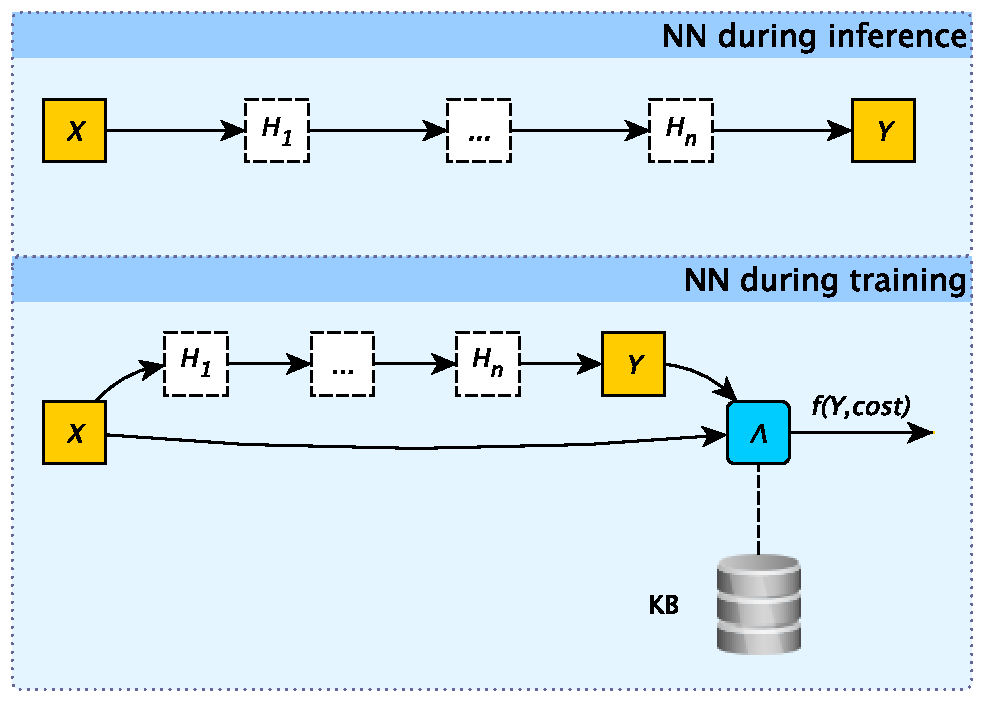
\includegraphics[width=0.8\linewidth]{figures/lambda-layer}
    \caption[General architecture of a NN with $\Lambda$-layer]{
        General architecture of a \gls{NN} with $n$ hidden layers, $X$ and $Y$ are respectively the input and output layers.
        %
        Before training, \gls{KILL} is applied to the predictor so that a new model constrained by the knowledge base (KB) is obtained.
        %
        The $\Lambda$-layer is added to the output layer, and then removed for the inference phase.
    }
    \label{fig:lambda-layer}
\end{figure}
%
The idea behind \gls{KILL} is to perform injection during training.
%
The injection is performed by appending one further layer -- the \emph{$\Lambda$-layer} -- at the output end of the \gls{NN}, and by training the overall network as usual (e.g., via gradient descent or similar).
%
The $\Lambda$-layer introduces an error whenever the prediction from the network's output layer violates the symbolic knowledge being injected.
%
This error influences the gradient descent or other optimization functions, discouraging violations of the symbolic knowledge.
%
In essence, the \gls{NN} learns inductively to avoid wrong predictions by penalizing violations during training.
%
To achieve this, the $\Lambda$-layer employs a custom activation function that modifies the output of the network's original output layer.
%
Additionally, the symbolic knowledge must be numerically interpreted, converting logical formulas into real-valued functions to compute error values.
%
Once the training phase is complete, the $\Lambda$-layer can be removed, leaving the original network architecture intact.


To elaborate on the $\Lambda$-layer, we consider a symbolic knowledge base, denoted as \(\mathcal{K}\), to be injected into a feedforward \gls{NN} of arbitrary depth, denoted as \(\mathcal{N}\).
%
Let \(\mathcal{N}\) have an input layer \(\mathbf{X}\) and an output layer \(\mathbf{Y}\), where \(\mathbf{Y}\) is assumed to be of shape \(n \times 1\).
%
This discussion applies to layers of any shape, including multidimensional ones.
%
No assumptions are made about the activation function of \(\mathbf{Y}\), the topology or nature of the hidden layers, or the shape of \(\mathbf{X}\).
%
The output of \(\mathbf{Y}\) is denoted as \(\mathbf{y} = [y_1, \dots, y_n]\), representing the network's prediction for a given input \(\mathbf{x}\).
%
The knowledge base \(\mathcal{K}\) consists of \(n\) rules, \(\mathcal{K} = \{\varphi_1, \dots, \varphi_n\}\), where each rule \(\varphi_i\) constrains the relationship between \(\mathbf{x}\) and \(y_i\).


To inject \(\mathcal{K}\), the $\Lambda$-layer is added to the network architecture, as illustrated in \Cref{fig:lambda-layer}.
%
This layer is densely connected to both \(\mathbf{X}\) and \(\mathbf{Y}\), and its activation function introduces a penalty on \(y_i\) whenever the corresponding rule \(\varphi_i\) is violated for an input-output pair \((\mathbf{x}, \mathbf{y})\).
%
The output of the $\Lambda$-layer, denoted as \(\boldsymbol{\lambda}\), is defined as:
%
\[
\boldsymbol{\lambda} = \mathbf{y} \times (1 + \mathbf{C}(\mathbf{x}, \mathbf{y}))
\]
%
where \(\mathbf{C}(\mathbf{x}, \mathbf{y})\) is a positive penalty vector representing the cost of modifying the network's output \(\mathbf{y}\).
%
The penalty vector \(\mathbf{C}(\mathbf{x}, \mathbf{y})\) is given by:
%
\[
\mathbf{C}(\mathbf{x}, \mathbf{y}) = [c_1(\mathbf{x}, y_1), \dots, c_i(\mathbf{x}, y_i), \dots, c_n(\mathbf{x}, y_n)]
\]
%
where \(c_i : \mathbf{X} \times \mathbf{Y} \to [0, 1]\) interprets the rule \(\varphi_i\) as a cost in the range \([0, 1]\) for the given values of \(\mathbf{x}\) and \(y_i\).
%
A penalty is applied to the \(i\)-th neuron of \(\mathbf{Y}\) whenever the corresponding rule \(\varphi_i\) is violated.
%
The penalty is higher when the violation is severe and approaches zero when the violation is minimal or absent.


\subsection{KILL fuzzifier}\label{subsec:kill-fuzzifier}
%
% !TeX spellcheck = en_GB
% !TeX root = ../phd-thesis.tex

\begin{table}
    \centering
    %
    \begin{tabular}{l|r||cl|r}
        \textbf{Formula} & \textbf{C. interpretation} & & \textbf{Formula} & \textbf{C. interpretation}
        \\
        \hline\hline
        $\llbracket\neg \phi\rrbracket$ & $\eta(1 - \llbracket\phi\rrbracket)$ & & $\llbracket\phi \le \psi\rrbracket$  & $\eta(\llbracket\phi\rrbracket - \llbracket\psi\rrbracket)$
        \\
        $\llbracket\phi  \wedge \psi\rrbracket$ &  $\eta(max(\llbracket\phi\rrbracket, \llbracket\psi\rrbracket))$ & & $\llbracket \pred{class}(\bar{X}, \const{y}_i) \leftarrow \psi \rrbracket$ & $\llbracket \psi \rrbracket^{*}$
        \\
        $\llbracket\phi  \vee \psi\rrbracket$ & $\eta(min(\llbracket\phi\rrbracket, \llbracket\psi\rrbracket))$ & & $\llbracket \text{expr}(\bar{X}) \rrbracket$ & $\text{expr}(\llbracket\bar{X}\rrbracket)$
        \\
        $\llbracket\phi = \psi\rrbracket$ & $\eta(|\llbracket\phi\rrbracket-\llbracket\psi\rrbracket|)$ & & $\llbracket \mathtt{true} \rrbracket$ & $0$
        \\
        $\llbracket\phi \ne \psi\rrbracket$ & $\llbracket \neg ( \phi = \psi )\rrbracket$ & & $\llbracket \mathtt{false} \rrbracket$ & $1$
        \\
        $\llbracket\phi > \psi\rrbracket$  & $\eta(0.5 - \llbracket\phi\rrbracket + \llbracket\psi\rrbracket) $ & & $\llbracket X \rrbracket$ & $x$
        \\
        $\llbracket\phi \ge \psi\rrbracket$ & $\eta(\llbracket\psi\rrbracket - \llbracket\phi\rrbracket)$ & & $\llbracket \const{k} \rrbracket$ & $k$
        \\
        $\llbracket\phi < \psi\rrbracket$  &  $\eta(0.5 + \llbracket\phi\rrbracket - \llbracket\psi\rrbracket)$ & & $\llbracket \pred{p}(\bar{X}) \rrbracket^{**}$ & $\llbracket \psi_1 \vee \ldots \vee \psi_k \rrbracket$
        
    \end{tabular}
    %
    \begin{center}\scriptsize
        $^{*}$ encodes the penalty for the $i^{th}$ neuron
        \\
        \smallskip
        $^{**}$ assuming predicate $p$ is defined by $k$ clauses of the form:
        \\
        $\pred{p}(\bar{X}) \leftarrow \psi_1,\ \ldots,\ \pred{p}(\bar{X}) \leftarrow \psi_k$
    \end{center}
    %
    \caption[KILL Fuzzifier: Logic Formulae Encoding]{
        Logic formulas' encoding into real-valued functions.
        %
        There, $X$ is a logic variable, while $x$ is the corresponding real-valued variable, whereas is $\bar{X}$ a tuple of logic variables.
        %
        Similarly, $\const{k}$ is a numeric constant, and $k$ is the corresponding real value, whereas $\const{k}_i$ is the constant denoting the $i^{th}$ class of a classification problem.
        %
        Finally, $\text{expr}(\bar{X})$ is an arithmetic expression involving the variables in $\bar{X}$.
    }
    %
    \label{tab:kill-logic-formulae}
    %
\end{table}
%
\begin{figure*}[t]
    \centering
    \def\astscale{0.4}
    \begin{minipage}[c]{0.4\textwidth}
        \centering
        \begin{subfigure}{\linewidth}
            \centering
            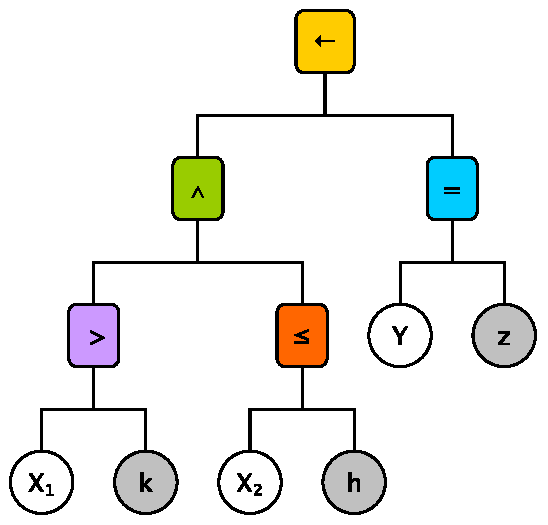
\includegraphics[scale=\astscale]{figures/ast-unencoded}
            \subcaption{AST of a logic formula}
            \label{fig:ast-unencoded}
        \end{subfigure}
        \vspace{1.5ex}
        \tikz{\draw[->, thick] (0,0) -- (0,-0.4);}
        \vspace{2ex}
        \begin{subfigure}{\linewidth}
            \centering
            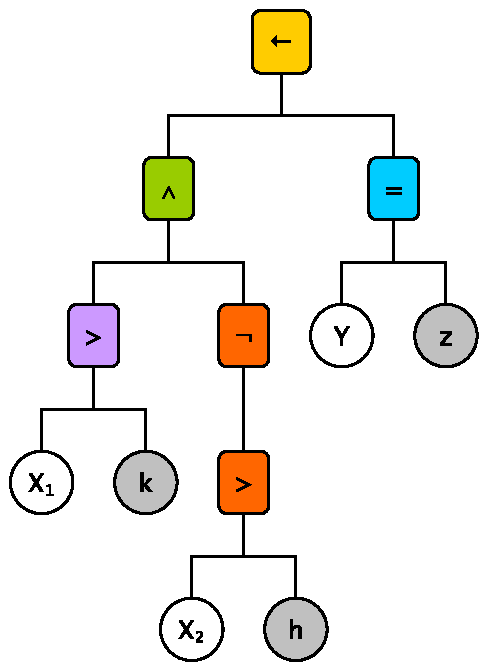
\includegraphics[scale=\astscale]{figures/ast-simplified}
            \subcaption{Simplified AST of a logic formula}
            \label{fig:ast-simplified}
        \end{subfigure}
    \end{minipage}
    \hspace{0.5cm}
    \raisebox{-1cm}{\tikz{\draw[->, thick] (0,0) -- (0.7,0);}}
    \hspace{0.5cm}
    \begin{minipage}[c]{0.4\textwidth}
        \centering
        \begin{subfigure}{\linewidth}
            \centering
            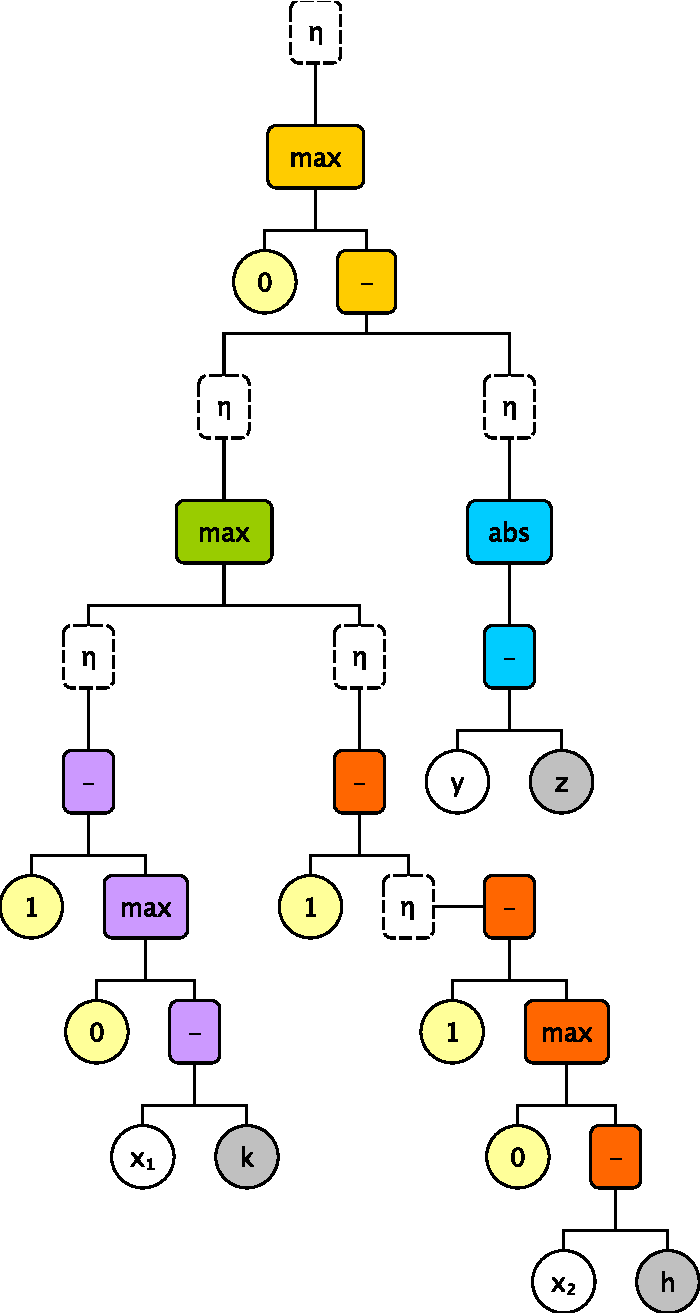
\includegraphics[scale=\astscale]{figures/ast-encoded}
            \subcaption{AST of the same formula, encoded as real-valued function}
            \label{fig:ast-encoded}
        \end{subfigure}
    \end{minipage}
    \caption{
        Example of the encoding process of logic formulas into real-valued functions.
        %
        Only \gls{AST} are depicted.
        %
        Boxes coloured in the same way represent the encoding of a given operator through each encoding step.
        %
        For instance, operator $<$ (red) is first converted into a negated $\geq$, and then into a combination of $max$ and subtractions.
    }
    \label{fig:ast}
\end{figure*}

%
Before injecting symbolic knowledge into a neural network, each formula associated with an output neuron must be converted into a real-valued function to compute the cost of violating that formula.

This conversion relies on a multivalued interpretation of logic inspired by \L{}ukasiewicz's logic~\cite{DBLP:journals/jsyml/Hay63}.
%
Each formula is encoded using the \(\llbracket \cdot \rrbracket\) function, which maps logical formulas to real-valued functions.
%
These functions accept real vectors of size \(m + n\) as input and return scalars in \(\mathbb{R}\) as output.
%
The resulting scalars are clipped to the \([0, 1]\) range using the \(\eta : \mathbb{R} \to [0, 1]\) function, defined as:
%
\begin{align*}
    \eta(x) =
    \begin{cases}
        0 & \text{if } x \leq 0, \\
        x & \text{if } 0 < x < 1, \\
        1 & \text{if } x \geq 1.
    \end{cases}
\end{align*}

The values obtained from \(\eta(x)\) represent penalties, as discussed in \Cref{subsec:lambda-layer}.
%
The penalty for the \(i^{\text{th}}\) neuron violating rule \(\varphi_i\) is expressed as \(c_i(\mathbf{x}, y_i) = \eta(\llbracket \varphi_i \rrbracket(\mathbf{x}, y_i))\).

The \(\llbracket \cdot \rrbracket\) encoding function is recursively defined in \Cref{tab:logic-formulae}.
%
To compute the penalty \(c_i(\mathbf{x}, y_i)\) for the \(i^{\text{th}}\) neuron, \gls{KILL} identifies the Datalog rule of the form:
%
\begin{align*}
    \texttt{class}(\bar{X}, y_i) &\leftarrow \psi.
\end{align*}
%
The method focuses on the body \(\psi\) of the rule, ignoring its head, as the head specifies the expected output for the rule.
%
If \(\psi\) contains predicates \(p_1, p_2\), defined by one or more clauses in the knowledge base, these predicates are replaced by the disjunction of the bodies of all clauses defining them.
%
This process is repeated until \(\psi\) contains only binary expressions involving input variables, constants, arithmetic operators, and logical connectives.
%
Finally, operators and connectives are replaced by continuous functions, as detailed in \Cref{tab:logic-formulae}.
%
The entire process produces a real-valued interpretation of the original formula, which \gls{KILL} uses to compute \(c_i(\mathbf{x}, y_i)\).

\Cref{fig:ast} illustrates an example of the encoding process.
%
The example formula is:
%
\begin{align*}
    \texttt{class}(X_1, X_2, z) &\leftarrow (X_1 \geq k) \land (X_2 \geq h),
\end{align*}
%
where \(k\), \(h\), and \(z\) are numeric constants, \(X_1\) and \(X_2\) are input variables, and \(Y\) is an output variable.
%
\Cref{fig:ast-unencoded} shows the \gls{AST} of this formula.
%
\Cref{fig:ast-simplified} depicts the same \gls{AST} after replacing the \(\leq\) operator with a negated \(>\) operator.
%
Finally, \Cref{fig:ast-encoded} shows the \gls{AST} of the encoded function.
%
A public implementation of \gls{KILL} available on \gls{PSyKI}~\cite{DBLP:conf/atal/MagniniCO22}\footnote{\label{foot:psyki}\url{https://github.com/psykei/psyki-python}}.


\subsection{Validation}\label{subsec:kill-validation}
%
% !TeX spellcheck = en_GB
% !TeX root = ../phd-thesis.tex

\begin{table}[!t]
    \centering
    % \begin{adjustbox}{width=0.8\linewidth,center}
    \begin{tabular}{l|r|r|r|r}
        \textbf{Class} & \makecell{\textbf{Train.}\\\textbf{Instances}} & \makecell{\textbf{Train.}\\\textbf{Freq. (\%)}} & \makecell{\textbf{Test}\\\textbf{Instances}} & \makecell{\textbf{Test}\\\textbf{Freq. (\%)}}
        \\\hline\hline
        \text{high card} & 12,493 &  49.95 & 501,209 &  50.12
        \\
        \text{pair} & 10,599 & 42.38 & 422,498 & 42.25
        \\
        \text{two pairs} & 1,206 & 4.82 & 47,622 & 4.76
        \\
        \text{three of a kind} & 513 & 2.05 & 21,121 & 2.11
        \\
        \text{straight} & 93 & 0.37 & 3,885 & 0.39
        \\
        \text{flush} & 54 & 0.22 & 1,996 & 0.2
        \\
        \text{full house} & 36 & 0.14 & 1,424 & 0.14
        \\
        \text{four of a kind} & 6 & 0.024 & 230 & 0.023
        \\
        \text{straight flush} & 5 & 0.02 & 12 & 0.001
        \\
        \text{royal flush} & 5 &  0.02 & 3 & \scinum{3}{-4}
        \\
        \hline
        \textbf{Total} & 25,010 & 100 & 1,000,000 & 100
    \end{tabular}
    % \end{adjustbox}
    \caption[PHDS statistics per class]{
        \Gls{PHDS} statistics per class.
        %
        The dataset is heavily imbalanced, with the \emph{high card} class being the most frequent.
        %
        Considering together the two most frequent classes, \emph{high card} and \emph{pair}, they account for over 92\% of the training instances.
    }
    \label{tab:phds-dataset}
\end{table}
%
The method has been validated on the \glsentrylong{PHDS} (\glsentryshort{PHDS})~\cite{poker_hand_158}, a dataset for poker hand classification.
%
The task consists in a multiclass classification problem on a finite -- yet very large -- discrete domain.
%
Classes are overlapped and heavily imbalanced, but exact classification rules can be written in logic formulas.
%
\Gls{PHDS} has $1,025,010$ records\footnote{the size of the input space is the amount 5-permutations of 52 cards, i.e., $\frac{52!}{(52 - 5)!}$}, each with $10$ features, and $1$ output class.
%
Each record represents a poker hand of $5$ cards, each card is identified by two features: a rank and a suit.
%
Suit is a categorical feature (e.g., \texttt{spades}, \texttt{hearts}, \texttt{diamonds}, \texttt{clubs}), while rank is a numeric feature (e.g., $1$ for Ace, $2$ for Two, \dots, $13$ for King).
%
Each hand can be classified as one of $10$ different classes denoting the poker hand type (e.g., \texttt{high card}, \texttt{pair}, \texttt{two pairs}, \texttt{three of a kind}, etc.).
%
\Cref{tab:phds-dataset} reports the statistics of the dataset per class for both training and test sets.


\paragraph{\Gls{PHDS} logic rules}\label{par:phds-logic-rules}
%
% !TeX spellcheck = en_GB
% !TeX root = ../phd-thesis.tex

\begin{table}
    \centering
    \begin{adjustbox}{width=\linewidth, center}
        \begin{tabular}{c|p{1.385\linewidth}}
            \textbf{Class} & \textbf{Logic Formulation}
            \\\hline\hline
            Pair & $\begin{array}{l}
                \pred{class}(R_1, \ldots, S_5, \const{pair}) \leftarrow \pred{pair}(R_1, \ldots, S_5)
                \\
                \pred{pair}(R_1, \ldots, S_5) \leftarrow R_1 = R_2
                \\
                \pred{pair}(R_1, \ldots, S_5) \leftarrow R_1 = R_3
                \\
                \pred{pair}(R_1, \ldots, S_5) \leftarrow R_1 = R_4
                \\
                \pred{pair}(R_1, \ldots, S_5) \leftarrow R_1 = R_5
                \\
                \pred{pair}(R_1, \ldots, S_5) \leftarrow R_2 = R_3
                \\
                \pred{pair}(R_1, \ldots, S_5) \leftarrow R_2 = R_4
                \\
                \pred{pair}(R_1, \ldots, S_5) \leftarrow R_2 = R_5
                \\
                \pred{pair}(R_1, \ldots, S_5) \leftarrow R_3 = R_4
                \\
                \pred{pair}(R_1, \ldots, S_5) \leftarrow R_3 = R_5
                \\
                \pred{pair}(R_1, \ldots, S_5) \leftarrow R_4 = R_5
            \end{array}$
            \\\hdashline
            Two Pairs & $\begin{array}{l}
                \pred{class}(R_1, \ldots, S_5, \const{two}) \leftarrow \pred{two}(R_1, \ldots, S_5)
                \\
                \pred{two}(R_1, \ldots, S_5) \leftarrow R_1 = R_2 \wedge R_3 = R_4
                \\
                \pred{two}(R_1, \ldots, S_5) \leftarrow R_1 = R_3 \wedge R_2 = R_4
                \\
                \pred{two}(R_1, \ldots, S_5) \leftarrow R_1 = R_4 \wedge R_2 = R_3
                \\
                \pred{two}(R_1, \ldots, S_5) \leftarrow R_1 = R_2 \wedge R_3 = R_5
                \\
                \pred{two}(R_1, \ldots, S_5) \leftarrow R_1 = R_3 \wedge R_3 = R_5
                \\
                \pred{two}(R_1, \ldots, S_5) \leftarrow R_1 = R_5 \wedge R_2 = R_3
                \\
                \pred{two}(R_1, \ldots, S_5) \leftarrow R_1 = R_2 \wedge R_4 = R_5
                \\
                \pred{two}(R_1, \ldots, S_5) \leftarrow R_1 = R_4 \wedge R_2 = R_5
                \\
                \pred{two}(R_1, \ldots, S_5) \leftarrow R_1 = R_5 \wedge R_2 = R_4
                \\
                \pred{two}(R_1, \ldots, S_5) \leftarrow R_1 = R_3 \wedge R_4 = R_5
                \\
                \pred{two}(R_1, \ldots, S_5) \leftarrow R_1 = R_4 \wedge R_3 = R_5
                \\
                \pred{two}(R_1, \ldots, S_5) \leftarrow R_1 = R_5 \wedge R_3 = R_4
                \\
                \pred{two}(R_1, \ldots, S_5) \leftarrow R_2 = R_3 \wedge R_4 = R_5
                \\
                \pred{two}(R_1, \ldots, S_5) \leftarrow R_2 = R_4 \wedge R_3 = R_5
                \\
                \pred{two}(R_1, \ldots, S_5) \leftarrow R_2 = R_5 \wedge R_3 = R_4
            \end{array}$
            \\\hdashline
            Three of a Kind & $\begin{array}{l}
                \pred{class}(R_1, \ldots, S_5, \const{three}) \leftarrow \pred{three}(R_1, \ldots, S_5)
                \\
                \pred{three}(R_1, \ldots, S_5) \leftarrow R_1 = R_2 \wedge R_1 = R_3
                \\
                \pred{three}(R_1, \ldots, S_5) \leftarrow R_1 = R_2 \wedge R_1 = R_4
                \\
                \pred{three}(R_1, \ldots, S_5) \leftarrow R_1 = R_2 \wedge R_1 = R_5
                \\
                \pred{three}(R_1, \ldots, S_5) \leftarrow R_1 = R_3 \wedge R_1 = R_4
                \\
                \pred{three}(R_1, \ldots, S_5) \leftarrow R_1 = R_3 \wedge R_1 = R_5
                \\
                \pred{three}(R_1, \ldots, S_5) \leftarrow R_1 = R_4 \wedge R_1 = R_5
                \\
                \pred{three}(R_1, \ldots, S_5) \leftarrow R_2 = R_3 \wedge R_2 = R_4
                \\
                \pred{three}(R_1, \ldots, S_5) \leftarrow R_2 = R_3 \wedge R_2 = R_5
                \\
                \pred{three}(R_1, \ldots, S_5) \leftarrow R_2 = R_4 \wedge R_2 = R_5
                \\
                \pred{three}(R_1, \ldots, S_5) \leftarrow R_3 = R_4 \wedge R_3 = R_5
            \end{array}$
            \\\hdashline
            Straight & $\begin{array}{l}
                \pred{class}(R_1, \ldots, S_5, \const{straight}) \leftarrow \pred{royal}(R_1, \ldots, S_5)
                \\
                \pred{class}(R_1, \ldots, S_5, \const{straight}) \leftarrow \pred{straight}(R_1, \ldots, S_5)
                \\
                \pred{straight}(R_1, \ldots, S_5) \leftarrow (R_1 + R_2 + R_3 + R_4 + R_5) = (5 * \text{min}(R_1, \ldots, R_5) + 10) \wedge \neg \pred{pair}(R_1, \ldots, S_5)
                \\
                \pred{royal}(R_1, \ldots, S_5) \leftarrow \text{min}(R_1, \ldots, R_5) = 1 \wedge (R_1 + R_2 + R_3 + R_4 + R_5 = 47) \wedge \neg \pred{pair}(R_1, \ldots, S_5)
                \\
            \end{array}$
            \\\hdashline
            Flush & $\begin{array}{l}
                \pred{class}(R_1, \ldots, S_5, \const{flush}) \leftarrow \pred{flush}(R_1, \ldots, S_5)
                \\
                \pred{flush}(R_1, \ldots, S_5) \leftarrow S_1 = S_2 \wedge S_1 = S_3 \wedge S_1 = S_4 \wedge S_1 = S_5
            \end{array}$
            \\\hdashline
            Four of a Kind & $\begin{array}{l}
                \pred{class}(R_1, \ldots, S_5, \const{four}) \leftarrow \pred{four}(R_1, \ldots, S_5)
                \\
                \pred{four}(R_1, \ldots, S_5) \leftarrow R_1 = R_2 \wedge R_1 = R_3 \wedge R_1 = R_4
                \\
                \pred{four}(R_1, \ldots, S_5) \leftarrow R_1 = R_2 \wedge R_1 = R_3 \wedge R_1= R_5
                \\
                \pred{four}(R_1, \ldots, S_5) \leftarrow R_1 = R_2 \wedge R_1 = R_4 \wedge R_1 = R_5
                \\
                \pred{four}(R_1, \ldots, S_5) \leftarrow R_1 = R_3 \wedge R_1 = R_4 \wedge R_1 = R_5
                \\
                \pred{four}(R_1, \ldots, S_5) \leftarrow R_2 = R_3 \wedge R_2 = R_4 \wedge R_2 = R_5
            \end{array}$
            \\\hdashline
            Full House & $\begin{array}{l}
                \pred{class}(R_1, \ldots, S_5, \const{full}) \leftarrow three(S_1,\dots,R_5) \wedge two(S_1,\dots,R_5) \wedge \neg four(S_1,\dots,R_5)
            \end{array}$
            \\\hdashline
            Straight Flush & $\begin{array}{l}
                \pred{class}(R_1, \ldots, S_5, \const{straight\_flush}) \leftarrow \pred{straight}(R_1, \ldots, S_5) \wedge \pred{flush}(R_1, \ldots, S_5)
                \\
                 \pred{class}(R_1, \ldots, S_5, \const{straight\_flush}) \leftarrow \pred{royal}(R_1, \ldots, S_5) \wedge \pred{flush}(R_1, \ldots, S_5)
            \end{array}$
            \\\hdashline
            Royal Flush & $\begin{array}{l}
                \pred{class}(R_1, \ldots, S_5, \const{royal}) \leftarrow \pred{royal}(R_1, \ldots, S_5) \wedge \pred{flush}(R_1, \ldots, S_5)
            \end{array}$
            \\\hdashline
            High Card & $\begin{array}{l}
                \pred{class}(R_1, \ldots, S_5, \const{nothing}) \leftarrow \neg \pred{pair}(R_1, \ldots, S_5) \wedge \neg \pred{flush}(R_1, \ldots, S_5) \wedge \neg \pred{straight}(R_1, \ldots, S_5) \wedge \neg \pred{royal}(R_1, \ldots, S_5)
            \end{array}$
        \end{tabular}
    \end{adjustbox}
    \caption{
        Stritified datalog with negation formulas describing poker hands.
        %
        For the sake of readability variables in the head of formulas and in the arguments of predicates are abbreviated.
    }
    \label{tab:phds-logic-rules}
\end{table}
%
We define a \emph{class} rule for each class, encoding the correct way of classifying a poker hand.
%
For instance, let $\{R_{1}, S_{1}, \dots, R_{5}, S_{5}\}$ be the logic variables representing a poker hand (i.e., $R$ for rank and $S$ for suit), then for class \texttt{flush} we have:
%
\begin{equation}\label{eq:flush-class}
     \begin{array}{rcl}
        \pred{class}(R_1, S_1, \ldots, R_5, S_5, \const{flush}) & \leftarrow & \pred{flush}(R_1, S_1, \ldots, R_5, S_5)
        \\
        \pred{flush}(R_1, S_1, \ldots, R_5, S_5) & \leftarrow & S_1 = S_2 \wedge S_1 = S_3 \wedge S_1 = S_4 \wedge S_1 = S_5
    \end{array}
\end{equation}
%
All other rules have the same structure as \Cref{eq:flush-class}: the left-hand side declares the expected class, while the right-hand side describes the necessary conditions for that class—possibly, via some ancillary predicates such as \emph{flush}.
%
\Cref{tab:phds-logic-rules} provides an overview of all the rules we rely upon in our experiments.


\paragraph{Methodology}\label{par:phds-methodology}
%
We adopt the same data partitioning strategy proposed by the dataset authors~\cite{poker_hand_158}.
%
Specifically, the training set consists of $25,010$ samples, while the test set includes $1,000,000$ samples.
%
This unusual ratio between training and test set sizes makes the task more challenging but ensures more reliable results.

For all experiments, we use a fully connected \gls{NN} with three layers.
%
The first two layers consist of $128$ neurons each, while the output layer has $10$ neurons, corresponding to the number of classes.
%
The activation function for the first two layers is \gls{ReLU}, whereas the output layer uses softmax.
%
The network is trained using categorical cross-entropy as the loss function.

We set the batch size to $32$ and train the network for up to $100$ epochs.
%
To evaluate the network's performance, we rely on metrics such as accuracy, macro-F1, and weighted-F1 scores.
%
After training, the \(\Lambda\)-layer is removed, and the resulting \gls{NN} is used for inference.

To prevent overfitting, we employ three stopping criteria during training.
%
First, for 99\% of the training examples, the activation of every output unit must be within 0.25 of the correct value.
%
Second, training stops after 100 epochs.
%
Third, the predictor must achieve at least 90\% accuracy on the training examples but show no improvement in classification performance for five consecutive epochs.
%
These criteria are inspired by previous work~\cite{Towell90}.
%
Finally, we conduct 30 runs for each configuration to obtain a statistically significant population for comparisons.


\paragraph{Results and discussion}\label{par:phds-results}
%
% !TeX spellcheck = en_GB
% !TeX root = ../phd-thesis.tex

\begin{table}
    \centering
     \begin{adjustbox}{width=\linewidth,center}
         \begin{tabular}{l|rr||l|rr}
             \textbf{Metric} & \textbf{Uneducated} & \textbf{Educated} & \textbf{Metric} & \textbf{Uneducated} & \textbf{Educated}
             \\
             \hline\hline
             \textbf{Accuracy} & 0.962 & 0.978 & \textbf{Acc. Straight} & 0.415 & 0.509
             \\
             \textbf{Macro-F1} & 0.512 & 0.538 & \textbf{Acc. Flush} & 0.002 & 0.002
             \\
             \textbf{Weighted-F1} & 0.96 & 0.977 & \textbf{Acc. Full} & 0.628 & 0.69
             \\
             \textbf{Acc. High Card} & 0.977 & 0.989 & \textbf{Acc. Four} & 0.186 & 0.19
             \\
             \textbf{Acc. Pair} & 0.968 & 0.985 & \textbf{Acc. Straight F.} & 0.003 & 0
             \\
             \textbf{Acc. Two Pairs} & 0.867 & 0.914 & \textbf{Acc. Royal F.} & 0 & 0
             \\
             \textbf{Acc. Three} & 0.913 & 0.922 & & &
        \end{tabular}
     \end{adjustbox}
    \caption{
        Test set accuracy, macro-F1 and weighted-F1 on all classes and single mean class accuracies.
        %
        All measures represent the mean over the experiment population (30).
        %
        The Wilcoxon signed-rank test shows that for the accuracy, macro-F1 and weighted-F1 metrics the educated model is significantly better than the uneducated one ($p < 0.05$).
        %
        Also, the educated model is significantly better than the uneducated one for the single mean class accuracies, except for \emph{high card}, \emph{pair} and \emph{straight} classes.
    }
    \label{tab:phds-kill-results}
\end{table}
%
\begin{figure}
    \centering
    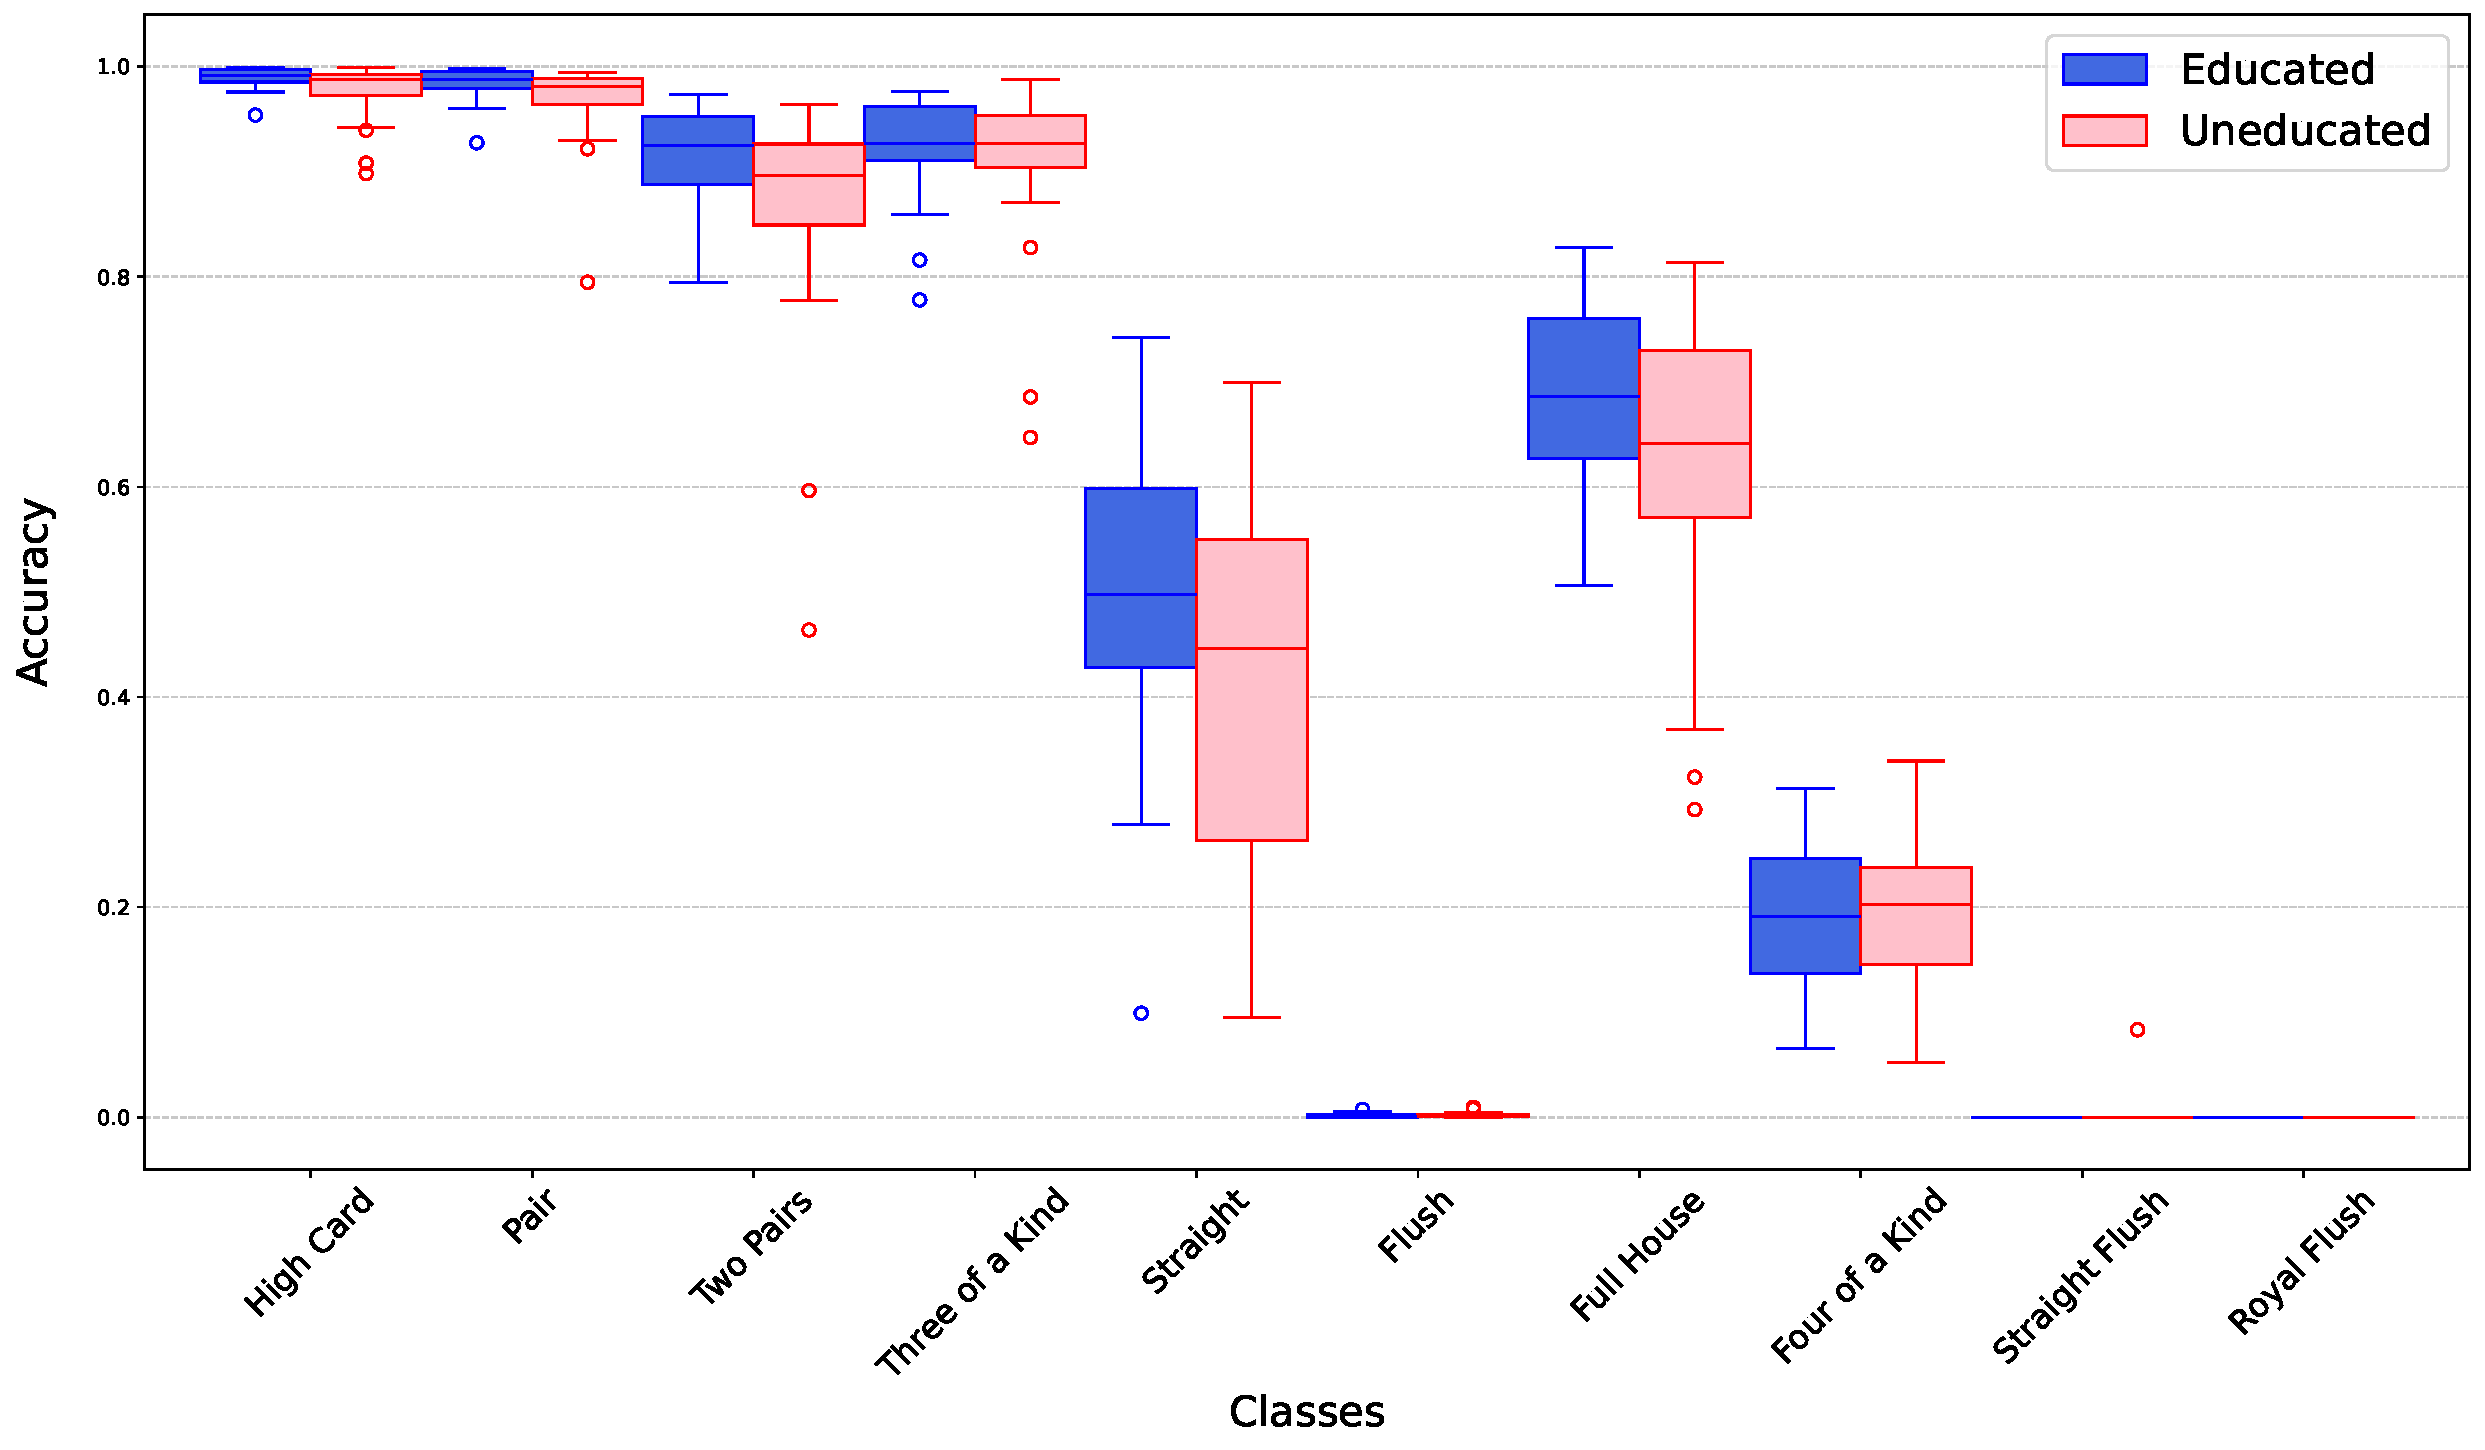
\includegraphics[width=\linewidth]{figures/phds-kill-results}
    \caption[PHDS KILL results]{
        Per class results of the experiments on the \gls{PHDS} dataset using \gls{KILL}.
        %
        The \gls{KILL} method outperforms the uneducated \gls{NN} in the prediction of almost all classes.
        %
        For all class prediction, the Wilcoxon signed-rank test has been applied to compare the two configurations.
        %
        With a p-value threshold of $0.05$, we reject the null hypothesis in the case of \emph{high card}, \emph{pair}, and \emph{straight} classes.
    }
    \label{fig:phds-kill-results}
\end{figure}
%
We define two different configurations for experiments:
%
\begin{inlinelist}
    %
    \item ``uneducated'', where we use the \gls{NN} described in \Cref{par:phds-methodology},
    %
    \item ``educated'', where we apply \gls{KILL} on the same network architecture.
    %
\end{inlinelist}
%
For both configurations we use the same hyperparameters and perform $30$ runs.
%
Results are reported in \Cref{tab:phds-kill-results} and in \Cref{fig:phds-kill-results}.
%
In general, experiments show that both predictors are very good at classifying frequent classes such as \emph{high card} and \emph{pair}.
%
Also for less frequent classes , \emph{two pairs} and \emph{three of a kind}, accuracy is still high.
%
The remaining six classes represent the $0.8\%$ of the training set and therefore much more difficult to correctly predict.
%
For \emph{full house} and \emph{straight}, accuracy has middle values, while for the remaining classes accuracy is pretty close to $0$.
%
All of this is quite expected due to the strong unbalance in the distribution of classes.
%
The only remarkable fact is that accuracy is extremely low for class \emph{flush} even if less frequent classes such as \emph{full house} and \emph{four of a kind} have higher accuracy.
%
We hypothesise that this happens because the vast majority of data consists in classes which depend only on the values of rank and therefore the network tends to consider it much more.
%
Indeed, only \emph{flush}, \emph{straight flush} and \emph{royal flush} (about the $0.26\%$ of the training set) depend on the values of suit.
%
Concerning the comparison between the \emph{uneducated} predictor -- with no additional knowledge -- and the \emph{educated} predictor -- obtained by applying KILL algorithm -- results show that the latter has higher performances with statistic significance.
%
The Wilcoxon signed-rank test~\cite{wilcoxon1945} has been applied to compare the two configurations on all the metrics reported in \Cref{tab:phds-kill-results}.
%
In particular, because of the unbalanced nature of the dataset, the test on macro-F1 and weighted-F1 metrics is more reliable than the test on accuracy.
%
The test shows that the \emph{educated} predictor is significantly better than the \emph{uneducated} one for the overall accuracy, macro-F1 and weighted-F1 metrics (with $p < 0.05$).
%
Also, the \emph{educated} predictor is significantly better than the \emph{uneducated} one for the single mean class accuracies, except for \emph{high card}, \emph{pair} and \emph{straight} classes.


\section{Knowledge injection via network structuring}\label{sec:ski-contribution-kins}

\section{Discussion and future direction}\label{sec:ski-discussion-and-future-direction}
%! Author = matteomagnini
%! Date = 05/03/25

%----------------------------------------------------------------------------------------
\chapter[Platform for symbolic knowledge injection]{\Glsentrylong{PSyKI}}
\label{ch:psyki}
\minitoc
%----------------------------------------------------------------------------------------

In this chapter, we present the \Gls{PSyKI} platform, which is a framework for \gls{SKI} methods.
%
\Gls{PSyKI} provides a unified way to implement \gls{SKI} methods, aiming to facilitate the development and comparison of different approaches.
%
It also provides a set of tools to evaluate the performance of \gls{SKI} methods, including metrics for measuring the quality of the injected knowledge and the performance of the resulting models.
%
In \Cref{sec:psyki}, we present the work ``\emph{On the Design of PSyKI: A Platform for Symbolic Knowledge Injection into Sub-symbolic Predictors}''~\cite{DBLP:conf/atal/MagniniCO22}, which describes the design and implementation of \gls{PSyKI}.
%
Then, in \Cref{sec:qos}, we present respectively two works that study the quality of service of \gls{SKI} methods:
%
in \Cref{sec:ski-meets-intelligent-agents} the paper ``\emph{Symbolic Knowledge Injection Meets Intelligent Agents}''~\cite{DBLP:journals/aamas/AgiolloRMCO23},
%
which introduces metrics for evaluating the performance of \gls{SKI} methods in the context of intelligent agents,
%
and in \Cref{sec:empirical-study-on-the-robustness-of-ski-methods} the paper ``\emph{An Empirical Study on the Robustness of Symbolic Knowledge Injection Techniques Against Data Degradation}''~\cite{DBLP:conf/woa/RafanelliMACO24},
%
which studies the robustness of \gls{SKI} methods against data degradation.


\section{PSyKI}\label{sec:psyki}
%
\Gls{PSyKI} is a (Python) platform for the development and evaluation of \gls{SKI} methods.
%
It is designed to provide a unified framework for implementing \gls{SKI} methods, allowing researchers and practitioners to easily develop, test, and compare different approaches.
%
In the following, we present a summary of the work ``\emph{On the Design of PSyKI: A Platform for Symbolic Knowledge Injection into Sub-symbolic Predictors}''~\cite{DBLP:conf/atal/MagniniCO22}, presented at the 4th International Workshop on EXplainable, Trustworthy, and Responsible AI and Multi-Agent Systems (EXTRAAMAS 2022)\footnote{\url{https://extraamas.ehealth.hevs.ch/archive.html}}.
%
The library is public available on GitLab and PyPi\footnote{\url{https://gitlab.com/psykei/psyki-python} and \url{https://pypi.org/project/psyki/}}.


\subsection{Motivations}\label{subsec:psyki-motivations}
%
This work is motivated by the need to address the common challenges that affect \gls{SKI} methods (see \Cref{subsec:limitations-and-challenges-of-ski}).
%
In particular, we want to address the following points:
%
\begin{inlinelist}
    \item \emph{lack of generality}, by providing the proper tools to automatically translate symbolic knowledge of arbitrary domains into a format suitable for injection into sub-symbolic predictors,
    %
    \item \emph{lack of reproducibility}, by providing a unified framework for implementing \gls{SKI} methods, allowing researchers to easily develop, test, and compare different approaches, and
    %
    \item \emph{lack of availability}, by encouraging the development of reusable software libraries for \gls{SKI} methods.
    %
\end{inlinelist}
%
Concerning the last point mentioned in \Cref{subsec:limitations-and-challenges-of-ski}, we identified in the logic language of stratified Datalog with negation a suitable candidate for the symbolic knowledge representation.
%
It is expressive enough to represent a wide range of symbolic knowledge, while being simple enough to be easily translated into a format suitable for injection into sub-symbolic predictors.


\subsection{Design}\label{subsec:design-and-implementation}
%
\begin{figure}
    \centering
    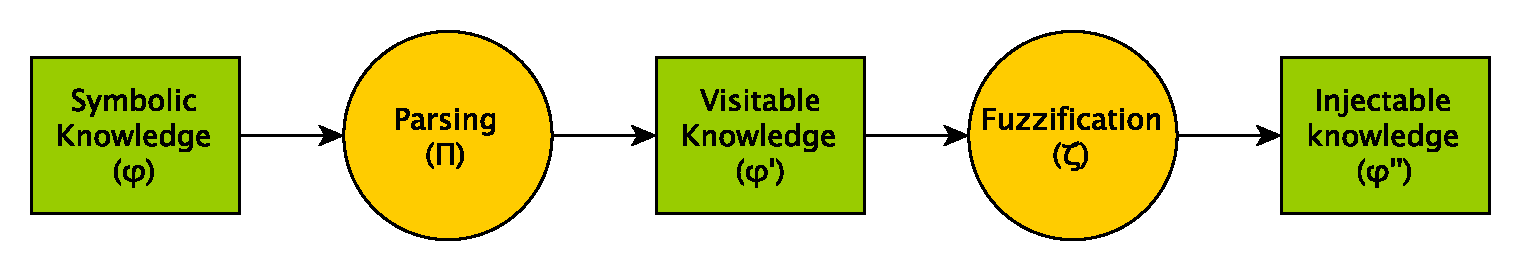
\includegraphics[width=\textwidth]{figures/knowledge-workflow-psyki}
    \caption[Symbolic knowledge transformation in PSyKI]{
        General workflow of symbolic knowledge transformation in \Gls{PSyKI}.
        The symbolic knowledge ($\phi$), typically expressed as logical formulas, is first parsed into a visitable form ($\phi'$), and then fuzzified into a machine-injectable representation ($\phi''$).
    }
    \label{fig:knowledge-workflow-psyki}
\end{figure}
%
All symbolic knowledge injection (\gls{SKI}) methods implemented in \gls{PSyKI} share a common transformation pipeline, illustrated in \Cref{fig:knowledge-workflow-psyki}.
%
Symbolic knowledge \(\phi\) cannot usually be injected directly into a sub-symbolic predictor.
%
Instead, it undergoes a two-step transformation:
%
\begin{inlinelist}
    %
    \item \emph{Parsing} (\(\Pi\)): the knowledge is converted into a visitable data structure, such as an \gls{AST} in the case of logic formulas, resulting in \(\phi'\);
    %
    \item \emph{Fuzzification} (\(\zeta\)): the parsed representation is transformed into a sub-symbolic form \(\phi''\), suitable for injection.
    %
\end{inlinelist}
%
Fuzzification plays a key role in bridging the symbolic and sub-symbolic domains.
%
It translates crisp Boolean logic into a form compatible with sub-symbolic models, often by relaxing discrete truth values into continuous-valued functions or generating neural components such as layers or entire \glspl{NN}.

\begin{figure}
    \centering
    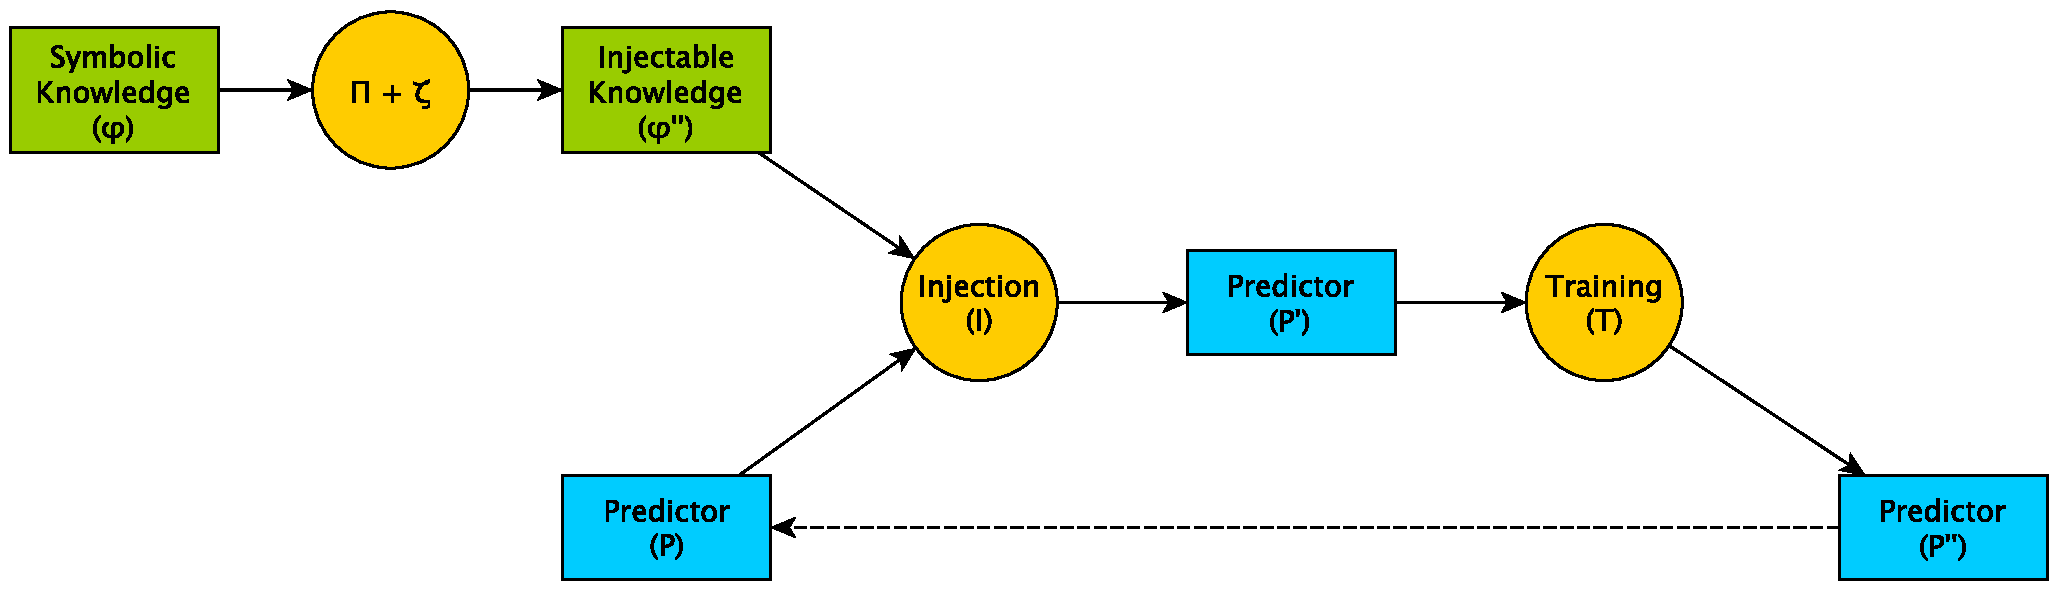
\includegraphics[width=\textwidth]{figures/psyki-workflow}
    \caption[General workflow of PSyKI]{
        Complete workflow of structuring and guided learning \gls{SKI} methods in \Gls{PSyKI}.
        The symbolic knowledge is transformed and injected into the sub-symbolic predictor, which is then trained on data.
    }
    \label{fig:psyki-workflow}
\end{figure}
%
\Cref{fig:psyki-workflow} shows the overall injection process in \gls{PSyKI}, including both the transformation of the symbolic knowledge and its integration into the learning system.
%
After the transformation phase, the different \gls{SKI} methods diverge:
%
\begin{inlinelist}
    %
    \item \emph{Structuring} and \emph{guided learning} inject \(\phi''\) directly into the architecture or training process of the predictor;
    %
    \item \emph{Embedding}-based methods use symbolic knowledge to enrich or generate the input data, so they are not directly represented in \Cref{fig:psyki-workflow}.
    %
\end{inlinelist}

\Gls{PSyKI} supports all three approaches, although it is primarily designed for \emph{structuring} and \emph{guided learning}, where the injection occurs directly into the predictor.
%
In general, \gls{SKI} algorithms operate on a predictor \(P\) and symbolic knowledge \(\phi\), producing a new predictor \(P'\) as output.
%
This modified predictor is then trained on data, resulting in a final model \(P''\), which can be reused in further iterations with different knowledge or injection strategies.


\paragraph{Architecture}\label{par:architecture}
%
\begin{figure}
    \centering
    \includegraphics[width=\textwidth]{figures/class-diagram}
    \caption[Class diagram of PSyKI]{
        Class diagram of \Gls{PSyKI}.
        %
        The main components are the \emph{Injector}, the \emph{Formula} and the \emph{Fuzzifier}.
        %
        The package \emph{logic.datalog} is an examplification showing two \emph{Injector} implementations and their relationships.
    }
    \label{fig:psyki-class-diagram}
\end{figure}
%
Essentially, \gls{PSyKI} is designed around the notion of injector.
%
An injector is any algorithm accepting a \gls{ML} predictor and prior symbolic knowledge -- predominantly logic formulas -- as input that produces a new predictor as output.
%
In order to properly perform injection, injectors may require additional information such as algorithm specific hyperparameters.


\gls{PSyKI} supports the processing of symbolic knowledge represented via logic formulas.
%
Based on the sort of logic, user can build an \gls{AST} for each formula.
%
The \gls{AST} can be inspected through a fuzzifier via pattern visitor to encode the symbolic knowledge to a sub-symbolic form (e.g. fuzzy logic functions, ad-hoc layers).
%
The resulting sub-symbolic object can finally be used by an injector to create a new predictor.
%
This process -- denoted with $\zeta$ \Cref{fig:psyki-workflow} -- is injector specific; instead, the same parser $\Pi$ can be used for logic formulas of the same sort independently of the injector.


The software is organized into well-separated packages to ensure easy extensibility towards new sort of logic and fuzzifiers---see \Cref{fig:psyki-class-diagram}
%
An \gls{AST} is a \emph{formula} object, and it can have different language specific elements w.r.t. the logic form that is covered.
%
Each formula implementation is self-contained inside a standalone package so that if a user wants to add a new logic form it is sufficient to add its implementation in a new package.
%
Similarly, a fuzzifier object that targets a specific logic form can be added inside the same package of the logic, there can be any number of fuzzifiers for a given logic.


\subsection{Implementation}\label{subsec:psyki-implementation}
%
\paragraph{Knowledge representation}\label{par:knowledge-representation}
%
\begin{figure}
    \centering
    \includegraphics[width=\textwidth]{figures/grammar}
    \caption[Class diagram for the representation of Datalog formulas]{
        A supported grammar of \Gls{PSyKI} for logic formulas.
        %
        The grammar is designed to represent Datalog formulas.
    }
    \label{fig:grammar}
\end{figure}
%
A crucial point in the \gls{SKI} workflow is the embedding of knowledge from symbolic into sub-symbolic form.
%
Ideally, there is no constraint on the formalism used to represent the prior knowledge (e.g., logic formulas, knowledge graph).
%
The most common knowledge representation form that \gls{SKI} algorithms claim to support is \gls{FOL} or one of its subsets.
%
However, there are characteristics of \gls{FOL} that are not ideal for some predictors.
%
Recursion and function symbols -- that allow recursive structures -- cannot be easily integrated into a predictor that is acyclic -- i.e., no recursive -- by construction such as conventional \gls{NN} (virtually all \gls{NN}, with few exceptions like fibred \gls{NN}~\cite{DBLP:conf/flairs/BaderGH05}).
%
Conversely, in this work we consider one of the most general and expressive logic formalism that does not support recursion and function symbols: stratified Datalog with negation.


Stratified Datalog with negation has been already described in detail in \Cref{subsec:ski-stratified-datalog-with-negation}.
%
To support injection into a particular predictor, we further assume the input knowledge base defines at least one outer relation -- say output or class -- involving as many variables as the input and output features the predictor has been trained upon.
%
Such a relation may be defined via one or more clauses, and each clause may leverage on other predicates in their bodies.
%
In turn, each predicate may be defined through one or more clause.
%
In that case, since we rely on stratified Datalog, we require input knowledge to not include any (directly or indirectly) recursive clause definition.


Once that the logic has been formalized, the implementation of a \emph{Formula} -- visitable data structure like an \gls{AST} -- is quite straightforward.
%
\Cref{fig:grammar} depicts the general API for representing logic formulas, as currently supported by \gls{PSyKI}.
%
To make \gls{PSyKI} able to parse bare text into actual logic formulas compliant to that API, we rely on well-established parser-generation facilities such as ANTLR~\cite{DBLP:journals/spe/ParrQ95}.
%
As further discussed below, the knowledge contained into a Formula object, can then be embedded in sub-symbolic form, via a fuzzifier, to be later injected into a predictor.


Later in the evolution of \gls{PSyKI} (i.e., from v. 0.2.1), we considered switching to a more established logic language for representing the symbolic knowledge: Prolog~\cite{DBLP:journals/tplp/KornerLBCDHMWDA22}.
%
In particular, we abandoned the manual parsing of logic formulas with ANTLR, and we rely on the tuProlog~\cite{DBLP:conf/padl/DentiOR01} framework.
%
We use the parser of tuProlog to parse the logic formulas, but \gls{PSyKI} does not support the full Prolog language because of the limitations of injecting into \gls{NN} mentioned in \Cref{subsec:limitations-and-challenges-of-ski} (i.e., we still support only stratified Datalog with negation).


\paragraph{Fuzzification}\label{par:fuzzification}
%
While logic formulas are commonly interpreted in a Boolean way -- i.e., they can be assigned with one truth value among true and false --, sub-symbolic predictors are more flexible-hence supporting formulas to hold up to some extent.
%
Switching from the former interpretation to the latter is, essentially, the purpose of fuzzifiers.
%
In practice, this implies converting a logic formula into a function of real numbers.
%
Along this line, fuzzification may be performed in (at least) two ways; real numbers may either represent
%
\begin{inlinelist}
    %
    \item a \emph{penalty} for the violation of a formula, or
    %
    \item the \emph{degree of truth} of that formula.
    %
\end{inlinelist}

To serve this purpose, one may rely on a multivalued interpretation of logic inspired to $\L$ukasiewicz's logic, where the value true is represented by 0 (resp. 1), while higher (resp. lower) values represent ``falsity''.
%
In particular, this approach may be useful to constrain a predictor during its training.
%
Examples of this fuzzification approach are \gls{KILL} (\Cref{subsec:kill-fuzzifier}) and \gls{KINS} (\Cref{subsec:kins-fuzzifier}).
%
\Cref{tab:kill-logic-formulae,tab:kins-logic-formulae} show the logic formulas encoding into real-valued functions for \gls{KILL} and \gls{KINS}, implementing \emph{penalty} and \emph{degree of truth} respectively.


\paragraph{Injection}\label{par:injection}
%
\lstinputlisting[
    basicstyle=\fontsize{8}{9.5}\ttfamily\selectfont,
    label=lst:psyki-injection,
    float,
    caption={General code snippet for the use of a \gls{SKI} method in the current version of \gls{PSyKI} (v. 0.4.3).},
    captionpos=b,
    language=Python,
]{listings/psyki-injection.py}
%
Knowledge injection is the central step in \gls{SKI}.
%
It is carried out by \emph{injectors}, i.e., objects wrapping a particular injection strategy.
%
Each injector is expected to accept one sub-symbolic predictors as input, other the logic formulas that should be injected into that predictor.
%
As part of its operation, the injector is in charge of producing a new predictor as output, of the same type as the one provided as input.
%
The new predictor is altered in such a way that it is consistent w.r.t. the provided logic formulas.


While the main architecture of \gls{PSyKI} has been maintained stable during the years, the implementation has been continuously improved.
%
The current version of \gls{PSyKI} (v. 0.4.3) is implemented in Python 3.9.13, with main dependencies being \texttt{tensorflow}, \texttt{2ppy}, \texttt{scikit-learn}, and \texttt{pandas}.
%
\Cref{lst:psyki-injection} shows a general code snippet for the use of a \gls{SKI} algorithm in \gls{PSyKI} (v. 0.4.3).


\section[SKI meets intelligent agents]{\Gls{SKI} meets intelligent agents}\label{sec:ski-meets-intelligent-agents}
%
In this and in the next section, we present two works that study the \gls{QoS} of \gls{SKI} methods.
%
\Gls{QoS} is a crucial aspect of any non-trivial systems, and it is particularly important for \gls{SKI} because the vast majority of the works in this field do not provide any evaluation but the performance of the resulting model.
%
Moreover, \gls{SKI} methods and the resulting educated models have many other dimensions that can be evaluated a part from the straight prediction performance.
%
The metrics introduced in these works have been implemented and integrated into \gls{PSyKI} from version 0.2.14 and later.


The work ``\emph{Symbolic Knowledge Injection Meets Intelligent Agents}''~\cite{DBLP:journals/aamas/AgiolloRMCO23}, published in the \emph{Autonomous Agents and Multi-Agent Systems} journal, presents a set of metrics for evaluating the performance of \gls{SKI} methods in the context of intelligent agents.
%
Here we present a summary of the work, including the motivations, the proposed metrics, and the evaluation of \gls{SKI} methods in terms of \gls{QoS}.


\subsection{Motivations}\label{subsec:ski-meets-intelligent-agents-motivations}
%
The current practice of assessing \gls{SKI} methods primarily focuses on measuring improvements in the predictive performance of an educated predictor \(\hat{N}\) over its uneducated counterpart \(N\).
%
However, predictive performance is not the only relevant benefit of \gls{SKI} that should be evaluated.

There are multiple aspects of \glspl{ML} predictors that can be influenced by \gls{SKI}, and for which specific metrics should be defined.
%
For instance, \gls{SKI} may impact the \emph{memory footprint}, \emph{latency}, \emph{data efficiency}, and \emph{energy consumption} of the predictors it is applied to.
%
Collectively, these properties contribute to what we refer to as the \emph{efficiency} of a predictor.

In this work, we consider the following efficiency properties:
%
\begin{properties}
    \item \textbf{Memory footprint}: the size of the predictor, typically measured in terms of the number of parameters or computational operations required.
    %
    \label{itm:memory-footprint}
    %
    \item \textbf{Latency}: the time required to perform a single inference.
    %
    \label{itm:latency}
    %
    \item \textbf{Data efficiency}: the amount of data required to train the predictor to achieve a certain level of performance.
    %
    \label{itm:data-efficiency}
    %
    \item \textbf{Energy consumption}: the energy required to train and/or run the predictor.
    %
    \label{itm:energy-consumption}
    %
    \item \textbf{Predictive performance}: standard metrics such as accuracy, F1-score, or mean squared error.
    %
    \label{itm:predictive-performance}
\end{properties}

For brevity, we refer to any function that measures one of these properties as an \emph{efficiency metric}.
%
These metrics quantify the improvement in a given property \(P\) of the uneducated predictor \(N\) when transformed into its educated counterpart \(\hat{N}\) through a \gls{SKI} mechanism.

The resulting efficiency scores can be influenced by several factors:
%
\begin{factors}
    %
    \item \textbf{Knowledge quality and coverage}:
    %
    The educated predictor \(\hat{N}\) is obtained by injecting symbolic knowledge \(K\).
    %
    Both \(N\) and \(\hat{N}\) are trained on the same dataset \(D\), which describes the learning task.
    %
    Key questions include:
    %
    \begin{inlinelist}
        \item Are \(K\) and \(D\) coherent?
        \item Does \(K\) cover situations exemplified in \(D\)?
        \item Is \(K\) consistent, coherent, and correct?
        \item Can the same be said for \(D\)?
    \end{inlinelist}
    %
    The answers to these questions significantly affect the efficiency scores, as they depend on the interplay between \(K\) and \(D\).
    %
    \label{itm:knowledge-quality-and-coverage}

    \item \textbf{Baseline quality}:
    %
    Both \(N\) and \(\hat{N}\) target the same learning task.
    %
    Questions to consider include:
    %
    \begin{inlinelist}
        \item Is \(N\) biased in a statistical sense?
        \item If so, can \(\hat{N}\) improve any efficiency metric \(P\)?
        \item Even if \(N\) is unbiased, is the selected injection mechanism \(\mathcal{I}\) suitable for \(N\)?
    \end{inlinelist}
    %
    These factors highlight the dependency of efficiency measures on the nature of \(N\) and the injection mechanism \(\mathcal{I}\).
    %
    \label{itm:baseline-quality}

    \item \textbf{Task at hand}:
    %
    The learning task determines the training dataset \(D\) and the test dataset \(T\).
    %
    The choice of \(T\) impacts the evaluation of both \(N\) and \(\hat{N}\), and consequently, the efficiency scores.
    %
    \label{itm:task-at-hand}
\end{factors}

In summary, efficiency metrics evaluate a \gls{SKI} method \(\mathcal{I}\) in a specific context defined by:
%
\begin{inlinelist}
    \item the symbolic knowledge \(K\),
    \item the predictor \(N\),
    \item the training dataset \(D\), and
    \item the test dataset \(T\).
\end{inlinelist}
%
Thus, any efficiency metric must be parametric with respect to \(K\), \(N\), \(D\), and \(T\).


\subsection{Metrics}\label{subsec:ski-meets-intelligent-agents-metrics}
%
In this section, we propose the implementation and formalization of metrics to evaluate the efficiency of \gls{SKI} methods.
%
Specifically, we introduce \emph{memory footprint}, \emph{latency}, \emph{energy consumption}, and \emph{data efficiency} as key performance indicators for assessing \gls{SKI}.
%
These metrics aim to quantify the computational resource usage of \gls{SKI} methods and provide insights into their design and optimization.
%
Our focus is on understanding how these metrics can guide the development of \gls{SKI}-based systems, particularly within the context of \glspl{MAS}.
%
An in-depth analysis of the trade-offs between performance and efficiency is crucial for the effective implementation of AI predictors in \glspl{MAS}.
%

\subsubsection{Memory footprint}\label{subsubsec:ski-meets-intelligent-agents-memory-footprint}
%
In the context of \glspl{MAS}, the importance of sub-symbolic predictors is growing as the field moves towards more efficient and sustainable \gls{AI}.
%
The increasing demand for \gls{AI} systems that can operate on resource-constrained devices, such as IoT and edge devices, has driven research into solutions requiring less memory and computational resources~\cite{DBLP:journals/tplp/KornerLBCDHMWDA22,shallow2deep-extraamas2021,nnconstrained-applsci11}.
%
Several metrics have been proposed to measure the memory footprint of \gls{AI} predictors, particularly sub-symbolic ones~\cite{Kang2018,wu2018shift,LiberisEurosys2021}.
%
For instance, the memory footprint of \glspl{NN} can be quantified by counting their parameters, \glspl{FLOP}, or \glspl{MAC}, which represent the operations required for a single inference~\cite{skiqs-woa2022,huang_condensenet_2018,cheng_msnet_2019}.
%
These metrics are effective for analyzing predictor complexity and computational efficiency.

%
\Gls{SKI} mechanisms can reduce the memory footprint of sub-symbolic predictors by injecting prior knowledge, thereby reducing the need for data-driven learning of complex concepts.
%
This reduction in learned concepts often translates to fewer parameters, \glspl{FLOP}, and \glspl{MAC}, resulting in a smaller memory footprint.
%
We define the memory footprint improvement score as the memory saved by the educated predictor \(\hat{N}\) compared to its uneducated counterpart \(N\):
%
\begin{equation}
    \label{eq:memory-footprint-improvement-score}
    \mu_{\Psi, K, N}(\mathcal{I}) = \Psi(N) - \Psi(\mathcal{I}(K, N)),
\end{equation}
%
where \(\mathcal{I}(K, N)\) (a.k.a., $\hat{N}$) represents the educated predictor obtained by injecting symbolic knowledge \(K\) into \(N\).

%
The improvement score depends on the quality and coverage of the input knowledge (\Cref{itm:knowledge-quality-and-coverage}) and the memory footprint of the input predictor (\Cref{itm:baseline-quality}).
%
Higher-quality knowledge reduces the memory requirements of the educated predictor.
%
Similarly, predictors with lower initial memory footprints exhibit smaller improvements.
%
It is important to note that the memory footprint of a \gls{NN} is task-independent, as it is a structural property of the network.

%
Finally, a negative score indicates that the educated predictor is more memory-intensive than the uneducated one, suggesting that the \gls{SKI} approach is ineffective in reducing memory usage.


\subsubsection{Energy consumption}\label{subsubsec:ski-meets-intelligent-agents-energy-consumption}
%
The relationship between \glspl{MAS} and energy consumption is multifaceted and critical.
%
To operate effectively in resource-constrained environments, \glspl{MAS} require \gls{AI} systems that minimize energy usage.
%
The distributed nature of \glspl{MAS}, combined with the increasing demand for scalable and power-efficient solutions, further emphasizes this need.
%
However, the dynamic and real-time requirements of many \glspl{MAS} applications often lead to high energy consumption due to computational and resource demands.
%
The complexity of \glspl{MAS}, with multiple agents and their interactions, adds another layer of difficulty, especially when processing large datasets or executing complex algorithms.
%
Thus, energy consumption becomes a crucial factor in the design and implementation of \gls{AI} systems within \glspl{MAS}.

%
Several strategies can address this challenge.
%
One approach involves using energy-efficient hardware, such as low-power processors, or adopting distributed and federated learning techniques to distribute computational loads across multiple devices~\cite{savazzi2021opportunities}.
%
Another approach focuses on optimizing algorithms and data structures to reduce the computational requirements of agents.
%
The integration of sub-symbolic predictors, which typically require fewer computational resources than symbolic \gls{AI} methods, can also significantly reduce energy consumption.
%
Additionally, techniques such as compression and optimization of sub-symbolic predictors can further enhance energy efficiency.

%
\gls{SKI} methods offer a promising opportunity to improve energy efficiency in \glspl{MAS}.
%
By introducing injection mechanisms into the data-driven pipeline of sub-symbolic training, \gls{SKI} reduces the computational complexity of training and running predictors.
%
This is achieved by leveraging prior knowledge, which complements the training data and simplifies the learning process.
%
As a result, it is essential to evaluate the extent to which \gls{SKI} mechanisms contribute to reducing the energy consumption of sub-symbolic predictors throughout their lifecycle.

%
To analyze energy consumption, we first define the lifecycle of \gls{AI} predictors, which includes the following stages:
%
\begin{enumerate}
    \item \textbf{Model definition}: Data scientists analyze the task and select suitable sub-symbolic predictors and hyperparameters.
    %
    \item \textbf{Model training}: The predictor's parameters are tuned using training data, where the size and dimensionality of the dataset impact energy consumption.
    %
    \item \textbf{Model testing}: The predictor is evaluated on a limited test set to ensure satisfactory performance.
    %
    \item \textbf{Model deployment}: The predictor is used for inference, with energy consumption depending on usage frequency and application lifespan.
\end{enumerate}

%
Among these stages, training and deployment are the most resource-intensive.
%
Training involves repeated executions and updates of the predictor, while deployment energy consumption depends on the frequency and duration of usage, which are often unpredictable.

%
We propose two metrics to measure energy consumption:
%
\begin{itemize}
    \item \textbf{Inference energy consumption}:
    %
    The average energy consumed by a predictor \(N\) for a single inference is defined as:
    %
    \begin{equation}
        \label{eq:inference-energy}
        \Upsilon^\mathsf{i}_{\upsilon}(N, T) = \frac{1}{\vert T \vert} \sum_{t \in T} \upsilon(N, t),
    \end{equation}
    %
    where \(\upsilon(N, t)\) measures the energy consumed by \(N\) during inference on a sample \(t\) from the test set \(T\).
    %
    \item \textbf{Training energy consumption}:
    %
    The average energy consumed during training is defined as:
    %
    \begin{equation}
        \label{eq:training-energy}
        \Upsilon^\mathsf{t}_{\upsilon, \gamma}(e, N, T) = \frac{\gamma(e, N, T)}{e \cdot \vert T \vert} -  \Upsilon^\mathsf{i}_\upsilon(N, T),
    \end{equation}
    %
    where \(e\) is the number of epochs, \(|T|\) is the size of the training set, and \(\gamma(e, N, T)\) estimates the total energy consumed during training, including inference costs.
\end{itemize}

%
The energy consumption improvement of a \gls{SKI} mechanism \(\mathcal{I}\) is defined as the energy saved by the educated predictor \(\hat{N} = \mathcal{I}(K, N)\) compared to the uneducated predictor \(N\).
%
We distinguish between improvements during inference and training:
%
\begin{align}
    \varepsilon^\mathsf{i}_{\upsilon, K, N, T}(\mathcal{I}) &= \Upsilon^\mathsf{i}_{\upsilon}(N, T) - \Upsilon^\mathsf{i}_{\upsilon}(\mathcal{I}(K, N), T)
    \\
    \varepsilon^\mathsf{t}_{\upsilon, \gamma, e, K, N, T}(\mathcal{I}) &= \Upsilon^\mathsf{t}_{\upsilon, \gamma}(e, N, T) - \Upsilon^\mathsf{t}_{\upsilon, \gamma}(e, \mathcal{I}(K, N), T)
\end{align}

%
These metrics depend on several factors:
%
\begin{itemize}
    \item \textbf{Input knowledge (\Cref{itm:knowledge-quality-and-coverage})}: Complex knowledge may increase training energy consumption but reduce inference energy.
    %
    \item \textbf{Baseline predictor (\Cref{itm:baseline-quality})}: Energy-hungry predictors are more likely to benefit from \gls{SKI}.
    %
    \item \textbf{Task at hand (\Cref{itm:task-at-hand})}: Task-specific datasets influence energy consumption improvements.
\end{itemize}

%
In summary, \gls{SKI} mechanisms have the potential to significantly reduce energy consumption in \glspl{MAS}, particularly during inference, while potentially increasing training energy costs.
%
These trade-offs must be carefully evaluated to optimize the overall efficiency of \gls{AI} systems.


\subsubsection{Latency}\label{subsubsec:ski-meets-intelligent-agents-latency}
%
Latency refers to the time required to generate a single prediction using a sub-symbolic predictor.
%
Low latency is crucial in real-world applications where timely responses are essential, such as in intelligent transportation~\cite{grigorescu_survey_2020} and e-health~\cite{esteva_deep_2021}.
%
In \glspl{MAS}, latency plays a significant role as collaboration between agents requires minimal computational delays~\cite{hou_consensus_2017}.
%
Additionally, tasks involving large datasets or complex algorithms, such as decision-making, can further increase latency, making it a critical efficiency measure.

%
\gls{SKI} methods can help reduce latency by incorporating symbolic representations, which simplify computations and reduce the complexity of the system.
%
This simplification can also aid in identifying the root causes of increased latency, making \gls{SKI} a valuable approach for improving computational efficiency.

%
Latency is typically measured as the average time required to generate predictions over a test dataset \(T\).
%
Formally, the latency of a predictor \(N\) is defined as:
%
\begin{equation}
    \label{eq:latency}
    \Lambda(N, T) = \frac{1}{\vert T \vert} \sum_{t \in T} \Theta(N, t),
\end{equation}
%
where \(\Theta(N, t)\) represents the time taken by \(N\) to generate a prediction for a sample \(t \in T\).

%
To evaluate the impact of \gls{SKI}, we define the latency gain $\lambda_{K, N, T}(\mathcal{I})$ as the difference in latency between the educated predictor \(\hat{N} = \mathcal{I}(K, N)\) and the uneducated predictor \(N\):
%
\begin{equation}
    \label{eq:latency-gain}
    \lambda_{K, N, T}(\mathcal{I}) = \frac{1}{\vert T \vert} \sum_{t \in T} \left( \Theta(N, t) - \Theta(\hat{N}, t) \right) = \Lambda(N, T) - \Lambda(\hat{N}, T),
\end{equation}
%
where \(\mathcal{I}(K, N)\) represents the \gls{SKI} mechanism injecting symbolic knowledge \(K\) into \(N\).

%
The latency gain depends on several factors:
%
\begin{itemize}
    \item \textbf{Input knowledge (\Cref{itm:knowledge-quality-and-coverage})}: Large or complex knowledge bases may increase latency due to additional computations, but they can also reduce inference time by simplifying the predictor's operations.
    %
    \item \textbf{Baseline predictor (\Cref{itm:baseline-quality})}: Predictors with higher initial latency are more likely to benefit from \gls{SKI}.
    %
    \item \textbf{Task at hand (\Cref{itm:task-at-hand})}: Task-specific datasets influence latency measurements, as different tasks may require varying levels of computational effort.
\end{itemize}

%
It is important to note that latency is not always directly proportional to the number of operations in the predictor.
%
Sparse or inefficient operations at the hardware level, as well as variations in input data complexity, can significantly affect latency~\cite{shumailov_sponge_2021}.
%
Thus, evaluating latency gain provides valuable insights into the computational efficiency of \gls{SKI} methods.


\subsubsection{Data efficiency}\label{subsubsec:ski-meets-intelligent-agents-data-efficiency}
%
Data-efficiency is a critical aspect of \glspl{MAS}, as these systems often generate and process substantial amounts of data.
%
Inefficient data management can lead to increased latency, reduced accuracy, and higher energy consumption, all of which negatively impact system performance.

%
Sub-symbolic predictors, which rely on data-driven training algorithms, offer significant flexibility and performance.
%
However, they require large amounts of data for training, resulting in increased storage and processing demands.
%
Moreover, the quality of the data, particularly its representativeness of the task, is crucial for effective learning.
%
These requirements make data collection time-consuming and potentially prone to subjectivity or uncertainty, as seen in applications like emotion recognition~\cite{deng_survey_2021}.

%
Recent research has focused on developing data-frugal predictors~\cite{sanchez_tinyml_2020}.
%
Among these, \gls{SKI} mechanisms play a significant role by leveraging \emph{a priori} knowledge to reduce the computational burden of learning.
%
Instead of learning all concepts from data, \gls{SKI} allows injecting prior knowledge into the predictor, potentially reducing the amount of data required to achieve acceptable performance levels.
%
In this sense, \gls{SKI} can be considered a data-efficiency mechanism.

%
To quantify the data-efficiency gain of a given \gls{SKI} mechanism \(\mathcal{I}\), we first define the \emph{data footprint} of a predictor \(N\).
%
The data footprint represents the amount of data required to train \(N\) to achieve a specific performance level.
%
Assuming \(N\) is trained on a dataset \(D\) with samples of varying dimensions, over \(e\) epochs, and achieves a performance score \(\pi(N, T)\) on a test set \(T\), the data footprint is defined as:
%
\begin{equation}
    \label{eq:data-footprint}
    \Delta_\pi(e, N, D, T) = \frac{e}{\pi(N, T)} \sum_{d \in D} \beta(d),
\end{equation}
%
where \(\beta(d)\) is the memory size (in bytes) of a single training sample \(d\).

%
The data-efficiency gain of a \gls{SKI} mechanism \(\mathcal{I}\) is then defined as the difference between the data footprints of the uneducated predictor \(N\) and the educated predictor \(\hat{N} = \mathcal{I}(K, N)\), trained on datasets \(D\) and \(D'\), respectively:
%
\begin{equation}
    \label{eq:data-efficiency-gain}
    \delta_{e, K, N, D, D', T}(\mathcal{I}) = \Delta_\pi(e, N, D, T) - \Delta_\pi(e, \mathcal{I}(K, N), D', T)
\end{equation}

%
To improve data-efficiency, one can reduce the size of the training dataset \(D'\), either by decreasing the number of samples or by reducing their dimensionality through compression.
%
Additionally, engineering the \gls{SKI} mechanism and the educated predictor can further enhance data-efficiency.
%
For instance, the input knowledge \(K\) can compensate for the reduced dataset size, as the gain depends on both the quality of \(K\) (\Cref{itm:knowledge-quality-and-coverage}) and the baseline predictor (\Cref{itm:baseline-quality}).
%
Predictors that are more data-hungry tend to exhibit higher data-efficiency gains.


\subsection{Validation}\label{subsec:ski-meets-intelligent-agents-validation}
%
The \gls{QoS} metrics are implemented as a set of classes that extend the \texttt{Metric} abstract class.
%
Each class corresponds to a specific metric and is responsible for computing its respective score.
%
The \texttt{Metric} class provides a unified interface for all metrics, ensuring consistency and ease of use.
%
Two main methods are available for computing metric values:
%
\begin{inlinelist}
    \item \texttt{compute\_during\_training}, which evaluates the metric during the training phase, and
    %
    \item \texttt{compute\_during\_inference}, which evaluates the metric after the predictors are trained.
\end{inlinelist}
%
Both methods accept predictors as input parameters and allow additional customization, such as specifying the training set or batch size.

%
The implemented metrics include:
%
\begin{enumerate}
    \item \textbf{Memory}: evaluates memory consumption efficiency, as defined in Equation~\eqref{eq:memory-footprint-improvement-score}.
    %
    \item \textbf{Energy}: measures energy consumption efficiency, as defined in Equation~\eqref{eq:training-energy}.
    %
    \item \textbf{Latency}: assesses latency efficiency, as defined in Equation~\eqref{eq:latency-gain}.
    %
    \item \textbf{Data Efficiency}: evaluates data efficiency, as defined in Equation~\eqref{eq:data-efficiency-gain}.
\end{enumerate}
%
These metrics are included in the \texttt{psyki.qos} package.
%
Notably, the metrics can be computed for any pair of predictors, whether they are educated or uneducated, enabling flexible comparisons.

%
To validate the proposed \gls{QoS} metrics, we conducted several experiments.
%
The experimental design is as follows:
%
\begin{enumerate}
    \item We selected three classification tasks from the literature, each associated with datasets of increasing cardinality.
    %
    \item For each task, we trained an uneducated neural predictor \(N\) on the dataset \(D\), using a train/test split.
    %
    Additionally, we selected a symbolic knowledge base \(K\) to inject into \(N\).
    %
    \item We applied \gls{SKI} using multiple injection techniques supported by \gls{PSyKI}, namely \gls{KBANN}, \gls{KINS}, and \gls{KILL}, resulting in educated predictors \(\hat{N}\).
    %
    \item Finally, we computed the \gls{QoS} metrics for each educated predictor \(\hat{N}\) and compared them with the uneducated predictor \(N\) in terms of data efficiency, energy consumption, memory footprint, latency, and accuracy variation.
\end{enumerate}
%
The goal of these experiments is to demonstrate the effectiveness of the \gls{QoS} metrics in evaluating the efficiency of different \gls{SKI} techniques.

%
It is important to note that these experiments are not intended as a comprehensive evaluation of \gls{SKI} techniques.
%
Instead, they aim to validate the proposed \gls{QoS} metrics by highlighting their ability to reveal variations in efficiency metrics introduced by \gls{SKI}.
%
Negative values in the results may reflect limitations in the injection algorithms or their implementation in \gls{PSyKI}.
%
The primary objective of \gls{PSyKI} is to provide correct, albeit not fully optimized, \gls{SKI} techniques.


\paragraph{Datasets}
%
We selected three datasets from the UCI\footnote{\url{https://archive.ics.uci.edu/}} repository: \gls{BCW}, \gls{PSJGS}, and \gls{CI}.
%
These datasets were chosen due to their varying cardinalities, ranging from \(10^2\) to \(10^4\), allowing us to evaluate the scalability and robustness of our predictors and metrics.

%
The \textbf{\glsfull{BCW}} dataset~\cite{breast_cancer_wisconsin_original_15} contains 699 instances of breast cancer biopsy results.
%
Each instance includes 9 features summarizing biological characteristics and one class label.
%
Feature values are integers in the range \([1, 10]\), and the \texttt{BareNuclei} feature has 16 missing values, which we replaced with 0.
%
The target variable is binary, indicating whether a biopsy is benign or malignant, with class distributions of 458 and 241, respectively.
%
The dataset is used to develop predictors for accurate breast cancer diagnosis based on biopsy features.

%
The \textbf{\glsfull{PSJGS}} dataset~\cite{splice-junction_gene_sequences_69} consists of 3,190 instances, each representing a sequence of 60 DNA nucleotides.
%
This dataset has been already introduced in this work in \Cref{subsec:kins-validation}.

%
The \textbf{\glsfull{CI}} dataset~\cite{census_income_20} contains 48,842 instances, each representing an individual from the 1994 United States Census.
%
Features include demographic and occupational information, and the target variable is binary, indicating whether an individual's annual income exceeds \(\$50,000\).
%
Class distributions are 37,155 for incomes less or equal to \(\$50,000\) and 11,687 for incomes greater than \(\$50,000\).
%
We converted the target variable to binary and removed irrelevant or biased features, such as \texttt{Fnlwgt} (similarity metric computed over the other features), \texttt{Education} (duplicated because of \texttt{EducationNumeric}), and \texttt{Race} (bias).
%
Remaining features were discretised, with \texttt{CapitalGain} and \texttt{CapitalLoss} binarised, and nominal categorical features one-hot encoded.

%
For all datasets, we divided the data into training and testing sets with a 2:3 ratio.
%
The knowledge bases for injection were obtained in a task-specific manner.
%
For the \gls{PSJGS} dataset, we used a knowledge base described in~\cite{DBLP:conf/aaai/TowellSN90}, converted into Prolog form.
%
For the \gls{BCW} and \gls{CI} datasets, we generated knowledge bases using a \gls{SKE} method~\cite{psyke-ia16}\footnote{more details about the knowledge extraction process is explained in the appendix of the original paper~\cite{DBLP:journals/aamas/AgiolloRMCO23}}.



\paragraph{Methodology}
%
For each dataset, we define and train several \glspl{NN}, including one uneducated network and multiple educated counterparts.
%
The educated networks are obtained by applying \gls{SKI} using the \gls{KINS}, \gls{KILL}, and \gls{KBANN} algorithms, each employing a distinct approach to knowledge injection.
%
This setup allows us to compare and evaluate the performance and efficiency metrics of the predictors.

%
For the uneducated predictors, we tune the structural hyperparameters, such as the number of layers and neurons per layer, using grid search with cross-validation.
%
The same process is applied to the educated predictors, except for those generated by \gls{KBANN}, where the architecture is determined by the input knowledge.
%
Specifically, we vary the number of layers (1 to 3) and the number of neurons per layer (10, 50, and 100) to ensure optimal hyperparameter selection while maintaining reasonable computation time.

%
To ensure statistical significance, we repeat the training process 30 times for each predictor, using different initial conditions and random seeds.
%
This approach reduces variability and provides a more accurate estimate of the predictors' average accuracy.
%
After computing the average accuracy, we evaluate the efficiency metrics for each predictor, including data-efficiency, energy consumption, memory footprint, and latency.
%
The results of this procedure are presented in \Cref{tab:qos-results}.


\subsection{Results and Discussion}\label{subsec:ski-meets-intelligent-agents-results-and-discussion}
%
\begin{table}
    \centering
    \begin{adjustbox}{width=\linewidth,center}
        \begin{tabular}{l|c|c|c|c|c|c|c}
            \toprule
            \textbf{Dataset} & \textbf{Model} & \textbf{Set} & \textbf{Data efficiency (KB)} & \textbf{Energy (mWh)} & \textbf{Memory (FLOPs)} & \textbf{Latency (ms)} & \textbf{Accuracy (\%
            )}\\
            \midrule
            % The table is devided into 3 macro rows, each devided into 4 macro rows, each devided into 2 rows (train and test):
            % 1. Breast Cancer
            % 1.1. uneducated
            % 1.2. KBANN
            % 1.3. KILL
            % 1.4. KINS
            % 2. Splice Junction
            % 2.1. uneducated
            % 2.2. KBANN
            % 2.3. KILL
            % 2.4. KINS
            % 3. Census Income
            % 3.1. uneducated
            % 3.2. KBANN
            % 3.3. KILL
            % 3.4. KINS
            \multirow{7}{*}{\textbf{BCW}} & \textbf{uneducated} & & -- & -- & -- & -- & 94.53\\
            \cmidrule{2-8}

            & \multirow{2}{*}{\textbf{KBANN}} & \textbf{train} & \multirow{2}{*}{35.89} & -1.47 & \multirow{2}{*}{3933} & \multirow{2}{*}{-1.70} & \multirow{2}{*}{95.45}\\
            & & \textbf{test} & & -0.10 & &  & \\
            \cline{2-8}

            & \multirow{2}{*}{\textbf{KILL}} & \textbf{train} & \multirow{2}{*}{4.09} & -0.99 & \multirow{2}{*}{0} & \multirow{2}{*}{0.35} & \multirow{2}{*}{94.63}\\
            & & \textbf{test} & & 0 & & &\\
            \cline{2-8}

            & \multirow{2}{*}{\textbf{KINS}} & \textbf{train} & \multirow{2}{*}{-9.97} & -1.22 & \multirow{2}{*}{-559} & \multirow{2}{*}{-1.41} & \multirow{2}{*}{94.29}\\
            & & \textbf{test} & & -0.09 & &  & \\
            \midrule


            \multirow{7}{*}{\textbf{PSJGS}} & \textbf{uneducated} & & -- & -- & -- & -- & 93.91\\
            \cline{2-8}
            & \multirow{2}{*}{\textbf{KBANN}} & \textbf{train} & \multirow{2}{*}{-4946.81} & -4.67 & \multirow{2}{*}{-66944} & \multirow{2}{*}{-2.56} & \multirow{2}{*}{92.84}\\
            & & \textbf{test} & & -0.22 & &  & \\
            \cline{2-8}
            & \multirow{2}{*}{\textbf{KILL}} & \textbf{train} & \multirow{2}{*}{553.89} & -3 & \multirow{2}{*}{0} & \multirow{2}{*}{0.04} & \multirow{2}{*}{94.02}\\
            & & \textbf{test} & & 0 & &  & \\
            \cline{2-8}
            & \multirow{2}{*}{\textbf{KINS}} & \textbf{train} & \multirow{2}{*}{-954.80} & -6.53 & \multirow{2}{*}{-161779} & \multirow{2}{*}{-4.75} & \multirow{2}{*}{93.70}\\
            & & \textbf{test} & & -0.51 & & & \\
            \midrule


            \multirow{7}{*}{\textbf{CI}} & \textbf{uneducated} & & -- & -- & -- & -- & 84.63\\
            \cline{2-8}
            & \multirow{2}{*}{\textbf{KBANN}} & \textbf{train} & \multirow{2}{*}{1653.79} & -1.41 & \multirow{2}{*}{-2468} & \multirow{2}{*}{-0.43} & \multirow{2}{*}{84.78}\\
            & & \textbf{test} & & -0.02 & & & \\
            \cline{2-8}
            & \multirow{2}{*}{\textbf{KILL}} & \textbf{train} & \multirow{2}{*}{4016.90} & -0.70 & \multirow{2}{*}{4200} & \multirow{2}{*}{0} & \multirow{2}{*}{84.81}\\
            & & \textbf{test} & & 0 & &  & \\
            \cline{2-8}
            & \multirow{2}{*}{\textbf{KINS}} & \textbf{train} & \multirow{2}{*}{4263.50} & -1.41 & \multirow{2}{*}{-6220} & \multirow{2}{*}{-0.44} & \multirow{2}{*}{84.77}\\
            & & \textbf{test} & & -0.02 & & & \\
            \bottomrule
        \end{tabular}
    \end{adjustbox}
    %
    \caption[QoS results for different \gls{SKI} methods]{
        %
        Comparison of the performance of different models after \gls{SKI} w.r.t. the uneducated one on the three datasets in terms data efficiency, energy consumption, memory usage, latency, and accuracy.
        %
        The values reported are the average of 30 runs for each model.
    }
    %
    \label{tab:qos-results}
\end{table}

%
Each column of \Cref{tab:qos-results} is examined to provide insights into the performance of the predictors.
%
The \emph{data-efficiency} scores vary significantly across predictors and datasets.
%
A positive score indicates that the educated predictor is more efficient than its uneducated counterpart, while a negative score suggests the opposite.
%
This variation highlights the importance of selecting the most suitable predictor for a given task.
%
For instance, the \gls{KINS}-based solution shows lower data-efficiency scores on the \gls{BCW} dataset compared to other predictors, suggesting it may not be the best choice for this task.
%
Conversely, all three predictors exhibit positive data-efficiency scores on the \gls{CI} dataset, indicating improvements across all \gls{SKI} algorithms.


The \emph{energy consumption} metrics, shown in the second column, are mostly negative for both training and testing phases.
%
This indicates that educated predictors often consume more energy than uneducated ones.
%
For example, the \gls{KBANN}-based solution generally requires more energy, while the \gls{KILL}-based solution is more energy-efficient.
%
The complexity of the input knowledge can significantly impact energy consumption, particularly during training.
%
Complex knowledge may improve data efficiency but at the cost of higher energy requirements.

%
The \emph{memory footprint} results, presented in the third column, reveal mixed outcomes.
%
A positive value indicates reduced memory usage by the educated predictor, while a negative value suggests increased memory consumption.
%
For instance, the \gls{KBANN}-based solution reduces memory usage on the \gls{BCW} dataset but increases it on the \gls{PSJGS} dataset.
%
The \gls{KILL}-based solution often shows no difference in memory usage, with a metric value of zero.

%
The \emph{latency} results, shown in the fourth column, compare the time required for inference between educated and uneducated predictors.
%
The \gls{KILL}-based solution exhibits similar latency to its uneducated counterpart, with metrics close to zero.
%
However, the \gls{KBANN} and \gls{KINS}-based solutions show slightly higher latency across all datasets.
%
This increase is likely due to the complexity of the injected knowledge.

%
Finally, the \emph{accuracy} scores, presented in the last column, indicate that both educated and uneducated predictors perform similarly across all datasets.
%
This suggests that the predictors are capable of achieving consistent and accurate results regardless of the injection mechanism.

%
In summary, educated predictors generally require fewer data to achieve similar accuracy, making them advantageous in resource-constrained settings.
%
However, they may incur higher energy and latency costs, depending on the complexity of the injected knowledge.
%
The memory usage varies, with some predictors showing improvements and others not.
%
These findings emphasize the importance of using specific metrics beyond accuracy to evaluate \gls{SKI} methods.

%
In this work, we propose a set of \gls{QoS} metrics to evaluate \gls{SKI} mechanisms, focusing on efficiency gains.
%
The metrics include \emph{memory footprint efficiency}, \emph{energy efficiency}, \emph{latency efficiency}, and \emph{data efficiency}.
%
To support their practical application, we extend the \gls{PSyKI} library with a general-purpose implementation of these metrics.

%
Our experiments demonstrate that these metrics provide valuable insights into the efficiency of \gls{SKI} mechanisms.
%
For instance, they reveal whether a given mechanism improves a predictor's efficiency according to specific criteria.
%
Additionally, the results highlight areas for improvement in the current \gls{PSyKI} injection mechanisms.

%
In the context of \glspl{MAS}, these metrics address challenges such as energy consumption, latency, memory, and data efficiency.
%
By reducing computational requirements and improving data quality, \gls{SKI} approaches can enhance the performance and efficiency of intelligent systems.
%
Measuring efficiency gains enables the automation of decision-making processes, allowing agents to dynamically optimize their sub-symbolic components to achieve their goals.


\section[Empirical study on the robustness of SKI methods]{Empirical study on the robustness of \Gls{SKI} methods}\label{sec:empirical-study-on-the-robustness-of-ski-methods}
%
Here we present the work \emph{``An Empirical Study on the Robustness of Knowledge Injection Techniques Against Data Degradation''}~\cite{DBLP:conf/woa/RafanelliMACO24}, presented at the 25th Workshop ``From Objects to Agents'' (WOA 2024)\footnote{\url{https://www.univda.it/woa2024/}}.
%
With this work, we extend the \gls{QoS} metrics introduced in \Cref{sec:ski-meets-intelligent-agents} to evaluate the robustness of \gls{SKI} methods.


\subsection{Motivations}\label{subsec:empirical-study-on-the-robustness-of-ski-methods-motivations}
%
Robustness is a critical challenge for \glspl{NN}~\cite{placeholder}, referring to their ability to maintain performance despite input perturbations.
%
In general, a more robust neural network produces more reliable and accurate predictions.

%
Several techniques have been proposed to enhance the robustness of \glspl{NN}, including regularization~\cite{placeholder}, data augmentation~\cite{placeholder}, and adversarial training~\cite{placeholder}.
%
The interest in robustness stems from two main factors:
%
\begin{enumerate}
    \item The need to address limitations of \glspl{NN}, such as their sensitivity to random perturbations~\cite{placeholder}.
    %
    \item The growing focus on \emph{trustworthy AI} (\gls{TAI}), which emphasizes transparency, responsibility, ethics, and safety in \gls{AI} systems~\cite{placeholder}.
\end{enumerate}

%
\Gls{TAI} has gained significant attention due to the increasing adoption of \gls{AI} and the interest of policymakers, as reflected in guidelines such as those from the European Union~\cite{placeholder}.
%
Robustness is a key component of \gls{TAI}, ensuring that \gls{AI} systems function consistently and accurately across diverse scenarios.
%
In this context, research on \gls{NN} trustworthiness has advanced significantly, with neuro-symbolic methods emerging as a promising approach.

%
Neuro-symbolic methods~\cite{placeholder} aim to combine the strengths of \glspl{NN} and symbolic \gls{AI}, addressing their respective weaknesses, such as the opacity of \glspl{NN} and the limited scalability of symbolic systems.
%
These methods can enhance \gls{NN} robustness by incorporating symbolic knowledge, which is typically represented as facts and rules in logic form.
%
Symbolic knowledge provides a structured and often intensional representation, which is particularly useful in scenarios where training data is noisy or incomplete.
%
By leveraging concise yet general logic rules, symbolic knowledge can compensate for missing or low-quality data, improving the performance of \glspl{NN} even under challenging conditions.

%
This work focuses on \emph{symbolic knowledge injection} (\gls{SKI}) as a neuro-symbolic integration approach.
%
\Gls{SKI} involves algorithmic procedures that modify sub-symbolic predictors to ensure their predictions are consistent with given symbolic knowledge.
%
The injected knowledge can take various forms, such as logical rules, knowledge graphs, or expert knowledge~\cite{placeholder}.
%
Common \gls{SKI} methods include constraining-based and structuring-based approaches, while embedding symbolic knowledge directly into \glspl{NN} is beyond the scope of this study.

%
Formally, we denote an injection procedure as:
%
\begin{equation}
    \hat{N} = \mathcal{I}(N, K, D),
\end{equation}
%
where \(N\) is the uneducated predictor, \(K\) is the symbolic knowledge, \(D\) is the training dataset, \(\mathcal{I}\) is the injection mechanism, and \(\hat{N}\) is the educated predictor.
%
For simplicity, we refer to \(\hat{N}\) as the educated predictor and \(N\) as the uneducated one.

%
The effectiveness of \gls{SKI} is typically measured by the performance gain of the educated predictor \(\hat{N}\) compared to its uneducated counterpart \(N\), using metrics such as accuracy, F1-score, or mean squared error.
%
However, these metrics primarily assess predictive performance and do not capture the robustness of the injection mechanism.
%
To address this gap, this work introduces a metric to evaluate the robustness of \gls{SKI} mechanisms relative to their uneducated counterparts.


\subsection{Robustness of \gls{SKI} Methods}\label{subsec:empirical-study-on-the-robustness-of-ski-methods-robustness-of-ski-methods}
%
In counterfactual analysis~\cite{placeholder}, controlled perturbations of training data are commonly used to evaluate the robustness of predictors.
%
Inspired by this approach, we define the \emph{statistical robustness} of a \gls{SKI} procedure.
%
An injection mechanism is considered robust if the predictive performance of the educated predictor is minimally affected by small perturbations in the training data.
%
This section provides an overview of robustness, detailing the types of perturbations applicable to training data and how their magnitude can be quantified.
%
We define a data perturbation as a modification of a training dataset \(D\) by adding, removing, or editing its entries.
%
The perturbed dataset is denoted as \(D' = D \circ \Delta D\), where \(\circ\) represents the perturbation operator.
%
The magnitude of the perturbation, \(\|\Delta D\|\), is a non-negative scalar quantifying the extent of changes introduced.
%
Let \(\mathcal{D} = \{\Delta D_1, \ldots, \Delta D_n\}\) be a set of perturbations applied to \(D\).
%
Let \(N\) be a predictor trained on \(D\), and \(N_{\Delta D}\) be the predictor trained on the perturbed dataset \(D \circ \Delta D\), with the same hyperparameters as \(N\).
%
The robustness score of \(N\) with respect to \(\mathcal{D}\) is defined as:
%
\begin{equation}
    \label{eq:memory-footprint-improvement-score}
    \rho_{N, D}(\mathcal{D}) = \frac{1}{n} \sum_{\Delta D \in \mathcal{D}} \|\Delta D\| \cdot \frac{\pi(N_{\Delta D}, D \circ \Delta D)}{\pi(N, D)},
\end{equation}
%
where \(\pi\) is a performance metric, such as accuracy, computed on the respective dataset.
%
Robustness is proportional to the magnitude of perturbations and the ratio of the performance of the perturbed predictor to the unperturbed one.
%
Although all components in Equation~\eqref{eq:memory-footprint-improvement-score} are positive, not all perturbations improve performance.
%
The performance ratio can exceed 1 when the perturbed model performs better, indicating a positive perturbation.
%
Conversely, it falls below 1 when the perturbed model performs worse, indicating a negative perturbation.
%
A robust predictor exhibits minimal performance degradation under significant perturbations, implying that its robustness increases as the impact of perturbations decreases.
%
The robustness of an injection mechanism can be evaluated by applying Equation~\eqref{eq:memory-footprint-improvement-score} to an educated predictor \(\hat{N} = \mathcal{I}(N, K, D)\), where \(\mathcal{I}\) is the injection mechanism and \(K\) is the symbolic knowledge.
%
The robustness gain score is defined as:
%
\begin{equation}
    \label{eq:robustness-gain}
    R_{N, D}(\mathcal{I}) = \frac{\rho_{\hat{N}, D}(\mathcal{D})}{\rho_{N, D}(\mathcal{D})}.
\end{equation}
%
A robustness gain \(R_{N, D}(\mathcal{I}) > 1\) indicates that the injection mechanism improves robustness compared to the uneducated predictor.
%
Conversely, \(R_{N, D}(\mathcal{I}) < 1\) suggests that the educated predictor is less robust under data perturbations.
%
This metric provides an intuitive measure for analyzing the robustness of \gls{SKI} mechanisms.


\subsubsection{Perturbation Strategies}\label{subsubsec:perturbation-strategies}
%
This section discusses three primary strategies for perturbing datasets: \emph{sample drop}, \emph{noise addition}, and \emph{label flipping}.
%
These strategies simulate common issues that degrade dataset quality, such as missing data, sensor noise, and mislabeling.

%
\paragraph{Sample Drop}
%
The \emph{sample drop} strategy models scenarios where an intelligent agent has limited access to training data.
%
This approach is often used to evaluate the effectiveness of neuro-symbolic methods in handling data scarcity~\cite{placeholder}.
%
The process involves randomly removing samples from a dataset \(D\) to produce a perturbed dataset \(D'\).
%
The removal is controlled by a \emph{dropping probability} \(p \in (0, 1)\), which is shared across all data entries in \(D\).
%
Formally, \(p = \mathbb{E}[X_d]\), where \(X_d \sim \mathcal{B}(p)\) is a Bernoulli random variable indicating whether a data entry \(d \in D\) is included (\(X_d = 1\)) or excluded (\(X_d = 0\)) in \(D'\).
%
Under these assumptions, the perturbed dataset is defined as:
%
\[
D' = \{d \mid d \in D \text{ and } X_d = 1\}.
\]
%
To construct a set of perturbations \(\mathcal{D} = \{\Delta D_1, \ldots, \Delta D_n\}\), the sample drop process is applied \(n\) times with increasing dropping probabilities \(0 < p_1 < \ldots < p_n < 1\).

%
\paragraph{Noise Addition}
%
The \emph{noise addition} strategy simulates errors in the data acquisition process, such as sensor noise, to evaluate the robustness of neuro-symbolic methods against unreliable data~\cite{placeholder}.
%
This involves adding random noise to the entries of \(D\) to produce a perturbed dataset \(D'\).
%
The process is controlled by a \emph{noise intensity} \(v \geq 0\), which determines the covariance matrix of the noise.
%
Specifically, the noise is modeled as a zero-mean, multivariate normal random variable \(V_d \sim \mathcal{N}(0, v \cdot I)\), where \(I\) is the identity matrix.
%
The perturbed dataset is then defined as:
%
\[
D' = \{d + V_d \mid d \in D\}.
\]
%
The number of samples remains unchanged, i.e., \(|D| = |D'|\).
%
To construct a set of perturbations \(\mathcal{D} = \{\Delta D_1, \ldots, \Delta D_n\}\), the noise addition process is applied \(n\) times with increasing noise intensities \(0 < v_1 < \ldots < v_n\).

%
\paragraph{Handling Discrete Features}
%
For datasets with ordinal or categorical features, the noise addition process must account for discontinuities.
%
In such cases, the normal noise distribution \(\mathcal{N}(0, v \cdot I)\) is replaced with its discrete counterpart~\cite{placeholder}.
%
For ordinal features, the noise is more likely to select values close to the original.
%
For categorical features, the noise selects values uniformly, similar to the label flipping strategy described below.

%
\paragraph{Label Flipping}
%
The \emph{label flipping} strategy models errors in the labeling process, such as human mislabeling, and is primarily applicable to classification tasks~\cite{placeholder}.
%
This involves randomly altering the output labels of data entries in \(D\) to produce a perturbed dataset \(D'\).
%
Assume the dataset has a single output feature with \(K\) possible classes.
%
For a data entry \(d = (x_{d,1}, \ldots, x_{d,m-1}, y_d) \in D\), where \(x_{d,j}\) are input features and \(y_d \in \{1, \ldots, K\}\) is the output label, the flipping process is controlled by a \emph{flipping probability} \(f \in (0, 1)\).
%
The new label \(Y_d\) is defined as:
%
\[
P(Y_d = k) =
\begin{cases}
f / (K - 1), & \text{if } k \neq y_d, \\
1 - f, & \text{if } k = y_d.
\end{cases}
\]
%
Thus, the perturbed dataset is:
%
\[
D' = \{(x_{d,1}, \ldots, x_{d,m-1}, y'_d) \mid d \in D \text{ and } Y_d = y'_d\}.
\]
%
To construct a set of perturbations \(\mathcal{D} = \{\Delta D_1, \ldots, \Delta D_n\}\), the label flipping process is applied \(n\) times with increasing flipping probabilities \(0 < f_1 < \ldots < f_n < 1\).

%
\paragraph{Applicability to Regression Problems}
%
Label flipping is not directly applicable to regression tasks, as the output features are continuous.
%
In such cases, label flipping can be modeled as a specific form of noise addition applied only to the output features.
%
However, this extension is beyond the scope of this work.


\subsection{Validation}\label{subsec:empirical-study-on-the-robustness-of-ski-methods-validation}
%
In this section, we describe the experimental setup and results used to evaluate the proposed robustness metric.
%
For reproducibility, the source code of the experiments is publicly available.\footnote{Add link or reference here.}
%
We use the same three datasets as in \Cref{subsec:ski-meets-intelligent-agents-validation}:
%
These datasets were selected for their varying characteristics, allowing a comprehensive evaluation of the robustness metric.

%
\paragraph{Injected Knowledge}
%
For each dataset, we use symbolic knowledge in Prolog syntax to define classification rules.
%
The \gls{PSJGS} dataset uses a knowledge base from the literature~\cite{placeholder}, with an additional rule to classify the \texttt{none} class:
%
\[
\texttt{class}(\bar{X}, \texttt{n}) \leftarrow \neg \texttt{class}(\bar{X}, \texttt{ei}) \land \neg \texttt{class}(\bar{X}, \texttt{ie}),
\]
%
where \(\bar{X}\) represents the sequence of variables corresponding to the DNA sequence.
%
For the \gls{BCW} and \gls{CI} datasets, we define custom logic rules due to the lack of predefined knowledge bases.

%
\paragraph{Injectors}
%
We use the \gls{PSyKI} framework to apply three \gls{SKI} algorithms:
%
\begin{itemize}
    \item \textbf{\gls{KINS}}: A structuring-based mechanism that extends a neural network with additional modules to mimic symbolic knowledge~\cite{placeholder}.
    %
    \item \textbf{\gls{KILL}}: A guided-learning approach that adds a penalty term to the loss function during training to enforce compliance with symbolic knowledge~\cite{placeholder}.
    %
    \item \textbf{\gls{KBANN}}: A structuring-based method that constructs a neural network entirely from propositional rules~\cite{placeholder}.
\end{itemize}

%
\paragraph{Experimental Setup}
%
For each dataset, we train an uneducated model and apply the three injectors using the corresponding knowledge base.
%
The uneducated model consists of two hidden layers, one input layer, and one output layer, with \texttt{ReLU} activation functions and a \texttt{softmax} output layer.
%
The number of neurons per hidden layer is dataset-specific: [16, 8] for \gls{BCW}, [32, 16] for \gls{CI}, and [64, 32] for \gls{PSJGS}.
%
Training uses the categorical cross-entropy loss function, a batch size of 32, and a maximum of 100 epochs.

%
\paragraph{Data Perturbation}
%
We apply three perturbation strategies: \emph{sample drop}, \emph{noise addition}, and \emph{label flipping}.
%
The \emph{drop probability} \(d\) varies from 0.0 to 0.95 in steps of 0.05.
%
The \emph{flipping probability} \(f\) varies from 0.0 to 0.90 in steps of 0.08.
%
The \emph{noise intensity} \(v\) varies from 0.0 to 1.0 in steps of 0.1.
%
Each experiment is repeated 30 times to ensure statistical significance.

%
\paragraph{Robustness Metric}
%
Our analysis focuses exclusively on \gls{SKI} approaches, as no existing metrics directly evaluate training robustness.
%
The only related metric~\cite{placeholder} measures generalization capability.
%
Thus, we aim to validate the proposed robustness metric by assessing its ability to identify robust \gls{SKI} mechanisms.


\subsection{Results and Discussion}\label{subsec:empirical-study-on-the-robustness-of-ski-methods-results-and-discussion}
%
% !TeX root = ../phd-thesis.tex

\newcommand{\cellsize}{0.3\linewidth}

\begin{figure*}%[!h]
	\centering
	\begin{subfigure}{\cellsize}
		\caption{}
		\label{fig:bcw-drop}
		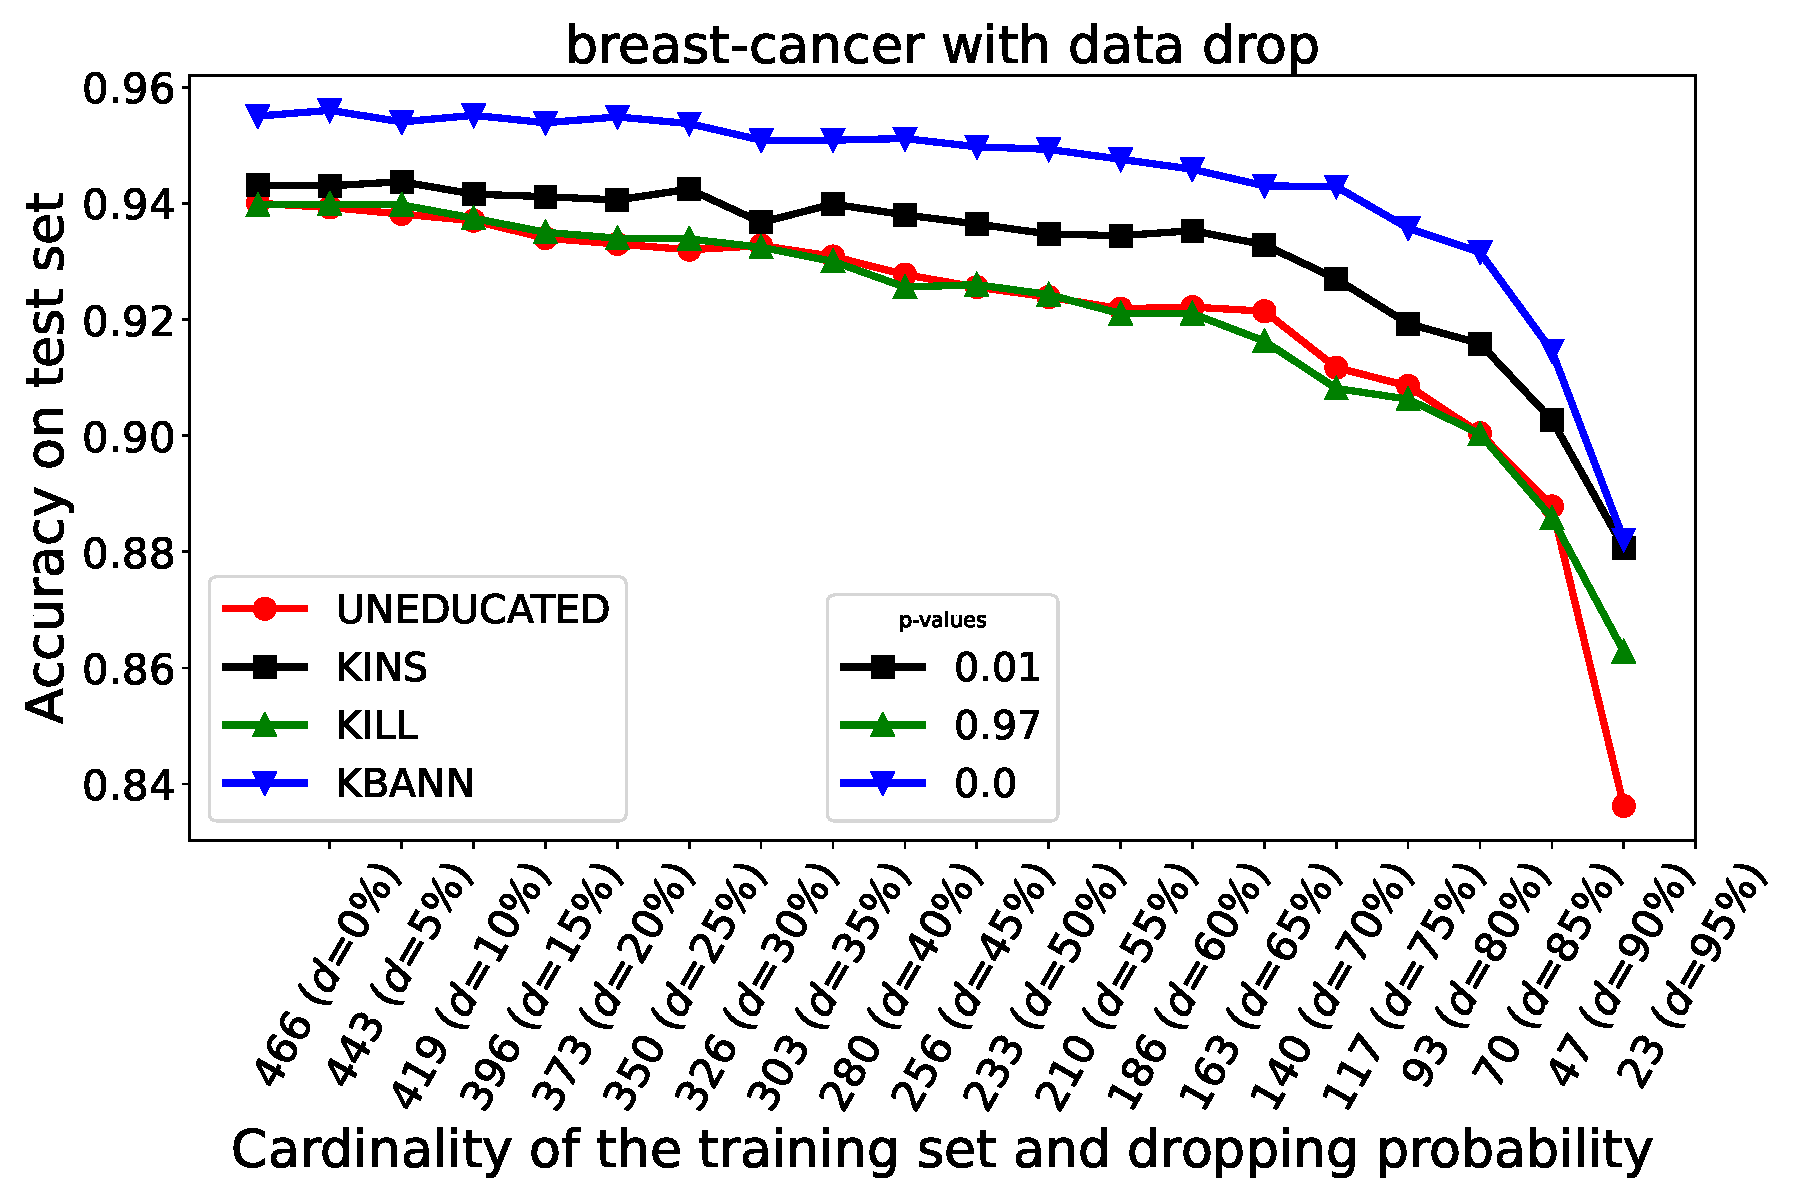
\includegraphics[width=\linewidth]{figures/drop/breast-cancer/uneducated-kins-kill-kbann-accuracy-average-curves}
	\end{subfigure}\hfil
	\begin{subfigure}{\cellsize}
		\caption{}
		\label{fig:psjgs-drop}
		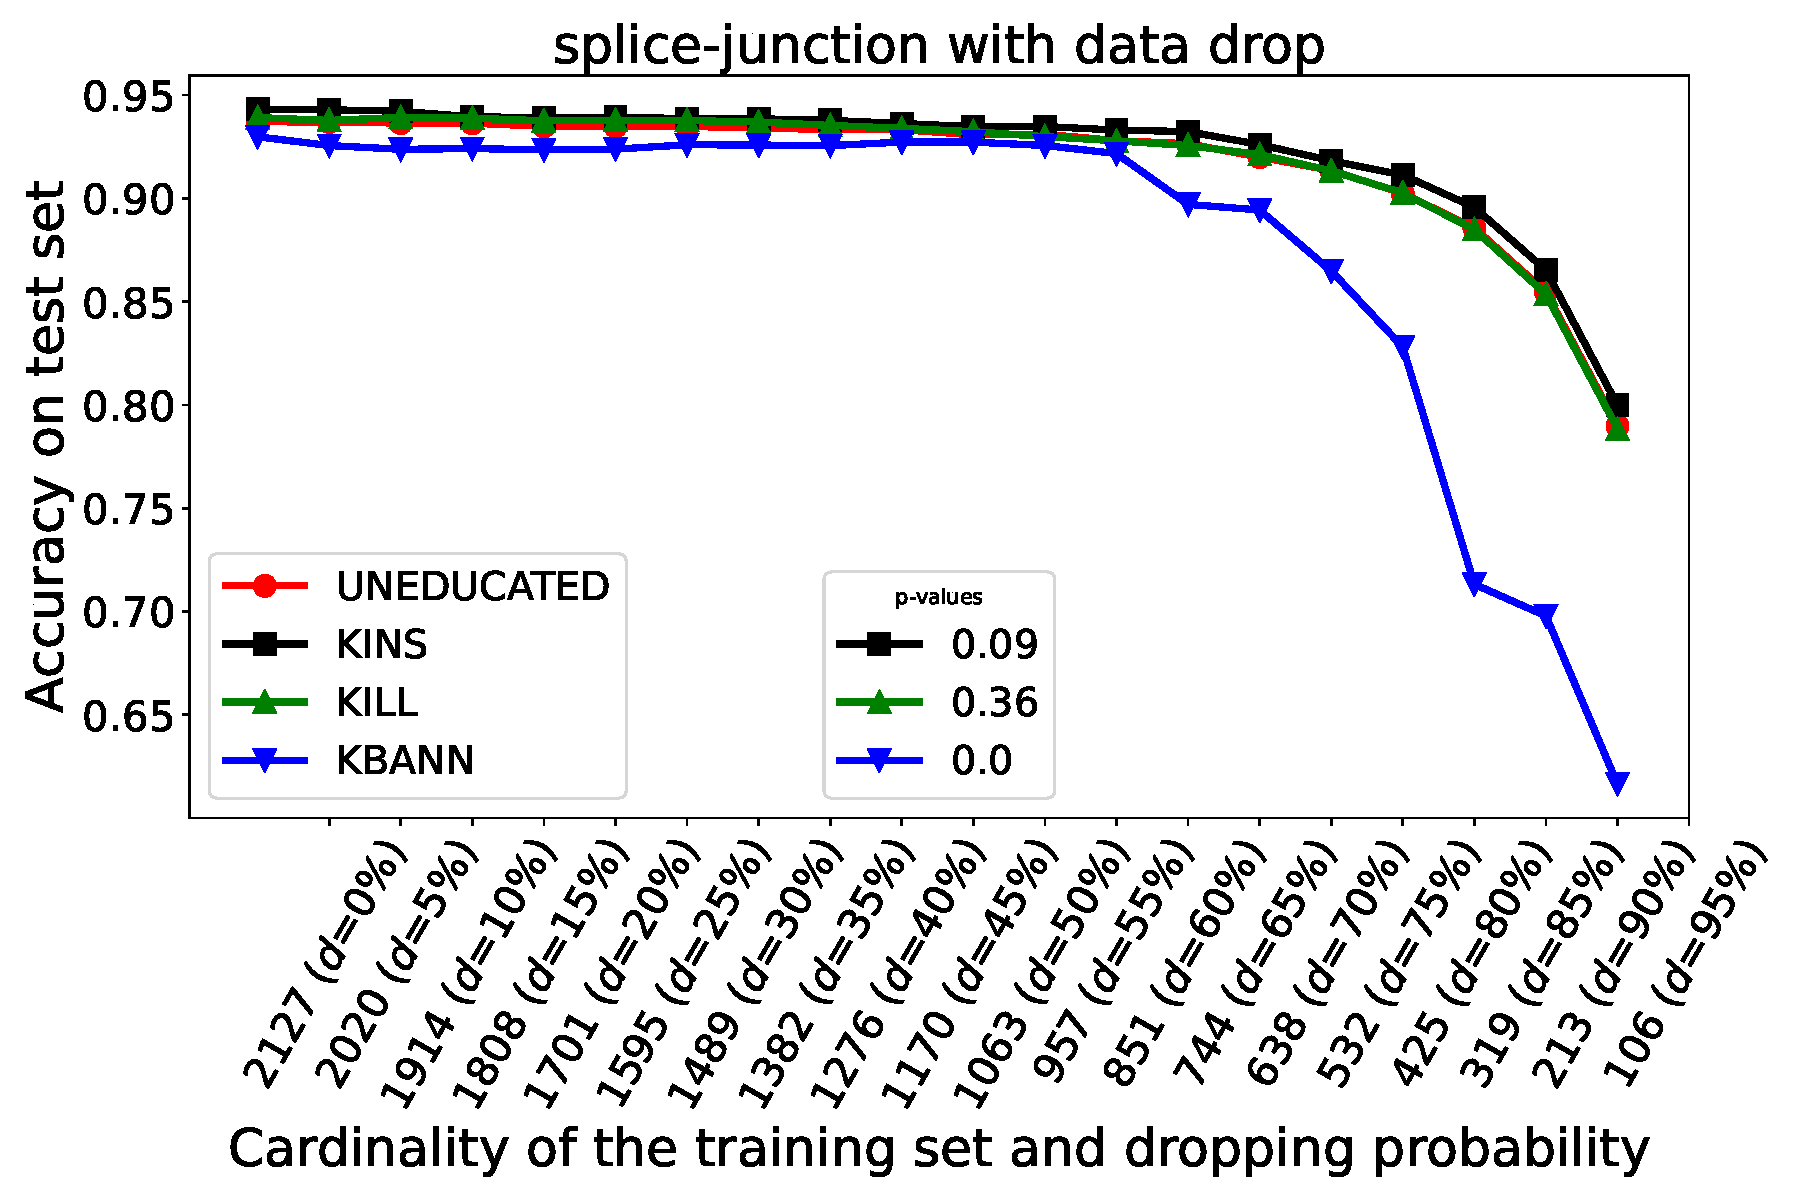
\includegraphics[width=\linewidth]{figures/drop/splice-junction/uneducated-kins-kill-kbann-accuracy-average-curves}
	\end{subfigure}\hfil
	\begin{subfigure}{\cellsize}
		\caption{}
		\label{fig:ci-drop}
		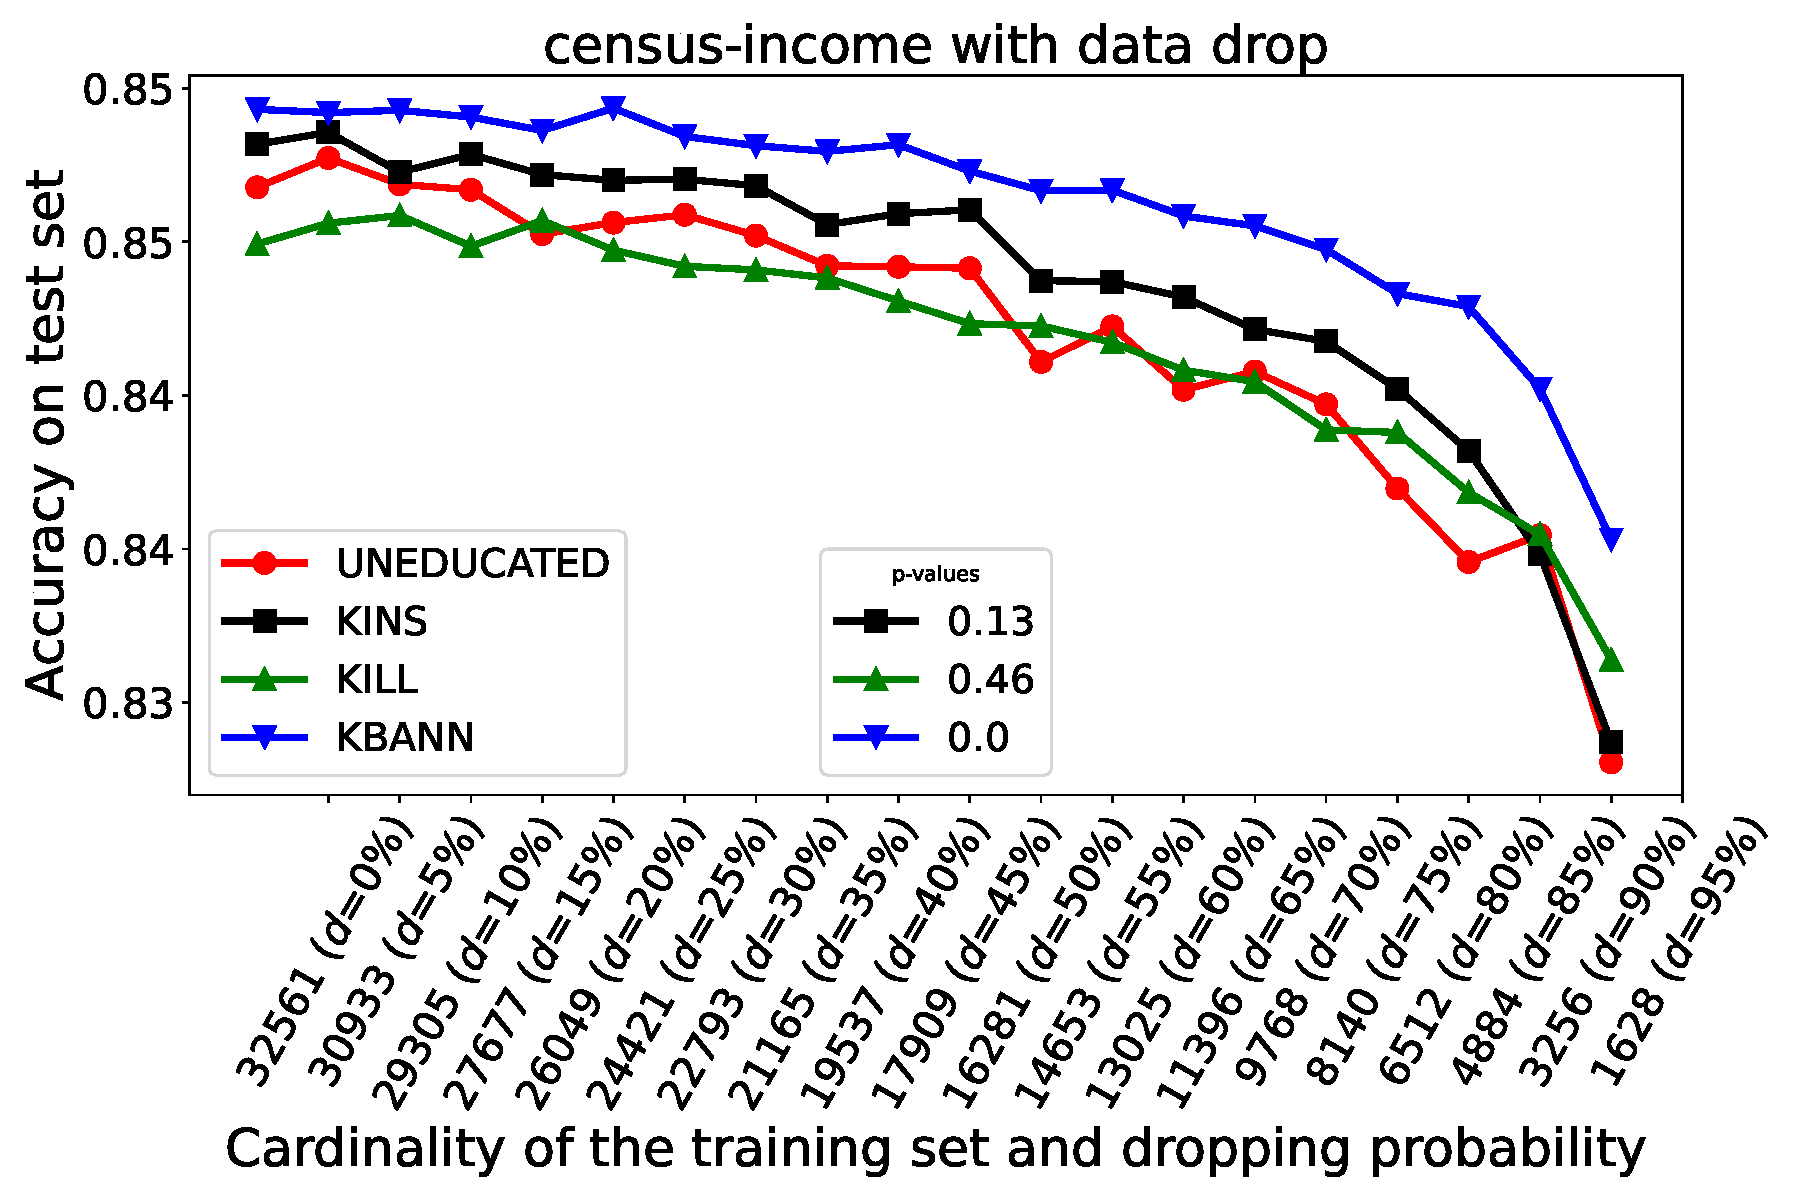
\includegraphics[width=\linewidth]{figures/drop/census-income/uneducated-kins-kill-kbann-accuracy-average-curves}
	\end{subfigure}

	\begin{subfigure}{\cellsize}
		\caption{}
		\label{fig:bcw-noise}
		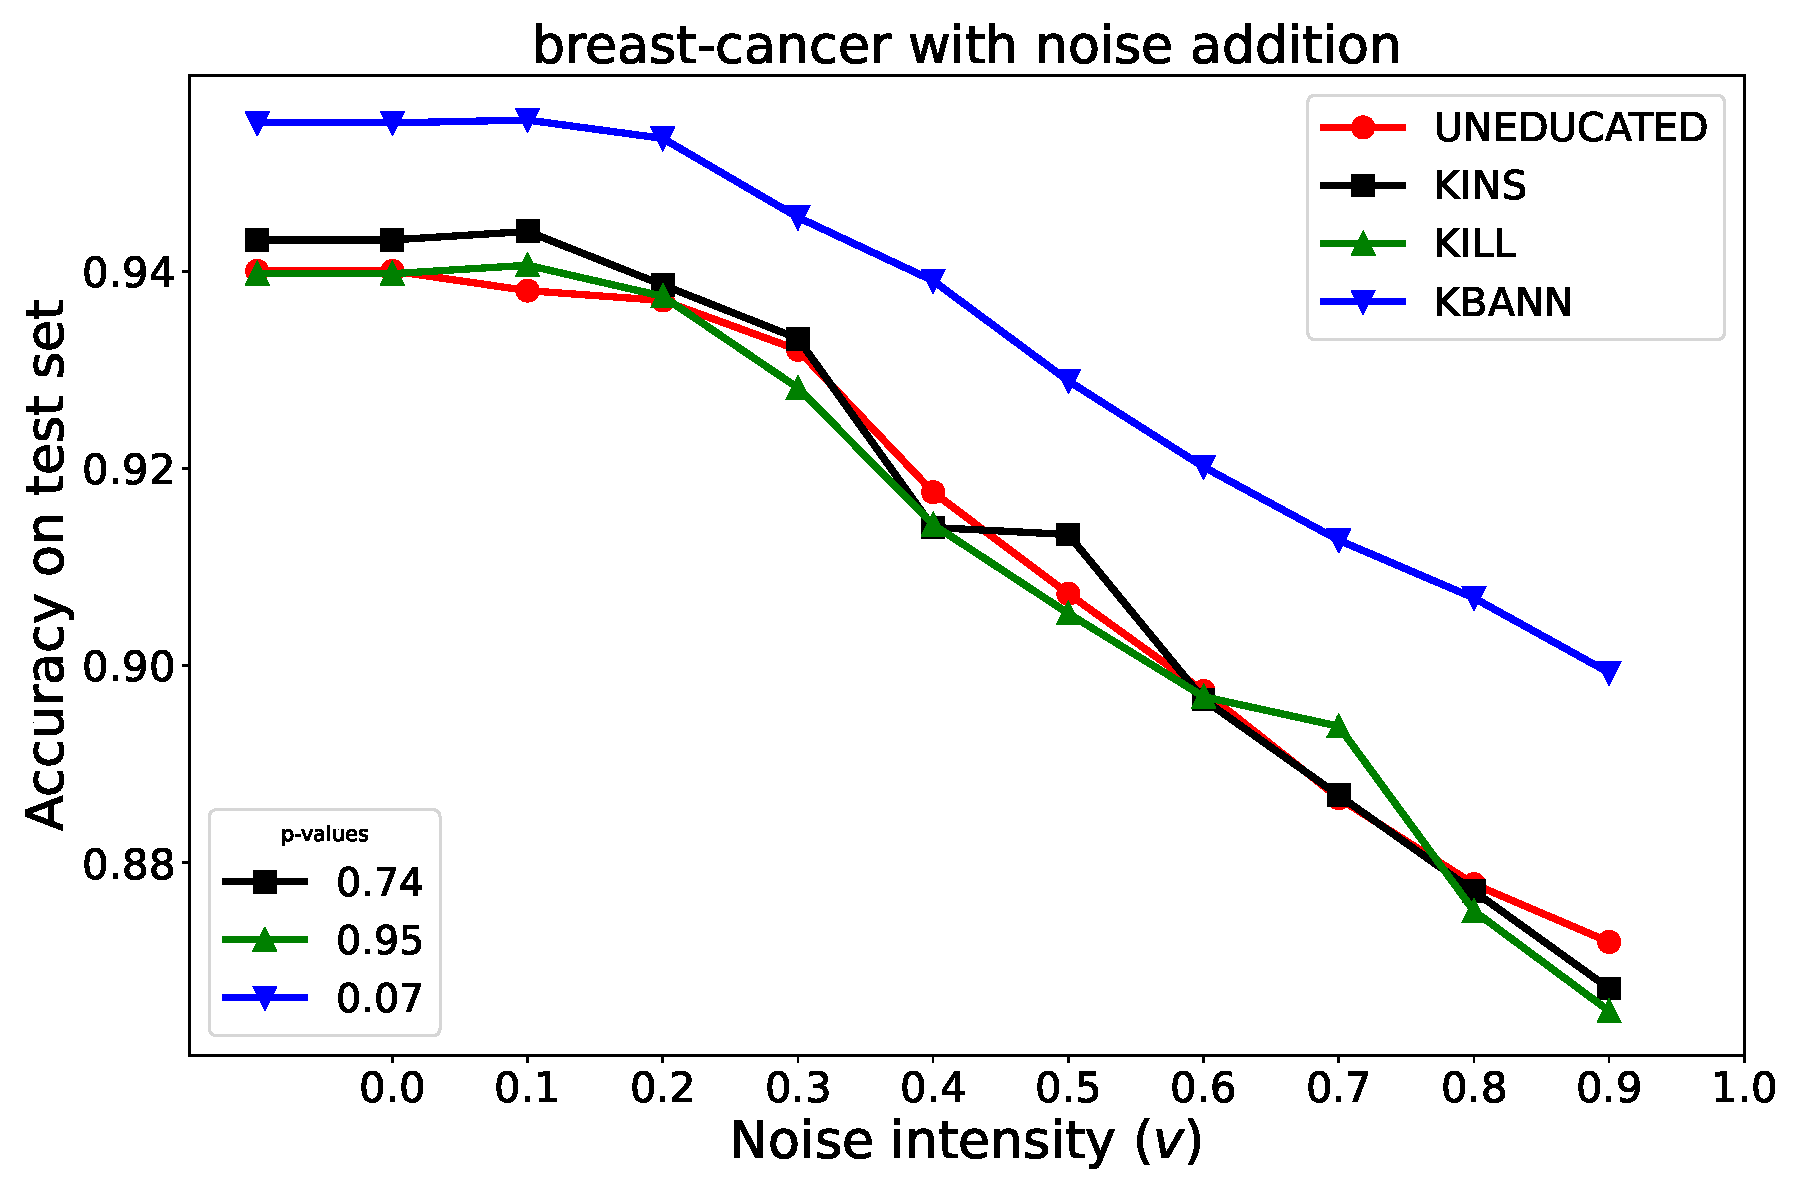
\includegraphics[width=\linewidth]{figures/noise/breast-cancer/uneducated-kins-kill-kbann-accuracy-average-curves}
	\end{subfigure}\hfil
	\begin{subfigure}{\cellsize}
		\caption{}
		\label{fig:psjgs-noise}
		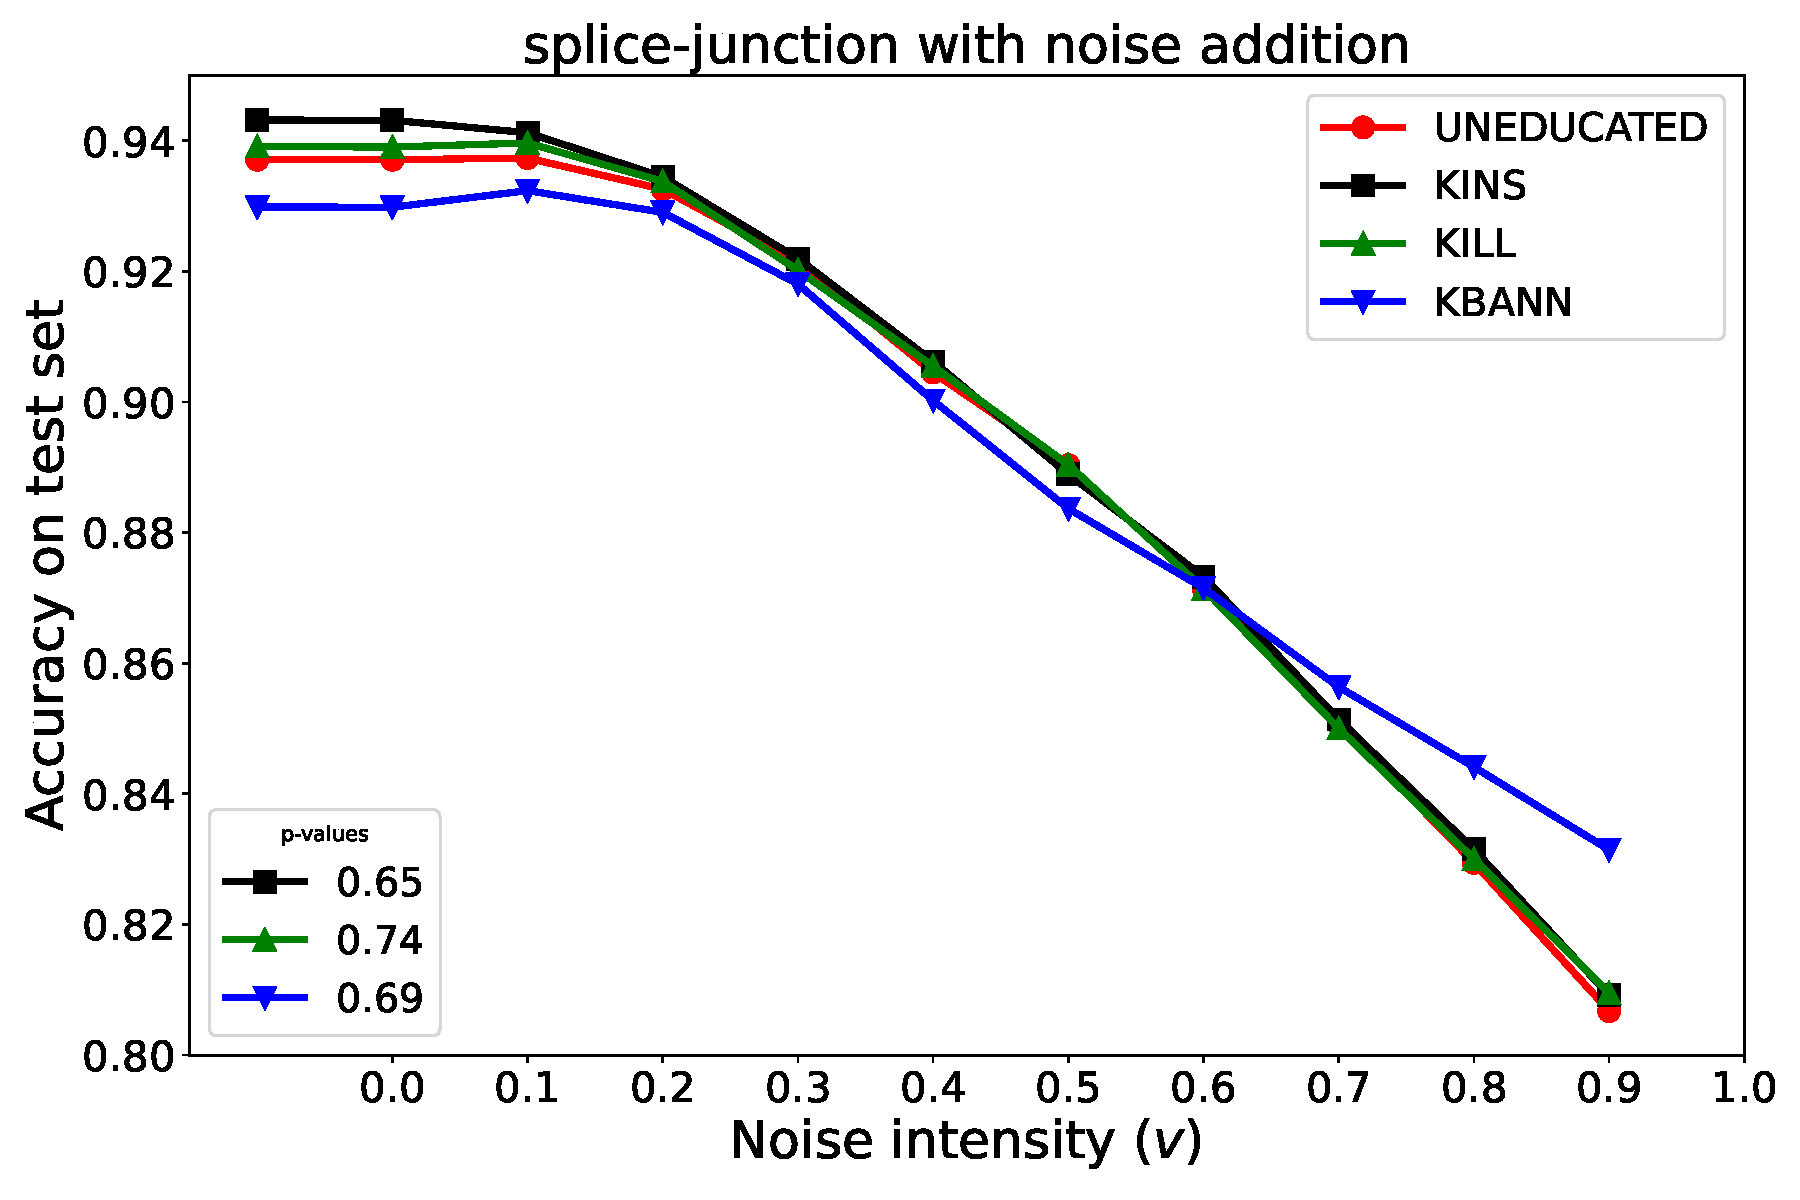
\includegraphics[width=\linewidth]{figures/noise/splice-junction/uneducated-kins-kill-kbann-accuracy-average-curves}
	\end{subfigure}\hfil
	\begin{subfigure}{\cellsize}
		\caption{}
		\label{fig:ci-noise}
		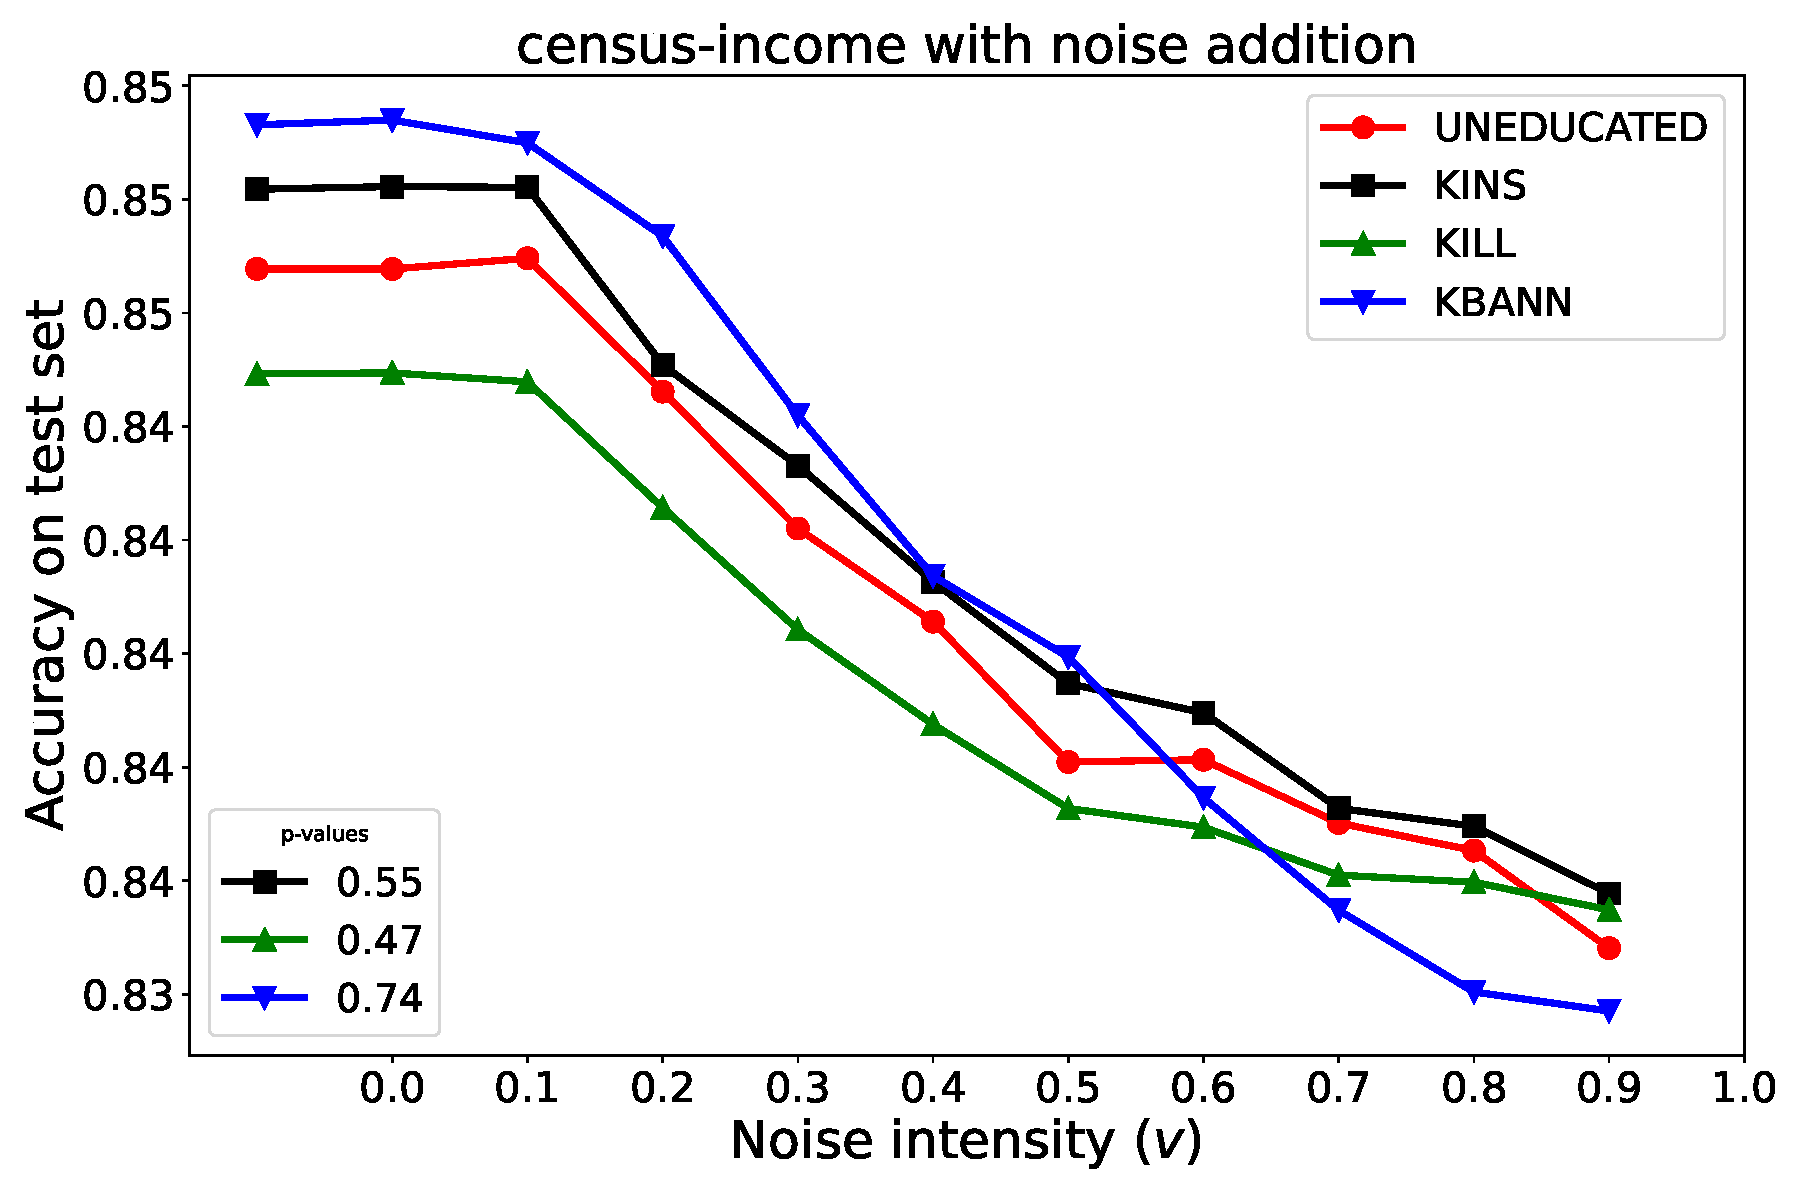
\includegraphics[width=\linewidth]{figures/noise/census-income/uneducated-kins-kill-kbann-accuracy-average-curves}
	\end{subfigure}

	\begin{subfigure}{\cellsize}
		\caption{}
		\label{fig:bcw-label}
		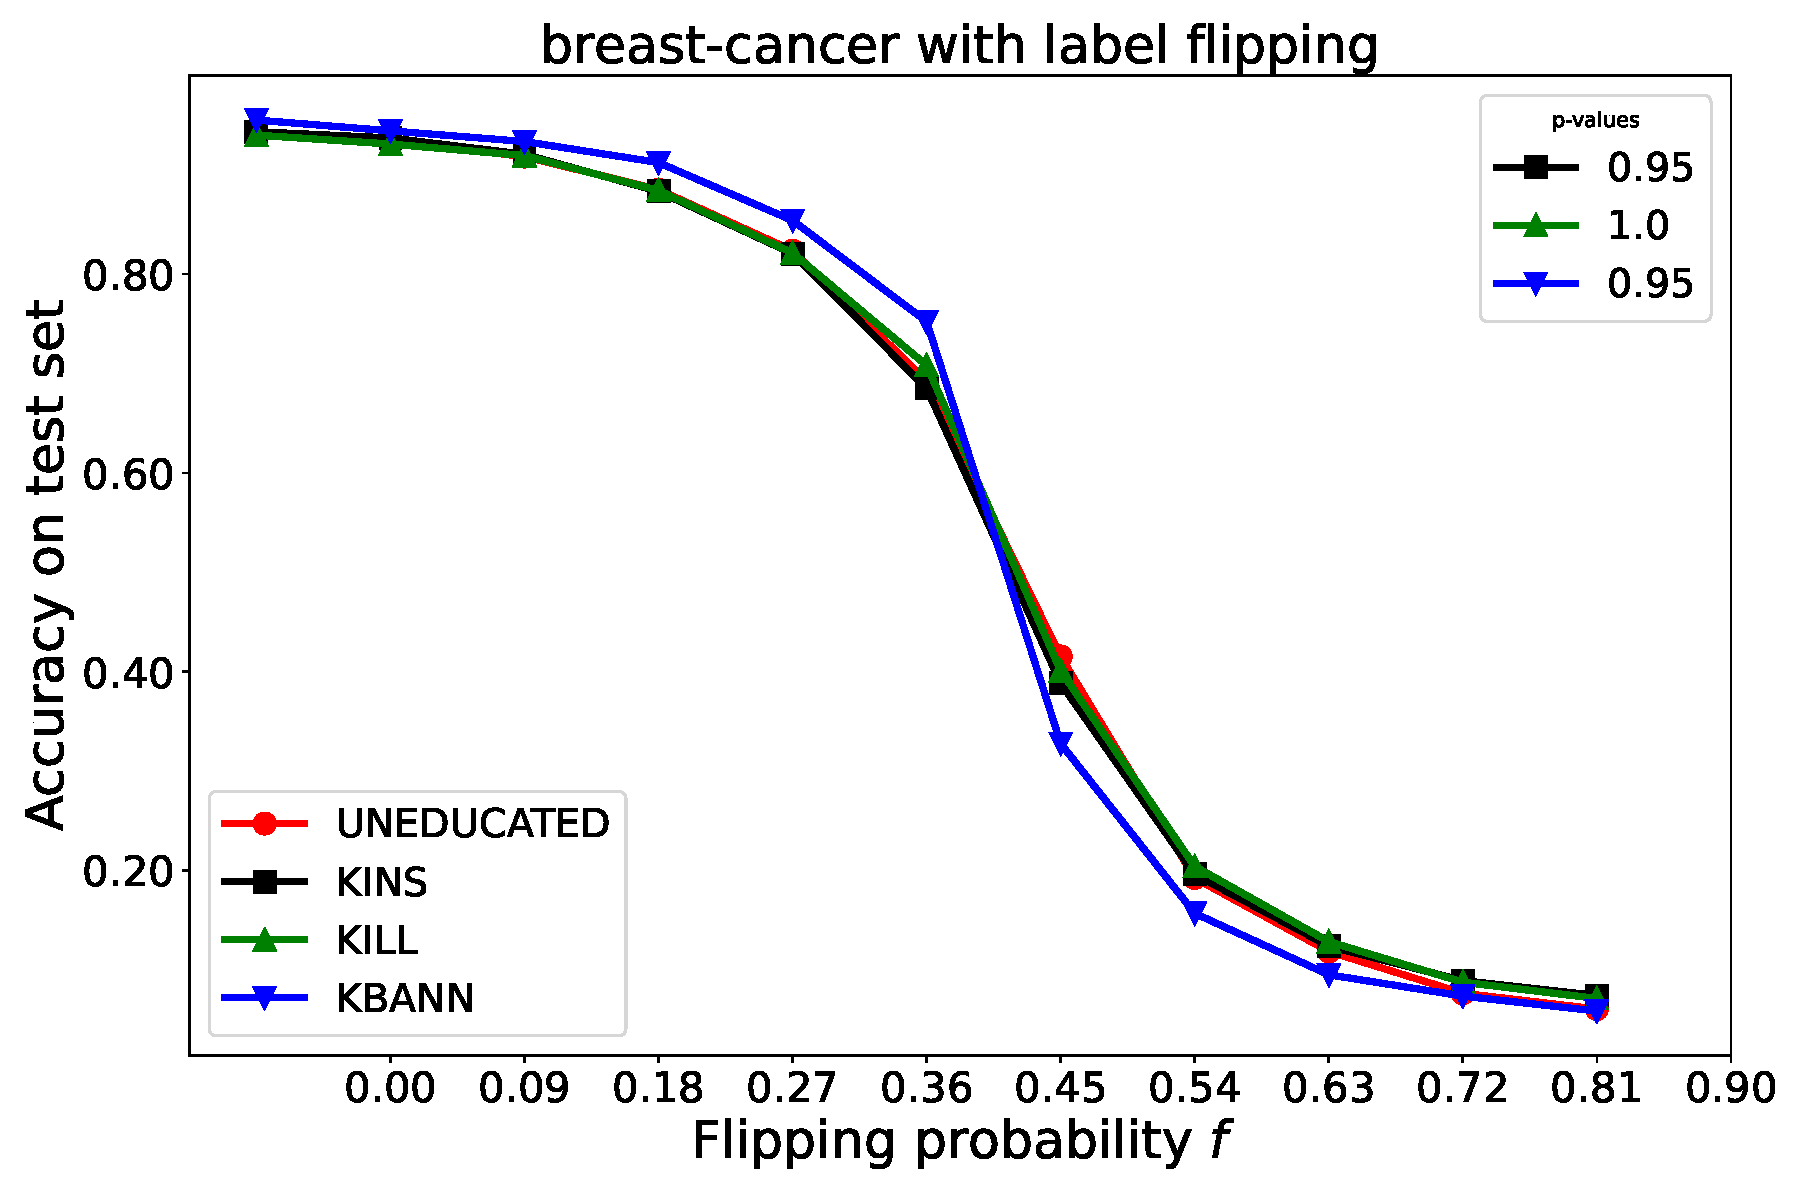
\includegraphics[width=\linewidth]{figures/label_flip/breast-cancer/uneducated-kins-kill-kbann-accuracy-average-curves}
	\end{subfigure}\hfil
	\begin{subfigure}{\cellsize}
		\caption{}
		\label{fig:psjgs-label}
		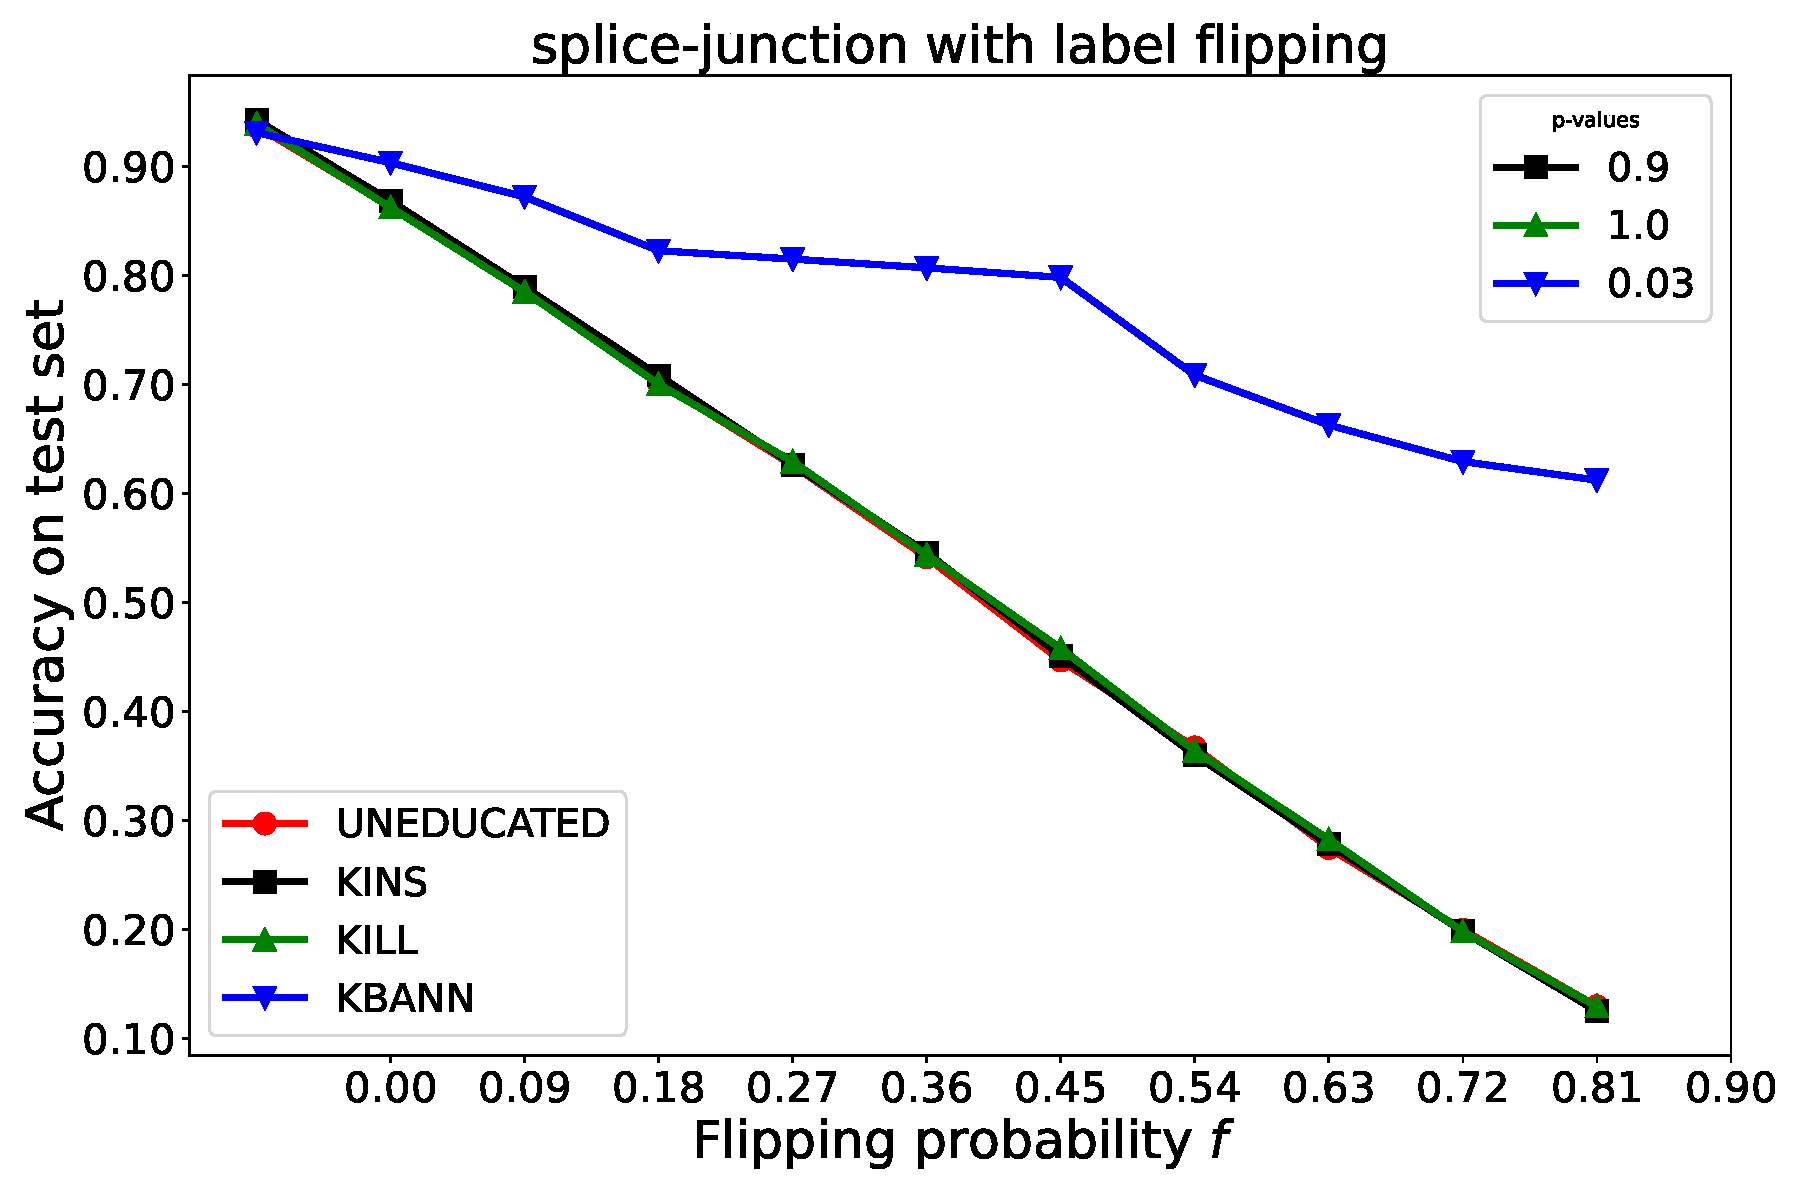
\includegraphics[width=\linewidth]{figures/label_flip/splice-junction/uneducated-kins-kill-kbann-accuracy-average-curves}
	\end{subfigure}\hfil
	\begin{subfigure}{\cellsize}
		\caption{}
		\label{fig:ci-label}
		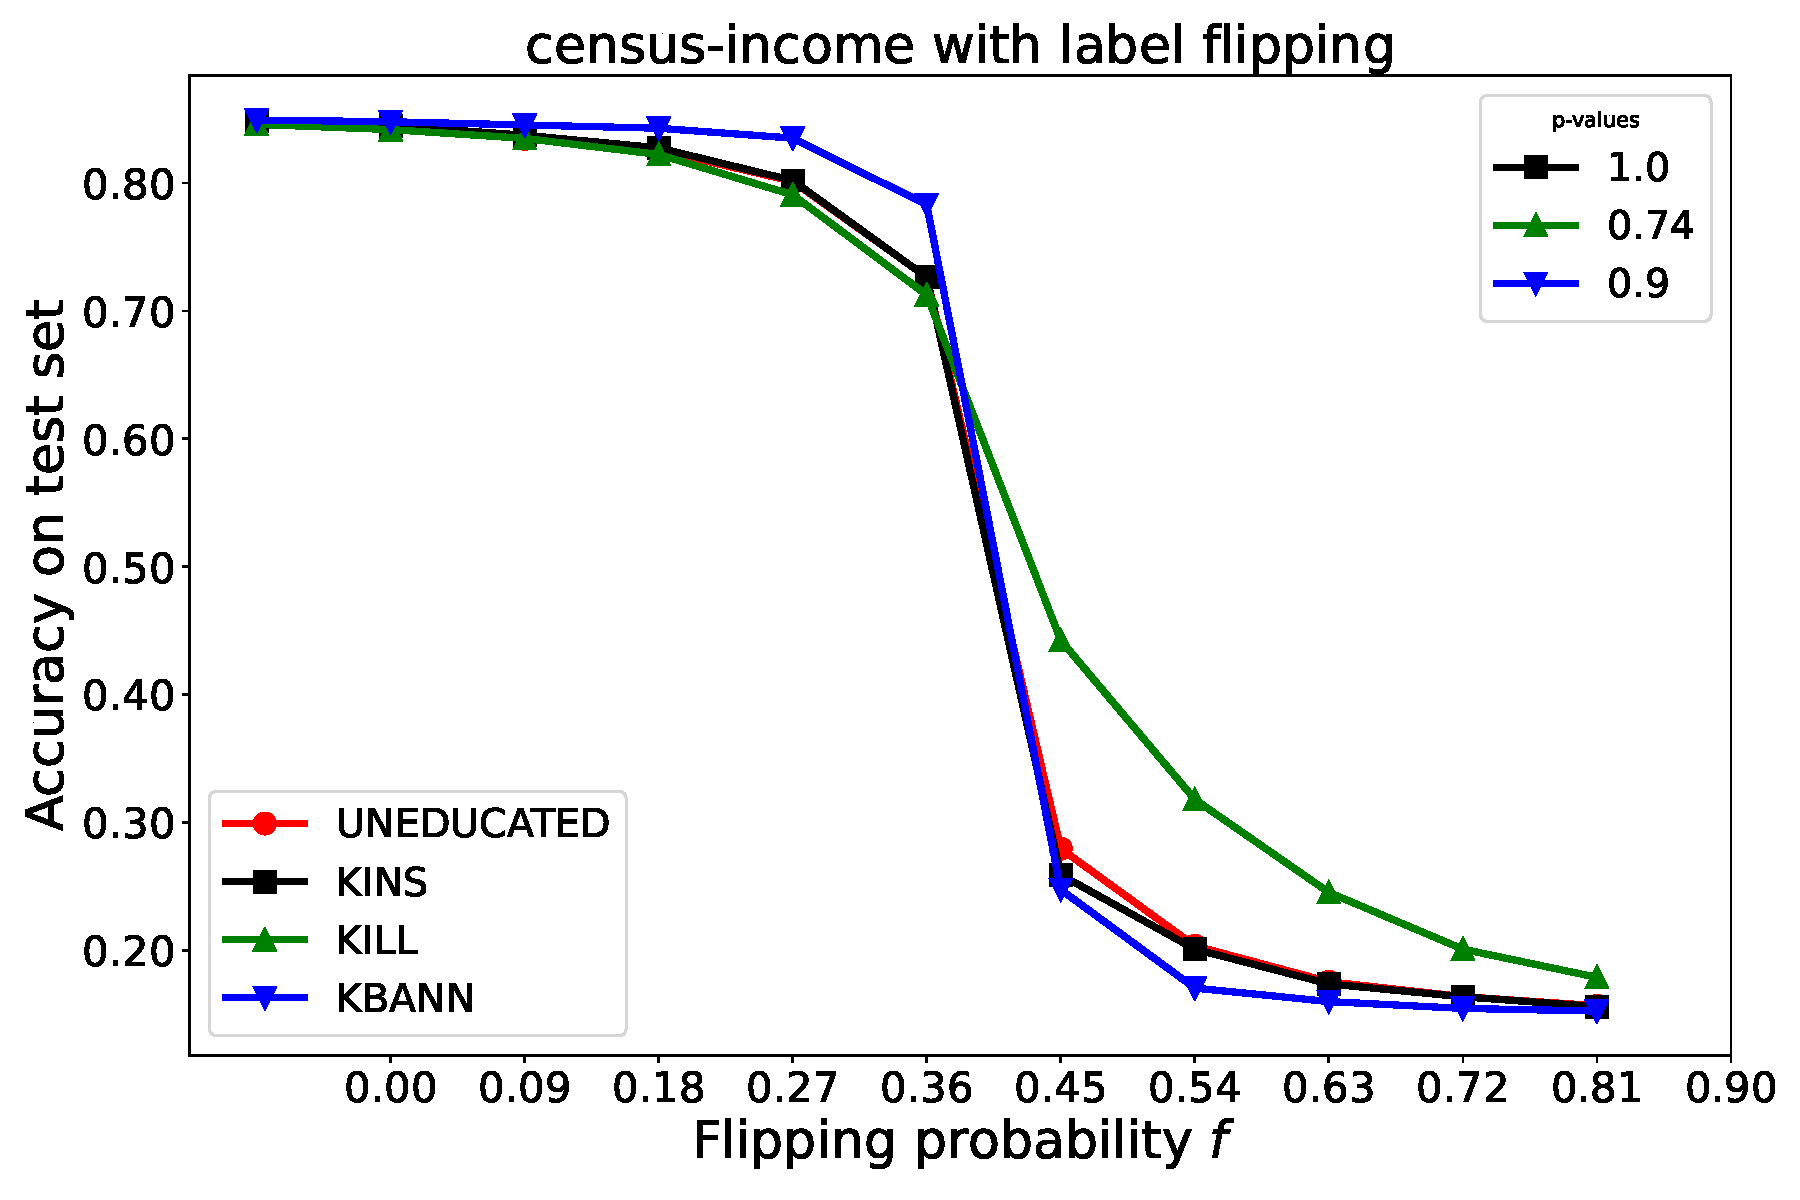
\includegraphics[width=\linewidth]{figures/label_flip/census-income/uneducated-kins-kill-kbann-accuracy-average-curves}
	\end{subfigure}
	\caption{Average accuracy over different datasets with different perturbation strategies}
	\label{fig:accuracy-results}
\end{figure*}
%
\note{TODO: generate again the figures because there is an issue with the x ticks labels}
%
% !TeX root = ../phd-thesis.tex
\begin{table}
    \centering
     \resizebox{\columnwidth}{!}{
         \begin{tabular}{l||rrr|rrr|rrr}
             \toprule
             \multirow{2}{*}{Dataset} &  \multicolumn{3}{c|}{$R_{N, D}(\mathcal{I})$ drop} &  \multicolumn{3}{c|}{$R_{N, D}(\mathcal{I})$ noise} &  \multicolumn{3}{c}{$R_{N, D}(\mathcal{I})$ flip}\\
             \cmidrule{2-10}
             & KINS &  KILL &  KBANN & KINS &  KILL &  KBANN & KINS &  KILL &  KBANN\\
             \midrule
             BCW    & \textbf{1.0493} & \textbf{1.0318} & \textbf{1.0382}  & 0.9960 & 0.9985 & \textbf{1.0109} & 0.9994 & \textbf{1.0184} & 0.9520\\
             PSJGS & \textbf{1.0045} & 0.9968 & 0.8425 & 0.9950 & 0.9984 & \textbf{1.0145} & 0.9962 &  \textbf{1.0026} & \textbf{1.6749} \\
             CI   &  0.9998 & \textbf{1.0039} & \textbf{1.0043} & 0.9992 & \textbf{1.0012} &  0.9965 & 0.9897 & \textbf{1.1703} & 0.9815 \\
             \bottomrule
         \end{tabular}
     }
    \caption[Robustness relative scores for drop, noise and label flip perturbations]{
        %
        Robustness relative scores $R_{N, D}(\mathcal{I})$ for the three perturbation strategies: drop, noise and label flip.
        %
        Bold numbers are the ones greater than 1 (i.e., the educated model is more robust than the uneducated one).
    }
    \label{tab:robustness}
\end{table}


%
This section presents the results of our experiments, focusing on the robustness of educated and uneducated predictors under different perturbation strategies.
%
To compare their performance, we use the Mann-Whitney U Test~\cite{placeholder}, a non-parametric statistical test.
%
A p-value \(\geq 0.05\) indicates no significant difference between the average accuracy distributions, while a p-value \(< 0.05\) suggests otherwise.
%
\paragraph{Data Drop}
%
In the \emph{data drop} experiments (Figure~1a-c), \gls{KBANN} is the only predictor showing significant improvements compared to the uneducated model.
%
It performs better on the \gls{BCW} (Figure~1a) and \gls{CI} (Figure~1c) datasets but exhibits a sharp decline on the \gls{PSJGS} dataset (Figure~1b) when 60\% of the data is removed (\(d = 0.6\)).
%
\gls{KINS} shows slightly better performance than the uneducated model, with a p-value of 0.01 on the \gls{BCW} dataset, indicating significant differences.
%
Overall, educated predictors improve robustness in 6 out of 9 experiments, as shown in Table~1.
%
\paragraph{Noise Addition}
%
The \emph{noise addition} experiments (Figure~1d-f) reveal that \gls{SKI} mechanisms are more sensitive to noise than to missing data.
%
Predictors trained on noisy data show a rapid decline in accuracy, starting early in the perturbation process.
%
\gls{KBANN} outperforms other methods and the uneducated model on the \gls{BCW} dataset (Figure~1d) but performs poorly on the \gls{CI} (Figure~1f) and \gls{PSJGS} (Figure~1e) datasets.
%
Interestingly, \gls{KINS} performs worse than \gls{KBANN}, likely due to its trainable modules being more prone to overfitting noisy data.
%
\gls{KILL} shows similar or worse performance compared to the uneducated model, suggesting that its penalty-based approach does not effectively handle noise perturbations.
%
\paragraph{Label Flipping}
%
In the \emph{label flipping} experiments (Figure~1g-i), predictors exhibit similar behavior on the \gls{BCW} (Figure~1g) and \gls{CI} (Figure~1i) datasets, with no significant differences (p-values close to 1).
%
Performance degrades rapidly when more than 54\% of labels are flipped (\(f = 0.54\)).
%
On the \gls{PSJGS} dataset (Figure~1h), \gls{KBANN} retains nearly 70\% accuracy even at the highest flipping probability (\(f = 0.9\)), outperforming other models, which drop to 20\%.
%
This highlights \gls{KBANN}'s strong adherence to injected knowledge, which mitigates the impact of flipped labels.
%
\gls{KILL} demonstrates good robustness across all datasets, likely due to its loss manipulation strategy, which de-emphasizes corrupted labels during training.
%
\paragraph{Discussion and Take-Home Message}
%
The experiments show that \gls{SKI} methods are most effective in handling missing data, leveraging integrated knowledge to compensate for data scarcity.
%
However, their robustness to noise perturbations is limited, with no significant improvements observed.
%
For label flipping, \gls{KILL} performs well due to its penalty-based approach, while \gls{KBANN} excels on the \gls{PSJGS} dataset due to its strong reliance on injected knowledge.
%
In summary:
%
\begin{enumerate}
    \item \gls{SKI} methods enhance robustness under data scarcity by utilizing integrated knowledge.
    %
    \item Loss-manipulating techniques like \gls{KILL} better tolerate label corruption by reducing the impact of flawed labels.
    %
    \item Structuring-based methods like \gls{KBANN} are more robust than trainable approaches like \gls{KINS}, as they preserve the integrity of injected knowledge.
\end{enumerate}
%
These findings emphasize the importance of selecting appropriate \gls{SKI} methods based on the type of perturbation and dataset characteristics.
%! Author = matteomagnini
%! Date = 05/03/25

%----------------------------------------------------------------------------------------
\chapter[Fairness through SKI]{Fairness through \gls{SKI}}
\label{ch:fairness-through-ski}
\minitoc
%----------------------------------------------------------------------------------------

\Gls{AI} has transformed various aspects of modern society.
%
With recent groundbreaking advancements, its applications are expected to grow exponentially.
%
However, the issue of fairness has become a significant concern.
%
When \gls{AI} systems are deployed without adequate safeguards, they risk perpetuating or amplifying existing social biases.
%
For example, a recruitment system trained on historical data dominated by male hires may discriminate against female applicants, reinforcing gender bias~\cite{kochling2020genderbias}.
%
To address such challenges, numerous techniques have been developed to mitigate bias in \gls{AI}.
%
Among these, regularization-based fairness techniques have gained prominence for balancing fairness and predictive performance.
%
Regularization, initially introduced to prevent overfitting, involves adding a penalty term to the loss function during training.
%
Recently, it has been extended to promote fairness by incorporating penalties derived from fairness constraints~\cite{kamishima2011fairness}.
%
These methods aim to reduce the dependence of predictions on sensitive attributes, such as gender, making them effective for bias mitigation during optimization steps like \gls{SGD} in \gls{ML} algorithms.
%

\section{Background}\label{sec:fairness-background}
%
We provide a brief but comprehensive overview of fairness in \gls{ML} to understand our contributions without delving into the extensive literature on the topic.
%
The section is organised as follows.
%
In \Cref{subsec:fairness-motivations}, we discuss the motivations for fairness in \gls{ML} and how it is related to \gls{SKI}.
%
In \Cref{subsec:fairness-metrics}, we introduce common group fairness metrics used in the literature, along with some of their limitations that motivate the development novel metrics.
%
Finally, in \Cref{sec:fauci}, we present our contributions to fairness in \gls{ML}.


\subsection{Motivations}\label{subsec:fairness-motivations}
%
\Gls{ML} models can inherit and amplify biases present in the dataset \(D\).
%
For instance, if \(D\) contains features related to gender or race, and the data is not equally distributed across these groups, biases may arise.
%
This often occurs in datasets about hiring decisions, where historical data may reflect fewer non-male or non-white candidates.
%
A supervised model \(H\), trained on such a dataset to predict a target feature \(Y\), might incorrectly learn that gender or race influences the prediction.
%
If the predictions of \(H\) are used for decision-making, such as hiring or loan approvals, the model may discriminate against certain groups.
%
In this case, the model is said to be biased, as it replicates patterns of past discrimination.

%
Fairness interventions can mitigate these biases and are applied at different stages of the \gls{ML} workflow.
%
In the literature, these methods are categorized as:
%
\begin{itemize}
    \item \textit{Pre-processing methods}, which modify the dataset \(D\) to reduce bias before training;
    %
    \item \textit{In-processing methods}, which adjust the learning algorithm \(A\) to enforce fairness during training;
    %
    \item \textit{Post-processing methods}, which modify the predictions of the model \(H\) to achieve fairness after training.
\end{itemize}

%
A critical prerequisite for fairness interventions is the ability to measure fairness.
%
Fairness metrics quantify the extent of bias in a dataset or model and evaluate the effectiveness of mitigation techniques.
%
Formally, a fairness metric is a function that takes data as input and returns a numerical score.
%
The input data can be a dataset \(D = (X, Y)\) or the predictions \(h(X)\) of a model on \(D\).
%
A lower score typically indicates higher bias, while a higher score reflects greater fairness.

%
Numerous fairness metrics have been proposed, differing in the type of data they accept and their interpretation of fairness or bias.
%
These metrics are often categorized based on the fairness notion they adhere to~\cite{mehrabi2022fairness}.
%
The two most common notions are \textit{group fairness} and \textit{individual fairness}.


\paragraph{Group fairness}\label{par:group-fairness}
%
Group fairness ensures that distinct groups of individuals, defined by sensitive attributes, are treated equally.
%
Sensitive attributes, denoted as \( S \subset X \), are features such as \emph{gender}, \emph{race}, \emph{age}, or social status, which partition the dataset \( D \) into protected groups.
%
These groups can be defined by a single sensitive attribute, e.g., the group of women identified by a specific value of the \textit{gender} feature, or by a combination of attributes, e.g., the group of Black women identified by both \textit{gender} and \textit{race}.
%
The principle of group fairness is commonly evaluated by measuring the correlation between sensitive attributes \( S \) and the target variable \( Y \).
%
For instance, if \( Y \) represents loan approval outcomes and \( S \) represents the applicant's race, group fairness metrics assess whether the approval rates are consistent across racial groups~\cite{placeholder}.
%
Such metrics are crucial for identifying and addressing biases in decision-making processes.


\paragraph{Individual fairness}\label{par:individual-fairness}
%
Individual fairness ensures that similar individuals receive similar treatment.
%
The simplest approach to individual fairness is \emph{fairness through awareness}.
%
This method relies on a distance metric \(\delta : X \times X \to \mathbb{R}\) in the input space (e.g., Euclidean distance).
%
It requires that if two individuals \(x_1\) and \(x_2\) are similar up to a threshold \(\epsilon\), i.e., \(\delta(x_1, x_2) < \epsilon\), then their corresponding target values \(y_1\) and \(y_2\) should also be similar.
%
In practice, model predictions \(h(x_1)\) and \(h(x_2)\) are compared instead of true labels, and fairness scores are computed by averaging the differences in predictions for similar instances.
%
Another approach is \emph{fairness through unawareness}, which requires that sensitive attributes are not used by the model during training or prediction.
%
This can be achieved by removing sensitive features from the dataset or ensuring the model does not rely on them.
%
Fairness scores in this case measure the extent to which the model depends on sensitive attributes and penalize such reliance.
%
A more advanced formulation is \emph{counterfactual fairness}.
%
This requires that a model's prediction for an individual \(x\) remains the same, regardless of whether \(x\) belongs to a group \(s\) in the actual dataset or to a counterfactual group \(s' \neq s\).
%
Counterfactual fairness ensures that predictions are invariant to changes in sensitive attributes across hypothetical scenarios.
%
As individual fairness is not the primary focus of this work, we do not delve into the specific metrics used to evaluate it.
%
For a detailed discussion, the reader is referred to~\cite{mehrabi2022fairness}.


\paragraph{Fairness and SKI}\label{par:fairness-ski}
%
How promoting fairness in \gls{ML} models can be achieved through \gls{SKI} methods?
%
It is definitively possible if we keep our attention on \emph{in-processing} methods, which enforce fairness during model training, and on \emph{group fairness} metrics, which measure the extent to which a model is biased against certain groups.
%
Indeed, the process of including fairness constraints in the training loss can be seen as a form of regularization, similar to how \gls{SKI} methods incorporate constraints into the optimization process.
%
The knowledge that usually \gls{SKI} methods leverage is about the \gls{ML} task at hand (e.g., classification, regression) and the relationships between features and target variables, most commonly in order to improve generalization and interpretability.
%
In the context of fairness, this knowledge includes fairness-related constraints -- still consisting in relationships between features and target variables -- that are used to ensure that the model does not discriminate against certain groups based on \emph{sensitive attributes}.
%
Instead of using logical operators between expressions involving features and constants (see for example \Cref{subsec:kill-validation}), fairness metrics are directly involved.
%
Still, a knowledge of this kind can be expressed with a symbolic formalism, and therefore the whole process can be seen as a form of \gls{SKI} according \Cref{def:ski}.


\subsection{Fairness metrics}\label{subsec:fairness-metrics}
%
We introduce three of the most popular \emph{group fairness} metrics used in \gls{ML} to evaluate the fairness of models.
%
Despite being used in many works, these metrics suffer certain limitations, such as being applicable only to binary classification tasks or requiring specific types of sensitive attributes.
%
In particular, all three metrics -- as defined below in their first formulation -- can support only binary or categorical sensitive attributes, i.e., \( A \in \{0, 1\} \) or \( A \in \{a_1, a_2, \ldots, a_n\} \) for some \( n \in \mathbb{N} \).
%
Moreover, the metrics do not take into account the option to weight groups differently.
%
This possibility could be useful in scenarios of highly unbalanced groups.
%
These limitations are the driver that will lead to the development of novel fairness metrics in \Cref{sec:fauci}.


\Glsfull{DP} is a fairness metric, also referred to as \emph{statistical parity}, that evaluates whether the predictions of a \gls{ML} model are independent of a given protected attribute.
%
This implies that the values of the sensitive feature do not influence the model's output~\cite{placeholder}.
%
\Gls{DP} compares the distribution of the model's predictions with the distribution of predictions conditioned on the values of the sensitive attribute.
%
For a binary classifier \( h \) and a discrete sensitive attribute \( A \), \gls{DP} is mathematically defined as:
%
\begin{equation}
    \label{eq:dp}
    \text{DP}_{h,A}(X) = \sum_{a \in A} \left| \mathbb{E}[h(X) \mid A = a] - \mathbb{E}[h(X)] \right|,
\end{equation}
%
where \( X \) represents the test data, \( A \) denotes the sensitive attribute, \( a \) is a specific value of \( A \), \( \mathbb{E} \) is the expectation operator, and \( \left| \cdot \right| \) is the absolute value.
%
A model \( h \) satisfies DP if the computed value is below a predefined bias threshold \( \epsilon \), commonly set to \( 0.01 \).
%
\Gls{DP} is particularly useful in applications such as loan approvals, where it ensures that approval rates are consistent across demographic groups, thereby mitigating discrimination.


\Glsfull{DI} quantifies the disproportionate effect of a classifier on individuals based on a sensitive attribute~\cite{placeholder}.
%
For binary classification tasks and binary sensitive attributes, \gls{DI} is initially defined as the ratio:
%
\begin{equation}
    \label{eq:di_unbounded}
    \text{di}_{h,A}(X) = \frac{\mathbb{E}[h(X) \mid A = 1]}{\mathbb{E}[h(X) \mid A = 0]}.
\end{equation}
%
To ensure bounded values within \([0, 1]\), DI is commonly standardized using the function \( \eta(x) = \min\{x, x^{-1}\} \), resulting in:
%
\begin{equation}
    \label{eq:di}
    \text{DI}_{h,A}(X) = \eta(\text{di}_{h,A}(X)).
\end{equation}
%
Values of \gls{DI} above \( 0.8 \) are generally considered acceptable, with lower values indicating higher fairness violations.
%
In scenarios requiring positive scores, \( 1 - \text{DI} \) may be reported, such as during the training of neural networks.
%
\Gls{DI} is applicable in contexts like loan approvals, where it helps identify disproportionate denial rates affecting specific demographic groups.


\Glsfull{EO} measures the extent to which a classifier predicts a given class equally across all values of a sensitive attribute~\cite{placeholder}.
%
For binary classification (\( Y \in \{0, 1\} \)) and a categorical sensitive attribute \( A \), \gls{EO} is defined as:
%
\begin{equation}
    \label{eq:eo}
    \text{EO}_{h,A}(X) = \sum_{(a, y) \in A \times Y} \text{eo}_{h,A}(X, a, y),
\end{equation}
%
where \( Y \) represents the ground truth, and \( \text{eo}_{h,A}(X, a, y) \) is given by:
%
\begin{equation}
    \label{eq:eo_partial}
    \text{eo}_{h,A}(X, a, y) = \left| \mathbb{E}[h(X) \mid A = a, Y = y] - \mathbb{E}[h(X) \mid Y = y] \right|.
\end{equation}
%
Similar to \gls{DP}, a classifier is considered fair if its \gls{EO} value is below a predefined bias threshold \( \epsilon \).
%
\Gls{EO} is valuable in applications like loan approvals, where it identifies disparities in approval rates that may favor specific demographic groups.




\section[Fairness under constraints injection]{\Glsentrylong{FaUCI}}\label{sec:fauci}
%
In this section, we present the contribution of the work ``Enforcing Fairness via Constraint Injection with FaUCI''~\cite{DBLP:conf/aequitas/MagniniCCO24}, presented at the 2nd AEQUITAS workshop on fairness and bias in \gls{AI} 2024.
%
The work introduces two distinct contributions: the introduction of novel fairness metrics -- more precisely the extensions of \gls{DP}, \gls{DI}, and \gls{EO} to categorical and continuous sensitive attributes -- and the development of a novel fairness regularization method, called \gls{FaUCI}, which injects fairness constraints into the training loss of a model.


\subsection{Novel fairness metrics}\label{subsec:novel-fairness-metrics}
%
This section introduces weighted and generalized variants of fairness metrics to support both categorical and continuous sensitive attributes.
%
These extensions aim to generalize fairness metrics beyond binary data, enabling their application to real-world datasets.
%
For instance, they allow prioritizing fairness for underrepresented groups, such as specific ethnicities, when more than two groups exist~\cite{placeholder}.
%
We focus on three metrics: \gls{DP}, \gls{DI}, and \gls{EO}, and propose their weighted and generalized formulations.


\paragraph{Weighted and Generalized Demographic Parity}
%
\Gls{DP} evaluates whether the predictions of a model are independent of a sensitive attribute.
%
For binary classification, the values \( \mathbb{E}[h(X) \mid A = a] \) and \( \mathbb{E}[h(X)] \) from \Cref{eq:dp} are bounded within \([0, 1]\).
%
The maximum theoretical value of \gls{DP} depends on the number of possible values of the sensitive attribute \( A \), i.e., \( 0 \leq \text{DP} \leq |A| \).
%
This variability makes comparisons across datasets challenging.
%
To address this, we propose two variants: \glsfull{WDP} and \glsfull{GDP}.


\Gls{WDP} is defined as:
%
\begin{equation}
    \label{eq:wdp}
    \text{WDP}_{h,A}(X) = \sum_{a \in A} \left| \mathbb{E}[h(X) \mid A = a] - \mathbb{E}[h(X)] \right| \cdot w_a,
\end{equation}
%
where \( w_a \) represents the weight of the \( a \)-th value of \( A \), and \( \sum_{a \in A} w_a = 1 \).
%
Weights can be chosen based on the distribution of \( A \) or set equally to avoid bias towards frequent values.


\Gls{GDP} extends \gls{DP} to continuous sensitive attributes:
%
\begin{equation}
    \label{eq:gdp}
    \text{GDP}_{h,A}(X) = \int_{l}^{u} \left| \mathbb{E}[h(X) \mid A = a] - \mathbb{E}[h(X)] \right| \cdot w_a \, da,
\end{equation}
%
where \( l \) and \( u \) are the minimum and maximum values of \( A \), and \( w_a \) is a user-defined weight function satisfying \( \int_{l}^{u} w_a \, da = 1 \).



\paragraph{Weighted and Generalized Disparate Impact}
%
\Gls{DI} quantifies the disproportionate effect of a classifier on groups defined by a sensitive attribute.
%
For categorical attributes, we define \glsfull{WDI} as:
%
\begin{equation}
    \label{eq:wdi}
    \text{WDI}_{h,A}(X) = \sum_{a \in A} \eta \left( \frac{\mathbb{E}[h(X) \mid A = a]}{\mathbb{E}[h(X) \mid A \neq a]} \right) \cdot w_a,
\end{equation}
%
where \( \eta(x) = \min\{x, x^{-1}\} \) ensures bounded values within \([0, 1]\).


For continuous attributes, \glsfull{GDI} is defined as:
%
\begin{equation}
    \label{eq:gdi}
    \text{GDI}_{h,A}(X) = \int_{l}^{u} \eta \left( \frac{\mathbb{E}[h(X) \mid A = a]}{\mathbb{E}[h(X) \mid A \neq a]} \right) \cdot w_a \, da.
\end{equation}


\paragraph{Weighted and Generalized Equalized Odds}
%
\Gls{EO} measures whether a classifier predicts equally across sensitive attribute values and ground truth classes.
%
To address the lack of bounded values, we define \glsfull{WEO} as:
%
\begin{equation}
    \label{eq:weo}
    \text{WEO}_{h,A}(X) = \sum_{(a, y) \in A \times Y} \text{eo}_{h,A}(X, a, y) \cdot w_a,
\end{equation}
%
where \( \text{eo}_{h,A}(X, a, y) \) is defined in \Cref{eq:eo}.


\Glsfull{GEO} extends \gls{EO} to continuous attributes:
%
\begin{equation}
    \label{eq:geo}
    \text{GEO}_{h,A}(X) = \int_{l}^{u} \left( \text{eo}_{h,A}(X, a, 0) + \text{eo}_{h,A}(X, a, 1) \right) \cdot w_a \, da.
\end{equation}
%
These weighted and generalized metrics provide a more flexible framework for evaluating fairness in diverse datasets~\cite{placeholder}.



\subsection{Novel SKI fairness method}\label{subsec:novel-fairness-method}
%
The proposed method, \gls{FaUCI}, is designed for \gls{ML} models trained using \gls{SGD}, particularly \glspl{NN}.
%
It introduces a fairness-specific cost factor into the loss function, which depends on the fairness metric to be minimized.
%
The metrics considered include \gls{WDP}, \gls{GDP}, \gls{WDI}, \gls{GDI}, \gls{WEO}, and \gls{GEO}, as defined in \Cref{subsec:novel-fairness-metrics}.
%
Unlike other methods, \gls{FaUCI} ensures that the fairness metric is bounded within \([0, 1]\), supports binary, categorical, and continuous sensitive attributes, and can address intersectional fairness.

%
The loss function is originally formulated as:
%
\begin{equation}
    \label{eq:fauci_loss}
    \mathcal{L}_{h,A}(X, Y) = E(h(X), Y) + \lambda F_{h,A}(X, Y),
\end{equation}
%
where \(E\) represents the error function, \(F_{h,A}\) is the fairness regularization term, and \(\lambda \in \mathbb{R}_{>0}\) is a hyperparameter controlling the weight of the fairness term.
%
The choice of \(E\) depends on the task, such as accuracy or cross-entropy for classification, while \(F\) is selected from the fairness metrics introduced earlier.
%
In a later work -- currently under peer review -- \Cref{eq:fauci_loss} has been modified as follows:
%
\begin{equation}
    \label{eq:fauci_loss_new}
    \mathcal{L}_{h,A}(X, Y) = (1 - \lambda) E(h(X), Y) + \lambda F_{h,A}(X, Y),
\end{equation}
%
with $0 \le \lambda \le 1$.
%
In this way the comparison between \gls{FaUCI} and other fairness methods is simplified since the range of the hyperparameter \(\lambda\) is well-defined.

%
The fairness metric \(F_{h,A}\) is computed on the input data \(X\), which is divided into batches during training.
%
The batch size, a hyperparameter of \gls{SGD}, affects the accuracy of fairness estimation.
%
Larger batch sizes improve fairness estimation but slow down the training process, creating a trade-off.

%
\gls{FaUCI} offers several advantages over existing methods.
%
First, it supports sensitive attributes of any type and is agnostic to the choice of fairness metric, making it applicable to diverse scenarios.
%
Second, it avoids the need for additional hyperparameter tuning, such as those required by \gls{KDE}-based methods~\cite{placeholder}.
%
Third, the weighted fairness metrics introduced in \Cref{subsec:novel-fairness-metrics} mitigate biases in unbalanced datasets, ensuring fairness across underrepresented groups.
%
Finally, \gls{FaUCI} is extensible to other fairness metrics and can be adapted for intersectional fairness, as discussed in \Cref{subsubsec:intersectional-fairness}.



\subsubsection{Theoretical Analysis}
\label{subsubsec:theoretical}
%
During the training of a \gls{NN}, the training set is divided into batches.
%
For each epoch, all batches are processed once for inference (forward propagation) and gradient descent (backpropagation).
%
Between these steps, the loss function is computed to update the model parameters.
%
This section outlines algorithms for computing the fairness cost factor for \gls{WDP}, \gls{WDI}, and \gls{WEO} metrics.
%
Continuous variants are omitted as their computation follows identical steps.
%
For simplicity, the weights are chosen based on the frequencies of the sensitive attribute values, which does not affect the computational complexity.

\begin{algorithm}
    \caption{Weighted Demographic Parity (returns $wdp$)}
    \label{alg:wdp}
    \begin{algorithmic}[1]
        \REQUIRE $h$ \hfill predictive model
        \REQUIRE $A$ \hfill sensitive attribute
        \REQUIRE $batch$ \hfill dataset batch
        \STATE $wdp \leftarrow 0$
        \STATE $estimated \leftarrow \mathbb{E}[h(batch)]$
        \FORALL{$a$ in $A$}
            \STATE $estimated\_a \leftarrow \mathbb{E}[h(batch) \mid A = a]$
            \STATE $p\_a \leftarrow \mathbb{P}[A = a]$
            \STATE $wdp \leftarrow wdp + \left( \| estimated - estimated\_a \| \cdot p\_a \right)$
        \ENDFOR
    \end{algorithmic}
\end{algorithm}

%
\Cref{alg:wdp} computes the \gls{WDP} metric for a single batch.
%
The cost of estimating probabilities in line 2 is \(O(B)\), where \(B\) is the batch size.
%
Lines 4 and 5 also have a cost of \(O(B)\), while line 6 has a constant cost.
%
These steps are repeated for each value of \(A\), resulting in a total computational cost of \(O(B) + 2O(BN) + O(N) = O(BN)\), where \(N\) is the number of distinct values of \(A\).

\begin{algorithm}
    \caption{Weighted Disparate Impact (returns $wdi$)}
    \label{alg:wdi}
    \begin{algorithmic}[1]
        \REQUIRE $h$, $A$, $batch$ \hfill as in \Cref{alg:wdp}
        \STATE $wdi \leftarrow 0$
        \FORALL{$a$ in $A$}
            \STATE $est\_a \leftarrow \mathbb{E}[h(batch) \mid A = a]$
            \STATE $est\_not\_a \leftarrow \mathbb{E}[h(batch) \mid A \neq a]$
            \STATE $p\_a \leftarrow \mathbb{P}[A = a]$
            \STATE $wdi \leftarrow wdi + \left( \min\left\{ \frac{est\_a}{est\_not\_a}, \frac{est\_not\_a}{est\_a} \right\} \cdot p\_a \right)$
        \ENDFOR
    \end{algorithmic}
\end{algorithm}

%
\Cref{alg:wdi} computes the \gls{WDI} metric.
%
Lines 3, 4, and 5 have a cost of \(O(B)\), while line 6 has a constant cost.
%
These steps are repeated \(N\) times, resulting in a total computational cost of \(3O(BN) + O(N) = O(BN)\).

\begin{algorithm}
    \caption{Weighted Equalized Odds (returns $weo$)}
    \label{alg:weo}
    \begin{algorithmic}[1]
        \REQUIRE $h$, $A$, $batch$ \hfill as in \Cref{alg:wdp}, \hfill $Y$: ground truth
        \STATE $weo \leftarrow 0$
        \STATE $est\_y\_i \leftarrow \mathbb{E}[h(batch) \mid Y = i]$ \hfill \(\forall i \in \{0, 1\}\)
        \FORALL{$a$ in $A$}
            \STATE $est\_a\_y\_i \leftarrow \mathbb{E}[h(batch) \mid A = a, Y = i]$ \hfill \(\forall i \in \{0, 1\}\)
            \STATE $p\_a \leftarrow \mathbb{P}[A = a]$
            \STATE $weo\_i \leftarrow \| est\_a\_y\_i - est\_y\_i \|$ \hfill \(\forall i \in \{0, 1\}\)
            \STATE $weo \leftarrow weo + \left( (weo\_0 + weo\_1) \cdot p\_a \right)$
        \ENDFOR
    \end{algorithmic}
\end{algorithm}

%
\Cref{alg:weo} computes the \gls{WEO} metric for binary classification tasks.
%
Lines 2 and 3 have a cost of \(O(B)\), while lines 5-7 inside the loop also cost \(O(B)\).
%
Lines 8-10 have a constant cost.
%
The total computational cost is \(2O(B) + 3O(BN) + 3O(N) = O(BN)\).

%
All three algorithms have a computational cost linear in both the batch size (\(B\)) and the number of values of \(A\) (\(N\)).
%
For continuous sensitive attributes, the computation involves integrals instead of discrete values.
%
The implementation used in experiments relies on histogram-based methods, dividing the range of \(A\) into non-overlapping intervals of equal width.
%
In this case, the computational cost depends on the number of intervals rather than the number of distinct values of \(A\).



\subsubsection{Intersectional fairness extension}\label{subsubsec:intersectional-fairness}
%
\Gls{FaUCI} is extended to optimize fairness in intersectional settings, where subgroups formed by the intersections of protected attributes are considered.
%
This extension supports fairness metrics involving multiple sensitive attributes through two approaches.
%
The first approach creates a dummy protected attribute by combining the original attributes, enabling \gls{FaUCI} to optimize fairness for the intersection of these attributes.
%
However, this method may become computationally intractable due to the increased complexity of the fairness metric~\cite{placeholder}.
%
To address this, an alternative approach is proposed.
%
The second approach combines multiple loss factors, each penalizing fairness violations for a single protected attribute.
%
The modified loss function is defined as:
%
\begin{equation}
    \label{eq:intersectional_loss}
    \mathcal{L}_{h,\bar{A}}(X, Y) = E(h(X), Y) + \lambda_1 F_{h,A_1}(X) + \cdots + \lambda_n F_{h,A_n}(X),
\end{equation}
%
where \(\bar{A}\) represents a set of protected attributes \(\{A_1, \ldots, A_n\}\), \(E\) is the error function, and \(F_{h,A_i}\) is the fairness regularization term for attribute \(A_i\).
%
This formulation ensures that the computational cost of the fairness metric remains linear in the number of attributes, rather than exponential.
%
It provides a trade-off between computational efficiency and the complexity of the fairness metric.
%
Further details and empirical results on \gls{FaUCI} in intersectional fairness contexts will be presented in future work~\cite{placeholder}.

\printbibliography[title=References,heading=bibintoc]
\end{refsection}

%----------------------------------------------------------------------------------------
%------------------------------------- PART III -----------------------------------------
%----------------------------------------------------------------------------------------

\part{Engineering of intelligent systems}\label{part:engineering-of-intelligent-systems}

\begin{refsection}
%! Author = matteomagnini
%! Date = 05/03/25

%----------------------------------------------------------------------------------------
\chapter{NeSy AI for real world applications}
\label{ch:nesy-ai-for-real-world-applications}
\minitoc
%----------------------------------------------------------------------------------------

\section{Motivations}\label{sec:nesy-ai-motivations}

\section{Goals and challenges}\label{sec:nesy-ai-goals-and-challenges}

\section{Applications}\label{sec:nesy-ai-applications}

\subsection{\Gls{SKE} for explainable nutritional recommenders}\label{subsec:ske-for-explainable-nutritional-recommenders}

\subsection{A general-purpose protocol for multi-agent based explanations}\label{subsec:a-general-purpose-protocol-for-multi-agent-based-explanations}

\subsection{\Glsentrylong{NeSy} \Gls{AI} for supporting chronic disease diagnosis and monitoring}\label{subsec:nesy-ai-for-supporting-chronic-disease-diagnosis-and-monitoring}

\subsection{\Gls{LLM}-based solutions for healthcare chatbots: a comparative analysis}\label{subsec:llm-based-solutions-for-healthcare-chatbots-a-comparative-analysis}

\subsection{Open-source small language models for personal medical assistant chatbots}\label{subsec:open-source-small-language-models-for-personal-medical-assistant-chatbots}

\subsection{Applying \Gls{RAG} on open \Glspl{LLM} for a medical chatbot supporting hypertensive patients}\label{subsec:applying-rag-on-open-llm-for-a-medical-chatbot-supporting-hypertensive-patients}
%! Author = matteomagnini
%! Date = 05/03/25

%----------------------------------------------------------------------------------------
\chapter{Autonomous learning systems}
\label{ch:autonomous-learning-systems}
\minitoc
%----------------------------------------------------------------------------------------


This is arguably the most important chapter of the thesis, the crucial moment when all the bricks come together.
%
In the following sections, we will present key contributions of the PhD towards the development of autonomous learning systems exploiting \gls{SKI} and \gls{SKE}.
%



\section{Goals and challenges}\label{sec:goals-and-challenges}
\note{Add references for this section}
%
The goal of autonomous learning systems is straightforward: to create systems that can learn -- and possibly adapt -- independently, without requiring constant human intervention.
%
The knowledge that is learnt can be presented in many forms.
%
We discussed in details about the differences between symbolic and sub-symbolic representations in ~\Cref{ch:ai} and also the many forms of symbolic knowledge that can be used to represent knowledge, such as rules, ontologies, and knowledge graphs~\Cref{sec:symbolic-ai}.
%
We believe that the knowledge learnt by autonomous learning systems should be represented symbolically.
%
The advantages of symbolic representations are many, as we discussed in~\Cref{sec:symbolic-ai}.
%
Here, we recall the most important ones:
%
\begin{inlinelist}
    \item interpretability: symbolic knowledge is human-readable, which makes it easier to understand and verify;
    \item reasoning: symbolic knowledge can be used to perform logical reasoning;
    \item transferability: symbolic knowledge can be easily transferred between different systems and domains, which makes it more versatile;
    \item model compression: symbolic knowledge can be more compact than sub-symbolic representations, which makes it more efficient;
    \item model checking: symbolic knowledge can be formally verified, which makes it more reliable.
\end{inlinelist}


On the other hand, sub-symbolic models have recently reached impressive performance in many tasks, especially in \gls{NLP} and \gls{NLG}, thanks to the advent of \glspl{LLM}.
%
Indeed, \glspl{LLM} are de-facto the new drivers of \gls{AI}.
%
Their presence is already ubiquitous, and they are used daily by millions of people.
%
Many \glspl{LLM} are so good at understanding and generating natural language that they can be considered as domain experts in many fields.
%
Still, limitations exist, and the possibility to generate hallucinations is always present.


In the following sections, we will present two main contributions of this PhD towards the development of autonomous learning systems.
%
Both contributions exploit \glspl{LLM} to generate or finetune symbolic knowledge about specific domains.



\section{\Glspl{LLM} as oracles for instantiating ontologies with domain-specific knowledge}
\label{sec:llm-as-oracles-for-instantiating-ontologies-with-domain-specific-knowledge}
%
The demand for intelligent systems capable of understanding, reasoning, and interacting with complex information is rapidly increasing.
%
The development of such systems relies on the integration of machine-interpretable knowledge representations that can encapsulate human domain-specific knowledge across diverse fields.


The proliferation of data and its varied representation formats raises the question: \emph{How can domain-specific information be precisely represented in a machine-understandable manner?}
%
The answer lies in the concept of ontology~\cite{DBLP:books/daglib/p/Grimm10}.
%
Ontologies are formal, extensional representations of knowledge based on the principles of \glspl{DL}.
%
They define concepts, relationships, and properties in a structured, machine-readable format, enabling computational systems to reason about the world in a manner akin to human cognition.


Unlike sub-symbolic approaches, which rely on distributed or loosely organized data~\cite{DBLP:journals/csur/CiattoSAMO24}, ontologies provide a structured framework.
%
This framework bridges the \emph{semantic gap}, allowing \gls{AI} systems to move beyond superficial pattern recognition and grasp the underlying meaning of data.
%
From a human perspective, ontologies offer a shared vocabulary and an unambiguous understanding of domain-specific knowledge.
%
However, creating ontologies is a meticulous and time-consuming process, requiring adherence to the real-world domain they represent.


Currently, ontology population is performed either manually by domain experts or communities, or through semi-automatic extraction from data~\cite{petasis-2011}.
%
Manual population, while time-intensive and prone to human error, can yield high-quality results if the process is thorough and inclusive.
%
In contrast, data-driven approaches offer speed and scalability but may result in lower-quality ontologies due to biases in the data or limitations in the extraction process.


An ideal ontology population method would combine human- and data-driven approaches.
%
The former would refine and validate the ontology, while the latter would provide the necessary volume of instances.
%
To this end, we introduce \llmfkg, a novel approach that amalgamates the strengths of both methods.


Leveraging the observation that \glspl{LLM} are trained on diverse data from the web, we hypothesize that these models encapsulate substantial domain-specific knowledge.
%
\llmfkg{} is an automated procedure designed to extract this knowledge from \glspl{LLM} and use it to populate ontologies.
%
Starting with an initial schema of interrelated classes and properties, and a set of query templates, the method queries the \gls{LLM} multiple times.
%
It generates instances for classes, relationships, and properties based on the responses.
%
Further queries refine the ontology and balance the class hierarchy, ensuring compliance with the initial schema.
%
The result is an enriched ontology that experts can review, adjust, or complement as needed.


Our method has several advantages over state-of-the-art approaches.
%
First, it is not tied to any specific dataset, as it uses \glspl{LLM} as oracles to generate data.
%
Second, it supports both ontology population and refinement, making it incremental and applicable to pre-existing ontologies.
%
Finally, it is general-purpose, suitable for various domains and different \glspl{LLM}.

%

To validate our approach, we implemented \llmfkg{} in Python and used it to populate a custom \gls{OWL} ontology.
%
We evaluated the quality of the populated ontology through a detailed inspection of the generated instances, assessing their meaningfulness and placement within the ontology structure.
%
The experiment was repeated with different \glspl{LLM}, and the results were compared.


In summary, our method contributes to the ongoing discourse on ontology population by presenting a hybrid approach that leverages the capabilities of \glspl{LLM}.
%
To further analyze the strengths, weaknesses, opportunities, and threats of our approach, we dedicate a section to a detailed \gls{SWOT} analysis.


\subsection{Related work}
\label{subsec:related-work-kgfiller}

\paragraph{Ontology Population}
\label{par:related-workd-ontology-population}
%
The task of populating ontologies with instances, commonly referred to as \emph{ontology population}, is well-established in the semantic web community~\cite{lubani-2019}.
%
This process involves expanding an ontology with additional assertions, also known as \emph{ABox axioms}, while ensuring compliance with the concepts and properties defined in the \emph{TBox axioms}.
%
Some authors use the term \emph{ontology learning} to emphasize the (semi-)automatic inference of the entire ontology, including TBox axioms.
%
However, in this work, we adhere to the term \emph{ontology population}.


The need for (semi-)automatic ontology population arises from the limitations of manual methods, which are time-consuming, error-prone, and inherently costly~\cite{cherifa-2021}.
%
To address these challenges, various methods for structured data extraction from text have been proposed.
%
These methods can be broadly categorized into \emph{linguistics-based} and \gls{ML} approaches.


Linguistics-based approaches~\cite{finkestein-1999,morin-1999,harith-2003} include techniques such as syntactic analysis, pattern-based extraction, part-of-speech tagging, and the use of dictionaries.
%
While effective, these methods require significant human effort for tasks like corpus selection, supervision, and parameter fine-tuning.
%
Additionally, they are often domain-specific, as different corpora may yield varying statistical information, necessitating tailored thresholds.


ML-based approaches can be further divided into \emph{shallow \gls{ML}} and \emph{deep learning} techniques.
%
Shallow \gls{ML} methods rely on classical \gls{NLP} techniques, such as \gls{TF-IDF}, to convert text into numerical data, which is then processed by algorithms like decision trees~\cite{tanev-2006,yoon-2007,maynard-2008,celjuska-2004,etzioni-2005,jiang-2011,souili-2015}.
%
However, these methods often struggle to capture contextual information.
%
In contrast, deep learning approaches automatically learn representations from data, enabling them to better capture contextual nuances~\cite{liu-2013,zeng-2014,ayadi-2019}.


Despite their advancements, all these methods require a large corpus of textual documents for extracting concepts, instances, and properties.
%
This reliance on external data introduces challenges such as bias, incompleteness, and domain non-representativeness.
%
Moreover, state-of-the-art methods are highly domain-sensitive and lack incrementality.
%
Domain sensitivity refers to the difficulty of finding sufficient relevant documents for narrow domains or avoiding irrelevant information in broad domains.
%
Poor incrementality implies that once an ontology is populated, adding new instances often requires re-populating it from scratch.


\paragraph{\glspl{LLM} and Knowledge Graphs}
\label{par:related-works-on-llm-and-knowledge-graphs}
%
In recent years, \glspl{LLM} have been applied to (semi-)automatic manipulation of \glspl{KG}~\cite{roadmap-kg-2024,ZhuWCQOYDCZ24,PanRKSCDJO0LBMB23}.
%
\glspl{KG} represent knowledge as structured triplets of the form \((s, p, o)\), where \(s\) is the subject, \(p\) the predicate, and \(o\) the object.
%
Unlike ontologies, \glspl{KG} do not impose strict schema constraints, making them more flexible but less amenable to automated reasoning~\cite{kg-vs-ontology-2016}.
%
Conversely, ontologies use a well-defined set of axioms, ensuring compliance with the original schema.
%
Applications of \glspl{LLM} to \glspl{KG} can be categorized into \emph{\gls{KG} completion} and \emph{\gls{KG} construction}.


\Gls{KG} completion involves predicting missing facts, where \glspl{LLM} act as either \emph{encoders} or \emph{generators}.
%
As encoders, \glspl{LLM} encode textual information to assist another model in predicting missing facts~\cite{llm-as-encoders-choi-2021,llm-as-encoders-wang-2021,llm-as-encoders-shen-2023}.
%
As generators, they directly extract missing facts~\cite{kg-complenion-saxena-2022,kg-complenion-chen-2022,kg-complenion-xin-2022,ZhuWCQOYDCZ24}.
%
However, these methods often require input text or ad-hoc training, which our approach does not.


\Gls{KG} construction involves building a \gls{KG} from scratch, including tasks like entity discovery, end-to-end construction, and KG distillation.
%
Entity discovery identifies entities in text data and links them to form a \gls{KG}~\cite{entity-discovery-ayoola-2022,entity-discovery-decao-2021}.
%
End-to-end methods generate \glspl{KG} directly but rely on domain-specific textual data~\cite{end-to-end-kg-kumar-2020,end-tp-end-kg-melnyk-2021,end-to-end-kg-han-2023}.
%
\Gls{KG} distillation uses \glspl{LLM} as oracles to generate triplets.
%
Notable examples include \texttt{Comet}~\cite{comet-2019} and \texttt{Harvest}~\cite{HaoTTNSZXH23}, which generate triplets based on prompts.
%
While similar to our method, these approaches are not tailored for ontologies and may produce inconsistent \glspl{KG}.
%
Additionally, they often require prompt engineering or specific training phases, which our method avoids.


\subsection{Filling Ontologies with \llmfkg}
\label{subsec:filling-ontologies-kgfiller}
%
\begin{figure}
    \centering
    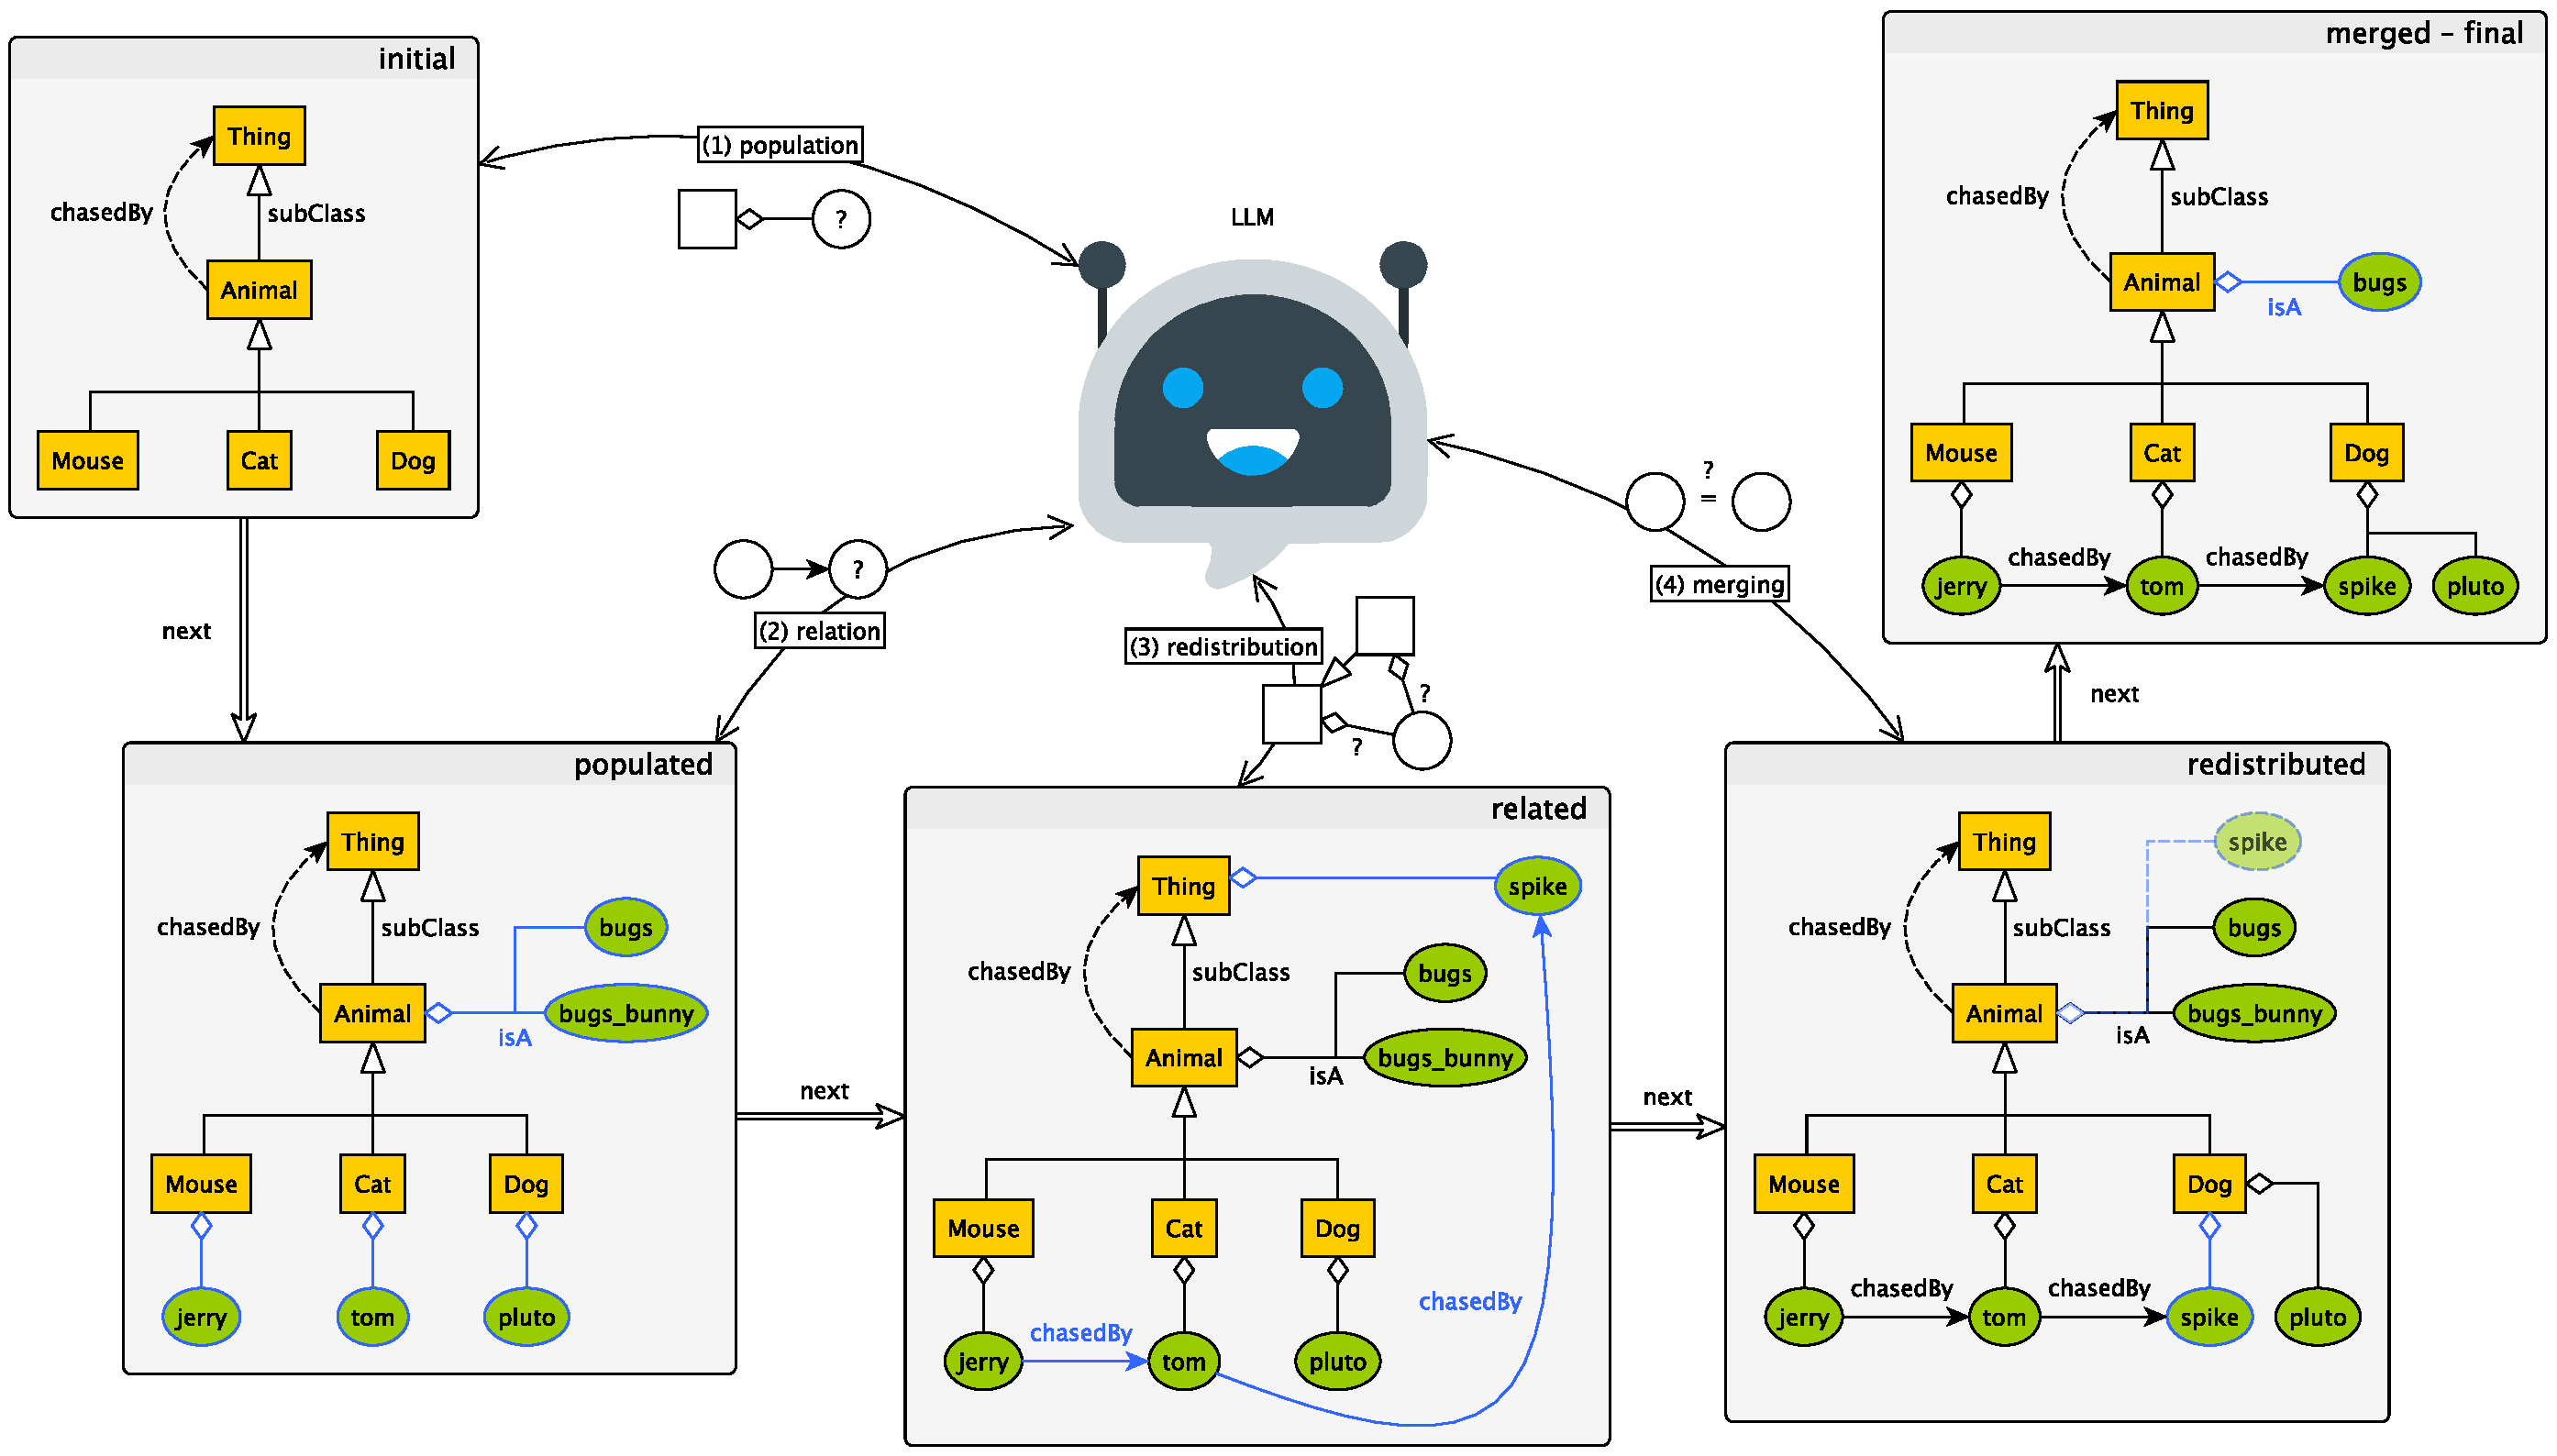
\includegraphics[width=\linewidth]{figures/kgfiller/roadmap}
    \caption[Overview of \llmfkg{}]{%
        Overview of \llmfkg{}, illustrated with a running example.
        %
        The example assumes an ontology about animals, including classes such as $\concept{Cat}$, $\concept{Dog}$, and $\concept{Mouse}$, which are subclasses of $\concept{Animal}$, itself a subclass of $\concept{Thing}$ (\(\top\)).
        %
        Initially, the ontology contains no instances.
        %
        A property $\relation{chasedBy} : \concept{Animal} \times \top$ is defined, indicating that animals can be chased by other entities.
        %
        The figure outlines the four phases of the \llmfkg{} algorithm, with changes highlighted in blue.
    }
    \label{fig:roadmap}
\end{figure}

The \llmfkg{} framework is designed for semi-automatic ontology population, leveraging \glspl{LLM} as oracles.
%
An overview of the \llmfkg{} framework is depicted in \Cref{fig:roadmap}.
%
This section provides a concise yet general description of the framework.

%
\paragraph{Core Functionality}
\label{par:core-functionality}

At its core, \llmfkg{} operates on a partially instantiated ontology.
%
The ontology must include class and property definitions, organized hierarchically as a directed acyclic graph (DAG).
%
Classes may or may not have instances.

%
Class names should be meaningful, concise, and unambiguous to avoid issues during query generation for the \gls{LLM}.
%
The same applies to property names.

%
Given these assumptions, \llmfkg{} generates individuals for all classes and associates them using the ontology's properties.
%
Generated individuals are assigned meaningful names and placed in the most specific class available.

%
The framework supports two primary use cases:
%
\begin{inlinelist}
    \item ontology designers have defined the ontology's structure but lack instances, and
    %
    \item designers want to add more instances to an already populated ontology.
\end{inlinelist}
%
These use cases can be combined, allowing iterative rounds of population and manual refinement.

%
\paragraph{Query Templates}
\label{par:query-templates}

\llmfkg{} relies on query templates to generate questions for the \gls{LLM}.
%
Templates are text strings containing placeholders, which are replaced with actual values during execution.
%
For example, the template \(t = \)\text{``What is the capital of \(\langle c \rangle\)?''} can be instantiated with the substitution \(\sigma = \{\langle c \rangle \mapsto \text{``Italy''}\}\), resulting in \(t / \sigma = \text{``What is the capital of Italy?''}\).

%
We define four types of query templates:
%
\begin{itemize}
    \item \textbf{Individual-seeking templates:} Ask for instances of a class, e.g., ``Examples of \(\langle \text{class} \rangle\)?''.
    %
    \item \textbf{Relation-seeking templates:} Ask for individuals related to a given individual via a property, e.g., ``Examples of \(\langle \text{property} \rangle\) for \(\langle \text{individual} \rangle\)?''.
    %
    \item \textbf{Best-match templates:} Ask for the best class for an individual among candidates, e.g., ``What class is best for \(\langle \text{individual} \rangle\) among \(\langle \text{classes} \rangle\)?''.
    %
    \item \textbf{Individuals-merging templates:} Ask if two instances in a class are identical, e.g., ``In \(\langle \text{class} \rangle\), are \(\langle \text{ind1} \rangle\) and \(\langle \text{ind2} \rangle\) the same?''.
\end{itemize}

%
\paragraph{\gls{LLM} Oracle}
We do not impose constraints on the nature of the \gls{LLM} oracle or the underlying model.
%
\texttt{KGFiller} is agnostic to the specific \gls{LLM} used, as long as it supports generating textual responses from textual prompts.
%
Both prompts and responses are assumed to be strings of arbitrary length, written in a natural language.
%
The natural language must match the one used for naming classes and properties in the ontology.
%
Without loss of generality, we assume this language is English.
%
A key assumption is that the \gls{LLM} oracle is pre-trained on a large corpus of textual data, which includes domain-specific knowledge relevant to the ontology.


\paragraph{Problem Statement}
We formalize the ontology population problem addressed by \texttt{KGFiller} as follows:
%
\begin{enumerate}
    \item A partially instantiated ontology \(\mathcal{O} = \mathcal{C} \cup \mathcal{P} \cup \mathcal{I}\), where:
    %
    \begin{itemize}
        \item \(\mathcal{C} \neq \emptyset\) is a non-empty set of class definitions,
        \item \(\mathcal{P} \neq \emptyset\) is a non-empty set of property definitions, and
        \item \(\mathcal{I}\) is a possibly empty set of individuals and their relationships.
    \end{itemize}
    %
    \item A subsumption relation \(\sqsubseteq\) among the classes in \(\mathcal{C}\).
    %
    \item A set of query templates \(\mathcal{T} = \mathcal{T}_I \cup \mathcal{T}_R \cup \mathcal{T}_B \cup \mathcal{T}_M\), where:
    %
    \begin{itemize}
        \item \(\mathcal{T}_I\) contains individual-seeking templates,
        \item \(\mathcal{T}_R\) contains relation-seeking templates,
        \item \(\mathcal{T}_B\) contains best-match templates, and
        \item \(\mathcal{T}_M\) contains individuals-merging templates.
    \end{itemize}
    %
    \item A trained \gls{LLM} oracle \(\mathcal{L}\), encapsulating domain-specific knowledge.
\end{enumerate}

%

The goal of \texttt{KGFiller} is to generate a set of individuals and relationships \(\mathcal{I}'\) such that \(\mathcal{I} \subseteq \mathcal{I}'\).
%
All new individuals and relationships in \(\mathcal{I}'\) must be consistent with the class and property definitions in \(\mathcal{C}\) and \(\mathcal{P}\), respectively.
%
Specifically:
%
\begin{itemize}
    \item Every individual is associated with the most specific concept in \(\mathcal{C}\) with respect to \(\sqsubseteq\).
    %
    \item For every property in \(\mathcal{P}\), every individual in the property’s domain is associated with one or more individuals in the property’s range.
\end{itemize}


\paragraph{Phases}
To compute \(\mathcal{I}'\), \texttt{KGFiller} executes four sequential phases:
%
\begin{enumerate}
    \item \textbf{Population Phase:} Novel individuals are identified for each class in \(\mathcal{C}\).
    %
    \item \textbf{Relation Phase:} New relationships are identified for each property in \(\mathcal{P}\).
    %
    \item \textbf{Redistribution Phase:} Individuals are redistributed among the classes in \(\mathcal{C}\) to ensure each individual is placed in the most specific class available.
    %
    \item \textbf{Merge Phase:} Semantic duplicates within each class in \(\mathcal{C}\) are detected and merged.
\end{enumerate}
%
The order of these phases is critical.
%
The population phase generates individuals used in the relation phase, which may, in turn, generate additional individuals.
%
The redistribution phase ensures all individuals are placed in the most specific class, while the merge phase reduces semantic duplication.


\paragraph{Ancillary functions}
%
The next section introduces several auxiliary functions used throughout the framework.
%
The function \texttt{GetRange} (resp. \texttt{GetDomain}) retrieves the range (resp. domain) of a given property.
%
The function \texttt{AskOracle} models queries to the \gls{LLM} oracle, accepting and returning arbitrary strings.
%
The function \texttt{ExtractBinary} (resp. \texttt{ExtractNames}) extracts binary values (resp. relevant names of individuals or concepts) from the textual responses of the \gls{LLM}.
%
It returns a Boolean value (resp. a list of names) and accepts a string as input.
%
Finally, the function \texttt{AddToClass} assigns an individual to a class.
%
If the individual is already part of the class or any of its subclasses, the function performs no action.


\subsubsection{Population Phase}
\label{subsubsec:population-phase}
%
\begin{algorithm}
    \captionsetup{font=\algCaptionSize}
    \caption{Populates the given ontology with novel individuals queried from an LLM oracle}
    \label{alg:populate}
    \begin{algorithmic}[1]\algCodeSize
        \Require $\relset{O} = \relset{C} \cup \relset{P} \cup \relset{X}$: partially populated ontology
        \Require $\relset{T}_{I}$: individual seeking query templates
        \Require $\relset{L}$: LLM oracle
        \Require $\concept{R} \in \relset{C}$: root concept to be populated
        \Ensure $\relset{X}'$ contains novel individuals, assigned to the classes in $\relset{C}$
        \medskip
        \Function{\populate}{$\relset{O}, \relset{T}_I, \relset{L}, \concept{R}$}
            \State $\relset{X}' \gets \relset{X}$
            \ForAll{$\concept{C} \in \relset{C} \suchThat \concept{C} \sqsubset \concept{R} \wedge \concept{C} \neq \bot$}
                \State $\relset{O}' \gets \relset{C} \cup \relset{P} \cup \relset{X}'$
                \State $\relset{X}' \gets \Call{\populate}{\relset{O}', \relset{T}_{I}, \relset{L}, \concept{C}}$
            \EndFor
            \ForAll{$\mathit{t} \in \relset{T}_{I}$}
                \State $\mathit{q} \gets \mathit{t}/\{ \var{class} \mapsto \concept{R} \}$
                \State $\mathit{text} \gets \Call{\askOracle}{\relset{L}, \mathit{q}}$
                \ForAll{$\instance{i} \in \Call{\extractNames}{\mathit{text}}$}
                    \State $\relset{O}' \gets \relset{C} \cup \relset{P} \cup \relset{X}'$
                    \State $\relset{X}' \gets \Call{\addToClass}{\relset{O}', \instance{i}, \concept{R}}$
                \EndFor
            \EndFor
            \State \Return $\relset{X}'$
        \EndFunction
    \end{algorithmic}
\end{algorithm}
%
The population phase is based on the \populate{} function, as defined in \Cref{alg:populate}.
%
This function is designed to populate a partially instantiated ontology, denoted as $\relset{O}$, with new instances.
%
It achieves this by querying a \gls{LLM} oracle, represented as $\relset{L}$, using a set of instance-seeking query templates, $\relset{T}_{I}$.


The process begins with a root class $\concept{R} \in \relset{O}$.
%
The function then traverses the class hierarchy defined by the subsumption relation $\sqsubseteq$, following a depth-first post-order strategy.
%
This means that all direct and indirect subclasses of $\concept{R}$ are visited before $\concept{R}$ itself, ensuring that the most specific classes are populated first.
%
Such a strategy is crucial to guarantee that any individual generated during this phase is assigned to the most specific class available.


For each subclass $\concept{C} \sqsubseteq \concept{R}$, the function generates queries by replacing the placeholder $\var{class}$ in each template from $\relset{T}_{I}$ with the name of $\concept{C}$.
%
These queries are then submitted to the \gls{LLM} oracle $\relset{L}$, and the responses are processed to extract the names of the individuals.
%
The number of individuals generated per query is unbounded and depends on the capabilities of the \gls{LLM} oracle $\relset{L}$ and other implementation-specific factors.


It is possible for the same individual to be generated by multiple queries or for multiple subclasses of $\concept{R}$.
%
However, this does not pose any issues, as the \addToClass{} function ensures that individuals are not duplicated and are always assigned to the most specific class.
%
This behavior aligns with the post-order exploration strategy, which prioritizes the population of specific concepts over more general ones.


To populate the entire ontology $\relset{O}$, the function can be invoked with the top class $\top$ as the root:
%
\Call{\populate}{$\relset{O}, \relset{T}_I, \relset{L}, \top$}.
%
This ensures that all classes in $\relset{O}$ are visited and populated systematically.


\subsubsection{Relation Phase}
\label{subsubsec:relation-phase}
%
\begin{algorithm}
    \captionsetup{font=\algCaptionSize}
    \caption{Populates the given ontology with novel relationships queried from an LLM oracle}
    \label{alg:relate}
    \begin{algorithmic}[1]\algCodeSize
        \Require $\relset{O} = \relset{C} \cup \relset{P} \cup \relset{X}$: partially populated ontology
        \Require $\relset{T}_{R}$: relation seeking query templates
        \Require $\relset{L}$: LLM oracle
        \Require $\relation{P} \in \relset{P}$: property to be populated
        \Ensure $\relset{X}'$ contains novel relationships, involving individuals in $\relset{X}$
        \medskip
        \Function{\relate}{$\relset{O}, \relset{T}_R, \relset{L}, \relation{P}$}
            \State $\relset{X}' \gets \relset{X}$
            \State $\concept{D} \gets \Call{\getDomain}{\relation{P}}$
            \State $\concept{R} \gets \Call{\getRange}{\relation{P}}$
            \ForAll{$(\instance{i} : \concept{D}) \in \relset{X}$}
                \ForAll{$\mathit{t} \in \relset{T}_{R}$}
                    \State $\mathit{q} \gets \mathit{t}/\{ \var{individual} \!\mapsto\! \instance{i}, \var{property} \!\mapsto\! \relation{P} \}$
                    \State $\mathit{text} \gets \Call{\askOracle}{\relset{L}, \mathit{q}}$
                    \ForAll{$\instance{i}' \in \Call{\extractNames}{\mathit{text}}$}
                        \State $\relset{O}' \gets \relset{C} \cup \relset{P} \cup \relset{X}'$
                        \State $\relset{X}' \gets \Call{\addToClass}{\relset{O}', \instance{i}', \concept{R}}$
                        \State $\relset{X}' \gets \relset{X}' \cup \{ \relation{P}(\instance{i}, \instance{i}') \}$
                    \EndFor
                \EndFor
            \EndFor
            \State \Return $\relset{X}'$
        \EndFunction
    \end{algorithmic}
\end{algorithm}
%
The relation phase utilizes the \relate{} function to populate a partially instantiated ontology, \(\relset{O}\), with new relationships.
%
These relationships link existing individuals and may introduce novel individuals, based on queries to a \gls{LLM} oracle, \(\relset{L}\), using a set of relation-seeking query templates, \(\relset{T}_{R}\).

%
Consider a property \(\relation{p} \in \relset{O}\), defined as \(\relation{p} : \concept{D} \times \concept{R}\), where \(\concept{D}\) and \(\concept{R}\) represent the domain and range of \(\relation{p}\), respectively.
%
The function queries the \gls{LLM} oracle, \(\relset{L}\), to identify relationships between each individual \(\instance{i} \in \concept{D}\) and potential individuals \(\instance{i}' \in \concept{R}\) through \(\relation{p}\).

%
For each individual \(\instance{i}\) and each query template \(t \in \relset{T}_{R}\), a query \(q\) is generated by substituting placeholders \(\var{property}\) and \(\var{individual}\) in \(t\) with the names of \(\relation{p}\) and \(\instance{i}\), respectively.
%
The query \(q\) is submitted to the \gls{LLM} oracle, and the response is processed to extract the names of individuals to be added to the ontology.
%
Each new individual \(\instance{i}'\) is added to the range \(\concept{R}\) of \(\relation{p}\), along with the relationship \(\relation{p}(\instance{i}, \instance{i}')\).

%
To populate relationships for all properties \(\relation{p} \in \relset{O}\), the function is invoked for each property as follows:
%
\Call{\relate}{$\relset{O}, \relset{T}_R, \relset{L}, \relation{p}$}.

%
It is important to note that the \relate{} function may generate new individuals during its execution.
%
In some cases, the range \(\concept{R}\) of the property \(\relation{p}\) may not be the most specific class for these individuals.
%
For example, a subclass \(\concept{C} \sqsubset \concept{R}\) might better represent some of the generated individuals.
%
This necessitates the redistribution phase, which ensures that all individuals are assigned to the most specific class available.


\subsubsection{Redistribution Phase}
\label{subsubsec:redistribution-phase}
%
\begin{algorithm}
    \captionsetup{font=\algCaptionSize}
    \caption{Redistributes individuals from the given ontology's classes, in such a way that each individual is assigned to the most specific class available}
    \label{alg:redistribute}
    \begin{algorithmic}[1]\algCodeSize
        \Require $\relset{O} = \relset{C} \cup \relset{P} \cup \relset{X}$: partially populated ontology
        \Require $\relset{T}_{B}$: relation seeking query templates
        \Require $\relset{L}$: LLM oracle
        \Require $\concept{R} \in \relset{C}$: root concept within which redistribution should occur
        \Ensure $\relset{X}'$ contains the different assignments of individuals to classes
        \medskip
        \Function{\redistribute}{$\relset{O}, \relset{T}_B, \relset{L}, \concept{R}$}
            \State $\relset{X}' \gets \relset{X}$
            \State $\relset{S} \gets \{ \concept{S} \in \relset{C} \mid \concept{S} \sqsubset \concept{R} \}$
            \ForAll{$(\instance{i} : \concept{R}) \in \relset{X}'$}
                \State $\concept{B} \gets \concept{R}$
                \ForAll{$\mathit{t} \in \relset{T}_{B}$}
                    \State $\mathit{q} \gets \mathit{t}/\{ \var{individual} \mapsto \instance{i}, \var{classes} \mapsto \relset{S} \}$
                    \State $\mathit{text} \gets \Call{\askOracle}{\relset{L}, \mathit{q}}$
                    \ForAll{$\concept{C} \in \Call{\extractNames}{\mathit{text}}$}
                        \State $\concept{B} \gets \concept{C}$
                        \State \Break{going to line \ref{line:first-result}}
                    \EndFor
                \EndFor
                \State $\relset{O}' \gets \relset{C} \cup \relset{P} \cup \relset{X}'$ \label{line:first-result}
                \State $\relset{X}' \gets \Call{\addToClass}{\relset{O}', \instance{i}, \concept{B}}$
            \EndFor
            \ForAll{$\concept{C} \in \relset{C} \suchThat \concept{C} \sqsubset \concept{R} \wedge \concept{C} \neq \bot$}
                \State $\relset{O}' \gets \relset{C} \cup \relset{P} \cup \relset{X}'$
                \State $\relset{X}' \gets \Call{\redistribute}{\relset{O}', \relset{T}_{B}, \relset{L}, \concept{C}}$
            \EndFor
            \State \Return $\relset{X}'$
        \EndFunction
    \end{algorithmic}
\end{algorithm}
%
The redistribution phase utilizes the \redistribute{} function, as defined in \Cref{alg:redistribute}.
%
This function redistributes individuals among the classes of an instantiated ontology, \(\relset{O}\), ensuring that each individual is assigned to the most specific class available.
%
To achieve this, the function queries the \gls{LLM} oracle, \(\relset{L}\), using a set of best-match query templates, \(\relset{T}_{B}\).

%
Starting from a root class \(\concept{R} \in \relset{O}\), the function recursively explores the class hierarchy defined by the subsumption relation \(\sqsubseteq\).
%
It follows a depth-first pre-order traversal strategy, visiting each class before its subclasses.
%
This approach ensures that individuals can be reassigned to more specific classes as the traversal progresses.

%
For each visited class \(\concept{C} \sqsubseteq \concept{R}\), the function evaluates whether \(\concept{C}\) is the most appropriate class for all individuals currently assigned to it.
%
If a more specific subclass of \(\concept{C}\) is better suited for an individual, the function reassigns the individual accordingly.
%
For example, if \(\concept{Cat} \sqsubset \concept{Animal}\) and an individual \(\instance{tom}\) is initially assigned to \(\concept{Animal}\), the function reassigns \(\instance{tom}\) to \(\concept{Cat}\).

%
To determine the best class for an individual \(\instance{i} : \concept{C}\), the function generates a query for each template \(t \in \relset{T}_{B}\).
%
The placeholders \(\var{individual}\) and \(\var{classes}\) in \(t\) are replaced with the name of \(\instance{i}\) and the concatenated names of all direct subclasses of \(\concept{C}\), respectively.
%
The resulting query is submitted to the \gls{LLM} oracle, and the response is processed to extract candidate class names.
%
The first class in the response is selected as the best match, and \(\instance{i}\) is reassigned to it.

%
Since the function is recursive, an individual may be reassigned multiple times until it reaches the most specific class available in the ontology.
%
The depth-first pre-order strategy is crucial for this process, as it allows individuals to ``move down'' the class hierarchy efficiently while keeping query sizes manageable.

%
To redistribute all individuals in an ontology, the function can be invoked with the top class \(\top\) as the root:
%
\Call{\redistribute}{$\relset{O}, \relset{T}_{B}, \relset{L}, \top$}.
%
This ensures that every individual in \(\relset{O}\) is assessed and reassigned to the most specific class, if necessary.


\subsubsection{Merge Phase}
\label{subsubsec:merge-phase}
%
\begin{algorithm}
    \captionsetup{font=\algCaptionSize}
    \caption{Merges syntactically and semantically similar individuals from the given ontology's classes}
    \label{alg:merge}
    \begin{algorithmic}[1]\algCodeSize
        \Require $\relset{O} = \relset{C} \cup \relset{P} \cup \relset{X}$: partially populated ontology
        \Require $\relset{T}_{M}$: indivuals merging query templates
        \Require $\relset{L}$: LLM oracle
        \Require $\concept{R} \in \relset{C}$: root concept within which merge should occur
        \Ensure $\relset{X}'$ contains no duplicated individuals
        \medskip
        \Function{\merge}{$\relset{O}, \relset{T}_{M}, \relset{L}, \concept{R}$}
            \State $\relset{X}' \gets \relset{X}$
            \ForAll{$\concept{C} \in \relset{C} \suchThat \concept{C} \sqsubset \concept{R}$}
                \State $\mathcal{D} \gets \emptyset$
                \ForAll{$\instance{i}, \instance{j} : \concept{C} \suchThat ( \instance{i}, \instance{j} ) \in \relset{X}' \times \relset{X}'$}
                    \If{$\Call{\synSimilar}{\instance{i}, \instance{j}}$}
                        \State $\mathcal{D} \gets \mathcal{D} \cup \{\{\instance{i}, \instance{j}\}\}$
                    \EndIf
                \EndFor
                \ForAll{$\{ \instance{i}, \instance{j} \} \in \mathcal{D}$}
                    \ForAll{$\mathit{t} \in \relset{T}_{M}$}
                    \label{line:next-couple}
                        \State $\mathit{q} \gets \mathit{t}/\{ \var{ind_1}\!\mapsto\!\instance{i}, \var{ind_2}\!\mapsto\!\instance{j},
                            \var{class}\!\mapsto\!\concept{C} \}$
                        \State $\mathit{text} \gets \Call{\askOracle}{\relset{L}, \mathit{q}}$
                        \If{$\Call{\extractBinary}{text}$}
                            \State $\relset{X}' \gets \Call{\mergeInst}{i, j}$
                            \State \Break{going to line \ref{line:next-couple}}
                        \EndIf
                    \EndFor
                \EndFor
            \EndFor
        \EndFunction
    \end{algorithmic}
\end{algorithm}

%
The \merge{} function is responsible for identifying and merging duplicated individuals in an instantiated ontology, denoted as $\relset{O}$.
%
Duplicated individuals are defined as those with slightly different names but representing the same semantic entity.
%
Such duplicates often arise as a by-product of earlier phases in the ontology population process.


For example, consider the individuals $\instance{maincoone\_cat}$ and $\instance{maincoone}$, both belonging to the class $\concept{Cat} \sqsubset \concept{Animal}$.
%
Although their names differ syntactically, they refer to the same entity.
%
To address this, the \merge{} function queries the \gls{LLM} oracle, denoted as $\relset{L}$, to identify semantically similar individuals and merge them into a single entity.


The \merge{} function operates by scanning the ontology $\relset{O}$ for pairs of syntactically similar individuals.
%
For each pair, it uses a set of merging query templates, $\relset{T}_{M}$, to query the \gls{LLM} oracle.
%
The oracle's response determines whether the individuals should be merged.


The process begins with a root class $\concept{R} \in \relset{O}$ and recursively explores the class hierarchy defined by the subsumption relation $\sqsubseteq$.
%
For each class $\concept{C} \sqsubseteq \concept{R}$, the function identifies a set $\mathcal{D}$ of candidate duplicate pairs using the \synSimilar{} function.
%
Each pair is then evaluated using the \extractBinary{} function, which interprets the oracle's response as a Boolean value.
%
If the response is positive, the \mergeInst{} function is invoked to merge the individuals.
%
This involves transferring all information from one individual to the other and removing the redundant individual, resulting in an updated ontology $\relset{X}'$.


The merging process relies on templates in $\relset{T}_{M}$.
%
For each candidate pair, a query is generated by replacing the placeholders $\var{ind\_1}$, $\var{ind\_2}$, and $\var{class}$ in the template with the names of the individuals and the class $\concept{C}$, respectively.
%
The first template yielding a positive response is considered definitive, and further templates are not queried.
%
To ensure deterministic behavior and avoid issues arising from the oracle's creativity, the temperature parameter is set to 0.0 during these queries.


To detect and merge all duplicated individuals in an ontology $\relset{O}$, the function can be invoked as follows:
%
\Call{\merge}{$\relset{O}, \relset{T}_M, \relset{L}, \top$}.
%
This ensures that all classes in $\relset{O}$ are systematically visited, and any semantic duplicates are resolved.


\paragraph{Remarks}
%
\Cref{alg:merge} employs a post-order exploration strategy.
%
However, the choice of exploration strategy is \emph{not} critical for the merging phase.
%
Alternative strategies can be used, provided they visit all direct and indirect subclasses of $\concept{R}$.

%
The \synSimilar{} function plays a crucial role in determining whether two instances, $\instance{i}$ and $\instance{j}$, are sufficiently similar to be considered for merging.
%
Its implementation significantly impacts the overall performance of the \merge{} function.
%
% For example, one could define similarity based on shared substrings longer than a threshold $\lambda$.
% %
% Empirically, $\lambda$ can be set to 4 characters.

%
Regarding the merging phase, one might question why entity alignment approaches~\cite{ZhaoTkde2022} are not used.
%
While effective for identifying similar instances across different \glspl{KG}, these methods typically require additional domain-specific data~\cite{ChenIjcai2018,XuAcl2019}.
%
This is because entity alignment systems rely on ad-hoc \gls{ML} models trained for the alignment task, introducing extra complexity.

%
In contrast, our approach leverages the same \gls{LLM} oracle for both ontology population and duplicate identification.
%
Although not entirely error-free, this method avoids additional computational overhead during the population phase.
%
It also eliminates the need for users to provide extra domain-specific data or train additional models, simplifying the overall process.
%



\subsection{Case Study and Experiments}
\label{subsec:case-study}
%
This section presents a case study designed to empirically validate \llmfkg{}.

%
\subsubsection{Experimental Setup}
\label{subsubsec:experimental-setup}
%
The experimental setup involves designing a non-trivial ontology, as detailed in \Cref{subsubsec:kgfiller-ontology}.
%
The ontology includes a class hierarchy and a set of properties, which are populated using \llmfkg{}.
%
We fine-tune specific query templates (\Cref{subsubsec:query-templates}) and utilize various \glspl{LLM} from different families and technologies (\Cref{subsubsec:llms-oracles}).
%
This process generates a set of populated ontologies, all sharing the same structure but differing in their content.
%
The populated ontologies are analyzed and compared to evaluate the performance of \llmfkg{} and the impact of the chosen \gls{LLM} on the quality of the population process.
%
To achieve this, we define a taxonomy of errors and a set of metrics (\Cref{subsec:performance-metrics}) to measure the quality of the generated ontologies.
%
The evaluation is performed through a manual inspection of the populated ontologies, examining each individual and relationship (\Cref{subsec:results}).

%
Testing \llmfkg{} on a custom ontology, rather than a publicly available one, offers several advantages.
%
First, it allows precise control over the experiment's complexity and content.
%
Second, it avoids potential biases where \glspl{LLM} perform well due to prior exposure to the ontology during training.
%
However, this approach lacks ground truth data, making automatic validation infeasible.
%
Thus, manual inspection is necessary to identify errors and ensure the correctness of the algorithm's output.

%
\subsubsection{Code and Data}
\label{subsubsec:code-and-data}
%
The experiments are conducted using a Python implementation of \llmfkg{}, which is publicly available on GitHub\footnote{\url{https://github.com/Chistera4-Expectation/kg-filler}}.
%
The experimental results are also available on a dedicated repository\footnote{\url{https://github.com/Chistera4-Expectation/knowledge-graphs/branches}}, where each Git branch corresponds to a specific experiment.
%
The \texttt{main} branch contains the initial ontology, which includes only class and property definitions without any individuals.

%
For reproducibility, each experiment branch includes the populated ontology and the cache of query--response pairs from the \gls{LLM}.
%
This allows others to inspect the exact queries and responses and reproduce the experiments deterministically.
%
Additionally, the experiments are automated, with each commit in the branch corresponding to a single operation performed by \llmfkg{} (e.g., populating a class or property).
%
This commit history provides a detailed sequence of operations for each experiment.

%
\subsubsection{Ontology}
\label{subsubsec:kgfiller-ontology}
%
\begin{figure*}
    \centering
    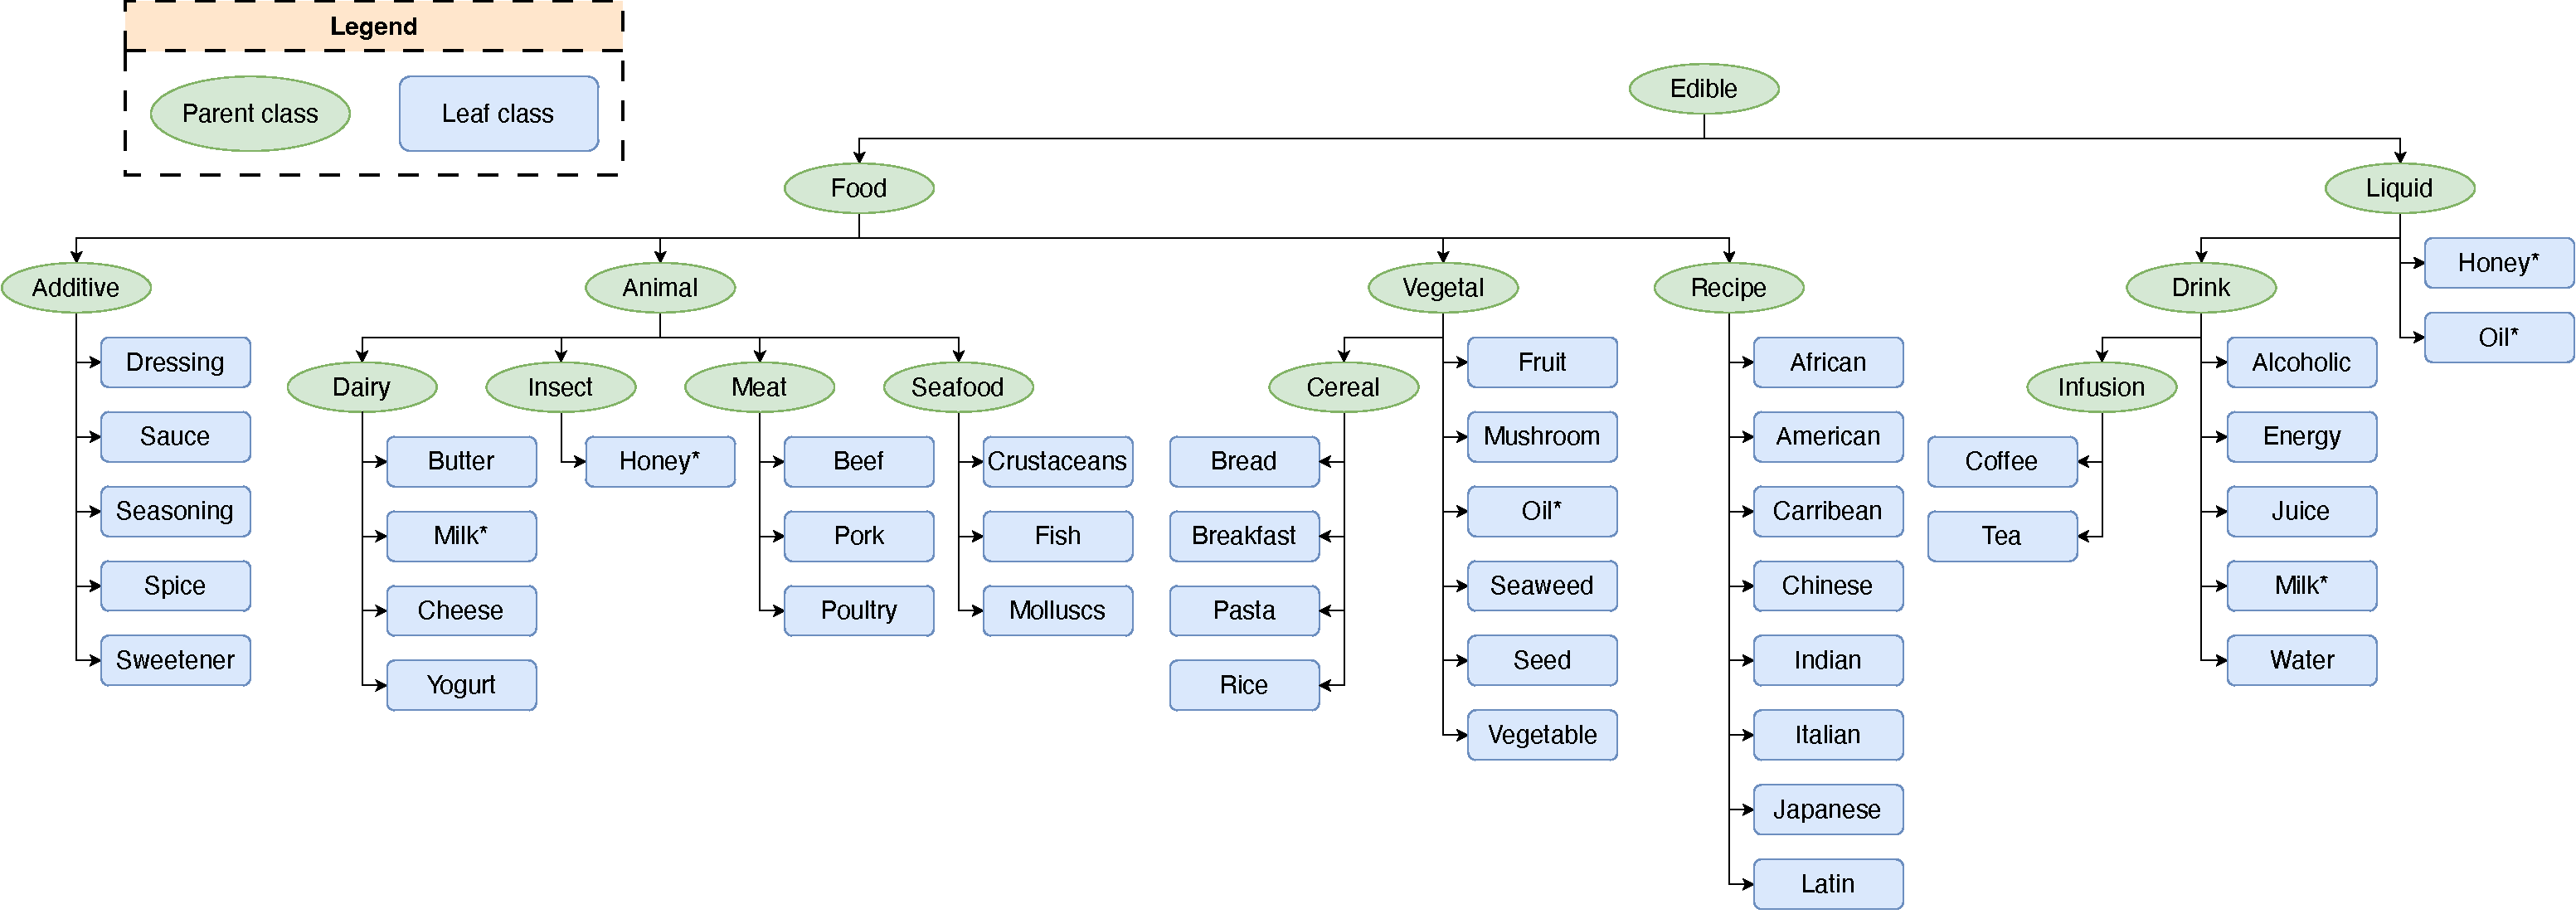
\includegraphics[width=\linewidth]{figures/kgfiller/ontology-skeleton}
    \caption[Class hierarchy of the ontology used in the experiments]{
        %
        Class hierarchy of the case study ontology.
        %
        Notice that the hierarchy is not really a tree, but rather a \gls{DAG}.
        %
        The asterisk (*) denotes classes having multiple super-classes (they are depicted once per super-class for the sake of readability).
    }
    \label{fig:ontology}
\end{figure*}
%
The ontology is designed in the \emph{nutritional} domain, as required by the \expectation{} project~\cite{expectation-extraamas2021}.
%
In \expectation{}, the ontology serves as the foundation for a nutritional recommender system, which suggests recipes based on users' dietary needs and preferences~\cite{DBLP:journals/cmpb/MagniniCCAO23}.
%
Although the recommender system is outside the scope of this work, this context helps clarify the ontology design choices.

%
The ontology focuses on representing \emph{recipes} and their \emph{ingredients}.
%
It categorizes \emph{edible} items into several subclasses to accommodate diverse dietary requirements and preferences.
%
\Cref{fig:ontology} illustrates the class hierarchy, which is structured as a directed acyclic graph (DAG).
%
The root class is \concept{Edible}, with subclasses such as \concept{Recipe}, which further branches into various cuisines (e.g., \concept{Italian}, \concept{Chinese}).

%
Some classes include an annotation property, \relation{fancyName}, to provide a more descriptive label for the class.
%
Another key property is $\relation{ingredientOf} : \concept{Edible} \times \concept{Recipe}$, which links recipes to their ingredients.
%
Initially, the ontology is a skeleton containing no individuals.

%
\subsubsection{Query Templates}
\label{subsubsec:query-templates}
%
To query the \gls{LLM} oracle, we define and fine-tune specific query templates.

%
The set of individual-seeking templates, $\relset{T}_{I}$, is defined as:
%
\str{$ ( $instances$ \mid $examples$ ) $ list for class $\var{class} ( $, names only$ )? $}.
%
Here, $(A|B)$ denotes two template variants, one with $A$ and one with $B$, while $(A)?$ indicates optional inclusion of $A$.

%
The set of relation-seeking templates, $\relset{T}_{R}$, includes:
%
\str{ingredient list for $\var{individual}$, names only}.
%
This template uses a hard-coded property name for natural phrasing.

%
The set of best-match templates, $\relset{T}_{B}$, is defined as:
%
\str{most adequate class for $\var{individual}$ among: $\var{classes}$. concise}.

%
Finally, the set of individual-merging templates, $\relset{T}_{M}$, is:
%
\str{in the $\var{class}$ class, should instances $\var{ind_1}$ and $\var{ind_2}$ be merged together as semantic and ontologic duplicates? yes or no answer only}.

%
\subsubsection{\gls{LLM} Oracles}
\label{subsubsec:llms-oracles}
%
To evaluate the impact of \gls{LLM} quality on \llmfkg{}, we integrate several state-of-the-art \glspl{LLM}.
%
These include both open-source models (e.g., OpenChat, Llama) and closed-source models (e.g., GPT), as well as \gls{MoE} models like Mixtral.

%
Open-source models are queried using the Hugging Chat API\footnote{\url{https://github.com/Soulter/hugging-chat-api}}, a third-party library for the HuggingFace platform\footnote{\url{https://huggingface.co}}.
%
This API supports multiple simultaneous conversations with different \glspl{LLM}.
%
The selected open-source models include:
%
\begin{description}
    \item[Llama 2:] A family of open-source \glspl{LLM}, with the 70 billion parameters model used in our experiments~\cite{llama2-2023}.
    %
    \item[OpenChat 3.5:] A 13 billion parameters model fine-tuned from the Llama family, optimized for mixed-quality data~\cite{wang2023openchat}.
    %
    \item[Mistral 7B:] A 7 billion parameters model, designed for high performance relative to its size~\cite{mistral}.
    %
    \item[Gemma:] A lightweight model from Google, based on the Gemini research~\cite{gemini}.
\end{description}

%
For \gls{MoE} models, we include:
%
\begin{description}
    \item[Mixtral:] A sparse \gls{MoE} aggregating eight 7 billion parameters models~\cite{mixtral}.
    %
    \item[Nous Hermes:] A flagship model trained on high-quality data, including GPT-4 outputs.
\end{description}

%
Closed-source models are queried using the OpenAI API\footnote{\url{https://openai.com/blog/openai-api}}.
%
The selected models include:
%
\begin{description}
    \item[GPT 3.5 Turbo:] A widely used model with significant performance improvements~\cite{gpt3-2020}.
    %
    \item[GPT 4 Turbo:] The latest version, reported to be a \gls{MoE}~\cite{gpt4}.
\end{description}

%
\Cref{tab:llms_sizes} summarizes the \glspl{LLM} used, their sizes, and relevant hyperparameters.
%
The size of the \gls{LLM} significantly impacts its performance, with GPT-4 being nearly 200 times larger than the largest open-source model (Llama 2).
%
This size difference is expected to influence the quality of the constructed ontology, as discussed in \Cref{subsec:results}.

\begin{table}
    \caption[LLMs sizes and setup]{%
        Size (number of parameters) and experiments setup of the different LLMs used in \llmfkg{}.
        Values reported with $^{\ast}$ are an educated estimate
        -- not confirmed --,
        as the corresponding models have not be fully disclosed to the public.
    }
    \resizebox{\columnwidth}{!}{
    \centering
    \begin{tabular}{l | c c c c c} \toprule
        LLM & size [B] & max tokens & max retries & back-off time [s] & temperature \\ \midrule
        GPT 3.5 Turbo~\cite{gpt3-2020} & 375$^{\ast}$ & 1000 & 2 & 30 & 0.7 \\
        GPT 4 Turbo~\cite{gpt4} & 1500$^{\ast}$ & 1000 & 2 & 30 & 0.7 \\ \midrule
        Openchat~\cite{wang2023openchat} & 13 & 1000 & 2 & 30 & 0.1 \\
        Llama2~\cite{llama2} & 70 & 1000 & 2 & 30 & 0.1 \\
        Mistral~\cite{mistral} & 7 & 1000 & 2 & 30 & 0.1 \\
        Gemma~\cite{gemini} & 7 & 1000 & 2 & 30 & 0.1 \\ \midrule
        Mixtral~\cite{mixtral} & 56 & 1000 & 2 & 30 & 0.1 \\
        Nous Hermes & 56 & 1000 & 2 & 30 & 0.1 \\ \bottomrule
    \end{tabular}
    }
    \label{tab:llms_sizes}
\end{table}


\subsection{Performance Metrics}
\label{subsec:performance-metrics}
%
Evaluating the quality of ontology construction and population processes is challenging.
%
This is due to the interplay of various factors, such as the quality of the generated instances and the validity of the relationships.
%
In this section, we outline the potential issues in the \llmfkg{} framework and define corresponding quantitative performance metrics.


\subsubsection{Types of Errors}
\label{subsubsec:error_types}
%
When using sub-symbolic black-box models, such as \glspl{LLM}, for ontology population, several types of errors may arise.
%
These errors depend on the quality of the oracle's output and the robustness of the post-processing procedure.
%
\glspl{LLM} are prone to hallucinations, which can lead to unreliable suggestions.
%
Additionally, the structure of their output is often unpredictable, making post-processing complex and error-prone.
%
We categorize the errors as follows:

%
\paragraph{Misplacement Error (\(E_{\text{mis}}\))}

This error occurs when an individual is added to the ontology but assigned to the wrong class.
%
It is common in large ontologies with many classes.
%
We distinguish between two cases:
%
\begin{inlinelist}
    \item the individual is assigned to a class that is too general, where a more specific subclass exists, and
    %
    \item the individual is assigned to a semantically incorrect class.
\end{inlinelist}
%
While both cases are treated equally in our analysis, the first represents a lack of precision, whereas the second is a more severe semantic issue.

%
\paragraph{Incorrect Individual (\(E_{\text{ii}}\))}

This error arises when an individual is added to the ontology but is irrelevant to its context, despite having a meaningful name.
%
Such errors may result from:
%
\begin{inlinelist}
    \item hallucinated responses from the \gls{LLM}, suggesting out-of-scope instances, or
    %
    \item incorrect post-processing of valid \gls{LLM} outputs.
\end{inlinelist}
%
For example, the \gls{LLM} might suggest that ``\emph{dog}'' is an instance of the class ``\emph{Edible meat}''.

%
\paragraph{Meaningless Individual (\(E_{\text{mi}}\))}

This error occurs when the name of an individual is nonsensical and should not be part of the ontology.
%
It often results from the failure to interpret negative responses or to correctly extract valid instances from the \gls{LLM} output.
%
For instance, failing to recognize a response like ``\emph{I do not have access to such data}'' as negative could lead to meaningless entries.

%
\paragraph{Class-Like Individuals (\(E_{\text{ci}}\))}

These errors occur when an individual has the same or a very similar semantic meaning as the class it belongs to.
%
This often happens due to overly broad responses from the \gls{LLM}.
%
For example, querying for ``\emph{meat}'' instances might result in the \gls{LLM} suggesting ``\emph{meat}'' as an individual of the class ``\emph{Meat}''.

%
\paragraph{Duplicate Individuals (\(E_{\text{di}}\))}

Duplicate individuals are semantically identical or very similar entries in the ontology.
%
They may arise from:
%
\begin{inlinelist}
    \item repeated suggestions by the \gls{LLM}, or
    %
    \item errors in post-processing.
\end{inlinelist}
%
The iterative nature of the ontology population process can also lead to duplicates.
%
The \emph{merge phase} of \llmfkg{} aims to address this issue by identifying and merging duplicates, but errors may still persist.

%
\paragraph{Wrong Relation (\(E_{\text{wr}}\))}

This error occurs when a relationship between two individuals is invalid.
%
During the relation phase, \llmfkg{} queries the \gls{LLM} to populate relationships.
%
However, hallucinated responses can lead to incorrect relationships.
%
For example, the \gls{LLM} might suggest that ``\emph{onions}'' are an ingredient of ``\emph{carbonara spaghetti},'' which is inconsistent with the ontology.

%
\paragraph*{On Subjectivity}

The identification of these errors involves a degree of subjectivity, particularly for \(E_{\text{ii}}\) and \(E_{\text{wr}}\).
%
To mitigate this, multiple evaluators independently assess the ontology, and disagreements are resolved through majority voting.

%
\subsubsection{Measures}
\label{subsubsec:measures}

To assess the quality of the ontology population process, we define the following metrics:

%
\begin{enumerate}
    \item The total number of generated individuals, \(\mathit{TI}\), which evaluates the ability of \llmfkg{} to generate diverse instances.
    %
    \item The minimum and maximum class weights, \(\mathit{minCW}\) and \(\mathit{maxCW}\), representing the smallest and largest number of individuals per class, respectively.
    %
    \item The total number of individuals in leaf classes, \(\mathit{TL}\), which measures the specificity of the generated instances.
    %
    \item The total number of individuals affected by errors, \(\mathit{TE}\), where each individual is counted once, regardless of the number of errors.
    %
    \item The relative individual error, \(\mathit{RIE}\), defined as:
    %
    \begin{equation}
        \label{eq:relative_individual_error}
        \mathit{RIE} = \frac{\mathit{TE}}{\mathit{TI}}.
    \end{equation}
    %
    \item The total number of errors for each error type, as defined in \Cref{subsubsec:error_types}.
    %
    \item The total number of generated relationships, \(\mathit{TR}\).
    %
    \item The relative relation error, \(\mathit{RRE}\), defined as:
    %
    \begin{equation}
        \label{eq:relative_relation_error}
        \mathit{RRE} = \frac{E_{\text{wr}}}{\mathit{TR}}.
    \end{equation}
\end{enumerate}

%
Finally, we define an overall quality metric, \(Q\), which summarizes the correctness of the ontology:
%
\begin{equation}
    \label{eq:quality_metric}
    Q = \frac{\mathit{TI} - \mathit{TE} + \mathit{TR} - E_{\text{wr}}}{\mathit{TI} + \mathit{TR}}.
\end{equation}
%
This metric ranges from 0 (all data is invalid) to 1 (all data is valid).

%
\subsubsection{Quality of Service}

To evaluate the quality of service (QoS) of the \gls{LLM} oracle, we consider the following metrics:

%
\begin{itemize}
    \item The time required to populate the ontology, \(\Delta t\), measured as the difference between the first and last query timestamps.
    %
    \item The total number of queries, \(N\), submitted to the \gls{LLM}, including inconclusive ones.
    %
    \item The total cost, \(\$\), in USD, of a single \llmfkg{} run, considering cached queries.
\end{itemize}

%
These metrics are influenced by factors such as network latency, response length, and the pricing scheme of the \gls{LLM} provider.
%
At the time of writing, Hugging Face models are free but rate-limited, while OpenAI models have the following costs:
%
\begin{description}
    \item[GPT 3.5 Turbo:] \$0.5 (input) and \$1.5 (output) per million tokens.
    %
    \item[GPT 4 Turbo:] \$10 (input) and \$30 (output) per million tokens.
\end{description}
%


\subsection{Results}
\label{subsec:results}
%
\begin{table*}
    \caption[Performance of \llmfkg{} over different state-of-the-art LLMs]{
        Performance of \llmfkg{} over different state-of-the-art LLMs.
        For each performance metric (column) we denote with $^{\dag}$ and $^{\ddag}$
        the best and second best performing model respectively.
    }
    \resizebox{\textwidth}{!}{
    \centering
    \begin{tabular}{l | c c c c c c c c c c c c c c | c} \toprule
        LLM & $\mathit{TI}$ & $\mathit{minCW}$ & $\mathit{maxCW}$ & $\mathit{TL}$ & $\mathit{TE}$ & $\mathit{RIE}$ & $E_{mis}$ & $E_{ii}$ & $E_{mi}$ & $E_{ci}$ & $E_{di}$ & $\mathit{TR}$ & $E_{wr}$ & $\mathit{RRE}$ & $Q$
        \\ \midrule
        GPT 3.5 Turbo~\cite{gpt3-2020} & 511 & 4 & 40 & 495 & 44$^{\dag}$ & 0.0861$^{\dag}$ & 37$^{\dag}$ & 1$^{\dag}$ & 0$^{\dag}$ & 13$^{\dag}$ & 3$^{\dag}$ & 736 & 51$^{\dag}$ & 0.0693$^{\dag}$ & 0.924$^{\dag}$
        \\
        GPT 4 Turbo~\cite{gpt4} & 735 & 5 & 56 & 727 & 91$^{\ddag}$ & 0.1238 & 40$^{\ddag}$ & 5 & 18 & 19 & 8 & 1061 & 96$^{\ddag}$ & 0.0905$^{\ddag}$ & 0.896$^{\ddag}$ 
        \\ \midrule
        Openchat~\cite{wang2023openchat} & 997 & 9 & 105 & 970 & 244 & 0.2447 & 105 & 65 & 11 & 23 & 32 & 1329$^{\dag}$ & 440 & 0.3311 & 0.706 
        \\
        Llama2~\cite{llama2} & 665 & 6 & 55 & 609 & 119 & 0.1789 & 84 & 8 & 4$^{\ddag}$ & 21 & 7 & 1062 & 197 & 0.1855 & 0.817
        \\
        Mistral~\cite{mistral} & 1176$^{\dag}$ & 11$^{\dag}$ & 110 & 1113$^{\dag}$ & 255 & 0.2168 & 133 & 14 & 60 & 32 & 72 & 1211 & 284 & 0.2345 & 0.774 
        \\
        Gemma~\cite{gemini} & 433 & 1 & 40 & 407 & 107 & 0.2471 & 70 & 2$^{\ddag}$ & 21 & 16$^{\ddag}$ & 3$^{\dag}$ & 989 & 290 & 0.2932 & 0.721 
        \\ \midrule
        Mixtral~\cite{mixtral} & 841 & 3 & 111$^{\ddag}$ & 819 & 228 & 0.2711 & 94 & 22 & 78 & 22 & 15 & 960 & 174 & 0.1813 & 0.777 
        \\
        Nous Hermes & 1121$^{\ddag}$ & 11$^{\dag}$ & 121$^{\dag}$ & 1082$^{\ddag}$ & 123 & 0.1097$^{\ddag}$ & 59 & 12 & 11 & 28 & 11 & 1222$^{\ddag}$ & 227 & 0.1858 & 0.851 
        \\ \bottomrule
    \end{tabular}
    }
    \label{tab:performance}
\end{table*}
%
\Cref{tab:performance} summarizes the results obtained from different runs of \llmfkg{}, supported by the various \glspl{LLM} discussed in \Cref{subsubsec:llms-oracles}.
%
Overall, the results demonstrate the feasibility of constructing ontologies by leveraging the implicit knowledge embedded in \glspl{LLM} during their training.
%
Focusing on the quality metric \(Q\), at least \(75\%\) of the instances and relations added to the initial empty ontology are valid for most of the evaluated \glspl{LLM}.
%
For instance, GPT 3.5 Turbo achieves \(92.4\%\) valid instances and relations, while its successor, GPT 4 Turbo, achieves a comparable performance with \(Q = 89.6\%\).
%
These findings highlight the reliability of the proposed approach.

The analysis of error types during the ontology population phase provides additional insights.
%
Most errors are related to the relative positioning of added instances rather than the inclusion of nonsensical entries.
%
This observation reinforces the potential of \glspl{LLM} to extract structured and precise knowledge for specific domains, such as the food domain in this case study.

Different models excel in different performance metrics.
%
For example, the \emph{Mistral} model constructs one of the largest ontologies, adding 1176 instances and 1211 relations.
%
However, the large size of the ontology introduces quality issues, resulting in a high relative error rate.
%
In contrast, GPT-based models achieve lower relative error rates, with GPT 3.5 Turbo achieving a relative individual error of \(0.0861\) and a relative relation error of \(0.0693\).
%
Despite this, GPT-based models tend to produce smaller ontologies, with the GPT 3.5 Turbo version containing nearly half the instances of other models.

When minimizing erroneous instances and relations, GPT-based solutions, particularly GPT 3.5, emerge as the most effective.
%
The significant size difference between GPT-based models and their counterparts provides an advantage in handling complex tasks, such as classifying instances into semantic classes or listing recipe ingredients without hallucinations or inaccuracies.
%
Ontologies constructed using the GPT family exhibit the fewest critical mistakes or hallucinations (see \Cref{subsubsec:interesting_samples}).

Nevertheless, the results also indicate that closed-source models are not the only viable option.
%
Some open-source models achieve comparable performance levels.
%
For instance, the \emph{Llama 2} model constructs a smaller but effective ontology, maintaining low counts of incorrect (\(E_{\text{ii}}\)) and meaningless (\(E_{\text{mi}}\)) individuals, thereby demonstrating its potential.

Additionally, the \emph{Nous Hermes} model, leveraging the \gls{MoE} process, constructs a large ontology—nearly twice the size of the GPT 3.5 version.
%
It achieves nearly \(90\%\) correctness for added individuals, surpassing GPT 4 Turbo, with an overall quality metric of \(Q = 85.1\%\).
%
These results confirm the correlation between the dimensionality of \glspl{LLM} and the quality of the constructed ontology, as \emph{Llama 2} and \emph{Nous Hermes} are among the largest open-source models (see \Cref{tab:llms_sizes}).

A strong proportionality is observed between the relative individual error (\(\mathit{RIE}\)) and the relative relation error (\(\mathit{RRE}\)).
%
Models achieving low \(\mathit{RIE}\) also tend to achieve low \(\mathit{RRE}\).
%
This suggests that the ability of \glspl{LLM} to suggest instances for specific classes or classify random instances correctly is proportional to their ability to establish valid relationships between instances without proposing meaningless associations.
%
This finding underscores the general capability of \glspl{LLM} to handle both instances and relationships in ontology construction.


\paragraph{\Gls{QoS}-Related Remarks}
%
\begin{table}
    \caption[\llmfkg{} \gls{QoS} measurements]{%
        \Gls{QoS} measurements (duration, number of queries, cost) of \llmfkg{} over different state-of-the-art LLMs.
        Each line describes the \gls{QoS} of the experiment corresponding to the same line in \Cref{tab:performance}.
    }
    % \resizebox{\linewidth}{!}{
    \centering
    \begin{tabular}{l | c c c} \toprule
        LLM & $\mathit{\Delta t}$ & $\mathit{N}$ & $\$$
        \\ \midrule
        GPT 3.5 Turbo~\cite{gpt3-2020} & 15m 39s & 1236 & 0.06
        \\
        GPT 4 Turbo~\cite{gpt4} & 58m 43s & 2414 & 2.16
        \\ \midrule
        Openchat~\cite{wang2023openchat} & 11h 50m 25s & 4710 & n.a.
        \\
        Llama2~\cite{llama2} & 5h 8m28s & 1990 & n.a.
        \\
        Mistral~\cite{mistral} & 2h 19m 40s & 907 & n.a.
        \\
        Gemma~\cite{gemini} & 4h 55m 2s & 1141 & n.a.
        \\ \midrule
        Mixtral~\cite{mixtral} & 12h 51m 2s & 2620 & n.a.
        \\
        Nous Hermes & 14h 40m 3s & 6083 & n.a.
        \\ \bottomrule
    \end{tabular}
    % }
    \label{tab:kgfiller-qos}
\end{table}
%
\Cref{tab:kgfiller-qos} summarizes the \gls{QoS} measurements from the experiments.
%
GPT-based models generally exhibit faster execution times (\(\Delta t\)), primarily due to the looser rate limitations applied by OpenAI for paying users.
%
However, this comes at the cost of moderate expenses in USD (\(\$\)).
%
In contrast, models accessible via the Hugging Face API are free to use but subject to stricter rate limitations, resulting in longer execution times for \llmfkg{}.

The total number of queries (\(N\)) varies significantly across runs, depending on the \gls{LLM} model.
%
Given that all models were subject to the same length limitations, this variability likely stems from differences in the verbosity of the \glspl{LLM}'s responses, which depend on their training data and architecture.

\subsubsection{Mistakes and Hallucinations Examples}
\label{subsubsec:interesting_samples}
%
This section presents and analyzes notable examples of mistakes and hallucinations encountered during the investigation.
%
The examples are ranked from least to most significant to provide insights into the shortcomings of \llmfkg{}.

\paragraph{Minor Mistakes}
%
Most models, particularly smaller open-source ones, struggle with identifying the correct spices for recipes.
%
These errors are not considered hallucinations, as they remain within the recipe context and are not blatantly incorrect.
%
For instance, the concept of a recipe varies based on personal preferences.
%
Such mistakes, including misclassifying sauces as toppings or vice versa, are minor and can be easily corrected after the ontology is populated.
%
An example of a fuzzy classification is whether \emph{peanut butter} qualifies as \emph{butter}.

\paragraph{Mistakes Due to Ontology Structure}
%
The completeness of the initial empty ontology skeleton significantly impacts the classification of fuzzy instances.
%
Uncommon suggestions or peculiar items may not fit neatly into predefined classes.
%
For example, the \emph{Nous Hermes} model classified \emph{crocodile} and \emph{alligator} as instances of the \emph{poultry-derived food} class.
%
While these are valid food items in some contexts, their classification highlights the need for a rigorous and complete ontology structure.
%
The boundary between reasonable and unreasonable suggestions is often tight, requiring careful consideration during ontology population.

\paragraph{\Gls{LLM} Hallucinations}
%
\glspl{LLM} are prone to hallucinations, which can lead to the inclusion of irrelevant or factually incorrect instances in the ontology.
%
For example, the \emph{Mistral} model suggested \emph{chemotherapy infusion} as an instance of the \emph{infusion} class in the food domain.
%
Although grammatically and semantically valid, this suggestion is contextually incorrect.
%
Similarly, the \emph{Mixtral} model confidently classified \emph{pizza} as an American recipe, despite its Italian origin.
%
Addressing such issues is challenging, as verifying the validity of all suggestions would require multiple queries, significantly increasing inefficiency.

\paragraph{Worrying Hallucinations}
%
In some cases, hallucinations result in factually incorrect but contextually plausible suggestions, posing a significant challenge.
%
For instance, the \emph{Gemma} model suggested \emph{Amanita muscaria}, a poisonous mushroom, as an instance of the \emph{edible mushrooms} class.
%
While the suggestion aligns with the context, it introduces dangerous misinformation.
%
Interestingly, the \emph{Gemma} model correctly identified \emph{Amanita muscaria} as poisonous when queried separately.
%
Such cases highlight the complexity of detecting and addressing hallucinations in ontology construction.


\subsection{Comparison with Related Works}
\label{subsec:comparison}
%
This section compares \llmfkg{} with other methods for \gls{LLM}-augmented \gls{KG} construction, as surveyed in \Cref{subsec:related-work-kgfiller}.
%
The comparison is conducted in two phases.
%
First, we perform a feature-based analysis to identify key characteristics of an ideal ontology population method.
%
Next, we filter out methods that differ significantly in their approach, retaining only those suitable for a performance-based comparison with \llmfkg{}.


\subsubsection{Feature-Based Comparison}
\label{subsubsec:comparison-features}
%
\definecolor{darkgreen}{rgb}{0.0, 0.5, 0.0}
\newcommand{\ok}{{\color{darkgreen}\cmark}}
\newcommand{\ko}{{\color{red}\xmark}}

\begin{table}
    \caption[\llmfkg{} feature-based comparison]{%
        Feature-based comparison between \llmfkg{} and state-of-the-art KG construction methods.
        %
        The arrow ($\rightarrow$) denotes the best-featured method from the literature,
        namely Harvest,
        which we compare with \llmfkg{} under a performance-based perspective.
    }
    \resizebox{\columnwidth}{!}{
    \centering
    \begin{tabular}{c | c c c c c} \toprule
        \textbf{Method} & \makecell{\textbf{Document}\\\textbf{Free \ref{itm:f1}}} & \makecell{\textbf{Training}\\\textbf{Free \ref{itm:f2}}} & \makecell{\textbf{Construction}\\\textbf{\ref{itm:f3}}} & \makecell{\textbf{Prompt}\\\textbf{Templating \ref{itm:f4}}} & \makecell{\textbf{Consistency}\\\textbf{\ref{itm:f5}}} \\
        \midrule
        \cite{LuanEmnlp2018} & \ko & \ko & \ok & \ko & \ko \\
        \cite{comet-2019} & \ko & \ko & \ok & \ko & \ko \\
        \cite{end-to-end-kg-kumar-2020} & \ko & \ko & \ok & \ko & \ko \\
        \midrule
        \cite{llm-as-encoders-choi-2021} & \ko & \ko & \ko & \ko & \ko \\
        \cite{llm-as-encoders-wang-2021} & \ko & \ko & \ko & \ko & \ko \\
        \cite{entity-discovery-decao-2021} & \ko & \ko & \ok & \ko & \ko \\
        \cite{end-tp-end-kg-melnyk-2021} & \ko & \ko & \ok & \ko & \ko \\
        \midrule
        \cite{kg-complenion-saxena-2022} & \ko & \ko & \ko & \ko & \ko \\
        \cite{kg-complenion-chen-2022} & \ko & \ko & \ko & \ko & \ko \\
        \cite{kg-complenion-xin-2022} & \ko & \ko & \ko & \ko & \ko \\
        \cite{entity-discovery-ayoola-2022} & \ko & \ok & \ok & \ko & \ko \\
        \midrule
        \cite{llm-as-encoders-shen-2023} & \ko & \ko & \ko & \ko & \ko \\
        \cite{end-to-end-kg-han-2023} & \ko & \ok & \ok & \ok & \ko \\
        $\rightarrow$\cite{HaoTTNSZXH23} & \ok & \ok & \ok & \ok & \ko \\
        \midrule
        \cite{LieEacl2024} & \ok & \ko & \ok & \ok & \ko \\
        \cite{FanIpm2024} & \ok & \ko & \ok & \ok & \ko \\
        \midrule
        \midrule
        \makecell{\textbf{Ours}\\(\llmfkg)} & \ok & \ok & \ok & \ok & \ok \\
        \bottomrule
    \end{tabular}
    }
    \label{tab:compare-features}
\end{table}
%
An ideal ontology population method should satisfy the following features:
%
\begin{featurelist}
    \item\label{itm:f1} It should adopt a \emph{document-free} approach, relying solely on the knowledge embedded in the \gls{LLM} oracle during training, without requiring textual input for instance or relation extraction.
    %
    \item\label{itm:f2} It should be \emph{training-free}, avoiding the need for additional training or fine-tuning of the \gls{LLM} oracle.
    %
    \item\label{itm:f3} It should support the \emph{construction} of the entire ontology, encompassing both entities and relationships.
    %
    \item\label{itm:f4} It should allow user-defined \emph{prompt templates} to customize \gls{LLM} queries for the specific domain.
    %
    \item\label{itm:f5} It must ensure \emph{consistency} in the generated ontology, preserving its structural integrity throughout the population process.
\end{featurelist}
%
\Cref{tab:compare-features} summarizes the feature-based comparison of \llmfkg{} and other methods discussed in \Cref{subsec:related-work-kgfiller}.
%
Most surveyed approaches either depend on user-provided textual data or require costly model training.
%
Additionally, they often fail to guarantee the structural integrity of the generated ontology, as they primarily target \glspl{KG} without considering ontological constraints.
%
In contrast, \llmfkg{} satisfies all the above features, offering a document- and training-free approach that ensures consistency through prompt templating and the use of the \gls{LLM} as an oracle.
%
Harvest~\cite{HaoTTNSZXH23} emerges as the second-best approach in terms of feature satisfaction.

Given this, Harvest is the only method suitable for a fair performance-based comparison with \llmfkg{}.
%
The next section evaluates their empirical performance.



\subsubsection{Performance-Based Comparison}
\label{subsubsec:comparison-performance}
%
\begin{table*}
    \caption[Performance of Harvest over different LLMs]{%
        Performance of Harvest~\cite{HaoTTNSZXH23} over different state-of-the-art pre-trained models.
    }
    \resizebox{\textwidth}{!}{
    \centering
    \begin{tabular}{l | c c c c c c c c c c c c c c | c} \toprule
        LLM                                 & $\mathit{TI}$        & $\mathit{minCW}$     & $\mathit{maxCW}$    & $\mathit{TL}$        & $\mathit{TE}$          & $\mathit{RIE}$         & $E_{mis}$       & $E_{ii}$      & $E_{mi}$      & $E_{ci}$      & $E_{di}$      & $\mathit{TR}$       & $E_{wr}$       & $\mathit{RRE}$      & $Q$
        \\ \midrule
        RoBERTa base                        & 812	               & 2                    & 36                  & 682                  & 617                    & 0.7599                 & 391             & 118           & 84            & 70            & 20            & 40                  & 25             & 0.6250              & 0.2465
        \\
        RoBERTa large                       & 580                  & 0                    & 36                  & 867                  & 440                    & 0.7586                 & 479             & 126           & 54            & 30            & 25            & 55                  & 27             & 0.4909              & 0.2646
        \\
        BERT large cased                    & 1086                 & 22                   & 61                  & 942                  & 909                    & 0.8370                 & 734             & 153           & 45            & 97            & 125           & 51                  & 37             & 0.7255              & 0.1680
        \\ \bottomrule
    \end{tabular}
    }
    \label{tab:compare-performance}
\end{table*}

The performance comparison focuses on populating the ontology schema described in \Cref{subsubsec:kgfiller-ontology}.
%
We evaluate Harvest using the same metrics defined in \Cref{subsubsec:performance-metrics}, replicating the experiments on the \gls{LLM} families tested in the original paper~\cite{HaoTTNSZXH23}.
%
The selected models include:
%
\begin{description}
    \item[RoBERTa base:] A 12-layer, 768-hidden, 12-heads model with 125M parameters~\cite{roberta-2019}.
    %
    \item[RoBERTa large:] A larger version with 24 layers, 1024 hidden dimensions, 16 heads, and 355M parameters.
    %
    \item[BERT large cased:] A 24-layer, 1024-hidden, 16-heads model with 340M parameters, trained on cased English text~\cite{DBLP:conf/naacl/DevlinCLT19}.
\end{description}
%
The terms \emph{heads} and \emph{hidden} refer to the number of attention heads and the hidden dimension of each transformer block, respectively\footnote{\url{https://huggingface.co/transformers/v3.3.1/pretrained_models.html}}.

The results of these experiments are presented in \Cref{tab:compare-performance}.
%
The source code for the comparison is publicly available\footnote{\url{https://github.com/Chistera4-Expectation/experiments-knowledge-harvest-from-llm}}.
%
To facilitate comparison, \Cref{fig:compare-performance} highlights the best-performing runs of both \llmfkg{} and Harvest.
%
As shown, \llmfkg{} outperforms Harvest across all metrics.
%
The quality metric of the generated ontology is up to five times higher with \llmfkg{}, while the relative individual error (\(RIE\)) and relative relation error (\(RRE\)) are up to ten times lower.

\begin{figure}
    \centering
    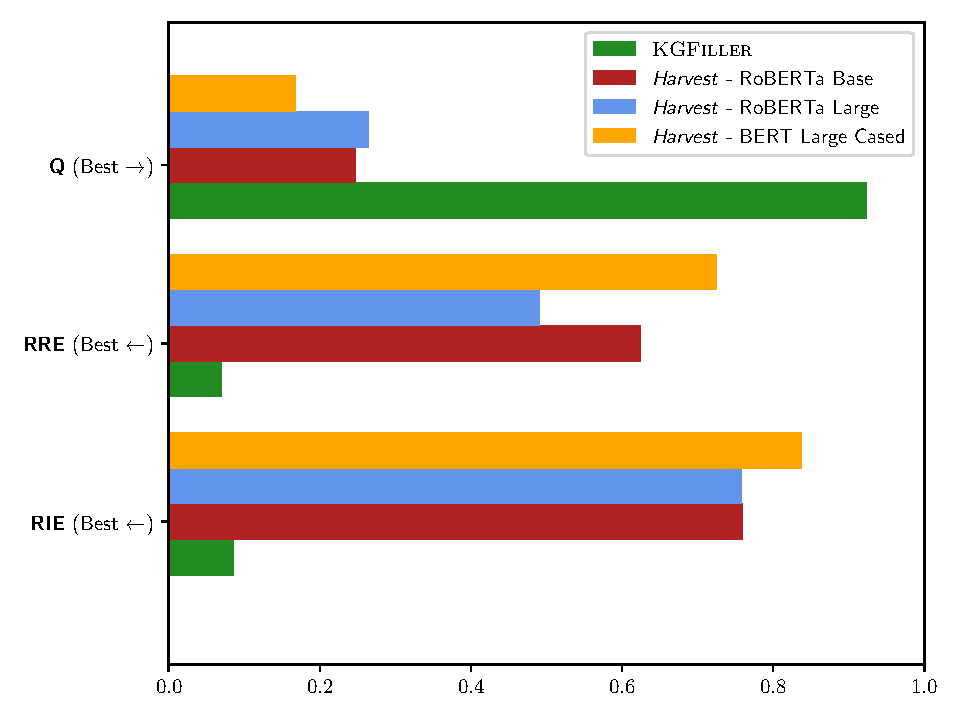
\includegraphics[width=\linewidth]{figures/kgfiller/comparison}
    \caption[Performance Comparison of Harvest and \llmfkg{}]{
        Performance comparison of Harvest~\cite{HaoTTNSZXH23} and \llmfkg{} for populating the food ontology (\Cref{subsubsec:kgfiller-ontology}).
        %
        The best-performing closed-source and open-source \gls{LLM} models are considered: GPT 3.5 Turbo and Nous Hermes, respectively.
    }
    \label{fig:compare-performance}
\end{figure}



\subsection{Discussion and \gls{SWOT} Analysis}
\label{subsec:discussion}

To the best of our knowledge, this work introduces a novel methodology for ontology population, enabling the generation of structured knowledge tailored to specific domains or schemas.
%
This section provides a \gls{SWOT} analysis, highlighting the \textit{Strengths}, \textit{Weaknesses}, \textit{Opportunities}, and \textit{Threats} of \llmfkg{}.
%
The discussion transitions from technical aspects to strategic considerations, including potential applications, limitations, and future directions.

\subsubsection{Strengths}
\label{subsubsec:strengths}

\paragraph{Automation}
%
\llmfkg{} leverages \glspl{LLM} trained on extensive general-knowledge datasets.
%
This eliminates the need for large \emph{corpora} of textual documents and makes it the first fully automatic ontology population method.
%
No prior domain knowledge representation is required from the user.

\paragraph{Generality}
%
\glspl{LLM} enable \llmfkg{} to operate across virtually any domain, irrespective of the availability of domain-specific data.
%
Unlike traditional methods, which rely on potentially incomplete or biased document collections, \llmfkg{} benefits from the broad and diverse knowledge embedded in \glspl{LLM}.

\paragraph{Incrementality}
%
\llmfkg{} supports both ontology population and refinement.
%
It can be applied iteratively to enrich existing ontologies, allowing for incremental improvements over multiple runs.
%
This flexibility contrasts with traditional methods, which are often constrained by predefined input datasets.

\paragraph{Future Potential}

As \glspl{LLM} continue to evolve, their emergent capabilities are expected to enhance the quality of ontology population.
%
Future advancements may enable \llmfkg{} to extract knowledge beyond the explicit content of training data.

\subsubsection{Weaknesses}
\label{subsubsec:weaknesses}
%
\paragraph{Completeness}
%
\llmfkg{} does not guarantee completeness in the populated ontology.
%
Instances or relations may be missing, as the method is not designed to extract all knowledge from the \gls{LLM}.
%
This limitation is inherent to any (semi-)automatic data-driven approach.

\paragraph{Sampling Bias}
%
The reliance on \glspl{LLM} trained on web data introduces potential sampling biases.
%
Underrepresented topics on the web may result in unbalanced or biased ontologies.
%
Further research is needed to mitigate these biases in \glspl{LLM}.

\paragraph{Correctness}
%
\llmfkg{} cannot ensure the correctness of extracted information.
%
\glspl{LLM} are prone to hallucinations, which may lead to the inclusion of false or misleading data in the ontology~\cite{hallucination-2023}.
%
Careful validation of the populated ontology is necessary to address this limitation.


\subsubsection{Opportunities}
\label{subsubsec:opportunities}
%
\paragraph{Cold Start}
%
\llmfkg{} addresses the cold start problem in knowledge-based systems by providing a quick and cost-effective way to generate domain-specific data.
%
This capability is particularly valuable in early-stage projects where data availability is limited.

\paragraph{Automatic Hierarchy Construction}
%
Extensions of \llmfkg{} could enable the automatic construction of ontology schemas, a task often referred to as \emph{hierarchy construction}~\cite{funk2023ontology}.
%
Such advancements could automate the entire ontology creation process, combining schema construction with population.


\paragraph{Zero-Shot Ontology Creation}
%
Building on the idea of hierarchy construction, \llmfkg{} could be adapted to create ontologies from scratch.
%
This would involve generating both the schema and instances based on a natural-language description of the domain.

\paragraph{Procedural Knowledge Extraction}
%
\llmfkg{} could be extended to extract procedural knowledge, representing structured steps to achieve specific goals.
%
This application has potential in fields like automated planning and \glspl{MAS}, where agents require executable plans to perform tasks.


\subsubsection{Threats}
\label{subsubsec:threats}
%
\paragraph{Dependence on \glspl{LLM}}
%
The effectiveness of \llmfkg{} is tied to the quality and capabilities of the underlying \glspl{LLM}.
%
Limitations in \glspl{LLM}, such as biases or inaccuracies, directly impact the quality of the populated ontology.

\paragraph{Cost and Efficiency}
%
The computational and financial costs of querying \glspl{LLM} may pose challenges, especially for large-scale ontology population tasks.
%
Optimizing the process to balance cost and quality remains an open research question.

\paragraph{Ethical Concerns}
%
The use of \glspl{LLM} trained on web data raises ethical concerns, including data privacy and the propagation of biases.
%
Addressing these issues is critical to ensure responsible deployment of \llmfkg{}.

% The SWOT analysis highlights the potential and limitations of \llmfkg{},
% providing a roadmap for future research and development.


\subsection{Conclusion}
\label{subsec:kgfiller-conclusion}
%
Ontologies provide a structured framework to define concepts, relationships, and properties within a specific domain.
%
This ensures an unambiguous and comprehensible representation of domain-specific knowledge.
%
However, the process of ontology population is often meticulous, time-consuming, and prone to human errors and biases.
%

In this work, we hypothesize that \glspl{LLM}\footnote{Defined in \texttt{my\_acronyms.sty}} embed a significant amount of domain-specific knowledge.
%
This knowledge is acquired during their domain-agnostic training on vast datasets collected from the Web.
%
Based on this hypothesis, we propose \llmfkg{}, a novel approach for automatic ontology population leveraging \glspl{LLM}.
%

The proposed method starts with:
%
\begin{inlinelist}
    \item an initial schema consisting of interrelated classes and properties, and
    %
    \item a set of query templates.
\end{inlinelist}
%
\llmfkg{} queries the \gls{LLM} multiple times to generate instances for classes, relationships, and properties based on its responses.
%
Additional queries are performed to refine the ontology, ensuring balanced class hierarchies and avoiding duplicate entries.
%

The validity of \llmfkg{} is demonstrated through a case study in the food domain.
%
This domain requires the population of an ontology with food ingredients, categorized across multiple classes, and recipes.
%
We evaluate \llmfkg{} using various state-of-the-art \glspl{LLM}, including open-source, closed-source, and \glspl{MoE}.
%
The evaluation employs a range of metrics to assess the quality of the constructed ontology.
%

Our results show that \llmfkg{} reliably populates ontologies across different \glspl{LLM}.
%
For instance, the GPT 3.5 model achieves accuracies of up to \(0.91\) for instances and \(0.93\) for relations.
%
As expected, larger \glspl{LLM} generally perform better.
%
We also observe a correlation between erroneous instances and misplaced relations, highlighting areas for improvement.
%

Finally, we analyze the severity of errors, emphasizing how hallucinations from \glspl{LLM} can negatively impact the ontology population process.
%
Despite these challenges, the results are promising.
%
They demonstrate that the complex task of ontology construction can be partially automated, requiring only minor post-processing efforts.
%



\section{Actively learning \EL terminologies from \glspl{LLM}}\label{sec:actively-learning-ontologies}
%
We now present the paper ``Actively Learning \EL Terminologies from Large Language Models'', accepted at the 28th European Conference on Artificial Intelligence (ECAI 2025)\footnote{\url{https://ecai2025.org/}}.
%
In active learning, a \emph{learner} attempts to learn from a \emph{teacher} by posing questions.
%
The questions made by the learner are called \emph{membership queries} and are answered with `yes' or `no'.
%
This kind of query is often studied as part of a communication protocol that also includes \emph{equivalence queries}.
%
Intuitively, equivalence queries ask whether the idea of the learner about the knowledge of the teacher is correct or not.
%
If not, then the teacher should provide a counterexample showing the difference (or equivalently, with `true' or `false').
%
In this work, we consider the teacher as a \gls{LLM} and study the case in which knowledge is expressed as an \EL terminology.
%
Membership queries ask whether concept inclusions are true or not.
%
Equivalence queries are simulated by a sample with concept inclusions labelled as  positive or negative.
%
We present a non-trivial extension of the ExactLearner tool to extract \EL terminologies from \glspl{LLM}.
%
The ExactLearner was originally designed to run with a synthetic teacher that answers membership queries together with equivalence queries.
%
Given the relevant symbols as input (e.g., algae, plant, etc.), the tool tries to find how these symbols should be logically connected by posing questions to \glspl{LLM}.
%
To evaluate the approach, we present performance results of the ExactLearner in the task of reconstructing existing \EL terminologies.


\subsection{Introduction}
\label{subsec:actively-learning-introduction}
\glspl{LLM} have accumulated vast amounts of information and significantly improved their question-answering capabilities.
%
This has led to the development of methods to interact with and extract knowledge from these models.
%
Prompts to \glspl{LLM} range from general knowledge questions, such as definitions and historical events, to domain-specific queries, such as scientific facts in health and medicine.
%
Recent efforts have focused on automating the extraction of knowledge from \glspl{LLM}, often representing this knowledge in the form of an \emph{ontology}~\cite{10.1093/bioinformatics/btae104,DBLP:journals/kbs/CiattoAMO25,DBLP:conf/ekaw/DurantiGMRR24,DBLP:conf/kbclm/2023,DBLP:conf/ontobras/SoaresW24}.
%
Ontologies, a cornerstone of \gls{KR}, provide a structured representation of the conceptual knowledge within a domain.
%
The most widely used formalism for specifying ontologies is \emph{description logic}~\cite{DBLP:books/daglib/0041477}.
%
In life sciences, ontologies are extensively used for tasks such as data integration, information retrieval, and automated reasoning~\cite{DBLP:conf/semweb/NoySDDGJMRYM08}.

%
A key question arises: \emph{What can we learn from \glspl{LLM}?}
%
Moreover, given that \glspl{LLM} can produce incorrect or inconsistent information, is there an automated way to identify such inaccuracies?
%
To address these questions, this work explores an active learning approach to construct \emph{description logic ontologies} from \glspl{LLM}.
%
Our approach is grounded in Angluin's exact learning framework~\cite{DBLP:journals/ml/Angluin87}, where a \emph{learner} acquires knowledge from a \emph{teacher} by posing queries.
%
This method, known as \emph{active learning}~\cite{DBLP:conf/stoc/Angluin92}, involves two types of queries: \emph{membership queries} and \emph{equivalence queries}.
%
Here, we consider the \gls{LLM} as the teacher and aim to learn ontologies formulated in the \EL description logic~\cite{DBLP:conf/ijcai/BaaderBL05}.

%
Exact learning of lightweight description logic ontologies has been studied extensively for theoretical purposes~\cite{DBLP:conf/ijcai/FunkJLPW19,DBLP:conf/ijcai/FunkJL21,DBLP:conf/aaai/KonevOW16,DBLP:journals/jmlr/KonevLOW17,DBLP:conf/dlog/OzakiPM20}.
%
However, a major challenge in applying these algorithms is finding a suitable teacher capable of answering the required queries.
%
The only known implementation for exact learning of \EL ontologies is the \emph{ExactLearner} tool~\cite{DBLP:conf/kr/DuarteKO18}.
%
This tool learns \EL terminologies\footnote{An \EL terminology is an ontology with specific syntactic restrictions (see Sec.~\ref{sec:active-learning-ontologies}).} from a synthetic teacher that can answer membership and equivalence queries.
%
Membership queries verify whether a given concept inclusion is true or false, while equivalence queries check whether the learner's hypothesis matches the teacher's knowledge.
%
If the hypothesis is incorrect, the teacher provides a counterexample.

%
The synthetic teacher in \emph{ExactLearner} was designed to test the tool using ontologies from the Oxford Ontology Repository\footnote{\url{https://www.cs.ox.ac.uk/isg/ontologies/}}.
%
Given a set of relevant symbols, referred to as the \emph{vocabulary} or \emph{signature} (e.g., algae, plant), the tool determines how these symbols are logically connected by posing queries to the teacher.

%
In this work, we extend the \emph{ExactLearner} tool to interact with \glspl{LLM} as teachers, naming the extended version \emph{ExactLearner+LLM}.
%
We use the Manchester OWL Syntax~\cite{DBLP:conf/owled/HorridgeDGRSW06} and a custom parsing function to translate concept inclusions from description logic into natural language.
%
While membership queries can be directly mapped to a question-answering setting with \glspl{LLM}, equivalence queries are more challenging~\cite{DBLP:journals/ml/WeissGY24,DBLP:journals/ijar/BlumKOT24}.
%
To address this, we simulate equivalence queries using a sample of randomly generated concept inclusions classified as true or false by the \gls{LLM}.
%
This approach aligns with the theoretical analysis of Angluin's framework within the \gls{PAC} learning paradigm~\cite{DBLP:journals/ml/Angluin87}.

%
To evaluate our approach, we conducted experiments using \emph{ExactLearner+LLM} with open-source \glspl{LLM}.
%
The tool was provided with a signature and tasked with reconstructing existing ontologies.
%
We tested it on small ontologies from the original \emph{ExactLearner} benchmark and modules extracted from the GALEN ontology~\cite{Rector2008TheGH}, which contains medical terms.
%
Our results also examine whether there is statistical evidence of correlation between the concept inclusions extracted by \emph{ExactLearner+LLM} and those in the original ontologies created by human engineers.
%
% This highlights the potential of \glspl{LLM} in ontology construction.


\subsection{Background and related work}
\label{subsec:actively-learning-background}
%
In this section, we define the concept of an \EL terminology, elaborate on the exact and \gls{PAC} learning frameworks, and describe the algorithm implemented in the \emph{ExactLearner} tool~\cite{DBLP:conf/kr/DuarteKO18}, which is designed to learn \EL terminologies from a teacher capable of answering membership and equivalence queries.
%
\paragraph{The \EL Description Logic}
Let \(\NC\) and \(\NR\) be countably infinite and disjoint sets of \emph{concept names} and \emph{role names}, respectively.
%
In some cases, we may consider \(\NC\) and \(\NR\) as finite sets, depending on the context.
%
An \EL \emph{concept} is defined as \(C, D := C \sqcap D \mid \exists r.C \mid A \mid \top\), where \(A \in \NC\) and \(r \in \NR\).
%
An \EL \emph{concept inclusion} is an expression of the form \(C \sqsubseteq D\), where \(C\) and \(D\) are \EL concepts.
%
An \EL \emph{equivalence} is expressed as \(C \equiv D\), which is equivalent to \(C \sqsubseteq D\) and \(D \sqsubseteq C\).
%
An \EL \emph{ontology} is a finite set of \EL concept inclusions \(C \sqsubseteq D\).
%
For a given ontology \(\Omc\), we denote the sets of concept names and role names occurring in \(\Omc\) as \(\NC(\Omc)\) and \(\NR(\Omc)\), respectively.
%
These sets are also referred to as the \emph{signature} of \(\Omc\).
%
If, for all concept inclusions \(C \sqsubseteq D\) in \(\Omc\), at least one of \(C\) or \(D\) belongs to \(\NC\), and there is at most one inclusion of the form \(A \sqsubseteq C\) for every \(A \in \NC\), then \(\Omc\) is called a \emph{terminology}\footnote{This definition is slightly more flexible than the standard one in the description logic literature~\cite{DBLP:books/daglib/0041477}.}.
%
The semantics of \EL is defined using interpretations, as described in~\cite{DBLP:books/daglib/0041477}.
%
Given an ontology \(\Omc\) and a concept inclusion \(C \sqsubseteq D\), we say that \(\Omc\) \emph{entails} \(C \sqsubseteq D\), denoted as \(\Omc \models C \sqsubseteq D\), if every interpretation satisfying \(\Omc\) also satisfies \(C \sqsubseteq D\).
%
Two ontologies \(\Omc\) and \(\Hmc\) are \emph{equivalent}, denoted as \(\Omc \equiv \Hmc\), if they are satisfied by the same interpretations.
%
This means that, for all concept inclusions \(C \sqsubseteq D\), \(\Omc \models C \sqsubseteq D \iff \Hmc \models C \sqsubseteq D\).


\paragraph{Exact Learning}
The exact learning framework, introduced by Angluin~\cite{DBLP:journals/ml/Angluin87}, involves a \emph{learner} attempting to acquire a target concept, which in this work is an \EL terminology, from a \emph{teacher}.
%
The communication protocol between the learner and the teacher includes two types of queries:
%
\begin{itemize}
    \item \emph{Membership queries}, where the learner asks whether a specific statement is true or false.
    %
    \item \emph{Equivalence queries}, where the learner proposes a hypothesis and receives either confirmation that the hypothesis matches the target or a counterexample highlighting the difference~\cite{DBLP:journals/ml/Angluin87}.
\end{itemize}
%
In our context, membership queries verify whether an \EL concept inclusion \(C \sqsubseteq D\) is true or false.
%
For example, the learner may ask whether \(\mathsf{Algae} \sqsubseteq \mathsf{Plant}\) holds true.


\paragraph{Simulating Equivalence Queries}
To simulate equivalence queries, we adopt a \emph{sampling} strategy.
%
Instead of directly asking the \gls{LLM} to evaluate the hypothesis and provide a counterexample, we generate a random set of \EL concept inclusions and query the \gls{LLM} to classify them as true or false.
%
We then verify whether the learner's hypothesis is consistent with the \gls{LLM}'s classification.
%
Consistency is achieved if all true concept inclusions are logical consequences of the hypothesis and all false inclusions are not.
%
If the hypothesis is consistent, the learning process terminates.
%
Otherwise, a counterexample is identified, and the process continues as if the \gls{LLM} had returned a counterexample in response to an equivalence query.
%
This approach has been used in prior work to simulate equivalence queries~\cite{DBLP:journals/ml/WeissGY24,DBLP:journals/ijar/BlumKOT24}.
%
Under certain conditions, this strategy provides theoretical guarantees within the \gls{PAC} learning framework~\cite{DBLP:journals/ml/Angluin87,DBLP:journals/cacm/Valiant84}.
%
In \gls{PAC} learning, the required sample size is determined by the hypothesis space \(\mathbf{H}\) (in this case, \EL terminologies of a specific size and structure defined by a given signature) and two parameters, \(\epsilon\) and \(\delta\), representing the error tolerance and confidence level, respectively.
%
According to \gls{PAC} theory~\cite[Cor. 2.3]{DBLP:books/daglib/0033642}, the sample size must be at least \(\mathsf{ln}(|\mathbf{H}|/\delta)/\epsilon\) for finite \(\mathbf{H}\).


\paragraph{The Algorithm for \EL Terminologies}
%
\begin{algorithm}
\caption{The learning algorithm for $\mathcal{EL}$~\cite{DBLP:conf/kr/DuarteKO18}}
\label{alg:learn}
\begin{algorithmic}[1]
\State \textbf{Input:} $\NC(\Omc) \cup \NR(\Omc)$ and access to a teacher that can answer membership and equivalence queries (or just membership queries if equivalence queries are simulated in a PAC setting).
\State \textbf{Output:} An $\mathcal{EL}$ terminology $\Hmc$ such that $\Omc \equiv \Hmc$.
\Statex
\State Initialize $\Hmc \gets \{A \sqsubseteq B \mid \Omc \models A \sqsubseteq B, A,B\in \NC(\Omc)\}$
\While{$\Hmc \not\equiv \Omc$} \label{line:while}
    \State Let $C \sqsubseteq D$ be a positive counterexample for $\Omc$ relative to $\Hmc$
    \State Compute $C' \sqsubseteq D'$ with $C'$ or $D'$ in $\NC(\Omc)$
    \label{line:counterexample}
    \If{$C' \in \NC(\Omc)$}
        \State Compute a right $\Omc$-essential $\alpha$ from
        \[
        C' \sqsubseteq D' \sqcap \bigsqcap_{C' \sqsubseteq F' \in \Hmc} F'
        \]
        \label{line:right-essential}
    \Else
        \State Compute a left $\Omc$-essential $\alpha$ from $C' \sqsubseteq D'$
        \label{line:left-essential}
    \EndIf
    \State Add $\alpha$ to $\Hmc$
    \label{line:add-to-hypothesis}
\EndWhile
\State \Return $\Hmc$
\end{algorithmic}
\end{algorithm}
%
The \emph{ExactLearner} tool~\cite{DBLP:conf/kr/DuarteKO18} is designed to learn \EL terminologies by interacting with a synthetic teacher that answers membership and equivalence queries.
%
The teacher's responses are logically consistent with a target \EL terminology, and the communication is conducted in \gls{OWL} rather than natural language.
%
The main steps of the learning procedure are outlined in \Cref{alg:learn}.
%
The algorithm performs equivalence queries in line~\ref{line:while} and membership queries in lines~\ref{line:counterexample},~\ref{line:right-essential}, and~\ref{line:left-essential}.
%
In line~\ref{line:counterexample}, a counterexample \(C' \sqsubseteq D'\) is extracted from \(C \sqsubseteq D\), ensuring that one of the sides belongs to \(\NC(\Omc)\).
%
This step is guaranteed to find a counterexample because \(\Omc\) is a terminology~\cite{DBLP:conf/kr/DuarteKO18}.
%
The algorithm applies various operations using membership queries, including \emph{concept saturation for \(\Omc\)}, \emph{sibling merging}, \emph{decomposition on the right}, and \emph{decomposition on the left}.
%
Additionally, two heuristics, \emph{desaturation} and \emph{branching}, are employed.
%
These operations aim to maximize the informativeness of concept inclusions while minimizing their size.
%
The resulting concept inclusions, referred to as \(\Omc\)-essential, are added to the hypothesis in line~\ref{line:add-to-hypothesis}.


\subsection{\glspl{LLM} as teachers}
\label{subsec:probing}
%
\glspl{LLM} present significant opportunities for acquiring knowledge in the form of ontologies.
%
However, several challenges must be addressed to effectively employ them as teachers in an active learning framework.
%
The main challenges are as follows:
%
\begin{itemize}
    \item Membership queries in the \emph{ExactLearner} tool are expressed in \gls{OWL}, whereas \glspl{LLM} are designed to process natural language inputs.
    %
    \item Responses from \glspl{LLM} may deviate from the expected format, even when explicitly instructed to answer with `yes' or `no'.
    %
    \item Queries generated by the \emph{ExactLearner} can be lengthy and complex, involving multiple logical operators, which may hinder the ability of \glspl{LLM} to provide accurate answers.
    %
    \item Even when responses are concise and well-formatted, they may be logically inconsistent with previous answers or incorrect, and they may vary if the same query is repeated.
    %
    \item The expressivity of the ontology language used (\EL) limits the scope of the knowledge that can be extracted.
\end{itemize}
%
Below, we discuss how these challenges are addressed.


\paragraph{Input Format}
\label{par:input-format}
%
The format of the queries plays a crucial role in ensuring effective communication with \glspl{LLM}.
%
We use both the Manchester \gls{OWL} syntax~\cite{DBLP:conf/owled/HorridgeDGRSW06} and controlled natural language to standardize the queries.
%
Queries in Manchester \gls{OWL} syntax take the form \texttt{[A] SubClassOf [B]}.
%
In natural language, these are translated into questions such as:
%
\begin{center}
    ``Can \texttt{[A]} be considered a subcategory of \texttt{[B]}? Answer only with yes or no.''
\end{center}
%
Here, \texttt{[A]} and \texttt{[B]} are placeholders for the left-hand and right-hand sides of the concept inclusion.
%
This approach aligns with the third formulation proposed by Funk et al.~\cite{DBLP:conf/kbclm/2023}, which is well-suited to our setting.
%
The translation of \gls{OWL} concept expressions into natural language is applied recursively:
%
\begin{enumerate}
    \item Expressions of the form \texttt{[A] and [B]} are replaced with ``\texttt{[A]} that is also \texttt{[B]}''.
    %
    \item Expressions of the form \texttt{[r] some [A]}, where \texttt{[r]} is a role name, are replaced with ``something that \texttt{[r]} \texttt{[A]}''.
\end{enumerate}
%
\begin{example}\upshape
    The concept inclusion \texttt{Person SubClassOf Human} is translated into:
    %
    ``Can Person be considered a subcategory of Human?''
    %
    Similarly, \texttt{Carnivore SubClassOf Animal and eats some Meat} becomes:
    %
    ``Can Carnivore be considered a subcategory of Animal that is also something that eats Meat?''
    %
    Finally, \texttt{(Bird and Fish) SubClassOf Animal} is translated to:
    %
    ``Can Bird that is also Fish be considered a subcategory of Animal?''
\end{example}


\paragraph{Unexpected Responses}
\label{par:unexpected-responses}
%
\glspl{LLM} may return arbitrary responses, even when the expected answer is a single word such as `true' or `false'.
%
To mitigate this, we explicitly instruct the \gls{LLM} to answer with `true' or `false' by appending this requirement to the query.
%
Alternatively, we use system prompts or adjust hyperparameters, such as temperature, to guide the model's responses.
%
Despite these precautions, unexpected responses may still occur:
%
\begin{enumerate}
    \item The response may include additional text beyond `true' or `false'.
    %
    \item Both `true' and `false' may appear in the response.
    %
    \item Neither `true' nor `false' may be present in the response.
\end{enumerate}
%
To address these issues, we limit the maximum number of tokens in the response.
%
If the response does not contain `true' or `false', we treat it as `false'.


\paragraph{Length of Queries}
\label{par:length-of-queries}
%
Long and complex queries can lead to biased responses from \glspl{LLM}, such as always answering `true'.
%
To address this, we modify the \emph{ExactLearner} tool as follows:
%
\begin{itemize}
    \item \emph{Simplification:} Concept expressions are simplified by removing redundant concept names.
    %
    For example, if $A \sqcap B$ is a concept expression and $A \sqsubseteq B$ is entailed by the hypothesis, $B$ is omitted.
    %
    \item \emph{Splitting:} Long queries with multiple conjuncts are split into smaller queries.
    %
    For instance, instead of asking whether $C \sqsubseteq D_1 \sqcap \ldots \sqcap D_n$, we ask whether $C \sqsubseteq D_1$, $C \sqsubseteq D_2$, and so on.
\end{itemize}
%
These modifications reduce the likelihood of biased responses and improve the accuracy of the \gls{LLM}.


\paragraph{Correctness and Logical Consistency}
\label{par:correctness-and-consistency}
%
Responses from \glspl{LLM} may not always reflect the truth or be logically consistent with an \EL ontology.
%
Errors can occur in the following cases:
%
\begin{enumerate}
    \item A false inclusion $C \sqsubseteq D$ is incorrectly answered as `true'.
    %
    \item A true inclusion $C \sqsubseteq D$ is incorrectly answered as `false'.
    %
    \item The \gls{LLM} answers `true' for all inclusions in an ontology $\Omc$, but answers `false' for a logical consequence of $\Omc$.
\end{enumerate}
%
To handle logical inconsistencies, we compute the \emph{closure} under logical consequence~\cite{BLUM2023109026}.
%
Additionally, we use a caching mechanism to store the first response to each query, ensuring consistency across repeated queries.

%
\paragraph{Expressivity}
\label{par:expressivity}
%
The algorithm focuses on extracting \EL terminologies, which may not fully capture knowledge better expressed in more expressive languages.
%
However, \EL is widely used in real-world ontologies, particularly in the medical domain~\cite{Rector2008TheGH,bioportal}.
%
Its polynomial-time reasoning complexity~\cite{DBLP:conf/ijcai/BaaderBL05} and the availability of efficient reasoning tools~\cite{DBLP:journals/jar/KazakovKS14} make it a practical choice for ontology construction.



\subsection{Experiments}
\label{subsec:experiments}

The code for the experiments is publicly available on GitHub\footnote{\url{https://github.com/MatteoMagnini/ExactLearner-LLM/}}.
%
All experiments were conducted on a workstation equipped with two NVIDIA Tesla V100S-PCIE-32GB GPUs and dual Intel\textcopyright~Xeon\textcopyright~Gold 6226R CPUs, providing a total of 64 threads.
%
The system was configured with CUDA 12.5 and NVIDIA driver version 535.183.01.
%

\paragraph{Evaluation Approach}
\Cref{alg:learn} takes as input the signature, which consists of finite sets of concept and role names, and constructs an \gls{EL} terminology by posing membership and equivalence queries.
%
Equivalence queries are simulated using a \emph{\gls{PAC} sample}, which is a set of concept inclusions randomly generated and answered by the \gls{LLM}.
%
For an ontology \(\Omc\) with \(n\) logical axioms, the \gls{PAC} sample size is computed as:
\[
\frac{\ln(A^n / \delta)}{\epsilon},
\]
where \(\delta = 0.1\), \(\epsilon = 0.2\), and \(A\) is the number of all possible axioms of the form:
\[
A \sqsubseteq B, \quad A \sqcap B \sqsubseteq C, \quad B \sqsubseteq \exists r.A, \quad \text{and} \quad \exists r.A \sqsubseteq B,
\]
with \(A, B, C \in \NC\) and \(r \in \NR\), formulated using the signature of \(\Omc\).
%
We refer to these axioms as \emph{normalized}.
%
The ability of ExactLearner+LLM to reconstruct existing ontologies is tested by posing queries to the \gls{LLM}.
%

\paragraph{Hypotheses}
We test the following hypotheses in our experiments:
%
\begin{enumerate}
    \item Even though \glspl{LLM} may make mistakes and the simulation strategy does not guarantee exact learnability, we expect a correlation between the ontologies built by ExactLearner+LLM and the original ontologies.
    %
    \item Queries expressed in controlled natural language using our parsing function will yield better results than those using the OWL Manchester syntax.
    %
    \item Larger \glspl{LLM} will perform better than smaller ones.
    %
    \item Ontologies expressing common knowledge, such as family relations, will be easier to learn than those with specialized knowledge, such as medical ontologies.
    %
    \item Simplifications introduced to reduce query length (see \Cref{sec:probing}) will improve the performance of \glspl{LLM} and, consequently, the ontologies constructed by ExactLearner+LLM.
\end{enumerate}
%

\paragraph{Datasets}
We use two datasets:
%
\begin{enumerate}
    \item Five small ontologies from the ExactLearner benchmark~\cite{DBLP:conf/kr/DuarteKO18}.
    %
    \item Ten modules extracted from the GALEN ontology~\cite{Rector2008TheGH}, which contains medical information.
\end{enumerate}
%
The small ontologies include:
%
\begin{itemize}
    \item \emph{Animals}, which describes the animal realm, including subphyla, classes, and orders.
    %
    \item \emph{Cell}, which provides information about cells based on type, development stage, and organism.
    %
    \item \emph{Football}, a minimal ontology describing relations between football games, teams, players, and managers.
    %
    \item \emph{Generations}, which describes family members and their relations.
    %
    \item \emph{University}, focusing on the professor role.
\end{itemize}
%
\Cref{tab:small-ontologies} summarizes the size of the signature, logical axioms, \gls{PAC} sample size, and possible normalized axioms for these ontologies.
\begin{table}[]
\centering
\caption[Small Ontologies Statistics and \gls{PAC} Sample Sizes]{
    Ontology statistics and \glsentryshort{PAC} sample sizes with $\epsilon=0.2$ and $\gamma=0.1$.
    $\NC$ and $\NR$ are the number of concept and role names occurring in the ontologies.
}
\label{tab:small-ontologies}
\resizebox{\columnwidth}{!}{
\begin{tabular}{|l|c|c|c|c|c|}
\hline
\textbf{Ontology} & \textbf{$\NC$} & \textbf{$\NR$} & \textbf{Log. Ax.} & \textbf{PAC Sample} & \textbf{Poss. Ax.} \\
\hline
\rowcolor[HTML]{EFEFEF}
Animals & 17 & 4 & 12 & 542 & 6,936\\
\hline
\rowcolor[HTML]{FFFFFF}
Cell & 22 & 0 & 24 & 1,119 & 10,164\\
\hline
\rowcolor[HTML]{EFEFEF}
Football & 10 & 3 & 9 & 341 & 1,500\\
\hline
\rowcolor[HTML]{FFFFFF}
Generations & 20 & 4 & 18 & 847 & 10,800\\
\hline
\rowcolor[HTML]{EFEFEF}
University & 7 & 3 & 4 & 139 & 588\\
\hline
\end{tabular}}
\end{table}

%

The GALEN ontology is a large medical ontology with \(22,286\) concept names, \(950\) role names, and \(46,558\) logical axioms.
%
Since not all axioms are connected, we modularize GALEN using the bottom locality strategy~\cite{DBLP:journals/jair/GrauHKS08}\footnote{\url{https://github.com/ernestojimenezruiz/locality-module-extractor}}.
%
This method generates \(22,286\) modules, one for each concept name.
%
We randomly select 10 modules, ensuring each has at least one concept and one role name, and no more than 50 concept or role names.
%
\Cref{tab:modules-ontologies} lists the selected modules.
\begin{table}[]
\centering
\caption{Ontology statistics and \gls{PAC} sample sizes with $\epsilon=0.2$ and $\gamma=0.1$ for medical ontologies.}
\label{tab:modules-ontologies}
\resizebox{\columnwidth}{!}{
\begin{tabular}{|l|c|c|c|c|c|}
\hline
\textbf{Ontology} & \textbf{\NC} & \textbf{\NR} & \textbf{Log. Ax.} & \textbf{PAC Sample}  & \textbf{Pos. Ax.}  \\
\hline
\rowcolor[HTML]{EFEFEF}
Ab. Elb. J. C. & 27 & 14 & 43 & 2,286 & 39,366\\
\hline
\rowcolor[HTML]{FFFFFF}
BNF Sec. & 36 & 24 & 80 & 4,646 & 107,568\\
\hline
\rowcolor[HTML]{EFEFEF}
Chlorhexidine & 23 & 14 & 38 & 1,946 & 26,450\\
\hline
\rowcolor[HTML]{FFFFFF}
Cone of Tissue & 42 & 42 & 100 & 6,163 & 220,500\\
\hline
\rowcolor[HTML]{EFEFEF}
Kalli Krein & 18 & 10 & 27 & 1,279 & 11,988\\
\hline
\rowcolor[HTML]{FFFFFF}
Neon & 16 & 10 & 25 & 1,149 & 8,960\\ 
\hline
\rowcolor[HTML]{EFEFEF}
Pin & 43 & 40 & 99 & 6,113 & 225,578\\
\hline
\rowcolor[HTML]{FFFFFF}
Pros. Drug & 29 & 14 & 47 & 2,540 & 47,096\\
\hline
\rowcolor[HTML]{EFEFEF}
Zopiclone & 32 & 36 & 77 & 4,465 & 105,472\\
\hline
\rowcolor[HTML]{FFFFFF}
Zuccini & 33 & 22 & 58 & 3,295 & 82,764\\
\hline
\end{tabular}}
\end{table}

%

\paragraph{LLMs, Query Format, and Prompts}
We use four open \glspl{LLM}: Mistral~\cite{mistral} (7B parameters), Mixtral~\cite{mixtral} (47B parameters), Llama2 (13B parameters), and Llama3 (8B parameters)~\cite{llama2}, accessed via Ollama's API\footnote{\url{https://github.com/ollama/ollama}}.
%
Queries are expressed in either Manchester OWL syntax or controlled natural language (see \Cref{par:format}).
%
We use two system prompts:
%
\begin{promptbox}[Simple system prompt]
    \scriptsize
    Answer with only True or False.
\end{promptbox}
%
\begin{promptbox}[Advanced system prompt]
    \scriptsize
    You need to classify the following statements as True or False. The statement will be provided in either Manchester OWL syntax or natural language. Strictly follow these guidelines:

    1. Answer with only True or False.

    2. Entities with \texttt{has part} relations are not in a subclass relation.

    3. Statements containing numerous entities are most probably False.

    4. Take a deep breath before answering.

    5. If unsure, answer False.
\end{promptbox}
%
The advanced prompt provides additional contextual information and guidelines to improve \gls{LLM} performance.
%
For instance, it emphasizes that entities with \texttt{has part} relations should not be in a subclass relation~\cite{DBLP:conf/kbclm/2023}.
%
It also mitigates the tendency of \glspl{LLM} to answer ``True'' to long queries, which may arise during the computation of \(\Omc\)-essential concept inclusions (\Cref{subsec:active-learning-ontologies}).
%

\paragraph{Experimental Details}
To constrain \gls{LLM} responses, we limit the maximum number of tokens to 2, ensuring answers are either ``True'' or ``False''\footnote{A token is a unit of text, typically corresponding to a few characters. For example, ``False'' requires 2 tokens. See \url{https://help.openai.com/en/articles/4936856}.}.
%
We also employ a caching mechanism to store \gls{LLM} responses, reducing computation time and ensuring consistency when the same query is posed multiple times.
%
%! Author = matteomagnini
%! Date = 05/03/25

%----------------------------------------------------------------------------------------
\chapter{Conclusions}
\label{ch:conclusions}
\minitoc
%----------------------------------------------------------------------------------------

\section{Discussion}\label{sec:discussion}

\section{Future work}\label{sec:future-work}
\printbibliography[title=References,heading=bibintoc]
\end{refsection}

\adjustmtc

\end{document}